\documentclass[a4paper]{article}

    \usepackage[breakable]{tcolorbox}
    \usepackage{parskip} % Stop auto-indenting (to mimic markdown behaviour)
    

    % Basic figure setup, for now with no caption control since it's done
    % automatically by Pandoc (which extracts ![](path) syntax from Markdown).
    \usepackage[table]{xcolor}
\usepackage{graphicx}
    % Keep aspect ratio if custom image width or height is specified
    \setkeys{Gin}{keepaspectratio}
    % Maintain compatibility with old templates. Remove in nbconvert 6.0
    \let\Oldincludegraphics\includegraphics
    % Ensure that by default, figures have no caption (until we provide a
    % proper Figure object with a Caption API and a way to capture that
    % in the conversion process - todo).
    \usepackage{caption}
    

    \usepackage{float}
    \floatplacement{figure}{H} % forces figures to be placed at the correct location
    \usepackage{xcolor} % Allow colors to be defined
    \usepackage{enumerate} % Needed for markdown enumerations to work
    \usepackage{geometry} % Used to adjust the document margins
    \usepackage{amsmath} % Equations
    \usepackage{amssymb} % Equations
    \usepackage{textcomp} % defines textquotesingle
    % Hack from http://tex.stackexchange.com/a/47451/13684:
    \AtBeginDocument{%
        \def\PYZsq{\textquotesingle}% Upright quotes in Pygmentized code
    }
    \usepackage{upquote} % Upright quotes for verbatim code
    \usepackage{eurosym} % defines \euro

    \usepackage{iftex}
    \ifPDFTeX
        \usepackage[T1]{fontenc}
        \IfFileExists{alphabeta.sty}{
              \usepackage{alphabeta}
          }{
              \usepackage[mathletters]{ucs}
              \usepackage[utf8x]{inputenc}
          }
    \else
        \usepackage{fontspec}
        \usepackage{unicode-math}
    \fi

    \usepackage{fancyvrb} % verbatim replacement that allows latex
    \usepackage{grffile} % extends the file name processing of package graphics
                         % to support a larger range
    \makeatletter % fix for old versions of grffile with XeLaTeX
    \@ifpackagelater{grffile}{2019/11/01}
    {
      % Do nothing on new versions
    }
    {
      \def\Gread@@xetex#1{%
        \IfFileExists{"\Gin@base".bb}%
        {\Gread@eps{\Gin@base.bb}}%
        {\Gread@@xetex@aux#1}%
      }
    }
    \makeatother
    \usepackage[Export]{adjustbox} % Used to constrain images to a maximum size
    \adjustboxset{max size={0.9\linewidth}{0.9\paperheight}}

    % The hyperref package gives us a pdf with properly built
    % internal navigation ('pdf bookmarks' for the table of contents,
    % internal cross-reference links, web links for URLs, etc.)
    \usepackage{hyperref}
    % The default LaTeX title has an obnoxious amount of whitespace. By default,
    % titling removes some of it. It also provides customization options.
    \usepackage{titling}
    \usepackage{longtable} % longtable support required by pandoc >1.10
    \usepackage{booktabs}  % table support for pandoc > 1.12.2
    \usepackage{array}     % table support for pandoc >= 2.11.3
    \usepackage{calc}      % table minipage width calculation for pandoc >= 2.11.1
    \usepackage[inline]{enumitem} % IRkernel/repr support (it uses the enumerate* environment)
    \usepackage[normalem]{ulem} % ulem is needed to support strikethroughs (\sout)
                                % normalem makes italics be italics, not underlines
    \usepackage{soul}      % strikethrough (\st) support for pandoc >= 3.0.0
    \usepackage{mathrsfs}
    

    
    % Colors for the hyperref package
    \definecolor{urlcolor}{rgb}{0,.145,.698}
    \definecolor{linkcolor}{rgb}{.71,0.21,0.01}
    \definecolor{citecolor}{rgb}{.12,.54,.11}

    % ANSI colors
    \definecolor{ansi-black}{HTML}{3E424D}
    \definecolor{ansi-black-intense}{HTML}{282C36}
    \definecolor{ansi-red}{HTML}{E75C58}
    \definecolor{ansi-red-intense}{HTML}{B22B31}
    \definecolor{ansi-green}{HTML}{00A250}
    \definecolor{ansi-green-intense}{HTML}{007427}
    \definecolor{ansi-yellow}{HTML}{DDB62B}
    \definecolor{ansi-yellow-intense}{HTML}{B27D12}
    \definecolor{ansi-blue}{HTML}{208FFB}
    \definecolor{ansi-blue-intense}{HTML}{0065CA}
    \definecolor{ansi-magenta}{HTML}{D160C4}
    \definecolor{ansi-magenta-intense}{HTML}{A03196}
    \definecolor{ansi-cyan}{HTML}{60C6C8}
    \definecolor{ansi-cyan-intense}{HTML}{258F8F}
    \definecolor{ansi-white}{HTML}{C5C1B4}
    \definecolor{ansi-white-intense}{HTML}{A1A6B2}
    \definecolor{ansi-default-inverse-fg}{HTML}{FFFFFF}
    \definecolor{ansi-default-inverse-bg}{HTML}{000000}

    % common color for the border for error outputs.
    \definecolor{outerrorbackground}{HTML}{FFDFDF}

    % commands and environments needed by pandoc snippets
    % extracted from the output of `pandoc -s`
    \providecommand{\tightlist}{%
      \setlength{\itemsep}{0pt}\setlength{\parskip}{0pt}}
    \DefineVerbatimEnvironment{Highlighting}{Verbatim}{commandchars=\\\{\}}
    % Add ',fontsize=\small' for more characters per line
    \newenvironment{Shaded}{}{}
    \newcommand{\KeywordTok}[1]{\textcolor[rgb]{0.00,0.44,0.13}{\textbf{{#1}}}}
    \newcommand{\DataTypeTok}[1]{\textcolor[rgb]{0.56,0.13,0.00}{{#1}}}
    \newcommand{\DecValTok}[1]{\textcolor[rgb]{0.25,0.63,0.44}{{#1}}}
    \newcommand{\BaseNTok}[1]{\textcolor[rgb]{0.25,0.63,0.44}{{#1}}}
    \newcommand{\FloatTok}[1]{\textcolor[rgb]{0.25,0.63,0.44}{{#1}}}
    \newcommand{\CharTok}[1]{\textcolor[rgb]{0.25,0.44,0.63}{{#1}}}
    \newcommand{\StringTok}[1]{\textcolor[rgb]{0.25,0.44,0.63}{{#1}}}
    \newcommand{\CommentTok}[1]{\textcolor[rgb]{0.38,0.63,0.69}{\textit{{#1}}}}
    \newcommand{\OtherTok}[1]{\textcolor[rgb]{0.00,0.44,0.13}{{#1}}}
    \newcommand{\AlertTok}[1]{\textcolor[rgb]{1.00,0.00,0.00}{\textbf{{#1}}}}
    \newcommand{\FunctionTok}[1]{\textcolor[rgb]{0.02,0.16,0.49}{{#1}}}
    \newcommand{\RegionMarkerTok}[1]{{#1}}
    \newcommand{\ErrorTok}[1]{\textcolor[rgb]{1.00,0.00,0.00}{\textbf{{#1}}}}
    \newcommand{\NormalTok}[1]{{#1}}

    % Additional commands for more recent versions of Pandoc
    \newcommand{\ConstantTok}[1]{\textcolor[rgb]{0.53,0.00,0.00}{{#1}}}
    \newcommand{\SpecialCharTok}[1]{\textcolor[rgb]{0.25,0.44,0.63}{{#1}}}
    \newcommand{\VerbatimStringTok}[1]{\textcolor[rgb]{0.25,0.44,0.63}{{#1}}}
    \newcommand{\SpecialStringTok}[1]{\textcolor[rgb]{0.73,0.40,0.53}{{#1}}}
    \newcommand{\ImportTok}[1]{{#1}}
    \newcommand{\DocumentationTok}[1]{\textcolor[rgb]{0.73,0.13,0.13}{\textit{{#1}}}}
    \newcommand{\AnnotationTok}[1]{\textcolor[rgb]{0.38,0.63,0.69}{\textbf{\textit{{#1}}}}}
    \newcommand{\CommentVarTok}[1]{\textcolor[rgb]{0.38,0.63,0.69}{\textbf{\textit{{#1}}}}}
    \newcommand{\VariableTok}[1]{\textcolor[rgb]{0.10,0.09,0.49}{{#1}}}
    \newcommand{\ControlFlowTok}[1]{\textcolor[rgb]{0.00,0.44,0.13}{\textbf{{#1}}}}
    \newcommand{\OperatorTok}[1]{\textcolor[rgb]{0.40,0.40,0.40}{{#1}}}
    \newcommand{\BuiltInTok}[1]{{#1}}
    \newcommand{\ExtensionTok}[1]{{#1}}
    \newcommand{\PreprocessorTok}[1]{\textcolor[rgb]{0.74,0.48,0.00}{{#1}}}
    \newcommand{\AttributeTok}[1]{\textcolor[rgb]{0.49,0.56,0.16}{{#1}}}
    \newcommand{\InformationTok}[1]{\textcolor[rgb]{0.38,0.63,0.69}{\textbf{\textit{{#1}}}}}
    \newcommand{\WarningTok}[1]{\textcolor[rgb]{0.38,0.63,0.69}{\textbf{\textit{{#1}}}}}


    % Define a nice break command that doesn't care if a line doesn't already
    % exist.
    \def\br{\hspace*{\fill} \\* }
    % Math Jax compatibility definitions
    \def\gt{>}
    \def\lt{<}
    \let\Oldtex\TeX
    \let\Oldlatex\LaTeX
    \renewcommand{\TeX}{\textrm{\Oldtex}}
    \renewcommand{\LaTeX}{\textrm{\Oldlatex}}
    % Document parameters
    % Document title
    \title{BTW 2025 Data Science Challenge}
    
    
    
    
    
    
    
% Pygments definitions
\makeatletter
\def\PY@reset{\let\PY@it=\relax \let\PY@bf=\relax%
    \let\PY@ul=\relax \let\PY@tc=\relax%
    \let\PY@bc=\relax \let\PY@ff=\relax}
\def\PY@tok#1{\csname PY@tok@#1\endcsname}
\def\PY@toks#1+{\ifx\relax#1\empty\else%
    \PY@tok{#1}\expandafter\PY@toks\fi}
\def\PY@do#1{\PY@bc{\PY@tc{\PY@ul{%
    \PY@it{\PY@bf{\PY@ff{#1}}}}}}}
\def\PY#1#2{\PY@reset\PY@toks#1+\relax+\PY@do{#2}}

\@namedef{PY@tok@w}{\def\PY@tc##1{\textcolor[rgb]{0.73,0.73,0.73}{##1}}}
\@namedef{PY@tok@c}{\let\PY@it=\textit\def\PY@tc##1{\textcolor[rgb]{0.24,0.48,0.48}{##1}}}
\@namedef{PY@tok@cp}{\def\PY@tc##1{\textcolor[rgb]{0.61,0.40,0.00}{##1}}}
\@namedef{PY@tok@k}{\let\PY@bf=\textbf\def\PY@tc##1{\textcolor[rgb]{0.00,0.50,0.00}{##1}}}
\@namedef{PY@tok@kp}{\def\PY@tc##1{\textcolor[rgb]{0.00,0.50,0.00}{##1}}}
\@namedef{PY@tok@kt}{\def\PY@tc##1{\textcolor[rgb]{0.69,0.00,0.25}{##1}}}
\@namedef{PY@tok@o}{\def\PY@tc##1{\textcolor[rgb]{0.40,0.40,0.40}{##1}}}
\@namedef{PY@tok@ow}{\let\PY@bf=\textbf\def\PY@tc##1{\textcolor[rgb]{0.67,0.13,1.00}{##1}}}
\@namedef{PY@tok@nb}{\def\PY@tc##1{\textcolor[rgb]{0.00,0.50,0.00}{##1}}}
\@namedef{PY@tok@nf}{\def\PY@tc##1{\textcolor[rgb]{0.00,0.00,1.00}{##1}}}
\@namedef{PY@tok@nc}{\let\PY@bf=\textbf\def\PY@tc##1{\textcolor[rgb]{0.00,0.00,1.00}{##1}}}
\@namedef{PY@tok@nn}{\let\PY@bf=\textbf\def\PY@tc##1{\textcolor[rgb]{0.00,0.00,1.00}{##1}}}
\@namedef{PY@tok@ne}{\let\PY@bf=\textbf\def\PY@tc##1{\textcolor[rgb]{0.80,0.25,0.22}{##1}}}
\@namedef{PY@tok@nv}{\def\PY@tc##1{\textcolor[rgb]{0.10,0.09,0.49}{##1}}}
\@namedef{PY@tok@no}{\def\PY@tc##1{\textcolor[rgb]{0.53,0.00,0.00}{##1}}}
\@namedef{PY@tok@nl}{\def\PY@tc##1{\textcolor[rgb]{0.46,0.46,0.00}{##1}}}
\@namedef{PY@tok@ni}{\let\PY@bf=\textbf\def\PY@tc##1{\textcolor[rgb]{0.44,0.44,0.44}{##1}}}
\@namedef{PY@tok@na}{\def\PY@tc##1{\textcolor[rgb]{0.41,0.47,0.13}{##1}}}
\@namedef{PY@tok@nt}{\let\PY@bf=\textbf\def\PY@tc##1{\textcolor[rgb]{0.00,0.50,0.00}{##1}}}
\@namedef{PY@tok@nd}{\def\PY@tc##1{\textcolor[rgb]{0.67,0.13,1.00}{##1}}}
\@namedef{PY@tok@s}{\def\PY@tc##1{\textcolor[rgb]{0.73,0.13,0.13}{##1}}}
\@namedef{PY@tok@sd}{\let\PY@it=\textit\def\PY@tc##1{\textcolor[rgb]{0.73,0.13,0.13}{##1}}}
\@namedef{PY@tok@si}{\let\PY@bf=\textbf\def\PY@tc##1{\textcolor[rgb]{0.64,0.35,0.47}{##1}}}
\@namedef{PY@tok@se}{\let\PY@bf=\textbf\def\PY@tc##1{\textcolor[rgb]{0.67,0.36,0.12}{##1}}}
\@namedef{PY@tok@sr}{\def\PY@tc##1{\textcolor[rgb]{0.64,0.35,0.47}{##1}}}
\@namedef{PY@tok@ss}{\def\PY@tc##1{\textcolor[rgb]{0.10,0.09,0.49}{##1}}}
\@namedef{PY@tok@sx}{\def\PY@tc##1{\textcolor[rgb]{0.00,0.50,0.00}{##1}}}
\@namedef{PY@tok@m}{\def\PY@tc##1{\textcolor[rgb]{0.40,0.40,0.40}{##1}}}
\@namedef{PY@tok@gh}{\let\PY@bf=\textbf\def\PY@tc##1{\textcolor[rgb]{0.00,0.00,0.50}{##1}}}
\@namedef{PY@tok@gu}{\let\PY@bf=\textbf\def\PY@tc##1{\textcolor[rgb]{0.50,0.00,0.50}{##1}}}
\@namedef{PY@tok@gd}{\def\PY@tc##1{\textcolor[rgb]{0.63,0.00,0.00}{##1}}}
\@namedef{PY@tok@gi}{\def\PY@tc##1{\textcolor[rgb]{0.00,0.52,0.00}{##1}}}
\@namedef{PY@tok@gr}{\def\PY@tc##1{\textcolor[rgb]{0.89,0.00,0.00}{##1}}}
\@namedef{PY@tok@ge}{\let\PY@it=\textit}
\@namedef{PY@tok@gs}{\let\PY@bf=\textbf}
\@namedef{PY@tok@ges}{\let\PY@bf=\textbf\let\PY@it=\textit}
\@namedef{PY@tok@gp}{\let\PY@bf=\textbf\def\PY@tc##1{\textcolor[rgb]{0.00,0.00,0.50}{##1}}}
\@namedef{PY@tok@go}{\def\PY@tc##1{\textcolor[rgb]{0.44,0.44,0.44}{##1}}}
\@namedef{PY@tok@gt}{\def\PY@tc##1{\textcolor[rgb]{0.00,0.27,0.87}{##1}}}
\@namedef{PY@tok@err}{\def\PY@bc##1{{\setlength{\fboxsep}{\string -\fboxrule}\fcolorbox[rgb]{1.00,0.00,0.00}{1,1,1}{\strut ##1}}}}
\@namedef{PY@tok@kc}{\let\PY@bf=\textbf\def\PY@tc##1{\textcolor[rgb]{0.00,0.50,0.00}{##1}}}
\@namedef{PY@tok@kd}{\let\PY@bf=\textbf\def\PY@tc##1{\textcolor[rgb]{0.00,0.50,0.00}{##1}}}
\@namedef{PY@tok@kn}{\let\PY@bf=\textbf\def\PY@tc##1{\textcolor[rgb]{0.00,0.50,0.00}{##1}}}
\@namedef{PY@tok@kr}{\let\PY@bf=\textbf\def\PY@tc##1{\textcolor[rgb]{0.00,0.50,0.00}{##1}}}
\@namedef{PY@tok@bp}{\def\PY@tc##1{\textcolor[rgb]{0.00,0.50,0.00}{##1}}}
\@namedef{PY@tok@fm}{\def\PY@tc##1{\textcolor[rgb]{0.00,0.00,1.00}{##1}}}
\@namedef{PY@tok@vc}{\def\PY@tc##1{\textcolor[rgb]{0.10,0.09,0.49}{##1}}}
\@namedef{PY@tok@vg}{\def\PY@tc##1{\textcolor[rgb]{0.10,0.09,0.49}{##1}}}
\@namedef{PY@tok@vi}{\def\PY@tc##1{\textcolor[rgb]{0.10,0.09,0.49}{##1}}}
\@namedef{PY@tok@vm}{\def\PY@tc##1{\textcolor[rgb]{0.10,0.09,0.49}{##1}}}
\@namedef{PY@tok@sa}{\def\PY@tc##1{\textcolor[rgb]{0.73,0.13,0.13}{##1}}}
\@namedef{PY@tok@sb}{\def\PY@tc##1{\textcolor[rgb]{0.73,0.13,0.13}{##1}}}
\@namedef{PY@tok@sc}{\def\PY@tc##1{\textcolor[rgb]{0.73,0.13,0.13}{##1}}}
\@namedef{PY@tok@dl}{\def\PY@tc##1{\textcolor[rgb]{0.73,0.13,0.13}{##1}}}
\@namedef{PY@tok@s2}{\def\PY@tc##1{\textcolor[rgb]{0.73,0.13,0.13}{##1}}}
\@namedef{PY@tok@sh}{\def\PY@tc##1{\textcolor[rgb]{0.73,0.13,0.13}{##1}}}
\@namedef{PY@tok@s1}{\def\PY@tc##1{\textcolor[rgb]{0.73,0.13,0.13}{##1}}}
\@namedef{PY@tok@mb}{\def\PY@tc##1{\textcolor[rgb]{0.40,0.40,0.40}{##1}}}
\@namedef{PY@tok@mf}{\def\PY@tc##1{\textcolor[rgb]{0.40,0.40,0.40}{##1}}}
\@namedef{PY@tok@mh}{\def\PY@tc##1{\textcolor[rgb]{0.40,0.40,0.40}{##1}}}
\@namedef{PY@tok@mi}{\def\PY@tc##1{\textcolor[rgb]{0.40,0.40,0.40}{##1}}}
\@namedef{PY@tok@il}{\def\PY@tc##1{\textcolor[rgb]{0.40,0.40,0.40}{##1}}}
\@namedef{PY@tok@mo}{\def\PY@tc##1{\textcolor[rgb]{0.40,0.40,0.40}{##1}}}
\@namedef{PY@tok@ch}{\let\PY@it=\textit\def\PY@tc##1{\textcolor[rgb]{0.24,0.48,0.48}{##1}}}
\@namedef{PY@tok@cm}{\let\PY@it=\textit\def\PY@tc##1{\textcolor[rgb]{0.24,0.48,0.48}{##1}}}
\@namedef{PY@tok@cpf}{\let\PY@it=\textit\def\PY@tc##1{\textcolor[rgb]{0.24,0.48,0.48}{##1}}}
\@namedef{PY@tok@c1}{\let\PY@it=\textit\def\PY@tc##1{\textcolor[rgb]{0.24,0.48,0.48}{##1}}}
\@namedef{PY@tok@cs}{\let\PY@it=\textit\def\PY@tc##1{\textcolor[rgb]{0.24,0.48,0.48}{##1}}}

\def\PYZbs{\char`\\}
\def\PYZus{\char`\_}
\def\PYZob{\char`\{}
\def\PYZcb{\char`\}}
\def\PYZca{\char`\^}
\def\PYZam{\char`\&}
\def\PYZlt{\char`\<}
\def\PYZgt{\char`\>}
\def\PYZsh{\char`\#}
\def\PYZpc{\char`\%}
\def\PYZdl{\char`\$}
\def\PYZhy{\char`\-}
\def\PYZsq{\char`\'}
\def\PYZdq{\char`\"}
\def\PYZti{\char`\~}
% for compatibility with earlier versions
\def\PYZat{@}
\def\PYZlb{[}
\def\PYZrb{]}
\makeatother


    % For linebreaks inside Verbatim environment from package fancyvrb.
    \makeatletter
        \newbox\Wrappedcontinuationbox
        \newbox\Wrappedvisiblespacebox
        \newcommand*\Wrappedvisiblespace {\textcolor{red}{\textvisiblespace}}
        \newcommand*\Wrappedcontinuationsymbol {\textcolor{red}{\llap{\tiny$\m@th\hookrightarrow$}}}
        \newcommand*\Wrappedcontinuationindent {3ex }
        \newcommand*\Wrappedafterbreak {\kern\Wrappedcontinuationindent\copy\Wrappedcontinuationbox}
        % Take advantage of the already applied Pygments mark-up to insert
        % potential linebreaks for TeX processing.
        %        {, <, #, %, $, ' and ": go to next line.
        %        _, }, ^, &, >, - and ~: stay at end of broken line.
        % Use of \textquotesingle for straight quote.
        \newcommand*\Wrappedbreaksatspecials {%
            \def\PYGZus{\discretionary{\char`\_}{\Wrappedafterbreak}{\char`\_}}%
            \def\PYGZob{\discretionary{}{\Wrappedafterbreak\char`\{}{\char`\{}}%
            \def\PYGZcb{\discretionary{\char`\}}{\Wrappedafterbreak}{\char`\}}}%
            \def\PYGZca{\discretionary{\char`\^}{\Wrappedafterbreak}{\char`\^}}%
            \def\PYGZam{\discretionary{\char`\&}{\Wrappedafterbreak}{\char`\&}}%
            \def\PYGZlt{\discretionary{}{\Wrappedafterbreak\char`\<}{\char`\<}}%
            \def\PYGZgt{\discretionary{\char`\>}{\Wrappedafterbreak}{\char`\>}}%
            \def\PYGZsh{\discretionary{}{\Wrappedafterbreak\char`\#}{\char`\#}}%
            \def\PYGZpc{\discretionary{}{\Wrappedafterbreak\char`\%}{\char`\%}}%
            \def\PYGZdl{\discretionary{}{\Wrappedafterbreak\char`\$}{\char`\$}}%
            \def\PYGZhy{\discretionary{\char`\-}{\Wrappedafterbreak}{\char`\-}}%
            \def\PYGZsq{\discretionary{}{\Wrappedafterbreak\textquotesingle}{\textquotesingle}}%
            \def\PYGZdq{\discretionary{}{\Wrappedafterbreak\char`\"}{\char`\"}}%
            \def\PYGZti{\discretionary{\char`\~}{\Wrappedafterbreak}{\char`\~}}%
        }
        % Some characters . , ; ? ! / are not pygmentized.
        % This macro makes them "active" and they will insert potential linebreaks
        \newcommand*\Wrappedbreaksatpunct {%
            \lccode`\~`\.\lowercase{\def~}{\discretionary{\hbox{\char`\.}}{\Wrappedafterbreak}{\hbox{\char`\.}}}%
            \lccode`\~`\,\lowercase{\def~}{\discretionary{\hbox{\char`\,}}{\Wrappedafterbreak}{\hbox{\char`\,}}}%
            \lccode`\~`\;\lowercase{\def~}{\discretionary{\hbox{\char`\;}}{\Wrappedafterbreak}{\hbox{\char`\;}}}%
            \lccode`\~`\:\lowercase{\def~}{\discretionary{\hbox{\char`\:}}{\Wrappedafterbreak}{\hbox{\char`\:}}}%
            \lccode`\~`\?\lowercase{\def~}{\discretionary{\hbox{\char`\?}}{\Wrappedafterbreak}{\hbox{\char`\?}}}%
            \lccode`\~`\!\lowercase{\def~}{\discretionary{\hbox{\char`\!}}{\Wrappedafterbreak}{\hbox{\char`\!}}}%
            \lccode`\~`\/\lowercase{\def~}{\discretionary{\hbox{\char`\/}}{\Wrappedafterbreak}{\hbox{\char`\/}}}%
            \catcode`\.\active
            \catcode`\,\active
            \catcode`\;\active
            \catcode`\:\active
            \catcode`\?\active
            \catcode`\!\active
            \catcode`\/\active
            \lccode`\~`\~
        }
    \makeatother

    \let\OriginalVerbatim=\Verbatim
    \makeatletter
    \renewcommand{\Verbatim}[1][1]{%
        %\parskip\z@skip
        \sbox\Wrappedcontinuationbox {\Wrappedcontinuationsymbol}%
        \sbox\Wrappedvisiblespacebox {\FV@SetupFont\Wrappedvisiblespace}%
        \def\FancyVerbFormatLine ##1{\hsize\linewidth
            \vtop{\raggedright\hyphenpenalty\z@\exhyphenpenalty\z@
                \doublehyphendemerits\z@\finalhyphendemerits\z@
                \strut ##1\strut}%
        }%
        % If the linebreak is at a space, the latter will be displayed as visible
        % space at end of first line, and a continuation symbol starts next line.
        % Stretch/shrink are however usually zero for typewriter font.
        \def\FV@Space {%
            \nobreak\hskip\z@ plus\fontdimen3\font minus\fontdimen4\font
            \discretionary{\copy\Wrappedvisiblespacebox}{\Wrappedafterbreak}
            {\kern\fontdimen2\font}%
        }%

        % Allow breaks at special characters using \PYG... macros.
        \Wrappedbreaksatspecials
        % Breaks at punctuation characters . , ; ? ! and / need catcode=\active
        \OriginalVerbatim[#1,codes*=\Wrappedbreaksatpunct]%
    }
    \makeatother

    % Exact colors from NB
    \definecolor{incolor}{HTML}{303F9F}
    \definecolor{outcolor}{HTML}{D84315}
    \definecolor{cellborder}{HTML}{CFCFCF}
    \definecolor{cellbackground}{HTML}{F7F7F7}

    % prompt
    \makeatletter
    \newcommand{\boxspacing}{\kern\kvtcb@left@rule\kern\kvtcb@boxsep}
    \makeatother
    \newcommand{\prompt}[4]{
        {\ttfamily\llap{{\color{#2}[#3]:\hspace{3pt}#4}}\vspace{-\baselineskip}}
    }
    

    
    % Prevent overflowing lines due to hard-to-break entities
    \sloppy
    % Setup hyperref package
    \hypersetup{
      breaklinks=true,  % so long urls are correctly broken across lines
      colorlinks=true,
      urlcolor=urlcolor,
      linkcolor=linkcolor,
      citecolor=citecolor,
      }
    % Slightly bigger margins than the latex defaults
    
    \geometry{verbose,tmargin=1in,bmargin=1in,lmargin=1in,rmargin=1in}
    
    

\author{\\Hannes Bachmann\\Emmanuel Diehl\\Georg Gonsior\\Daniel Ricardo Gonzalez Villamizar\\Julius Hanusch\\Clara Hüfner\\Malte Maier-Knop\\Jordan Wenzel Richter\\Ansgar Seidemann\\Moritz Tschöpe\\Felix Wahler\\\\\\\textit{Supervision by}\\Jimmy Pöhlmann\\Claudio Hartmann\\Wolfgang Lehner\\\\\\}
\begin{document}
    
    \maketitle
    
    

    
    

    \thispagestyle{empty}
\newpage\begin{abstract}
\label{abstract}

Accurately forecasting market dynamics, particularly within the
electricity market, is essential for maintaining grid stability and
preventing power outages. This report presents the methodology employed
by the Dresden Database Research Group to forecast day-ahead electricity
prices, which determine the energy prices for the next day upon which
the companies can plan their production, as part of the BTW 2025 Data
Science Challenge. Data from several sources, including weather and
market data, was collected. We used Explainable AI methods to analyze
the data and identify the most important predictors for day-ahead energy
prices. This allowed us to gain deeper insights into the factors
influencing electricity price predictions. Afterward, we compared
several state-of-the-art time series forecasting methods on an extensive
test set to identify the best among them. For this, we considered
Chronos, Temporal Fusion Transformer, and AutoGluon, which are methods
that were shown to perform very well on different kinds of time series
datasets. The models were analyzed, and various approaches were explored
to further enhance their performance, including fine-tuning, ensembling,
architectural adjustments, and additional feature forecasting. After
conducting a six-month benchmark comparing the final models, we
concluded that a fine-tuned large Chronos model performed the best among
all tested. With this approach, we outperformed the baseline on root
mean squared error by a factor of 1.45 and a factor about 1.67 on mean
absolute error.

    \end{abstract}
\thispagestyle{empty}
\newpage
\thispagestyle{empty}
\hypersetup{linkcolor=black}
\tableofcontents
\thispagestyle{empty}
\newpage\section{Introduction}\label{introduction}

    Forecasting market dynamics, including supply, demand, and pricing, is
critical for entities operating within a market environment. Buyers aim
to identify favorable moments for purchasing goods at lower prices,
while sellers seek to optimize production volumes based on demand and
profitability considerations. This is especially relevant in the context
of the electricity market, where the stability of the grid depends on
maintaining a delicate balance between supply and demand. Disruptions to
this equilibrium can significantly affect grid reliability and may lead
to power outages, as noted by Horáček (2010). Consequently, the field of
electricity price forecasting stands as a subject of considerable
relevance for both market participants and academic researchers.
Historically, these predictions have relied on statistical methods such
as ARIMA, SARIMA, and GARCH models with moving averages to predict next
day's prices, as seen in Contreras et al.~(2003) or Nunes et al.~(2008).
In recent years, deep learning has become a prominent feature of these
attempts, with research surpassing the accuracy of those statistic
approaches using deep learning, for example Lago et al.~(2018).
Explainable AI (xAI) approaches have also enabled a greater
understanding of the electricity market, with research such as Tschora
et al.~(2022) being able to identify the importance and weight of
individual influences on the prediction of electricity prices.

This report outlines the methodology employed by the Dresden Database
Research Group to forecast day-ahead electricity prices as part of the
BTW 2025 Data Science Challenge, with a focus on comparing and enhancing
several established time series forecasting methods. Initially, general
domain knowledge related to energy markets and pricing was researched
and presented (see section \ref{gathering-domain-knowledge}~\nameref{gathering-domain-knowledge}). Following
this, multiple data sources influencing day-ahead prices were
identified, including finance, meteorology, and societal data. Various
preprocessing techniques are also discussed. The data underwent thorough
analysis using methods such as explainable machine learning models,
including Temporal Fusion Transformers. Based on this analysis, data
preparation was carried out iteratively. Additionally, the aspect of
feature importance was compared across models (see section \ref{data-sources}~\nameref{data-sources}). In the subsequent section, the models utilized are described
in detail, and intermediate results are presented (see section \ref{visualization-and-story-telling}~\nameref{visualization-and-story-telling}). The models are then compared in a final
benchmark to identify the most optimal model from the available methods
(see section \ref{predictive-modeling}~\nameref{predictive-modeling}). Finally, the report summarizes the
results, reflects on the experience gained, and outlines potential
features for future work (see section \ref{summary-future-work}~\nameref{summary-future-work}).

    \section{Utils}\label{utils}\textit{code omitted - see notebook for the following contents:}\begin{itemize}\tightlist
\item installs and imports
\item base model structure
\item models implementation
\item benchmarking class
\item downloading data
\item loading data
\end{itemize}\section{Gathering Domain
Knowledge}\label{gathering-domain-knowledge}

    Due to the complexity of the German electricity market and the vastness
of factors pertaining to the formation of electricity prices, we began
our efforts with a collection of relevant domain knowledge. The present
section presents our findings on the German energy market, specifically
the day-ahead price and key influences pertaining to its formation. This
exploration then informs both implementation details and data selection
that will be discussed in later sections.

\subsection{The German Energy Market}\label{the-german-energy-market}

\paragraph{Electricity Markets Within
Germany}\label{electricity-markets-within-germany}

As explained by Schumacher et al.~(2015), in electricity markets such as
Germany, the price of electricity is primarily determined by the
instantaneous relationship between energy consumption and energy
production. Energy that has been produced is rarely stored in a quantity
that is meaningful in relation to the prevailing market price. The
market value may therefore fluctuate on a moment-by-moment basis in
response to outages, consumption spikes, or production surges. This
naturally introduces an element of unpredictability, which may not be
conducive to the stability and predictability that procucers and
consumers of electricity require in order to plan and optimize their
operating shedules and procedures. Consequently, submarkets have emerged
that offer longer-term contracts, enabling customers to procure
electricity in advance for a period of up to six years, typically at a
premium for these assurances. Submarkets offering electricity for
shorter periods may also be established, with auctions taking place for
the following day or even intra-day trading. Similar to other markets,
the ability to effectively predict electricity prices is of significant
importance to market players trying to sell or purchase power at both
opportune points in time and price points. It is important to note that
in Germany only approximately 20\% of electricity volume trading occurs
on exchange markets, with the remainder being directly traded between
producers and consumers, usually in an industrial context. Nevertheless,
even contracts that are negotiated directly between consumers and
producers of electricity directly, frequently establish their prices in
accordance with the prices set by the exchanges.

\paragraph{Day-Ahead Prices}\label{day-ahead-prices}

One of the main subarkets established to reduce uncertainty for
consumers and producers of power is the so caled day-ahead-price. As the
main forecast target of the present work, the following subsection
outlines the creation of the day-ahead price, as described in Nestle et
al.~(2009) and Schumacher et al.~(2015). By midday, market participants
submit their bids and offers, which include the quantity and delivery
time for the following day. Based on these aforementioned bids and
offers, a wholesale price for each hour of the forthcoming day is
calculated. Ultimately, the price of electricity is determined by
ranking the offers in descending order of price, with lower-priced
generation given precedence until no more bids and offers can be
matched. The highest production price that is still accepted becomes the
agreed-upon price, resulting in varying margins between producers. For
many goods, their price is mostly driven by profits, initial- and
marginal costs. In the context of the present work, initial costs are
those associated with the installation of power plants and
infrastructure, marginal costs those pertaining to production and
upkeep. Lower-priced electricity generation tends to be that, with low
associated costs. While renewable energy sources may require some
installation costs, they do not have to include fuel prices in their
calculations and can operate with low marginal costs, given good
conditions such as wind or sunshine. Therefore, these conditions affect
the production volume of such lower priced energy and thereby heavily
influences market prices. Examples of this would be either days with low
wind speeds and little sunshine, on which the volume of cheap, renewable
energy would be much lower, raising the need for alternative power
plants to fill the gap with higher priced energy.

\paragraph{Importance of Prediction}\label{importance-of-prediction}

While these dynamic factors are important for providers and customers
for economic planning as previously described, prediction and planning
are also crucial for the grids stability and ability to reliably provide
electricity to consumers. Producers and consumers are grouped in
balancing groups (Bilanzkreis) as described by Dumancic (2024), with
transmission system operators balancing supply and demand.

Should the delicate balance of production and consumption be tilted,
drastic consequences, such as blackouts and outages for electricity
grids could occur as outlined by Horáček (2010). Unplanned imbalance in
the form of over or underproduction of electricity in such a balancing
group is therefore financially penalized, creating further incentives to
make accurate predictions.

\subsection{Conclusion}\label{conclusion}

In this chapter, we give an overview on the complex workings of the
German energy market. We explain the bidding process where producers and
consumer register their offers and demands respectively and the
resulting day-ahead prices are calculated. Furthermore, we discuss the
influence of different energy sources on the resulting prices. Building
on this knowledge, the next chapter gives a detailed overview on the
individual data sources we examined regarding their influence on the
energy prices.

    \section{Data Sources}\label{data-sources}

In order to predict the day-ahead-price as accurately as possible, a
variety of input data was chosen. The following aims to explain and
inform these choices. As seen in Niedermayer (2023) and Hein et
al.~(2020), the installed net rated capacity of electricity in Germany
is steadily increasing. This phenomenon must be taken into account when
analyzing any variable in isolation and observing a raise. According to
Bosch et al.~(2023) and Hein et al.~(2020), main energy sources include
fossil gas, lignite, coal, wind, and photovoltaics. From the production
side, main drivers of energy prices are therefore factors pertaining to
these elements, such as fuel prices or weather conditions. This chapter
explains the different types of data used to represent these sources in
the forecasts. On the consumer side, the selection of pertinent data
poses a more substantial challenge, as their behavior may be more
challenging to categorize than that of, say, the primary five types of
producers. In the context of this study, it was hypothesized that the
majority of energy consumption exhibits periodic patterns that are
evident in the available data, such as time of day and date.
Additionally, data concerning social events was incorporated into the
analysis. Furthermore, data pertaining to electricity production was
also included in the study, as it is conceivable that such data could
influence energy consumption. For instance, meteorological data, such as
temperature, could potentially impact the necessity for heating,
consequently affecting electricity consumption. Finally, the process of
downloading the data in the previous utils section is described and
results of the data analysis are provided.

    \subsection{Data Presentation and
Discussion}\label{data-presentation-and-discussion}

In this section the different data sources and their according data
frame columns are shown and explained. Furthermore, background
information regarding obtaining the data is given, along with the
introduction of issues that will make preprocessing necessary.

    \paragraph{SMARD Electricity Market
Data}\label{smard-electricity-market-data}

SMARD is an information platform for the German electricity market run
by the federal power network agency ``Bundesnetzagentur''. On the SMARD
website there are datasets containing electricity generation, balancing,
consumption and commercial exchanges available for download, and real
time data is updated with high frequency. Furthermore, background
information about these datasets and the electricity is given,
explaining the types and context of available data. This is especially
important for datasets which went through different circumstances or
determination methods within our selected period of time, as these
changes might make some additional preprocessing necessary (as explained
in \ref{smard-data-preprocessing}~\nameref{smard-data-preprocessing}). SMARD presents a reliable
data source due to it being a government backed service, and the wide
variety of datasets downloadable freely.

The dataset contains the columns presented in \nameref{appendix-i-smard-dataset-columns}. Additional
information can be found in the \hyperref[bibliography]{[SMARD user guide, 2024]}.

    \begin{tcolorbox}[breakable, size=fbox, boxrule=1pt, pad at break*=1mm,colback=cellbackground, colframe=cellborder]
\prompt{In}{incolor}{2}{\boxspacing}
\begin{small}
\begin{Verbatim}[commandchars=\\\{\}]
\PY{n}{pd}\PY{o}{.}\PY{n}{read\PYZus{}csv}\PY{p}{(}\PY{l+s+s1}{\PYZsq{}}\PY{l+s+s1}{../final\PYZhy{}submission/merged\PYZus{}data/data\PYZus{}collection/smard.csv}\PY{l+s+s1}{\PYZsq{}}\PY{p}{)}\PY{p}{[}\PY{l+m+mi}{1000}\PY{p}{:}\PY{p}{]}\PY{o}{.}\PY{n}{head}\PY{p}{(}\PY{p}{)}
\end{Verbatim}
\end{small}
\end{tcolorbox}

            \begin{tcolorbox}[breakable, size=fbox, boxrule=.5pt, pad at break*=1mm, opacityfill=0]
\prompt{Out}{outcolor}{2}{\boxspacing}
\begin{small}
\begin{Verbatim}[commandchars=\\\{\}]
                     Date             End\_Date  \textbackslash{}
1000  2015-02-11 16:00:00  2015-02-11 17:00:00
1001  2015-02-11 17:00:00  2015-02-11 18:00:00
1002  2015-02-11 18:00:00  2015-02-11 19:00:00
1003  2015-02-11 19:00:00  2015-02-11 20:00:00
1004  2015-02-11 20:00:00  2015-02-11 21:00:00

      af\_E\_Volume\_Activated\_Plus\_MWh  af\_E\_Volume\_Activated\_Minus\_MWh  \textbackslash{}
1000                             7.0                            239.0
1001                            42.0                            242.0
1002                           276.0                              3.0
1003                           294.0                             59.0
1004                           158.0                             33.0

      af\_Activation\_Price\_Plus\_EUR\_MWh  af\_Activation\_Price\_Minus\_EUR\_MWh  \textbackslash{}
1000                             60.63                             -15.31
1001                             61.36                             -15.55
1002                             64.62                             -16.90
1003                             64.31                             -16.24
1004                             61.25                              -9.18

      af\_E\_Volume\_Procured\_Plus\_MW  af\_E\_Volume\_Procured\_Minus\_MW  \textbackslash{}
1000                        2054.0                         2021.0
1001                        2054.0                         2021.0
1002                        2054.0                         2021.0
1003                        2054.0                         2021.0
1004                        2054.0                         2021.0

      af\_Procurement\_Price\_Plus\_EUR\_MW  af\_Procurement\_Price\_Minus\_EUR\_MW  \textbackslash{}
1000                            385.31                              99.02
1001                            385.31                              99.02
1002                            385.31                              99.02
1003                            385.31                              99.02
1004                            550.54                             247.33

      {\ldots}  E\_AustriaExport\_MWh  E\_AustriaImport\_MWh  E\_FranceExport\_MWh  \textbackslash{}
1000  {\ldots}               5803.0              -1805.0              1514.0
1001  {\ldots}               5741.0              -1822.0              1385.0
1002  {\ldots}               5565.0              -2210.0              2829.0
1003  {\ldots}               5429.0              -2317.0              3000.0
1004  {\ldots}               5245.0              -1698.0              3000.0

      E\_FranceImport\_MWh  E\_PolandExport\_MWh  E\_PolandImport\_MWh  \textbackslash{}
1000                 0.0                 0.0              -433.0
1001              -248.0                 0.0              -258.0
1002              -476.0                 0.0              -398.0
1003                 0.0                 0.0              -393.0
1004               -82.0               150.0              -623.0

      E\_NorwayExport\_MWh  E\_NorwayImport\_MWh  E\_BelgiumExport\_MWh  \textbackslash{}
1000                 NaN                 NaN                  NaN
1001                 NaN                 NaN                  NaN
1002                 NaN                 NaN                  NaN
1003                 NaN                 NaN                  NaN
1004                 NaN                 NaN                  NaN

      E\_BelgiumImport\_MWh
1000                  NaN
1001                  NaN
1002                  NaN
1003                  NaN
1004                  NaN

[5 rows x 98 columns]
\end{Verbatim}
\end{small}
\end{tcolorbox}
        
    \paragraph{Weather Data}\label{weather-data}

The weather is a pivotal factor in the calculation of the day-ahead
price, given its direct impact on supply and demand in the energy
market. Meteorological conditions, such as temperatures, wind speeds,
and solar radiation, influence both energy consumption, e.g.~for heating
or cooling, and energy generation from renewable sources like wind and
solar energy.

To record the meteorological conditions in Germany, three representative
weather stations were selected, covering the northern, central, and
southern regions. This geographical division facilitates the
consideration of distinct climatic conditions in the respective regions,
in conjunction with other data sources.

The meteorological data for these stations is obtained from the
OpenWeather platform of the German Weather Service (DWD)
(https://opendata.dwd.de/climate\_environment/CDC/observations\_germany/climate/hourly/).
This involves the integration of historical and current weather data,
with the values from 2015 onwards being merged into a dataframe, as can
be seen in the table below. This extensive data set is then enriched
with the current forecasts for the following days, thus enabling more
accurate mapping of the day-ahead price.

    \begin{tcolorbox}[breakable, size=fbox, boxrule=1pt, pad at break*=1mm,colback=cellbackground, colframe=cellborder]
\prompt{In}{incolor}{2}{\boxspacing}
\begin{small}
\begin{Verbatim}[commandchars=\\\{\}]
\PY{k+kn}{import}\PY{+w}{ }\PY{n+nn}{pandas}\PY{+w}{ }\PY{k}{as}\PY{+w}{ }\PY{n+nn}{pd}
\PY{n}{weather\PYZus{}data}\PY{o}{=}\PY{n}{pd}\PY{o}{.}\PY{n}{read\PYZus{}csv}\PY{p}{(}\PY{l+s+s2}{\PYZdq{}}\PY{l+s+s2}{../final\PYZhy{}submission/merged\PYZus{}data/data\PYZus{}collection/weather.csv}\PY{l+s+s2}{\PYZdq{}}\PY{p}{)}
\PY{n+nb}{print}\PY{p}{(}\PY{n}{weather\PYZus{}data}\PY{o}{.}\PY{n}{head}\PY{p}{(}\PY{p}{)}\PY{p}{)}
\end{Verbatim}
\end{small}
\end{tcolorbox}

    \begin{small}
\begin{Verbatim}[commandchars=\\\{\}]
                  date  precipitationTotal\_mm\_Hamburg\_review  \textbackslash{}
0  2015-01-01 00:00:00                                   0.0
1  2015-01-01 01:00:00                                   0.0
2  2015-01-01 02:00:00                                   0.0
3  2015-01-01 03:00:00                                   0.0
4  2015-01-01 04:00:00                                   0.0

   clouds\_Hamburg\_review  sunshine\_min\_Hamburg\_review  \textbackslash{}
0                    8.0                          NaN
1                    8.0                          NaN
2                    8.0                          NaN
3                    7.0                          0.0
4                    7.0                          0.0

   stationPressure\_hPa\_Hamburg\_review  surfacePressure\_hPa\_Hamburg\_review  \textbackslash{}
0                              1032.3                              1030.4
1                              1032.1                              1030.2
2                              1032.1                              1030.2
3                              1032.0                              1030.1
4                              1030.9                              1029.0

   wind\_speed\_ms\_Hamburg\_review  wind\_direction\_degree\_Hamburg\_review  \textbackslash{}
0                           4.9                                 260.0
1                           4.7                                 260.0
2                           5.1                                 250.0
3                           4.8                                 240.0
4                           5.3                                 230.0

   T\_temperature\_C\_Hamburg\_review  humidity\_Percent\_Hamburg\_review  {\ldots}  \textbackslash{}
0                             4.0                             90.0  {\ldots}
1                             4.1                             89.0  {\ldots}
2                             3.5                             90.0  {\ldots}
3                             3.3                             91.0  {\ldots}
4                             3.1                             92.0  {\ldots}

   humidity\_Percent\_KoelnBonn\_review  stationPressure\_hPa\_Muenchen\_review  \textbackslash{}
0                               99.0                               1038.3
1                              100.0                               1038.5
2                              100.0                               1038.5
3                              100.0                               1038.9
4                              100.0                               1039.6

   surfacePressure\_hPa\_Muenchen\_review  T\_temperature\_C\_Muenchen\_review  \textbackslash{}
0                                981.9                             -2.1
1                                982.1                             -1.9
2                                982.1                             -2.0
3                                982.0                             -4.3
4                                981.7                             -8.9

   humidity\_Percent\_Muenchen\_review  precipitationTotal\_mm\_Muenchen\_review  \textbackslash{}
0                              95.0                                    0.0
1                              93.0                                    0.0
2                              94.0                                    0.0
3                              96.0                                    0.0
4                              95.0                                    0.0

   sunshine\_min\_Muenchen\_review  clouds\_Muenchen\_review  \textbackslash{}
0                           NaN                     7.0
1                           NaN                     8.0
2                           NaN                     7.0
3                           0.0                     4.0
4                           0.0                     6.0

   wind\_speed\_ms\_Muenchen\_review  wind\_direction\_degree\_Muenchen\_review
0                            2.1                                    230
1                            2.2                                    200
2                            1.1                                    240
3                            1.9                                    200
4                            1.7                                    210

[5 rows x 28 columns]
    \end{Verbatim}
\end{small}

    The following table provides a comprehensive list of all weather data.
The measured values have been recorded for the cities of Munich, Hamburg
and Bonn/Cologne.

\rowcolors{2}{white}{gray!25}
{\fontsize{8pt}{10pt}\selectfont\begin{longtable}[]{@{}
  >{\raggedright\arraybackslash}p{(\linewidth - 2\tabcolsep) * \real{0.4318}}
  >{\raggedright\arraybackslash}p{(\linewidth - 2\tabcolsep) * \real{0.5682}}@{}}
\toprule\noalign{}
\begin{minipage}[b]{\linewidth}\raggedright
Column Name
\end{minipage} & \begin{minipage}[b]{\linewidth}\raggedright
Description
\end{minipage} \\
\midrule\noalign{}
\endhead
\bottomrule\noalign{}
\endlastfoot
date & Date of the measurement \\
precipitationTotal\_mm\_\{city\} & Total precipitation in mm for
\{city\} \\
clouds\_\{city\} & Cloud coverage in \% for \{city\} \\
sunshine\_min\_\{city\} & Sunshine duration in minutes for \{city\} \\
stationPressure\_hPa\_\{city\} & Station air pressure in hPa for
\{city\} \\
surfacePressure\_hPa\_\{city\} & Surface air pressure in hPa for
\{city\} \\
wind\_speed\_ms\_\{city\} & Wind speed in m/s for \{city\} \\
wind\_direction\_degree\_\{city\} & Wind direction in degrees for
\{city\} \\
T\_temperature\_C\_\{city\} & Temperature in °C for \{city\} \\
humidity\_Percent\_\{city\} & Humidity in \% for \{city\} \\
\end{longtable}}

    \paragraph{Entsoe Energy Market Data}\label{entsoe-energy-market-data}

In a manner analogous to the operation of individual balancing groups,
which are responsible for balancing the production and consumption of
electricity to ensure the stability of the grid, electricity can be also
traded and balanced between countries. A substantial number of European
countries are participants in the SMARD exchange system, as discussed by
Ortner and Totschnig (2019). Consequently, the cost of electricity in
Germany is influenced by the cross-border flow of electricity with
neighboring countries and their respective energy consumption and
production. The load of energy transmission lines, the energy generation
forecast and physical energy crossborder flows between Germany and its
neighbours therefore promise to be relevant deciding factors of the
day-ahead-price. Thus, we identified ENTSO-E as a valuable information
source. The ENTSO-E (European Network of Transmission System Operators
for Electricity) Transparency Platform, launched in 2015, serves as
Europe's central hub for electricity market data. Created to fulfill EU
Regulation 543/2013, which mandates electricity market operators to
publish standardized data about generation, transmission, and
consumption through a central European transparency platform, it
collects and publishes data from over 42 transmission system operators
across Europe. The platform transformed what was once a fragmented
landscape of national data sources into a unified repository, providing
crucial information about power generation, consumption, and
cross-border flows. For market participants and analysts, this data
source is invaluable as it offers insights into the fundamental drivers
of electricity prices, including generation mix, grid constraints, and
demand patterns. When querying the data, we had to deal with a change of
the german bidding zone in 2018. A bidding zone is an area in which the
energy price is traded at the same price. The german market underwent a
significant structural change on October 1, 2018, when the joint
German-Austrian-Luxembourg bidding zone (DE\_AT\_LU) was split. This
combining data from both the old (DE\_AT\_LU) and new (DE\_LU) market
configurations, by retrieving these datasets separately and then merging
them. In total, we fetched the following data from the ENTSO-E platform:

    \begin{itemize}
\tightlist
\item
  Day-ahead prices in Euro/MWh
\item
  Load forecast in MWh (prediction of electricity demand based on
  historical patterns and factors like weather, climate, and
  socioeconomic conditions)
\item
  Generation forecast in MWh (estimate of total scheduled net
  electricity production per bidding zone)
\item
  Wind and solar generation forecasts in MWh
\end{itemize}

    \begin{tcolorbox}[breakable, size=fbox, boxrule=1pt, pad at break*=1mm,colback=cellbackground, colframe=cellborder]
\prompt{In}{incolor}{3}{\boxspacing}
\begin{small}
\begin{Verbatim}[commandchars=\\\{\}]
\PY{n}{day\PYZus{}ahead\PYZus{}prices} \PY{o}{=} \PY{n}{pd}\PY{o}{.}\PY{n}{read\PYZus{}csv}\PY{p}{(}\PY{l+s+s1}{\PYZsq{}}\PY{l+s+s1}{merged\PYZus{}data/data\PYZus{}collection/day\PYZus{}ahead\PYZus{}prices.csv}\PY{l+s+s1}{\PYZsq{}}\PY{p}{)}
\PY{n+nb}{print}\PY{p}{(}\PY{n}{day\PYZus{}ahead\PYZus{}prices}\PY{o}{.}\PY{n}{head}\PY{p}{(}\PY{p}{)}\PY{p}{)}
\end{Verbatim}
\end{small}
\end{tcolorbox}

    \begin{small}
\begin{Verbatim}[commandchars=\\\{\}]
                   timestamp  day\_ahead\_prices\_EURO
0  2015-01-04 23:00:00+00:00                  22.34
1  2015-01-05 00:00:00+00:00                  17.93
2  2015-01-05 01:00:00+00:00                  15.17
3  2015-01-05 02:00:00+00:00                  16.38
4  2015-01-05 03:00:00+00:00                  17.38
    \end{Verbatim}
\end{small}

    \begin{tcolorbox}[breakable, size=fbox, boxrule=1pt, pad at break*=1mm,colback=cellbackground, colframe=cellborder]
\prompt{In}{incolor}{4}{\boxspacing}
\begin{small}
\begin{Verbatim}[commandchars=\\\{\}]
\PY{n}{load\PYZus{}forecast} \PY{o}{=} \PY{n}{pd}\PY{o}{.}\PY{n}{read\PYZus{}csv}\PY{p}{(}\PY{l+s+s1}{\PYZsq{}}\PY{l+s+s1}{merged\PYZus{}data/data\PYZus{}collection/load\PYZus{}forecast.csv}\PY{l+s+s1}{\PYZsq{}}\PY{p}{)}
\PY{n+nb}{print}\PY{p}{(}\PY{n}{load\PYZus{}forecast}\PY{o}{.}\PY{n}{head}\PY{p}{(}\PY{p}{)}\PY{p}{)}
\end{Verbatim}
\end{small}
\end{tcolorbox}

    \begin{small}
\begin{Verbatim}[commandchars=\\\{\}]
                   timestamp  E\_load\_forecast\_MWh
0  2015-01-01 00:00:00+00:00              47452.0
1  2015-01-01 00:15:00+00:00              47264.0
2  2015-01-01 00:30:00+00:00              46722.0
3  2015-01-01 00:45:00+00:00              46372.0
4  2015-01-01 01:00:00+00:00              45985.0
    \end{Verbatim}
\end{small}

    \begin{tcolorbox}[breakable, size=fbox, boxrule=1pt, pad at break*=1mm,colback=cellbackground, colframe=cellborder]
\prompt{In}{incolor}{5}{\boxspacing}
\begin{small}
\begin{Verbatim}[commandchars=\\\{\}]
\PY{n}{generation\PYZus{}forecast} \PY{o}{=} \PY{n}{pd}\PY{o}{.}\PY{n}{read\PYZus{}csv}\PY{p}{(}\PY{l+s+s1}{\PYZsq{}}\PY{l+s+s1}{merged\PYZus{}data/data\PYZus{}collection/generation\PYZus{}forecast.csv}\PY{l+s+s1}{\PYZsq{}}\PY{p}{)}
\PY{n+nb}{print}\PY{p}{(}\PY{n}{generation\PYZus{}forecast}\PY{o}{.}\PY{n}{head}\PY{p}{(}\PY{p}{)}\PY{p}{)}
\end{Verbatim}
\end{small}
\end{tcolorbox}

    \begin{small}
\begin{Verbatim}[commandchars=\\\{\}]
                   timestamp  E\_generation\_forecast\_MWh
0  2018-09-29 22:00:00+00:00                    54613.0
1  2018-09-29 23:00:00+00:00                    52231.0
2  2018-09-30 00:00:00+00:00                    51524.0
3  2018-09-30 01:00:00+00:00                    50892.0
4  2018-09-30 02:00:00+00:00                    50831.0
    \end{Verbatim}
\end{small}

    \begin{tcolorbox}[breakable, size=fbox, boxrule=1pt, pad at break*=1mm,colback=cellbackground, colframe=cellborder]
\prompt{In}{incolor}{6}{\boxspacing}
\begin{small}
\begin{Verbatim}[commandchars=\\\{\}]
\PY{n}{intraday\PYZus{}wind\PYZus{}solar\PYZus{}forecast} \PY{o}{=} \PY{n}{pd}\PY{o}{.}\PY{n}{read\PYZus{}csv}\PY{p}{(}\PY{l+s+s1}{\PYZsq{}}\PY{l+s+s1}{merged\PYZus{}data/data\PYZus{}collection/intraday\PYZus{}wind\PYZus{}solar\PYZus{}forecast.csv}\PY{l+s+s1}{\PYZsq{}}\PY{p}{)}
\PY{n+nb}{print}\PY{p}{(}\PY{n}{intraday\PYZus{}wind\PYZus{}solar\PYZus{}forecast}\PY{o}{.}\PY{n}{head}\PY{p}{(}\PY{p}{)}\PY{p}{)}
\end{Verbatim}
\end{small}
\end{tcolorbox}

    \begin{small}
\begin{Verbatim}[commandchars=\\\{\}]
                   timestamp  E\_solar\_forecast\_MWh  E\_wind\_forecast\_MWh  \textbackslash{}
0  2015-01-01 00:00:00+00:00                   0.0                219.0
1  2015-01-01 00:15:00+00:00                   0.0                219.0
2  2015-01-01 00:30:00+00:00                   0.0                220.0
3  2015-01-01 00:45:00+00:00                   0.0                220.0
4  2015-01-01 01:00:00+00:00                   0.0                220.0

   E\_wind\_forecast\_MWh.1
0                 4176.0
1                 4206.0
2                 4236.0
3                 4266.0
4                 4297.0
    \end{Verbatim}
\end{small}

    \begin{tcolorbox}[breakable, size=fbox, boxrule=1pt, pad at break*=1mm,colback=cellbackground, colframe=cellborder]
\prompt{In}{incolor}{7}{\boxspacing}
\begin{small}
\begin{Verbatim}[commandchars=\\\{\}]
\PY{n}{day\PYZus{}ahead\PYZus{}wind\PYZus{}solar\PYZus{}forecast} \PY{o}{=} \PY{n}{pd}\PY{o}{.}\PY{n}{read\PYZus{}csv}\PY{p}{(}\PY{l+s+s1}{\PYZsq{}}\PY{l+s+s1}{merged\PYZus{}data/data\PYZus{}collection/day\PYZus{}ahead\PYZus{}wind\PYZus{}solar\PYZus{}forecast.csv}\PY{l+s+s1}{\PYZsq{}}\PY{p}{)}
\PY{n+nb}{print}\PY{p}{(}\PY{n}{day\PYZus{}ahead\PYZus{}wind\PYZus{}solar\PYZus{}forecast}\PY{o}{.}\PY{n}{head}\PY{p}{(}\PY{p}{)}\PY{p}{)}
\end{Verbatim}
\end{small}
\end{tcolorbox}

    \begin{small}
\begin{Verbatim}[commandchars=\\\{\}]
                   timestamp  E\_solar\_forecast\_MWh  E\_wind\_forecast\_MWh  \textbackslash{}
0  2015-01-01 00:00:00+00:00                   0.0                259.0
1  2015-01-01 00:15:00+00:00                   0.0                259.0
2  2015-01-01 00:30:00+00:00                   0.0                259.0
3  2015-01-01 00:45:00+00:00                   0.0                258.0
4  2015-01-01 01:00:00+00:00                   0.0                258.0

   E\_wind\_forecast\_MWh.1
0                 8108.0
1                 8178.0
2                 8252.0
3                 8311.0
4                 8330.0
    \end{Verbatim}
\end{small}

    \paragraph{Stock Market Resource Data}\label{stock-market-resource-data}

Since our energy consumption cannot yet be fully satisfied with
renewable energy sources, there is still a need for fossil-based energy
production and nuclear power. To reflect this in our dataset, resource
prices on the market need to be considered. Trading in the stock market
is not limited to company stocks but also includes resources. Resources
like oil, natural gas, coal, and uranium are important for energy
production and were therefore chosen for examination. These resources do
not have static pricing and are listed and traded on the stock market.
Their prices fluctuate, and the daily closing price is used for the
calculations. It could be speculated that hourly values might yield
better results, but sources for these values could not be procured and
were therefore not considered. The stock market data also has the
highest rate of missing values, as there are no values for weekends and
bank holidays when the stock markets are closed.

The selected data is presented in US Dollars for the resources: Oil WTI,
Natural Gas, Coal, and Uranium. The daily closing values were chosen and
replicated for each hour of the day.

    \begin{itemize}
\tightlist
\item
  Oil WTI: US Dollars per Barrel
\item
  Natural Gas: US Dollars per MMBtu
\item
  Coal: US Dollars per Ton
\item
  Uranium: US Dollars per 250 Pounds
\end{itemize}

    \begin{tcolorbox}[breakable, size=fbox, boxrule=1pt, pad at break*=1mm,colback=cellbackground, colframe=cellborder]
\prompt{In}{incolor}{3}{\boxspacing}
\begin{small}
\begin{Verbatim}[commandchars=\\\{\}]
\PY{k+kn}{import}\PY{+w}{ }\PY{n+nn}{pandas}\PY{+w}{ }\PY{k}{as}\PY{+w}{ }\PY{n+nn}{pd}
\PY{n}{tail\PYZus{}res} \PY{o}{=} \PY{n}{pd}\PY{o}{.}\PY{n}{read\PYZus{}csv}\PY{p}{(}\PY{l+s+s1}{\PYZsq{}}\PY{l+s+s1}{../final\PYZhy{}submission/merged\PYZus{}data/data\PYZus{}collection/merged\PYZus{}data.csv}\PY{l+s+s1}{\PYZsq{}}\PY{p}{)}
\PY{n+nb}{print}\PY{p}{(}\PY{n}{tail\PYZus{}res}\PY{o}{.}\PY{n}{tail}\PY{p}{(}\PY{p}{)}\PY{p}{)}
\end{Verbatim}
\end{small}
\end{tcolorbox}

    \begin{small}
\begin{Verbatim}[commandchars=\\\{\}]
                      Date  Oil WTI  Natural Gas   Coal  Uran
88675  2025-02-11 19:00:00      NaN         3.52  102.9   NaN
88676  2025-02-11 20:00:00      NaN         3.52  102.9   NaN
88677  2025-02-11 21:00:00      NaN         3.52  102.9   NaN
88678  2025-02-11 22:00:00      NaN         3.52  102.9   NaN
88679  2025-02-11 23:00:00      NaN         3.52  102.9   NaN
    \end{Verbatim}
\end{small}

    \paragraph{Carbon Emission Futures}\label{carbon-emission-futures}

Carbon emission futures data represents the market price of permits that
companies must purchase to cover their carbon dioxide emissions under
cap-and-trade systems such as the European Union Emissions Trading
System (EU ETS) \hyperref[bibliography]{[European Commission, EU ETS, 2024]}..

These permits, also known as emission allowances, are traded in
financial markets, where contracts are bought and sold for delivery at a
specific future date and with prices influenced by factors such as
regulatory policies, market demand, and emission reduction targets. The
maturity dates are set at quarterly intervals to provide market
participants with the opportunity to manage their compliance obligations
and trade allowances across various timeframes.

The data provides a quantitative measure of the cost of carbon emissions
while each allowance grants the holder the right to emit one metric ton
of carbon dioxide (CO$_{2}$) or its equivalent in other greenhouse gases.

Since carbon costs directly impact electricity generation expenses,
especially for fossil fuel-based power plants, fluctuations in emission
futures prices can influence day-ahead energy prices, making them a
relevant feature for predictive modeling in this project. Incorporating
carbon emission futures as a feature allows the model to reflect the
economic and regulatory pressures that shape energy production costs,
capturing a critical aspect of market dynamics. The data was sourced
from Investing.com and specifically utilizes the Carbon Emissions
Futures Historical dataset \hyperref[bibliography]{[Investing, Carbon Emissions Futures, 2024]}. It consists of daily records spanning from 2015 to the present,
offering a consistent and detailed historical dataset for analysis.

A preprocessing step was performed to align the dataset with the hourly
format of day-ahead prices by assigning the same daily carbon emission
futures price to all 24 hours of the corresponding day.

The processed dataset includes a column \texttt{carbon\_price\_EURO},
which assigns the daily carbon futures price in euros to each hour
within the ``Date'' column.

    \begin{tcolorbox}[breakable, size=fbox, boxrule=1pt, pad at break*=1mm,colback=cellbackground, colframe=cellborder]
\prompt{In}{incolor}{ }{\boxspacing}
\begin{small}
\begin{Verbatim}[commandchars=\\\{\}]
\PY{n}{pd}\PY{o}{.}\PY{n}{read\PYZus{}csv}\PY{p}{(}\PY{l+s+s1}{\PYZsq{}}\PY{l+s+s1}{../final\PYZhy{}submission/merged\PYZus{}data/data\PYZus{}collection/carbon.csv}\PY{l+s+s1}{\PYZsq{}}\PY{p}{)}\PY{p}{[}\PY{l+m+mi}{22}\PY{p}{:}\PY{p}{]}\PY{o}{.}\PY{n}{head}\PY{p}{(}\PY{p}{)}
\end{Verbatim}
\end{small}
\end{tcolorbox}

            \begin{tcolorbox}[breakable, size=fbox, boxrule=.5pt, pad at break*=1mm, opacityfill=0]
\prompt{Out}{outcolor}{ }{\boxspacing}
\begin{small}
\begin{Verbatim}[commandchars=\\\{\}]
                   Date  carbon\_price\_EURO
22  2015-01-01 22:00:00               7.25
23  2015-01-01 23:00:00               7.25
24  2015-01-02 00:00:00               7.01
25  2015-01-02 01:00:00               7.01
26  2015-01-02 02:00:00               7.01
\end{Verbatim}
\end{small}
\end{tcolorbox}
        
    \paragraph{Major Social Events}\label{major-social-events}

Major social events in Germany such as ``Carnival'', ``Oktoberfest'',
``Berlinale'', and the ``Super Bowl'' were included in this analysis.
These events, while not occurring daily, can lead to significant
variations in energy consumption, particularly in terms of electricity
usage in public spaces, transportation, and entertainment venues. For
example, during Carnival or Oktoberfest, there is often an uptick in
energy demand in cities like Cologne or Munich, due to increased
activity in hospitality and public services. Similarly, the Berlinale
film festival or the Super Bowl can lead to higher energy consumption
driven by larger gatherings and public viewing events.

By incorporating major social events as a feature, the model is trained
to be able to account for these irregular, yet predictable, fluctuations
in demand. The goal is to improve the accuracy of day-ahead price
forecasting by capturing the non-seasonal, event-driven dynamics that
can significantly impact energy markets.

The specific dates of these events from 2015 to 2025 were manually
derived based on historical records and scheduled occurrences. Each
event is represented as an independent binary feature (1 if the event
occurs, 0 otherwise), allowing the model to clearly distinguish events
while allowing multiple events to be represented on the same day.

    \begin{tcolorbox}[breakable, size=fbox, boxrule=1pt, pad at break*=1mm,colback=cellbackground, colframe=cellborder]
\prompt{In}{incolor}{5}{\boxspacing}
\begin{small}
\begin{Verbatim}[commandchars=\\\{\}]
\PY{n}{pd}\PY{o}{.}\PY{n}{read\PYZus{}csv}\PY{p}{(}\PY{l+s+s1}{\PYZsq{}}\PY{l+s+s1}{../final\PYZhy{}submission/merged\PYZus{}data/data\PYZus{}collection/major\PYZus{}social\PYZus{}events.csv}\PY{l+s+s1}{\PYZsq{}}\PY{p}{)}\PY{p}{[}\PY{l+m+mi}{62398}\PY{p}{:}\PY{p}{]}\PY{o}{.}\PY{n}{head}\PY{p}{(}\PY{p}{)}
\end{Verbatim}
\end{small}
\end{tcolorbox}

            \begin{tcolorbox}[breakable, size=fbox, boxrule=.5pt, pad at break*=1mm, opacityfill=0]
\prompt{Out}{outcolor}{5}{\boxspacing}
\begin{small}
\begin{Verbatim}[commandchars=\\\{\}]
                      Date  superbowl\_bool  oktoberfest\_bool  berlinale\_bool  \textbackslash{}
62398  2022-02-12 22:00:00               0                 0               1
62399  2022-02-12 23:00:00               0                 0               1
62400  2022-02-13 00:00:00               1                 0               1
62401  2022-02-13 01:00:00               1                 0               1
62402  2022-02-13 02:00:00               1                 0               1

       carnival\_bool
62398              0
62399              0
62400              0
62401              0
62402              0
\end{Verbatim}
\end{small}
\end{tcolorbox}
        
    \paragraph{Covid Pandemic Data}\label{covid-pandemic-data}

The COVID-19 Pandemic was a very impactful and disruptive event in
recent history. The pandemic and especially governmental containment and
prevention measures had a high influence on human behaviour and the
economy, therefore exerting a strong influence on energy demands. For
instance the resulting shutdown of the economy implied a halt to
production facilities and gastronomy, and the recommendation to not
leave your home meant the private homes of people, who would otherwise
be out for most of the day, had to be temperature regulated during day
hours, whereas they might not have used their home AC or heating while
at work.

While certain social and economic repercussions of measures in the past
are still evident today, the direct influence of political actions on
energy demands is assumed to be limited to the time in which respective
actions were active. These actions however differed in time and extent
in the federal states, and a suitable dataset needs to represent that.
Therefore, a dataset containing different types of political actions in
the federal states and their corresponding time frames is needed. Such a
dataset can be found as part of a publication containing daily
distinctions of 16 types of political measures, each rated on a severity
scale of 0-2 (``free'' to ``fully restricted''), and listed for each of
the 16 federal states of Germany. {[}Steinmetz et al., 2022{]}

This dataset required preprocessing to be adjusted for our use case.
Political measures were therefore each valued with factors of 0, 1 or 2
to eliminate measures with no or unlikely relation to energy demand, for
example the recommendation to keep a distance of 1.5m to other persons,
or weigh them accordingly if a strong influence can be assumed, for
example closure of kindergartens and daycare possibly forcing workers to
stay at home. Furthermore, the weighted political actions were
multiplied by the population percentage residing the according federal
state, to adjust for the amount of people affected. On days with no
active political measures affecting energy demands, or on days that were
not part of the dataset, the value 0 was filled in. The resulting daily
index number was then used to create an hourly dataset by filling in all
24 hours with the daily value.

The processed dataset now contains a column ``Covid factor'' with this
daily index number, corresponding to every hour and date in the ``Date''
column.

    \begin{tcolorbox}[breakable, size=fbox, boxrule=1pt, pad at break*=1mm,colback=cellbackground, colframe=cellborder]
\prompt{In}{incolor}{6}{\boxspacing}
\begin{small}
\begin{Verbatim}[commandchars=\\\{\}]
\PY{n}{pd}\PY{o}{.}\PY{n}{read\PYZus{}csv}\PY{p}{(}\PY{l+s+s1}{\PYZsq{}}\PY{l+s+s1}{../final\PYZhy{}submission/merged\PYZus{}data/data\PYZus{}collection/covid.csv}\PY{l+s+s1}{\PYZsq{}}\PY{p}{)}\PY{p}{[}\PY{l+m+mi}{45430}\PY{p}{:}\PY{p}{]}\PY{o}{.}\PY{n}{head}\PY{p}{(}\PY{p}{)}
\end{Verbatim}
\end{small}
\end{tcolorbox}

            \begin{tcolorbox}[breakable, size=fbox, boxrule=.5pt, pad at break*=1mm, opacityfill=0]
\prompt{Out}{outcolor}{6}{\boxspacing}
\begin{small}
\begin{Verbatim}[commandchars=\\\{\}]
                      Date  Covid factor
45430  2020-03-07 22:00:00           0.0
45431  2020-03-07 23:00:00           0.0
45432  2020-03-08 00:00:00           8.4
45433  2020-03-08 01:00:00           8.4
45434  2020-03-08 02:00:00           8.4
\end{Verbatim}
\end{small}
\end{tcolorbox}
        
    \paragraph{News Embeddings}\label{news-embeddings}

In Germany's energy market, predicting day-ahead electricity prices
requires considering multiple market influences. News articles could
provide valuable context for these predictions, and embedding models
offer a way to utilize this information. Previous research has shown
success with news embeddings in financial markets {[}Picasso et
al.~2019{]} and UK energy markets {[}Yun Bai et al.~2024{]}.

Day-ahead prices are influenced by factors often reported in news media,
including power plant outages, policy changes, international market
developments, and geopolitical events. To handle the large volume of
daily articles, we proposed generating embeddings to convert this
unstructured information into structured vectors.

We used the ``all-MiniLM-L6-v2'' embedding model, which creates
384-dimensional vectors, later reduced to 8 dimensions using PCA for
faster experimentation. For data sources, we evaluated NewsAPI and The
Guardian's API, querying articles with energy-related keywords.

    \begin{tcolorbox}[breakable, size=fbox, boxrule=1pt, pad at break*=1mm,colback=cellbackground, colframe=cellborder]
\prompt{In}{incolor}{19}{\boxspacing}
\begin{small}
\begin{Verbatim}[commandchars=\\\{\}]
\PY{c+c1}{\PYZsh{} Inspection of embeddings}

\PY{n}{guardian\PYZus{}embeddings} \PY{o}{=} \PY{n}{pd}\PY{o}{.}\PY{n}{read\PYZus{}csv}\PY{p}{(}\PY{l+s+s1}{\PYZsq{}}\PY{l+s+s1}{merged\PYZus{}data/data\PYZus{}collection/guardian\PYZus{}embeddings.csv}\PY{l+s+s1}{\PYZsq{}}\PY{p}{,} \PY{n}{parse\PYZus{}dates}\PY{o}{=}\PY{p}{[}\PY{l+s+s1}{\PYZsq{}}\PY{l+s+s1}{timestamp}\PY{l+s+s1}{\PYZsq{}}\PY{p}{]}\PY{p}{)}
\PY{n}{newsapi\PYZus{}embeddings} \PY{o}{=} \PY{n}{pd}\PY{o}{.}\PY{n}{read\PYZus{}csv}\PY{p}{(}\PY{l+s+s1}{\PYZsq{}}\PY{l+s+s1}{merged\PYZus{}data/data\PYZus{}collection/newsapi\PYZus{}embeddings.csv}\PY{l+s+s1}{\PYZsq{}}\PY{p}{,} \PY{n}{parse\PYZus{}dates}\PY{o}{=}\PY{p}{[}\PY{l+s+s1}{\PYZsq{}}\PY{l+s+s1}{timestamp}\PY{l+s+s1}{\PYZsq{}}\PY{p}{]}\PY{p}{)}
\PY{n}{day\PYZus{}ahead\PYZus{}prices} \PY{o}{=} \PY{n}{pd}\PY{o}{.}\PY{n}{read\PYZus{}csv}\PY{p}{(}\PY{l+s+s1}{\PYZsq{}}\PY{l+s+s1}{merged\PYZus{}data/data\PYZus{}collection/day\PYZus{}ahead\PYZus{}prices.csv}\PY{l+s+s1}{\PYZsq{}}\PY{p}{,} \PY{n}{parse\PYZus{}dates}\PY{o}{=}\PY{p}{[}\PY{l+s+s1}{\PYZsq{}}\PY{l+s+s1}{timestamp}\PY{l+s+s1}{\PYZsq{}}\PY{p}{]}\PY{p}{)}

\PY{n+nb}{print}\PY{p}{(}\PY{l+s+s2}{\PYZdq{}}\PY{l+s+s2}{Guardian embeddings example:}\PY{l+s+s2}{\PYZdq{}}\PY{p}{)}
\PY{n+nb}{print}\PY{p}{(}\PY{n}{guardian\PYZus{}embeddings}\PY{o}{.}\PY{n}{tail}\PY{p}{(}\PY{p}{)}\PY{p}{)}

\PY{n+nb}{print}\PY{p}{(}\PY{l+s+s2}{\PYZdq{}}\PY{l+s+s2}{NewsApi embeddings example:}\PY{l+s+s2}{\PYZdq{}}\PY{p}{)}
\PY{n+nb}{print}\PY{p}{(}\PY{n}{newsapi\PYZus{}embeddings}\PY{o}{.}\PY{n}{tail}\PY{p}{(}\PY{p}{)}\PY{p}{)}
\end{Verbatim}
\end{small}
\end{tcolorbox}

    \begin{small}
\begin{Verbatim}[commandchars=\\\{\}]
Guardian embeddings example:
                    timestamp  \textbackslash{}
716 2024-12-06 20:00:00+00:00
717 2024-12-06 21:00:00+00:00
718 2024-12-06 22:00:00+00:00
719 2024-12-06 23:00:00+00:00
720 2024-12-07 00:00:00+00:00

                                             embedding            source  \textbackslash{}
716  [-0.03936297073960304, -0.06820960342884064, -{\ldots}  ['The Guardian']
717  [-0.03936297073960304, -0.06820960342884064, -{\ldots}  ['The Guardian']
718  [-0.03936297073960304, -0.06820960342884064, -{\ldots}  ['The Guardian']
719  [-0.03936297073960304, -0.06820960342884064, -{\ldots}  ['The Guardian']
720  [-0.03936297073960304, -0.06820960342884064, -{\ldots}  ['The Guardian']

                                                   url       section  \textbackslash{}
716  ['https://www.theguardian.com/business/2024/de{\ldots}  ['Business']
717  ['https://www.theguardian.com/business/2024/de{\ldots}  ['Business']
718  ['https://www.theguardian.com/business/2024/de{\ldots}  ['Business']
719  ['https://www.theguardian.com/business/2024/de{\ldots}  ['Business']
720  ['https://www.theguardian.com/business/2024/de{\ldots}  ['Business']

     num\_articles
716             0
717             0
718             0
719             0
720             0
NewsApi embeddings example:
                    timestamp  \textbackslash{}
716 2024-12-06 20:00:00+00:00
717 2024-12-06 21:00:00+00:00
718 2024-12-06 22:00:00+00:00
719 2024-12-06 23:00:00+00:00
720 2024-12-07 00:00:00+00:00

                                             embedding  num\_articles  \textbackslash{}
716  [-0.016275029629468918, -0.004766324069350958,{\ldots}            86
717  [-0.016275029629468918, -0.004766324069350958,{\ldots}            86
718  [-0.016275029629468918, -0.004766324069350958,{\ldots}            86
719  [-0.017637919634580612, -0.018507711589336395,{\ldots}            29
720  [-0.019503258168697357, -0.0001216381497215479{\ldots}            71

                                               sources  \textbackslash{}
716                                                 []
717                                                 []
718                                                 []
719  ['Dealcatcher.com', 'VOA News', 'Twit.tv', 'Pa{\ldots}
720  ['Biztoc.com', 'GSMArena.com', 'GlobeNewswire'{\ldots}

                                                  urls
716                                                 []
717                                                 []
718                                                 []
719  ['https://www.dealcatcher.com/deals/household/{\ldots}
720  ['https://biztoc.com/x/14c5c1775bb81f14', 'htt{\ldots}
    \end{Verbatim}
\end{small}

    \subsection{Discarded Ideas}\label{discarded-ideas}

\paragraph{GDP and Inflation}\label{gdp-and-inflation}

An example of an idea that was considered but did not end up in the
final solution is the inclusion of GDP (Gross Domestic Product) and
inflation data in the calculations. The challenge encountered with these
data sets is that most sources for inflation and GDP only publish
results annually, meaningonly a single value per year would be available
in our dataset. The impact of such a value on our final prediction would
therefore be negligible, as other data sources, like stock market
information, likely already contain the relevant information to some
degree. Furthermore, an earlier section visualizing the SMARD data
showed just how strongly the surge in electricity prices in recent years
surpassed inflation. Additionally, a selection of countries would need
to be made, and as with high energy usage companies, it would be unclear
whether to use data from global, european, or a smaller set of
countries.

\paragraph{Company Stocks}\label{company-stocks}

Initially an idea was to include the prices of company stocks with high
energy usage, but this was discarded as stock prices are not directly
tied to energy prices. Additionally, selecting which companies to
include would have been challenging, as it would require deciding
whether to focus on global, european, or only german companies.

    \subsection{Data Merging}\label{data-merging}

In our workflow, different groups within the team gathered their
respective portions of the data. While this approach enabled us to
collect more data, it also required unifying the various datasets into a
common format. The primary challenge was the varying time intervals at
which data points were available. For instance, some values were updated
every 15 minutes, while others were only available once per day. We
decided to use hourly values, as this would match the frequency of the
final forecast. Data points that provided only one value per day would
use that value for every hour of the day. Additionally, on days when
certain data points had no values, the corresponding entries were left
blank. Although different methods for filling in missing data were
considered, this approach was deemed the best, as the frequency and
duration of missing values varied vastly across data points. In
instances where data points were available at intervals smaller than
hourly steps, we decided to use the value from the full hour. Other
methods, such as using the average over the hour, were considered but
discarded, as this would have required a considerable number of checks
across all data points. This could be interesting to explore in future
work.

    \subsection{Data Cleaning}\label{data-cleaning}

    \paragraph{SMARD-Data Preprocessing}\label{smard-data-preprocessing}

The SMARD-Dataset contains many different variables provided by smard.de
(SMARD-dataset explained in more detail in Section \ref{smard-electricity-market-data}~\nameref{smard-electricity-market-data}). However the data is only available in the form of multiple
different tables in different files, therefore important steps of
preprocessing and merging are needed to actually use the data and make
it compatible with the other non-SMARD data sources. At first, the names
of the columns have to be changed to differentiate them. The reason for
that lies in the way the data is provided; e.g., `price actual' and
`price forecast' are not stored in the same table and have to be
downloaded separately but are both initially just named `price'.
Therefore, the actual name is only implied by the download source, and
after a merge of the different tables, it would lead to a name
collision. To solve this issue, every column name gets extended with an
explicit prefix.

Another required preprocessing step is to deal with ``not a number''
(short, NaN) values because some of our models cannot work with this
data type but also because some variables are missing too many values,
which has a negative impact on the quality in terms of correlation for
said variables.

Two popular options to deal with empty values are:

    \begin{itemize}
\tightlist
\item
  Fill NaN with the integer value 0.
\item
  Fill NaN with the mean of the corresponding column.
\end{itemize}

The impact of both methods is compared in section \ref{data-analysis}~\nameref{data-analysis}

Dealing with DateTime type values can also be a challenge because, e.g.,
linear regression, which can be used to further examine properties of
the gathered data, cannot work with the data type out of the box. A
workaround for this problem is to encode the different segments, like
days, hours, etc., to integer values, each representing one part of the
time format.

    \paragraph{Preprocessing for LSTM Based
Models}\label{preprocessing-for-lstm-based-models}

    Since among other models we are using LSTM's for forecasting, the
dataset format needs to fulfill certain conditions. The feature and
target sequences needs to be continuous in time. This means the absence
of NaN-values. Therefore, several preprocessing steps are applied to
ensure this condition is satisfied.

\begin{enumerate}
\def\labelenumi{\arabic{enumi}.}
\tightlist
\item
  Every feature, that contain at least one consecutive sequence of
  NaN-values longer that 168hours or 7days are dropped from the dataset.
\item
  For every feature that is not dropped by step (1), the NaN-values are
  going to be replaced.
\end{enumerate}

This follows the assumption that it is hard to replace NaN-values from
very long NaN-sequences. The replacing is then done by training a
XGBoost Regressor model which predict the missing values. This model is
trained on the features of the dataset which will not be replaced and
the feature containing the NaN-values as target. That's done for every
such feature one after another.

    \begin{tcolorbox}[breakable, size=fbox, boxrule=1pt, pad at break*=1mm,colback=cellbackground, colframe=cellborder]
\prompt{In}{incolor}{ }{\boxspacing}
\begin{small}
\begin{Verbatim}[commandchars=\\\{\}]
\PY{c+c1}{\PYZsh{} create dataframe for lstm models}
\PY{n}{start\PYZus{}ts} \PY{o}{=} \PY{n}{pd}\PY{o}{.}\PY{n}{Timestamp}\PY{p}{(}\PY{l+s+s1}{\PYZsq{}}\PY{l+s+s1}{2015\PYZhy{}01\PYZhy{}05 00:00:00}\PY{l+s+s1}{\PYZsq{}}\PY{p}{)}
\PY{n}{end\PYZus{}ts} \PY{o}{=} \PY{n}{pd}\PY{o}{.}\PY{n}{Timestamp}\PY{p}{(}\PY{l+s+s1}{\PYZsq{}}\PY{l+s+s1}{2024\PYZhy{}11\PYZhy{}30 00:00:00}\PY{l+s+s1}{\PYZsq{}}\PY{p}{)}
\PY{n}{nan\PYZus{}streak\PYZus{}th} \PY{o}{=} \PY{l+m+mi}{168}     \PY{c+c1}{\PYZsh{} 24h * 7 = 7days}
\PY{n}{lstm\PYZus{}df} \PY{o}{=} \PY{n}{run\PYZus{}preprocessing}\PY{p}{(}\PY{n}{df}\PY{o}{=}\PY{n}{merge\PYZus{}big}\PY{p}{,} \PY{n}{nan\PYZus{}streak\PYZus{}threshold}\PY{o}{=}\PY{n}{nan\PYZus{}streak\PYZus{}th}\PY{p}{,} \PY{n}{start\PYZus{}ts}\PY{o}{=}\PY{n}{start\PYZus{}ts}\PY{p}{,} \PY{n}{end\PYZus{}ts}\PY{o}{=}\PY{n}{end\PYZus{}ts}\PY{p}{)}
\end{Verbatim}
\end{small}
\end{tcolorbox}

    When only using categorical encoded features for time-related features
like the month, day of week or hour they show no cyclicity. However,
there is clearly cyclic behaviour contained in them. It makes sense that
the connection between two consecutive hours like 23h and 0h is stronger
than between 0h and 5h. The same applies to month and day of the week as
well. To incorporate this cyclic behavior of time-related features, they
were encoded using trigonometric functions. To achieve this, each such
feature gets transformed into two: one sine and one cosine feature.
(Code source:
https://scikit-learn.org/stable/auto\_examples/applications/plot\_cyclical\_feature\_engineering.html)

    \begin{tcolorbox}[breakable, size=fbox, boxrule=1pt, pad at break*=1mm,colback=cellbackground, colframe=cellborder]
\prompt{In}{incolor}{1}{\boxspacing}
\begin{small}
\begin{Verbatim}[commandchars=\\\{\}]
\PY{k+kn}{from}\PY{+w}{ }\PY{n+nn}{sklearn}\PY{n+nn}{.}\PY{n+nn}{preprocessing}\PY{+w}{ }\PY{k+kn}{import} \PY{n}{FunctionTransformer}


\PY{k}{def}\PY{+w}{ }\PY{n+nf}{sin\PYZus{}transformer}\PY{p}{(}\PY{n}{period}\PY{p}{)}\PY{p}{:}
    \PY{k}{return} \PY{n}{FunctionTransformer}\PY{p}{(}\PY{k}{lambda} \PY{n}{x}\PY{p}{:} \PY{n}{np}\PY{o}{.}\PY{n}{sin}\PY{p}{(}\PY{n}{x} \PY{o}{/} \PY{n}{period} \PY{o}{*} \PY{l+m+mi}{2} \PY{o}{*} \PY{n}{np}\PY{o}{.}\PY{n}{pi}\PY{p}{)}\PY{p}{)}


\PY{k}{def}\PY{+w}{ }\PY{n+nf}{cos\PYZus{}transformer}\PY{p}{(}\PY{n}{period}\PY{p}{)}\PY{p}{:}
    \PY{k}{return} \PY{n}{FunctionTransformer}\PY{p}{(}\PY{k}{lambda} \PY{n}{x}\PY{p}{:} \PY{n}{np}\PY{o}{.}\PY{n}{cos}\PY{p}{(}\PY{n}{x} \PY{o}{/} \PY{n}{period} \PY{o}{*} \PY{l+m+mi}{2} \PY{o}{*} \PY{n}{np}\PY{o}{.}\PY{n}{pi}\PY{p}{)}\PY{p}{)}
\end{Verbatim}
\end{small}
\end{tcolorbox}

    \begin{tcolorbox}[breakable, size=fbox, boxrule=1pt, pad at break*=1mm,colback=cellbackground, colframe=cellborder]
\prompt{In}{incolor}{ }{\boxspacing}
\begin{small}
\begin{Verbatim}[commandchars=\\\{\}]
\PY{n}{lstm\PYZus{}df}\PY{p}{[}\PY{l+s+s2}{\PYZdq{}}\PY{l+s+s2}{hour}\PY{l+s+s2}{\PYZdq{}}\PY{p}{]} \PY{o}{=} \PY{n}{lstm\PYZus{}df}\PY{p}{[}\PY{l+s+s2}{\PYZdq{}}\PY{l+s+s2}{Date}\PY{l+s+s2}{\PYZdq{}}\PY{p}{]}\PY{o}{.}\PY{n}{dt}\PY{o}{.}\PY{n}{hour}   
\end{Verbatim}
\end{small}
\end{tcolorbox}

    \begin{tcolorbox}[breakable, size=fbox, boxrule=1pt, pad at break*=1mm,colback=cellbackground, colframe=cellborder]
\prompt{In}{incolor}{ }{\boxspacing}
\begin{small}
\begin{Verbatim}[commandchars=\\\{\}]
\PY{c+c1}{\PYZsh{} trigonometric encoding of time realted features}
\PY{n}{lstm\PYZus{}df}\PY{p}{[}\PY{l+s+s1}{\PYZsq{}}\PY{l+s+s1}{hour\PYZus{}sin}\PY{l+s+s1}{\PYZsq{}}\PY{p}{]} \PY{o}{=} \PY{n}{sin\PYZus{}transformer}\PY{p}{(}\PY{l+m+mi}{24}\PY{p}{)}\PY{o}{.}\PY{n}{fit\PYZus{}transform}\PY{p}{(}\PY{n}{lstm\PYZus{}df}\PY{p}{[}\PY{l+s+s1}{\PYZsq{}}\PY{l+s+s1}{hour}\PY{l+s+s1}{\PYZsq{}}\PY{p}{]}\PY{o}{.}\PY{n}{values}\PY{p}{)}
\PY{n}{lstm\PYZus{}df}\PY{p}{[}\PY{l+s+s1}{\PYZsq{}}\PY{l+s+s1}{hour\PYZus{}cos}\PY{l+s+s1}{\PYZsq{}}\PY{p}{]} \PY{o}{=} \PY{n}{cos\PYZus{}transformer}\PY{p}{(}\PY{l+m+mi}{24}\PY{p}{)}\PY{o}{.}\PY{n}{fit\PYZus{}transform}\PY{p}{(}\PY{n}{lstm\PYZus{}df}\PY{p}{[}\PY{l+s+s2}{\PYZdq{}}\PY{l+s+s2}{hour}\PY{l+s+s2}{\PYZdq{}}\PY{p}{]}\PY{o}{.}\PY{n}{values}\PY{p}{)}

\PY{n}{lstm\PYZus{}df}\PY{p}{[}\PY{l+s+s1}{\PYZsq{}}\PY{l+s+s1}{day\PYZus{}of\PYZus{}week\PYZus{}sin}\PY{l+s+s1}{\PYZsq{}}\PY{p}{]} \PY{o}{=} \PY{n}{sin\PYZus{}transformer}\PY{p}{(}\PY{l+m+mi}{7}\PY{p}{)}\PY{o}{.}\PY{n}{fit\PYZus{}transform}\PY{p}{(}\PY{n}{lstm\PYZus{}df}\PY{p}{[}\PY{l+s+s1}{\PYZsq{}}\PY{l+s+s1}{weekday}\PY{l+s+s1}{\PYZsq{}}\PY{p}{]}\PY{o}{.}\PY{n}{values}\PY{p}{)}
\PY{n}{lstm\PYZus{}df}\PY{p}{[}\PY{l+s+s1}{\PYZsq{}}\PY{l+s+s1}{day\PYZus{}of\PYZus{}week\PYZus{}cos}\PY{l+s+s1}{\PYZsq{}}\PY{p}{]} \PY{o}{=} \PY{n}{cos\PYZus{}transformer}\PY{p}{(}\PY{l+m+mi}{7}\PY{p}{)}\PY{o}{.}\PY{n}{fit\PYZus{}transform}\PY{p}{(}\PY{n}{lstm\PYZus{}df}\PY{p}{[}\PY{l+s+s2}{\PYZdq{}}\PY{l+s+s2}{weekday}\PY{l+s+s2}{\PYZdq{}}\PY{p}{]}\PY{o}{.}\PY{n}{values}\PY{p}{)}

\PY{n}{lstm\PYZus{}df}\PY{p}{[}\PY{l+s+s1}{\PYZsq{}}\PY{l+s+s1}{month\PYZus{}sin}\PY{l+s+s1}{\PYZsq{}}\PY{p}{]} \PY{o}{=} \PY{n}{sin\PYZus{}transformer}\PY{p}{(}\PY{l+m+mi}{12}\PY{p}{)}\PY{o}{.}\PY{n}{fit\PYZus{}transform}\PY{p}{(}\PY{n}{lstm\PYZus{}df}\PY{p}{[}\PY{l+s+s1}{\PYZsq{}}\PY{l+s+s1}{month}\PY{l+s+s1}{\PYZsq{}}\PY{p}{]}\PY{o}{.}\PY{n}{values}\PY{p}{)}
\PY{n}{lstm\PYZus{}df}\PY{p}{[}\PY{l+s+s1}{\PYZsq{}}\PY{l+s+s1}{month\PYZus{}cos}\PY{l+s+s1}{\PYZsq{}}\PY{p}{]} \PY{o}{=} \PY{n}{cos\PYZus{}transformer}\PY{p}{(}\PY{l+m+mi}{12}\PY{p}{)}\PY{o}{.}\PY{n}{fit\PYZus{}transform}\PY{p}{(}\PY{n}{lstm\PYZus{}df}\PY{p}{[}\PY{l+s+s2}{\PYZdq{}}\PY{l+s+s2}{month}\PY{l+s+s2}{\PYZdq{}}\PY{p}{]}\PY{o}{.}\PY{n}{values}\PY{p}{)}
\end{Verbatim}
\end{small}
\end{tcolorbox}

    LSTM based models should be able to learn from past day ahead prices. To
achieve this the values of t - 24h are added as features to the dataset.
With this, the previous day can be taken as input sequence to predict
the upcoming day ahead prices.

    \begin{tcolorbox}[breakable, size=fbox, boxrule=1pt, pad at break*=1mm,colback=cellbackground, colframe=cellborder]
\prompt{In}{incolor}{ }{\boxspacing}
\begin{small}
\begin{Verbatim}[commandchars=\\\{\}]
\PY{n}{prev\PYZus{}day\PYZus{}prices} \PY{o}{=} \PY{n}{lstm\PYZus{}df}\PY{p}{[}\PY{p}{:}\PY{o}{\PYZhy{}}\PY{l+m+mi}{24}\PY{p}{]}\PY{p}{[}\PY{l+s+s1}{\PYZsq{}}\PY{l+s+s1}{day\PYZus{}ahead\PYZus{}prices\PYZus{}EURO}\PY{l+s+s1}{\PYZsq{}}\PY{p}{]}\PY{o}{.}\PY{n}{values}
\PY{n}{lstm\PYZus{}df} \PY{o}{=} \PY{n}{lstm\PYZus{}df}\PY{p}{[}\PY{l+m+mi}{24}\PY{p}{:}\PY{p}{]}
\PY{n}{lstm\PYZus{}df}\PY{p}{[}\PY{l+s+s1}{\PYZsq{}}\PY{l+s+s1}{prev\PYZus{}range\PYZus{}prices}\PY{l+s+s1}{\PYZsq{}}\PY{p}{]} \PY{o}{=} \PY{n}{prev\PYZus{}day\PYZus{}prices}
\end{Verbatim}
\end{small}
\end{tcolorbox}

    \subsection{Missing Data}\label{missing-data}

During data analysis, the separate columns of the final data frame were
checked for missing data, or more accurately, empty entries. These
missing values can have various causes. For example, in the stock market
data, there are no values for weekends or holidays.

The columns with the highest percentage of missing values were, as
expected, the stock market data, with missing values ranging from nearly
50\% for uranium to almost 31\% for coal. Fortunately, the other columns
were more complete, with data points for special occasions and calendar
observations (e.g., day of the week) having 0\% missing values. A
selection of the final data set and their missing values in percent are
given below.

    \rowcolors{2}{white}{gray!25}
{\fontsize{8pt}{10pt}\selectfont\begin{longtable}[]{@{}
  >{\raggedright\arraybackslash}p{(\linewidth - 2\tabcolsep) * \real{0.6338}}
  >{\raggedright\arraybackslash}p{(\linewidth - 2\tabcolsep) * \real{0.3662}}@{}}
\toprule\noalign{}
\begin{minipage}[b]{\linewidth}\raggedright
Data Point
\end{minipage} & \begin{minipage}[b]{\linewidth}\raggedright
Percent Missing
\end{minipage} \\
\midrule\noalign{}
\endhead
\bottomrule\noalign{}
\endlastfoot
Uran & 49.78 \\
Actual Aggregated & 37.89 \\
Oil WTI & 31.22 \\
Natural Gas & 31.36 \\
Coal & 30.63 \\
sunshine\_min\_Muenchen\_review & 25.36 \\
actual\_generation\_E\_Nuclear\_MWh & 10.52 \\
Forecasted Load & 2.22 \\
carbon\_price\_EURO & 2.24 \\
day\_ahead\_prices\_EURO & 1.08 \\
wind\_speed\_ms\_Hamburg\_review & 1.09 \\
T\_temperature\_C\_Muenchen\_review & 0.78 \\
actual\_E\_Total\_Gridload\_MWh & 0.79 \\
actual\_E\_Residual\_Load\_MWh & 0.79 \\
actual\_generation\_E\_Biomass\_MWh & 0.79 \\
actual\_generation\_E\_Hydropower\_MWh & 0.79 \\
actual\_generation\_E\_Windoffshore\_MWh & 0.79 \\
actual\_generation\_E\_Windonshore\_MWh & 0.79 \\
actual\_generation\_E\_Photovoltaics\_MWh & 0.79 \\
actual\_generation\_E\_OtherRenewable\_MWh & 0.79 \\
actual\_generation\_E\_Lignite\_MWh & 0.79 \\
actual\_generation\_E\_HardCoal\_MWh & 0.79 \\
actual\_generation\_E\_FossilGas\_MWh & 0.79 \\
actual\_generation\_E\_HydroPumpedStorage\_MWh & 0.79 \\
actual\_generation\_E\_OtherConventional\_MWh & 0.79 \\
month & 0.0 \\
weekday & 0.0 \\
week\_of\_year & 0.0 \\
is\_weekend & 0.0 \\
is\_holiday & 0.0 \\
timestamp & 0.0 \\
\end{longtable}}

    \subsection{Conclusion}\label{conclusion}

In this chapter, the different sources of data used were explained.
Weather, stock market prices, holidays, special events, and COVID-19
pandemic data were sourced, and their usage and possible improvements
for future work were discussed. The data was analyzed from different
perspectives, such as correlation, missing values, and feature
importance in the models used.

    \section{Visualization and Story
Telling}\label{visualization-and-story-telling}

    The topic of this chapter is the models used for forecasting. The theory
behind the models---Linear Regression, Long-Term Short-Term Memory
(LSTM), Chronos, and Temporal Fusion Transformer---is explained in
detail. At the end, the framework AutoGluon is introduced, where
multiple models are trained simultaneously. Approaches for improving the
AutoGluon forecasts are also described.

    \subsection{Data Analysis}\label{data-analysis}

\paragraph{SMARD-Data:}\label{smard-data}

The SMARD Data for Germany contains hourly prices ranging from the first
of January 2015 to the present day, making up more than 81'000 data
points that will form the basis of our future predictions. As the final
target of our prediction, the day ahead price featured in the SMARD Data
is of special interest to us. Therefore, an initial visual analysis and
basic exploration of the data was conducted at the project's inception.
This preliminary investigation was intended to provide a clearer
understanding of the project's subject matter and to potentially
identify key aspects warranting further inspection in later chapters.

\subparagraph{Initial Observations}\label{initial-observations}

Looking at the price given in Euros per Megawatt hour (\euro{}/MWh), various
interesting observations can be made: Firstly, negative electricity
prices exist. This occured over 1600 times, with the price being exactly
0\euro{} around 65 times. This prompted a further investigation into into the
formation of electricity prices. Negative wholesale electricity prices
are a phenomenon that arises when high and inflexible electricity
generation, frequently from renewable sources such as wind and solar,
coincides with low demand, particularly during periods of low
consumption, such as holidays. During these times, producers have to pay
for offloading electricity onto the grid that exceeds demand, resulting
in negative prices. This typically occurs when renewable generation
exceeds demand, as evidenced by the case of Easter Monday 2019 in
Germany, where the country's entire electricity needs were met by
renewable energy production. Further information can be found on the
smard website itself \hyperref[bibliography]{[Smard, Negative wholesale prices, 2025]}.

The lowest recorded price in the data set was -500\euro{}, occuring at
2022-08-23 20:00:00. The second lowest price with -399\euro{} was achieved the
same day. These are stark outliers, with only 13 entries below the -100\euro{}
mark. Finally, the highest recorded price in the data set was 1047.11\euro{},
occurring at 2023-07-02 14:00:00. In total, only 5 entries surpass the
900\euro{} mark, all of them past 2023. An initial plotting of the entire data
immediately draws attention to the uniformity of the graph prior to the
second half of 2021 compared to the much larger variance in the latter
part of the diagram. Increased volatility might be attributed to various
factors previously mentioned: As more volatile renewable energy sources
make up a larger share of the total energy production, the influence of
relevant weather factors gets amplified. In February 2022, Russia's
full-scale invasion of Ukraine began, influencing various fuel prices by
causing uncertanty in the markets. As part of the efforts to shift away
from fossil fuels, Germany has also created legislation incentivising
and mandating a transformation towards electrical heating. Exemplary for
this is the ``Gebäudeenergiegesetz'', mandating the usage of heat pumps
in certain conditions from 2024 onwards and offering financial supports
for home owners seeking to change their heating. It is therefore likely
that with the increase of electrical heating, bad weather conditions
impact the electricity price more severely while also increasing demand
to heat buildings. Contrary, on days with good weather conditions, a
lessened demand for heating meets higher production of renewables.

\begin{figure}
\centering
{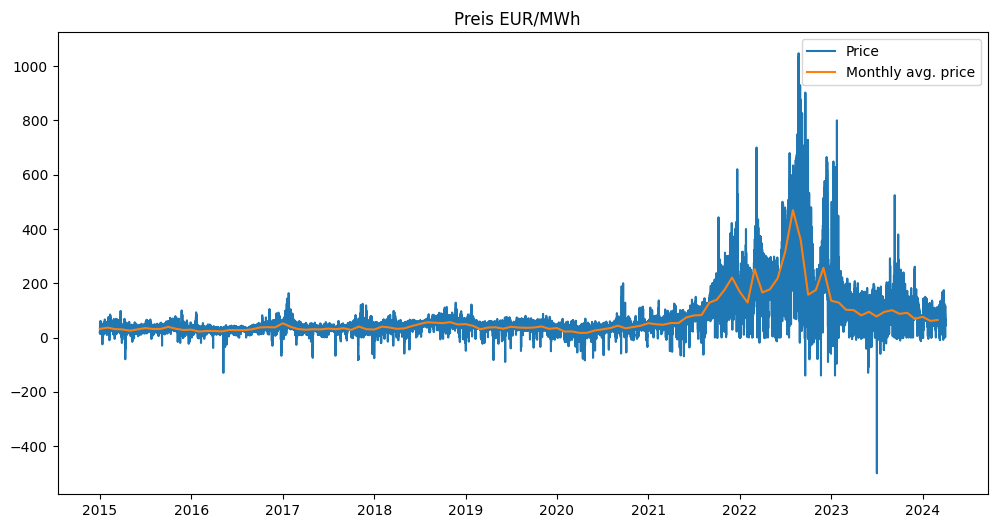
\includegraphics[keepaspectratio]{src/image.png}}
\caption{Overwiev of dayahead price development}
\end{figure}

However, at this scale, the data might not be very indicative. To gain
further insight, a simple decomposition is done on the span of the last
four weeks. Here, the seasonal window clearly shows each day, with 28
distinct repeating patterns, showcasing the individual days and
indicating a strong daily cycle. The trend window on the other hand,
indicates a lowered prices on weekends, displaying a second weekly
seasonality typical for energy data.

\begin{figure}
\centering
{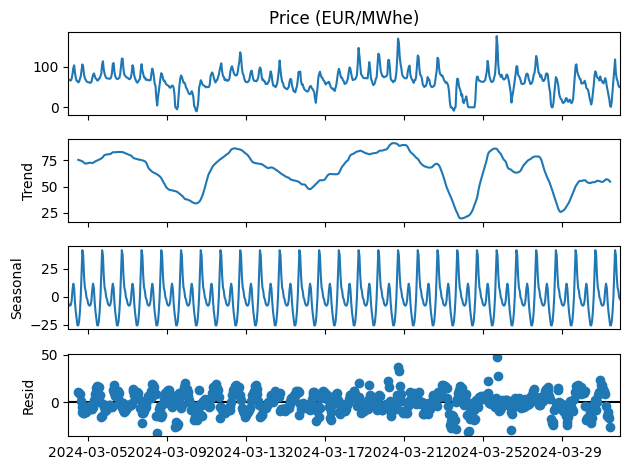
\includegraphics[keepaspectratio]{src/image-2.png}}
\caption{Decomposition of dayahead prices into seasonal patterns, trend
window and residual}
\end{figure}

A plot of the electricity price throughout the course of the day reveals
two peaks, occurring at approximately 6 a.m. and 5 p.m., respectively.
Additionally, the price reaches its lowest point during the night, at 2
a.m. This indicates a pronounced decline in energy consumption,
compensating the reduced production of energy from solar sources during
nocturnal hours. Conversely, solar production is most active between the
hours of 11 a.m. and 4 p.m.

\begin{figure}
\centering
{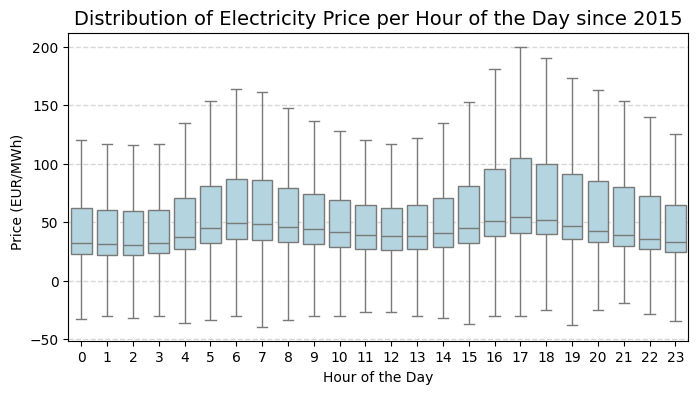
\includegraphics[keepaspectratio]{src/image-3.png}}
\caption{Distribution of electricity price per hour of the day since
2015}
\end{figure}

Secondly, let us examine the daily trend over the course of a week. By
averaging the values of the entire data set per weekday, it becomes
evident that there is a clear downward trend in prices over the weekend,
with Sunday in particular being a low point. This can be speculated to
be related to lowered consumption. This observation led us to include a
dedicated weekday field in our data to enhance the accuracy of our
prediction.

\begin{figure}
\centering
{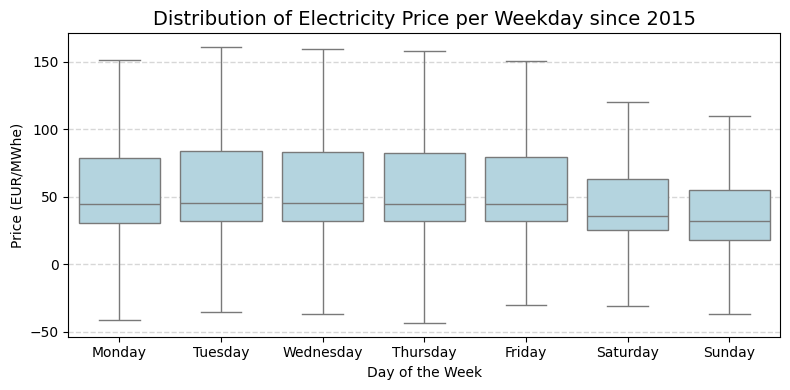
\includegraphics[keepaspectratio]{src/image-4.png}}
\caption{Distribution of electricity price per weekday since 2015}
\end{figure}

Averaging the months of the year, a further difference is visible. This
can be speculated to both pertain to temperatures and therefore heating
and weather influences.

\begin{figure}
\centering
{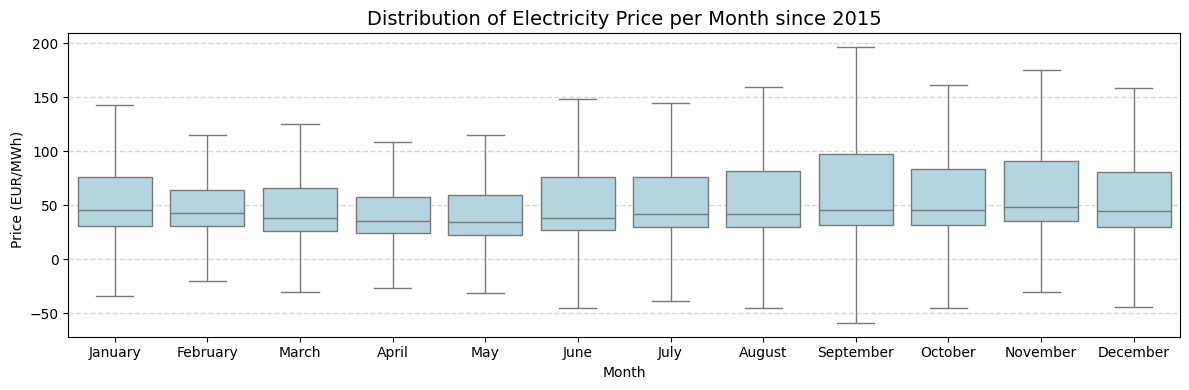
\includegraphics[keepaspectratio]{src/image-7.png}}
\caption{Distribution of electricity price per month since 2015}
\end{figure}

Averaging the individual years, a striking spike during the year 2022
stands out.

\begin{figure}
\centering
{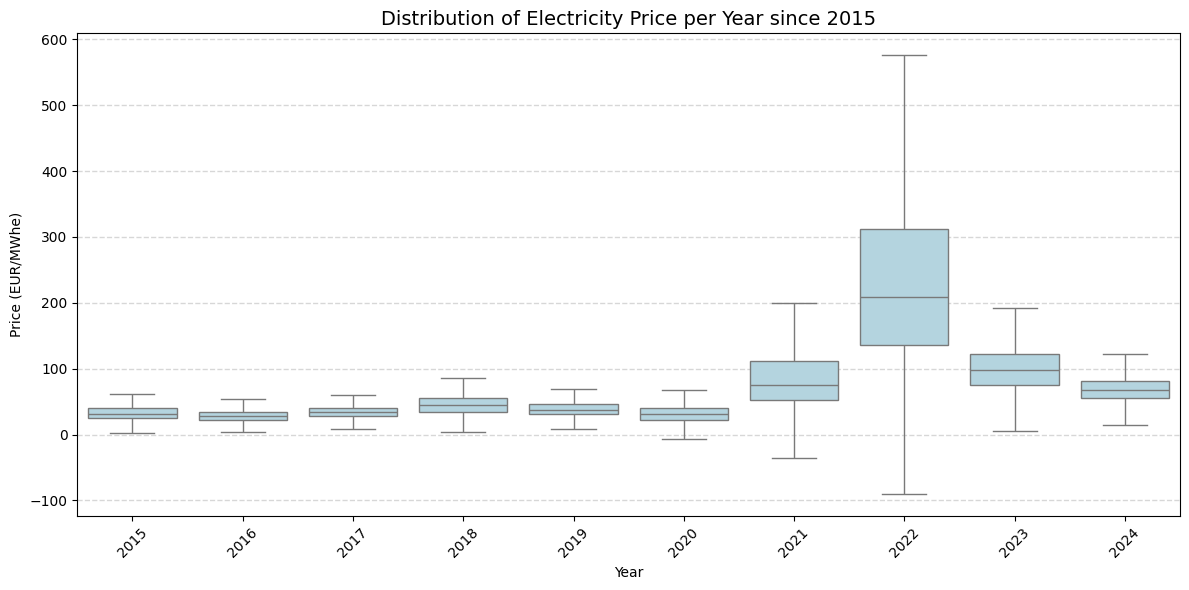
\includegraphics[keepaspectratio]{src/image-5.png}}
\caption{Distribution of electricity price per year since 2015}
\end{figure}

This might both be due to factors previously outlined at the beginning
of the section, however, that would not sufficiently explain the
reduction of prices in subsequent years. A first idea might be that a
slight increase due to inflation is to be expected, however the spike
clearly supersedes the inflation of 7,9\% that year. \hyperref[bibliography]{[Finanztools, Inflationsraten Deutschland, 2025]}

\begin{figure}
\centering
{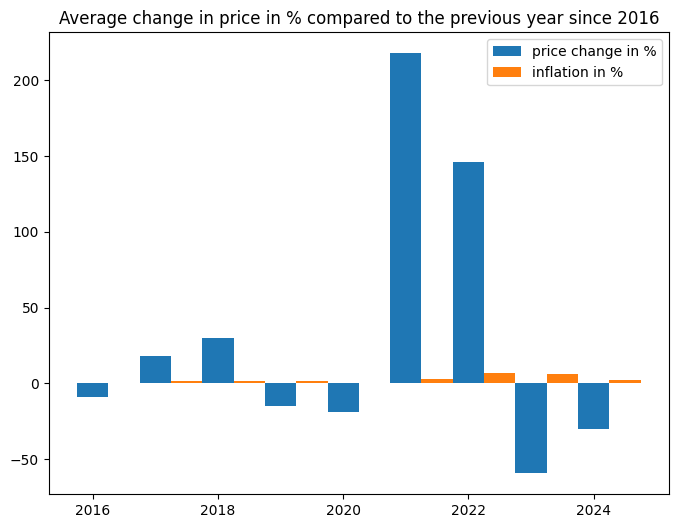
\includegraphics[keepaspectratio]{src/image-6.png}}
\caption{Average change in price compared to the previous year since
2016}
\end{figure}

It is therefore likely, that the start of Russia's invasion of Ukraine
heavily influenced the prices by driving up fossil fuel prices due to
sanctions and stop of imports. Later that year the explosions at the
Nord-Stream-Pipelines occured. These geopolitical events and their
complex interconnected ramifications also influenced prices in
neighbouring countries and thereby the intra-border flow. Inside
Germany, the shift towards renewable energy sources was accelerated and
the usage of gas heavily disincentiviced through pricing in order to
keep gas storages filled for winter, to enable Germans to continue to
heat.

    \paragraph{Feature Selection}\label{feature-selection}

An important step in the process of finding the right features to train
the model is to examine the correlation between the variables in the
given dataset. Since there are many different features, a heatmap plot
is a good way to display them all while still providing a practical
overview.

To get a more precise feature selection, the Python library pandas
provides a .corr() function which can be used to get the values
satisfying a chosen condition, e.g., getting the ten most correlating
values relating to `price'.

    \begin{tcolorbox}[breakable, size=fbox, boxrule=1pt, pad at break*=1mm,colback=cellbackground, colframe=cellborder]
\prompt{In}{incolor}{5}{\boxspacing}
\begin{small}
\begin{Verbatim}[commandchars=\\\{\}]
\PY{k+kn}{import}\PY{+w}{ }\PY{n+nn}{pandas}\PY{+w}{ }\PY{k}{as}\PY{+w}{ }\PY{n+nn}{pd}
\PY{k+kn}{import}\PY{+w}{ }\PY{n+nn}{seaborn}\PY{+w}{ }\PY{k}{as}\PY{+w}{ }\PY{n+nn}{sns}
\PY{k+kn}{import}\PY{+w}{ }\PY{n+nn}{matplotlib}\PY{n+nn}{.}\PY{n+nn}{pyplot}\PY{+w}{ }\PY{k}{as}\PY{+w}{ }\PY{n+nn}{plt}

\PY{c+c1}{\PYZsh{}loada dataframe from: /merged\PYZus{}data/data\PYZus{}collection/smard.csv}

\PY{c+c1}{\PYZsh{}for local testing: \PYZsq{}/home/user/ai\PYZhy{}project/push\PYZus{}to\PYZus{}final\PYZus{}submission/final\PYZhy{}submission//merged\PYZus{}data/data\PYZus{}collection/smard.csv\PYZsq{}}
\PY{n}{a\PYZus{}smard\PYZus{}df} \PY{o}{=} \PY{n}{pd}\PY{o}{.}\PY{n}{read\PYZus{}csv}\PY{p}{(}\PY{l+s+s1}{\PYZsq{}}\PY{l+s+s1}{merged\PYZus{}data/data\PYZus{}collection/smard.csv}\PY{l+s+s1}{\PYZsq{}}\PY{p}{)}
\PY{n}{a\PYZus{}smard\PYZus{}df}\PY{o}{=}\PY{n}{a\PYZus{}smard\PYZus{}df}\PY{p}{[}\PY{n}{a\PYZus{}smard\PYZus{}df}\PY{o}{.}\PY{n}{duplicated}\PY{p}{(}\PY{n}{keep}\PY{o}{=}\PY{k+kc}{False}\PY{p}{)} \PY{o}{==} \PY{k+kc}{False}\PY{p}{]}



\PY{c+c1}{\PYZsh{}dataslice with fewest NaN entries}
\PY{n}{a\PYZus{}smard\PYZus{}df\PYZus{}slice} \PY{o}{=} \PY{n}{a\PYZus{}smard\PYZus{}df}\PY{p}{[}\PY{p}{(}\PY{n}{pd}\PY{o}{.}\PY{n}{to\PYZus{}datetime}\PY{p}{(}\PY{n}{a\PYZus{}smard\PYZus{}df}\PY{p}{[}\PY{l+s+s1}{\PYZsq{}}\PY{l+s+s1}{Date}\PY{l+s+s1}{\PYZsq{}}\PY{p}{]}\PY{p}{)}\PY{o}{\PYZgt{}}\PY{o}{=}\PY{n}{pd}\PY{o}{.}\PY{n}{to\PYZus{}datetime}\PY{p}{(}\PY{l+s+s1}{\PYZsq{}}\PY{l+s+s1}{2022\PYZhy{}01\PYZhy{}31 00:00:00}\PY{l+s+s1}{\PYZsq{}}\PY{p}{)}\PY{p}{)} \PY{o}{\PYZam{}} 
\PY{p}{(}\PY{n}{pd}\PY{o}{.}\PY{n}{to\PYZus{}datetime}\PY{p}{(}\PY{n}{a\PYZus{}smard\PYZus{}df}\PY{p}{[}\PY{l+s+s1}{\PYZsq{}}\PY{l+s+s1}{Date}\PY{l+s+s1}{\PYZsq{}}\PY{p}{]}\PY{p}{)}\PY{o}{\PYZlt{}}\PY{o}{=}\PY{n}{pd}\PY{o}{.}\PY{n}{to\PYZus{}datetime}\PY{p}{(}\PY{l+s+s1}{\PYZsq{}}\PY{l+s+s1}{2022\PYZhy{}05\PYZhy{}31 00:00:00}\PY{l+s+s1}{\PYZsq{}}\PY{p}{)}\PY{p}{)}\PY{p}{]}

\PY{n}{a\PYZus{}smard\PYZus{}df} \PY{o}{=} \PY{n}{a\PYZus{}smard\PYZus{}df}\PY{o}{.}\PY{n}{drop}\PY{p}{(}\PY{n}{columns}\PY{o}{=}\PY{p}{[}\PY{l+s+s1}{\PYZsq{}}\PY{l+s+s1}{Date}\PY{l+s+s1}{\PYZsq{}}\PY{p}{,}\PY{l+s+s1}{\PYZsq{}}\PY{l+s+s1}{End\PYZus{}Date}\PY{l+s+s1}{\PYZsq{}}\PY{p}{]}\PY{p}{)}
\PY{n}{a\PYZus{}smard\PYZus{}df\PYZus{}slice} \PY{o}{=} \PY{n}{a\PYZus{}smard\PYZus{}df\PYZus{}slice}\PY{o}{.}\PY{n}{drop}\PY{p}{(}\PY{n}{columns}\PY{o}{=}\PY{p}{[}\PY{l+s+s1}{\PYZsq{}}\PY{l+s+s1}{Date}\PY{l+s+s1}{\PYZsq{}}\PY{p}{,}\PY{l+s+s1}{\PYZsq{}}\PY{l+s+s1}{End\PYZus{}Date}\PY{l+s+s1}{\PYZsq{}}\PY{p}{]}\PY{p}{)}

\PY{c+c1}{\PYZsh{}plot Abb. 1}
\PY{n}{a\PYZus{}smard\PYZus{}df\PYZus{}corr}\PY{o}{=}\PY{n}{a\PYZus{}smard\PYZus{}df}\PY{o}{.}\PY{n}{corr}\PY{p}{(}\PY{p}{)}

\PY{n}{plt}\PY{o}{.}\PY{n}{figure}\PY{p}{(}\PY{n}{figsize}\PY{o}{=}\PY{p}{(}\PY{l+m+mi}{12}\PY{p}{,} \PY{l+m+mi}{12}\PY{p}{)}\PY{p}{)}
\PY{n}{plt}\PY{o}{.}\PY{n}{title}\PY{p}{(}\PY{l+s+s2}{\PYZdq{}}\PY{l+s+s2}{Correlation between features (fig. 1)}\PY{l+s+s2}{\PYZdq{}}\PY{p}{)}
\PY{n}{sns}\PY{o}{.}\PY{n}{heatmap}\PY{p}{(}\PY{n}{a\PYZus{}smard\PYZus{}df\PYZus{}corr}\PY{p}{,} \PY{n}{vmin}\PY{o}{=}\PY{o}{\PYZhy{}}\PY{l+m+mi}{1}\PY{p}{,} \PY{n}{vmax}\PY{o}{=}\PY{l+m+mi}{1}\PY{p}{,} \PY{n}{center}\PY{o}{=}\PY{l+m+mi}{0}\PY{p}{,} \PY{n}{cmap}\PY{o}{=}\PY{l+s+s1}{\PYZsq{}}\PY{l+s+s1}{vlag}\PY{l+s+s1}{\PYZsq{}}\PY{p}{)}

\PY{n}{plt}\PY{o}{.}\PY{n}{show}\PY{p}{(}\PY{p}{)}
\end{Verbatim}
\end{small}
\end{tcolorbox}

    \begin{center}
    \adjustimage{max size={0.9\linewidth}{0.9\paperheight}}{output_74_0.png}
    \end{center}
    { \hspace*{\fill} \\}
    
    This already provides interesting insights into the data and the impact
of the variables. Some are shown as an almost complete white line, which
means that they do not have significant correlation with any other
variable. This can be caused by multiple reasons, e.g., the variable is
missing too many values or the variable has simply no impact on the
other ones. The more saturation the colour of a square has, the more two
variables correlate with each other. Blue implies a negative direction
(values rise/fall in opposite directions) and red a positive one (values
rise/fall in the same direction). Below in figure a) and figure b), the
different strategies ``filling with mean'' and ``filling with zero'' get
compared and visualized.

The usage of only a selected part of the data set seems to change the
correlation between the ``Price'' and the selected variable
``af\_Activation\_Price\_Minus\_MWh''. This specific variable got
further examined since it seems to be one of the most important features
in terms of correlation to the price, at least in the smard dataset. The
importance is shown in table c).

    \begin{tcolorbox}[breakable, size=fbox, boxrule=1pt, pad at break*=1mm,colback=cellbackground, colframe=cellborder]
\prompt{In}{incolor}{6}{\boxspacing}
\begin{small}
\begin{Verbatim}[commandchars=\\\{\}]
\PY{n}{mean\PYZus{}df} \PY{o}{=} \PY{n}{a\PYZus{}smard\PYZus{}df}\PY{o}{.}\PY{n}{fillna}\PY{p}{(}\PY{n}{a\PYZus{}smard\PYZus{}df}\PY{o}{.}\PY{n}{mean}\PY{p}{(}\PY{p}{)}\PY{p}{)}
\PY{n}{mean\PYZus{}df\PYZus{}slice} \PY{o}{=} \PY{n}{a\PYZus{}smard\PYZus{}df\PYZus{}slice}\PY{o}{.}\PY{n}{fillna}\PY{p}{(}\PY{n}{a\PYZus{}smard\PYZus{}df\PYZus{}slice}\PY{o}{.}\PY{n}{mean}\PY{p}{(}\PY{p}{)}\PY{p}{)}

\PY{n}{zero\PYZus{}df} \PY{o}{=} \PY{n}{a\PYZus{}smard\PYZus{}df}\PY{o}{.}\PY{n}{apply}\PY{p}{(}\PY{k}{lambda} \PY{n}{col}\PY{p}{:} \PY{n}{col}\PY{o}{.}\PY{n}{fillna}\PY{p}{(}\PY{l+m+mi}{0}\PY{p}{)}\PY{p}{,} \PY{n}{axis}\PY{o}{=}\PY{l+m+mi}{0}\PY{p}{)}
\PY{n}{zero\PYZus{}df\PYZus{}slice} \PY{o}{=} \PY{n}{a\PYZus{}smard\PYZus{}df\PYZus{}slice}\PY{o}{.}\PY{n}{apply}\PY{p}{(}\PY{k}{lambda} \PY{n}{col}\PY{p}{:} \PY{n}{col}\PY{o}{.}\PY{n}{fillna}\PY{p}{(}\PY{l+m+mi}{0}\PY{p}{)}\PY{p}{,} \PY{n}{axis}\PY{o}{=}\PY{l+m+mi}{0}\PY{p}{)}

\PY{n}{plt}\PY{o}{.}\PY{n}{scatter}\PY{p}{(}\PY{n}{x} \PY{o}{=} \PY{n}{mean\PYZus{}df}\PY{p}{[}\PY{l+s+s1}{\PYZsq{}}\PY{l+s+s1}{af\PYZus{}Activation\PYZus{}Price\PYZus{}Minus\PYZus{}EUR\PYZus{}MWh}\PY{l+s+s1}{\PYZsq{}}\PY{p}{]}\PY{p}{,} \PY{n}{y} \PY{o}{=} \PY{n}{mean\PYZus{}df}\PY{p}{[}\PY{l+s+s1}{\PYZsq{}}\PY{l+s+s1}{Price\PYZus{}Calculated\PYZus{}EUR\PYZus{}MWh}\PY{l+s+s1}{\PYZsq{}}\PY{p}{]}\PY{p}{,} \PY{n}{color}\PY{o}{=}\PY{l+s+s1}{\PYZsq{}}\PY{l+s+s1}{blue}\PY{l+s+s1}{\PYZsq{}}\PY{p}{,} \PY{n}{alpha}\PY{o}{=}\PY{l+m+mf}{0.4}\PY{p}{,} \PY{n}{label}\PY{o}{=}\PY{l+s+s1}{\PYZsq{}}\PY{l+s+s1}{mean}\PY{l+s+s1}{\PYZsq{}}\PY{p}{)}
\PY{n}{plt}\PY{o}{.}\PY{n}{scatter}\PY{p}{(}\PY{n}{x} \PY{o}{=} \PY{n}{zero\PYZus{}df}\PY{p}{[}\PY{l+s+s1}{\PYZsq{}}\PY{l+s+s1}{af\PYZus{}Activation\PYZus{}Price\PYZus{}Minus\PYZus{}EUR\PYZus{}MWh}\PY{l+s+s1}{\PYZsq{}}\PY{p}{]}\PY{p}{,} \PY{n}{y} \PY{o}{=} \PY{n}{zero\PYZus{}df}\PY{p}{[}\PY{l+s+s1}{\PYZsq{}}\PY{l+s+s1}{Price\PYZus{}Calculated\PYZus{}EUR\PYZus{}MWh}\PY{l+s+s1}{\PYZsq{}}\PY{p}{]}\PY{p}{,} \PY{n}{color}\PY{o}{=}\PY{l+s+s1}{\PYZsq{}}\PY{l+s+s1}{green}\PY{l+s+s1}{\PYZsq{}}\PY{p}{,} \PY{n}{alpha}\PY{o}{=}\PY{l+m+mf}{0.4}\PY{p}{,} \PY{n}{label}\PY{o}{=}\PY{l+s+s1}{\PYZsq{}}\PY{l+s+s1}{zero}\PY{l+s+s1}{\PYZsq{}}\PY{p}{)}

\PY{n}{plt}\PY{o}{.}\PY{n}{xlabel}\PY{p}{(}\PY{l+s+s2}{\PYZdq{}}\PY{l+s+s2}{af\PYZus{}Activation\PYZus{}Price\PYZus{}Minus\PYZus{}EUR\PYZus{}MWh}\PY{l+s+s2}{\PYZdq{}}\PY{p}{)}
\PY{n}{plt}\PY{o}{.}\PY{n}{ylabel}\PY{p}{(}\PY{l+s+s2}{\PYZdq{}}\PY{l+s+s2}{Price\PYZus{}Calculated\PYZus{}EUR\PYZus{}MWh}\PY{l+s+s2}{\PYZdq{}}\PY{p}{)}
\PY{n}{plt}\PY{o}{.}\PY{n}{legend}\PY{p}{(}\PY{p}{)}
\PY{n}{plt}\PY{o}{.}\PY{n}{title}\PY{p}{(}\PY{l+s+s2}{\PYZdq{}}\PY{l+s+s2}{Correlation if NaN is filled with mean/zero on the complete time frame; fig. a)}\PY{l+s+s2}{\PYZdq{}}\PY{p}{)}
\PY{n}{plt}\PY{o}{.}\PY{n}{show}\PY{p}{(}\PY{p}{)}
\end{Verbatim}
\end{small}
\end{tcolorbox}

    \begin{center}
    \adjustimage{max size={0.9\linewidth}{0.9\paperheight}}{output_76_0.png}
    \end{center}
    { \hspace*{\fill} \\}
    
    \begin{tcolorbox}[breakable, size=fbox, boxrule=1pt, pad at break*=1mm,colback=cellbackground, colframe=cellborder]
\prompt{In}{incolor}{7}{\boxspacing}
\begin{small}
\begin{Verbatim}[commandchars=\\\{\}]
\PY{n}{plt}\PY{o}{.}\PY{n}{scatter}\PY{p}{(}\PY{n}{x} \PY{o}{=} \PY{n}{mean\PYZus{}df\PYZus{}slice}\PY{p}{[}\PY{l+s+s1}{\PYZsq{}}\PY{l+s+s1}{af\PYZus{}Activation\PYZus{}Price\PYZus{}Minus\PYZus{}EUR\PYZus{}MWh}\PY{l+s+s1}{\PYZsq{}}\PY{p}{]}\PY{p}{,} \PY{n}{y} \PY{o}{=} \PY{n}{mean\PYZus{}df\PYZus{}slice}\PY{p}{[}\PY{l+s+s1}{\PYZsq{}}\PY{l+s+s1}{Price\PYZus{}Calculated\PYZus{}EUR\PYZus{}MWh}\PY{l+s+s1}{\PYZsq{}}\PY{p}{]}\PY{p}{,} \PY{n}{color}\PY{o}{=}\PY{l+s+s1}{\PYZsq{}}\PY{l+s+s1}{blue}\PY{l+s+s1}{\PYZsq{}}\PY{p}{,} \PY{n}{alpha}\PY{o}{=}\PY{l+m+mf}{0.4}\PY{p}{,} \PY{n}{label}\PY{o}{=}\PY{l+s+s1}{\PYZsq{}}\PY{l+s+s1}{mean}\PY{l+s+s1}{\PYZsq{}}\PY{p}{)}
\PY{n}{plt}\PY{o}{.}\PY{n}{scatter}\PY{p}{(}\PY{n}{x} \PY{o}{=} \PY{n}{zero\PYZus{}df\PYZus{}slice}\PY{p}{[}\PY{l+s+s1}{\PYZsq{}}\PY{l+s+s1}{af\PYZus{}Activation\PYZus{}Price\PYZus{}Minus\PYZus{}EUR\PYZus{}MWh}\PY{l+s+s1}{\PYZsq{}}\PY{p}{]}\PY{p}{,} \PY{n}{y} \PY{o}{=} \PY{n}{zero\PYZus{}df\PYZus{}slice}\PY{p}{[}\PY{l+s+s1}{\PYZsq{}}\PY{l+s+s1}{Price\PYZus{}Calculated\PYZus{}EUR\PYZus{}MWh}\PY{l+s+s1}{\PYZsq{}}\PY{p}{]}\PY{p}{,} \PY{n}{color}\PY{o}{=}\PY{l+s+s1}{\PYZsq{}}\PY{l+s+s1}{green}\PY{l+s+s1}{\PYZsq{}}\PY{p}{,} \PY{n}{alpha}\PY{o}{=}\PY{l+m+mf}{0.4}\PY{p}{,} \PY{n}{label}\PY{o}{=}\PY{l+s+s1}{\PYZsq{}}\PY{l+s+s1}{zero}\PY{l+s+s1}{\PYZsq{}}\PY{p}{)}

\PY{n}{plt}\PY{o}{.}\PY{n}{xlabel}\PY{p}{(}\PY{l+s+s2}{\PYZdq{}}\PY{l+s+s2}{af\PYZus{}Activation\PYZus{}Price\PYZus{}Minus\PYZus{}EUR\PYZus{}MWh}\PY{l+s+s2}{\PYZdq{}}\PY{p}{)}
\PY{n}{plt}\PY{o}{.}\PY{n}{ylabel}\PY{p}{(}\PY{l+s+s2}{\PYZdq{}}\PY{l+s+s2}{Price\PYZus{}Calculated\PYZus{}EUR\PYZus{}MWh}\PY{l+s+s2}{\PYZdq{}}\PY{p}{)}
\PY{n}{plt}\PY{o}{.}\PY{n}{legend}\PY{p}{(}\PY{p}{)}
\PY{n}{plt}\PY{o}{.}\PY{n}{title}\PY{p}{(}\PY{l+s+s2}{\PYZdq{}}\PY{l+s+s2}{Correlation if NaN is filled with mean/zero for a smaller selected time frame; fig b)}\PY{l+s+s2}{\PYZdq{}}\PY{p}{)}
\PY{n}{plt}\PY{o}{.}\PY{n}{show}\PY{p}{(}\PY{p}{)}
\end{Verbatim}
\end{small}
\end{tcolorbox}

    \begin{center}
    \adjustimage{max size={0.9\linewidth}{0.9\paperheight}}{output_77_0.png}
    \end{center}
    { \hspace*{\fill} \\}
    
    Another method to compare the two methods is to print out the variables
with the highest correlation after the corresponding changes to the
dataset. This comparison was made on the complete time frame. The
following table shows which variables have the highest correlation with
the variable ``Price\_Calculated\_EUR\_MWh''.

Table c)

\rowcolors{2}{white}{gray!25}
{\fontsize{8pt}{10pt}\selectfont\begin{longtable}[]{@{}
  >{\raggedright\arraybackslash}p{(\linewidth - 6\tabcolsep) * \real{0.1528}}
  >{\raggedright\arraybackslash}p{(\linewidth - 6\tabcolsep) * \real{0.2500}}
  >{\raggedright\arraybackslash}p{(\linewidth - 6\tabcolsep) * \real{0.2917}}
  >{\raggedright\arraybackslash}p{(\linewidth - 6\tabcolsep) * \real{0.3056}}@{}}
\toprule\noalign{}
\begin{minipage}[b]{\linewidth}\raggedright
Ranking (descending)
\end{minipage} & \begin{minipage}[b]{\linewidth}\raggedright
Dataset with NaN values
\end{minipage} & \begin{minipage}[b]{\linewidth}\raggedright
Dataset with NaN values replaced by mean
\end{minipage} & \begin{minipage}[b]{\linewidth}\raggedright
Dataset with NaN values replaced by 0
\end{minipage} \\
\midrule\noalign{}
\endhead
\bottomrule\noalign{}
\endlastfoot
1 &
af\_\hspace{0pt}Activation\_\hspace{0pt}Price\_\hspace{0pt}Plus\_\hspace{0pt}EUR\_\hspace{0pt}MWh
&
af\_\hspace{0pt}Activation\_\hspace{0pt}Price\_\hspace{0pt}Plus\_\hspace{0pt}EUR\_\hspace{0pt}MWh
& Net\_\hspace{0pt}Income\_\hspace{0pt}EUR \\
2 &
af\_\hspace{0pt}Activation\_\hspace{0pt}Price\_\hspace{0pt}Minus\_\hspace{0pt}EUR\_\hspace{0pt}MWh
& Net\_\hspace{0pt}Income\_\hspace{0pt}EUR &
Balancing\_\hspace{0pt}Services\_\hspace{0pt}Calculated\_\hspace{0pt}EUR \\
3 &
mf\_\hspace{0pt}Activation\_\hspace{0pt}Price\_\hspace{0pt}Plus\_\hspace{0pt}EUR\_\hspace{0pt}MWh
&
af\_\hspace{0pt}Activation\_\hspace{0pt}Price\_\hspace{0pt}Minus\_\hspace{0pt}EUR\_\hspace{0pt}MWh
& E\_\hspace{0pt}NorwayImport\_\hspace{0pt}MWh \\
4 & Net\_\hspace{0pt}Income\_\hspace{0pt}EUR &
af\_\hspace{0pt}E\_\hspace{0pt}Volume\_\hspace{0pt}Activated\_\hspace{0pt}Minus\_\hspace{0pt}MWh
&
E\_\hspace{0pt}NorwayImport\_\hspace{0pt}corssBorderPhysical\_\hspace{0pt}MWh \\
\end{longtable}}

The results show that the choice between filling with zero or filling
with the mean can have an impact on the data.

However, more significant is the difference between the usage of a
certain smaller section containing much less empty values instead of
just using everything that is available. Therefore, the priority should
be to use less but complete data instead of a dataset with big gaps.

    \subsection{Comparing Feature
Importances}\label{comparing-feature-importances}

Since our data collection resulted in 157 features, the influence each
data point has on the final prediction is unknown. In this part of the
report, different methods of calculating these feature importances are
presented with their results.

\paragraph{AutoGluon}\label{autogluon}

To find out which features AutoGluon focuses on, the final AutoGluon
model was analyzed using Permutation Feature Importance. Feature
importance is calculated by shuffling the values of a feature and
observing whether the model's performance declines. In the plot below,
the feature importance of the best model is shown. The values for
importance are uncharacteristically low and do not provide an accurate
view of the actual feature importance in our model, as only one of the
various models in the ensemble can use all of the features.

    \begin{tcolorbox}[breakable, size=fbox, boxrule=1pt, pad at break*=1mm,colback=cellbackground, colframe=cellborder]
\prompt{In}{incolor}{4}{\boxspacing}
\begin{small}
\begin{Verbatim}[commandchars=\\\{\}]
\PY{k+kn}{import}\PY{+w}{ }\PY{n+nn}{pandas}\PY{+w}{ }\PY{k}{as}\PY{+w}{ }\PY{n+nn}{pd}
\PY{k+kn}{import}\PY{+w}{ }\PY{n+nn}{matplotlib}\PY{n+nn}{.}\PY{n+nn}{pyplot}\PY{+w}{ }\PY{k}{as}\PY{+w}{ }\PY{n+nn}{plt}

\PY{c+c1}{\PYZsh{} Load the CSV file}
\PY{n}{file\PYZus{}path} \PY{o}{=} \PY{l+s+s2}{\PYZdq{}}\PY{l+s+s2}{temp/feature\PYZus{}importance.csv}\PY{l+s+s2}{\PYZdq{}}
\PY{n}{df} \PY{o}{=} \PY{n}{pd}\PY{o}{.}\PY{n}{read\PYZus{}csv}\PY{p}{(}\PY{n}{file\PYZus{}path}\PY{p}{)}

\PY{c+c1}{\PYZsh{} Sort the DataFrame by \PYZsq{}importance\PYZsq{} from lowest to highest}
\PY{n}{df} \PY{o}{=} \PY{n}{df}\PY{o}{.}\PY{n}{sort\PYZus{}values}\PY{p}{(}\PY{n}{by}\PY{o}{=}\PY{l+s+s1}{\PYZsq{}}\PY{l+s+s1}{importance}\PY{l+s+s1}{\PYZsq{}}\PY{p}{)}

\PY{c+c1}{\PYZsh{} Set up the figure and axes}
\PY{n}{plt}\PY{o}{.}\PY{n}{figure}\PY{p}{(}\PY{n}{figsize}\PY{o}{=}\PY{p}{(}\PY{l+m+mi}{12}\PY{p}{,} \PY{l+m+mi}{6}\PY{p}{)}\PY{p}{)}

\PY{c+c1}{\PYZsh{} Determine colors: red for negative values, blue for positive values}
\PY{n}{colors} \PY{o}{=} \PY{p}{[}\PY{l+s+s1}{\PYZsq{}}\PY{l+s+s1}{red}\PY{l+s+s1}{\PYZsq{}} \PY{k}{if} \PY{n}{val} \PY{o}{\PYZlt{}} \PY{l+m+mi}{0} \PY{k}{else} \PY{l+s+s1}{\PYZsq{}}\PY{l+s+s1}{blue}\PY{l+s+s1}{\PYZsq{}} \PY{k}{for} \PY{n}{val} \PY{o+ow}{in} \PY{n}{df}\PY{p}{[}\PY{l+s+s1}{\PYZsq{}}\PY{l+s+s1}{importance}\PY{l+s+s1}{\PYZsq{}}\PY{p}{]}\PY{p}{]}

\PY{c+c1}{\PYZsh{} Plot the \PYZsq{}importance\PYZsq{} column with the first column as x labels}
\PY{n}{plt}\PY{o}{.}\PY{n}{bar}\PY{p}{(}\PY{n}{df}\PY{o}{.}\PY{n}{iloc}\PY{p}{[}\PY{p}{:}\PY{p}{,} \PY{l+m+mi}{0}\PY{p}{]}\PY{p}{,} \PY{n}{df}\PY{p}{[}\PY{l+s+s1}{\PYZsq{}}\PY{l+s+s1}{importance}\PY{l+s+s1}{\PYZsq{}}\PY{p}{]}\PY{p}{,} \PY{n}{color}\PY{o}{=}\PY{n}{colors}\PY{p}{,} \PY{n}{alpha}\PY{o}{=}\PY{l+m+mf}{0.7}\PY{p}{)}

\PY{c+c1}{\PYZsh{} Set labels and title}
\PY{n}{plt}\PY{o}{.}\PY{n}{xlabel}\PY{p}{(}\PY{l+s+s1}{\PYZsq{}}\PY{l+s+s1}{Variable}\PY{l+s+s1}{\PYZsq{}}\PY{p}{)}
\PY{n}{plt}\PY{o}{.}\PY{n}{ylabel}\PY{p}{(}\PY{l+s+s1}{\PYZsq{}}\PY{l+s+s1}{Importance}\PY{l+s+s1}{\PYZsq{}}\PY{p}{)}
\PY{n}{plt}\PY{o}{.}\PY{n}{title}\PY{p}{(}\PY{l+s+s1}{\PYZsq{}}\PY{l+s+s1}{Feature Importance}\PY{l+s+s1}{\PYZsq{}}\PY{p}{)}

\PY{c+c1}{\PYZsh{} Rotate the x labels for better readability}
\PY{n}{plt}\PY{o}{.}\PY{n}{xticks}\PY{p}{(}\PY{n}{rotation}\PY{o}{=}\PY{l+m+mi}{90}\PY{p}{,} \PY{n}{ha}\PY{o}{=}\PY{l+s+s1}{\PYZsq{}}\PY{l+s+s1}{right}\PY{l+s+s1}{\PYZsq{}}\PY{p}{)}

\PY{c+c1}{\PYZsh{} Adjust layout to avoid overlap}
\PY{n}{plt}\PY{o}{.}\PY{n}{tight\PYZus{}layout}\PY{p}{(}\PY{p}{)}

\PY{c+c1}{\PYZsh{} Show the plot}
\PY{n}{plt}\PY{o}{.}\PY{n}{show}\PY{p}{(}\PY{p}{)}
\end{Verbatim}
\end{small}
\end{tcolorbox}

    \begin{center}
    \adjustimage{max size={0.9\linewidth}{0.9\paperheight}}{output_80_0.png}
    \end{center}
    { \hspace*{\fill} \\}
    
    \paragraph{Temporal Fusion
Transformer}\label{temporal-fusion-transformer}

We used Temporal Fusion Transformers (TFT) to gain deeper insights. TFT
is a transformer-based architecture that has the advantage of being
inherently explainable. For example, it enables the consideration of
time-series data in multiple formats while identifying the most relevant
features for forecasting. Specifically, it allows for the inclusion of
past-only features (unknown covariates) such as stock data, where future
values are unavailable; known covariates, like the day of the week,
where future values are predetermined; and static covariates, which
remain constant throughout the time series. It does this by using an
encoder to encode past-only variables and static covariates into a
format that a decoder can process together with the known covariates.
For each of those 2 components the feature importance is calculated for
each feature. To demonstrate this and evaluate our data, we consider a
selection of features from our collected data we think could be of great
importance for forecasting. Then, we train a standard TFT model to
forecast the day-ahead energy prices while considering those features.
The results are presented in the figures below. As can be seen in the
first figure containing the encoder importances (unknown covariates),
today's electricity price has the greatest influence on tomorrow's
electricity price, which is expected given its direct temporal
dependency. Among the five most important features, four are related to
wind speed, suggesting that wind energy significantly influences energy
prices by potentially providing large amounts of low-cost energy on
certain days, thereby increasing supply and reducing costs. Most of the
remaining features are roughly of similar importance. We can not say yet
if all of those features significantly impact the outcome or whether
this might be a characteristic of TFT as neural networks like TFT often
tend to consider every input variable to some degree even though it
might not provide useable information to the model. In the second figure
containing the decoder feature importances, one can see that the gas
price has surprisingly the largest impact; this could be due to
substantial increases in the gas prices in recent years due to sanctions
as a consequence of the Russo-Ukrainian War. The second most important
feature to the decoder is the forecasted load (fsctd\_load), which
indicates how much demand is expected for the following day. As we can
see here are seemingly more features of greater importance to the
decoder, with 16 features having a greater importance than two percent.
This indicates that known covariates might be of greater help to models
like TFT, likely due to their increased informational content.

    \begin{figure}
\centering
{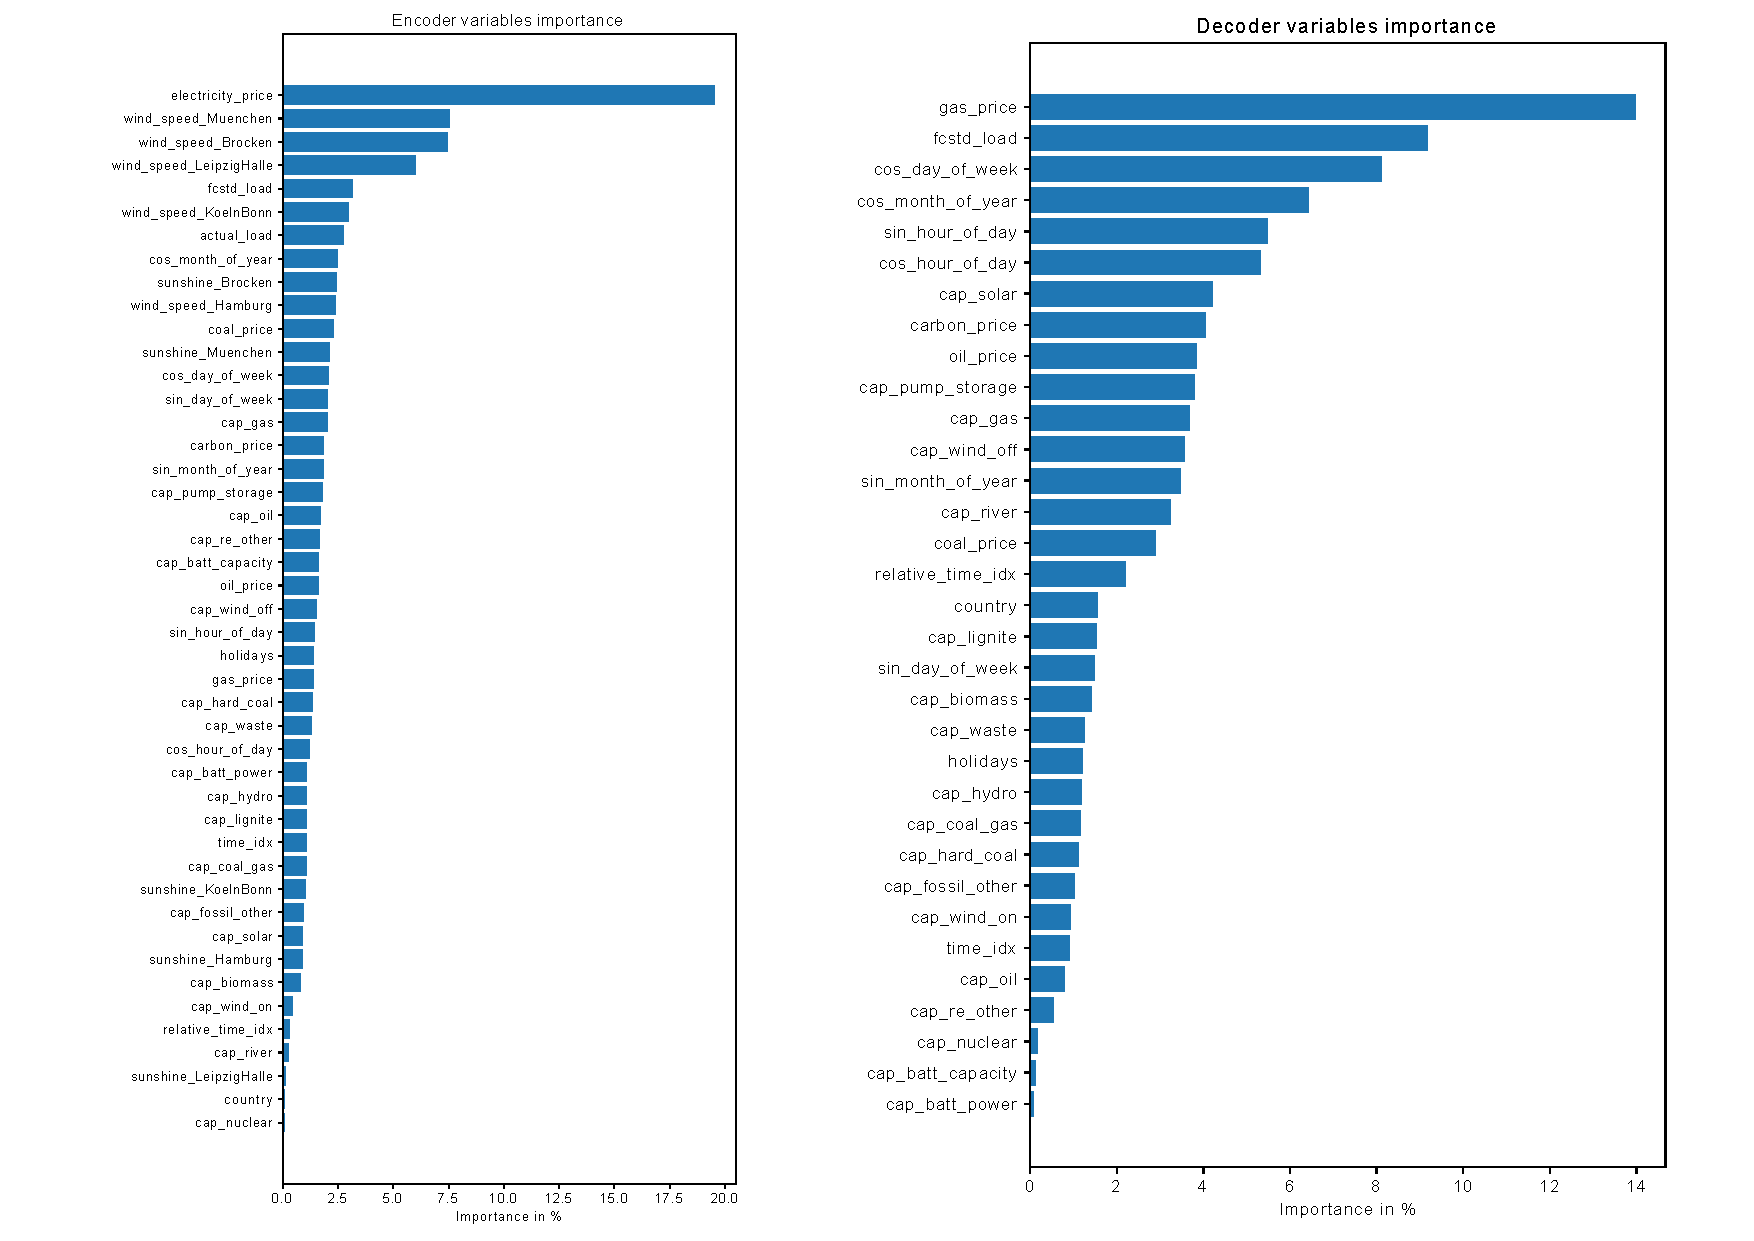
\includegraphics[keepaspectratio]{src/encoder_decoder_feat_imp.pdf}}
\caption{Feature importance calculated for the encoder and decoder
components of the TFT model}
\end{figure}

    \subparagraph{Partial Dependency
Analysis}\label{partial-dependency-analysis}

Partial Dependency Plots (PDPs) help visualise the influence of
individual features on a model's predictions. They work by averaging the
model output over different values of a particular feature, while
holding all other features constant.

    \begin{figure}
\centering
{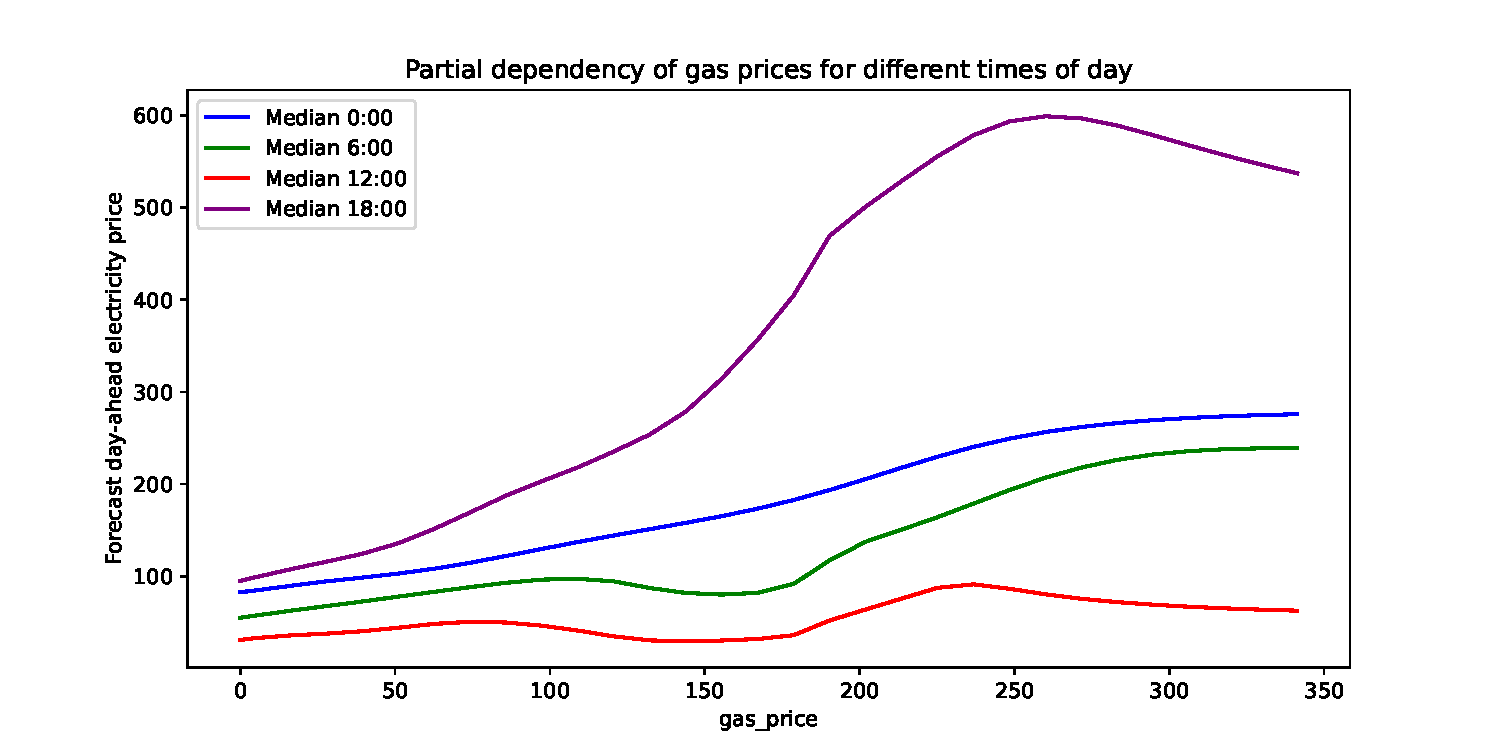
\includegraphics[keepaspectratio]{src/tft_pdp_gas_price.pdf}}
\caption{Partial Dependency Plot showing the effect of gas prices on
predicted day-ahead electricity prices at different times of the day}
\end{figure}

    The PDPs focus on four features corresponding to the TFT model. Forecast
Load (MW) is the expected electricity demand, while Day of Week,
captured by a cosine function, reflects cyclical patterns. Gas Price
(EUR/MWh) is the cost of natural gas, and Solar Generation (MW) is the
actual electricity generation from photovoltaic (PV) sources. Each PDP
shows the average predicted electricity price for different values, with
shaded areas indicating the interquartile range (IQR).

The PDP shows a strong positive correlation between gas and electricity
prices. The relationship is approximately linear, indicating that as gas
prices increase, electricity prices also increase due to higher
generation costs. Higher gas prices lead to a slight flattening of the
rate of increase, suggesting mitigating factors like switching to
alternative energy sources or demand reduction. A detailed PDP analysis
shows that the impact of gas prices on electricity prices depends on the
time of day. Electricity prices are higher during peak demand hours
(12:00 and 18:00) than at night (0:00 and 6:00). This suggests gas
prices affect electricity prices more at high demand, probably because
gas-fired power plants are used more.

    \begin{figure}
\centering
{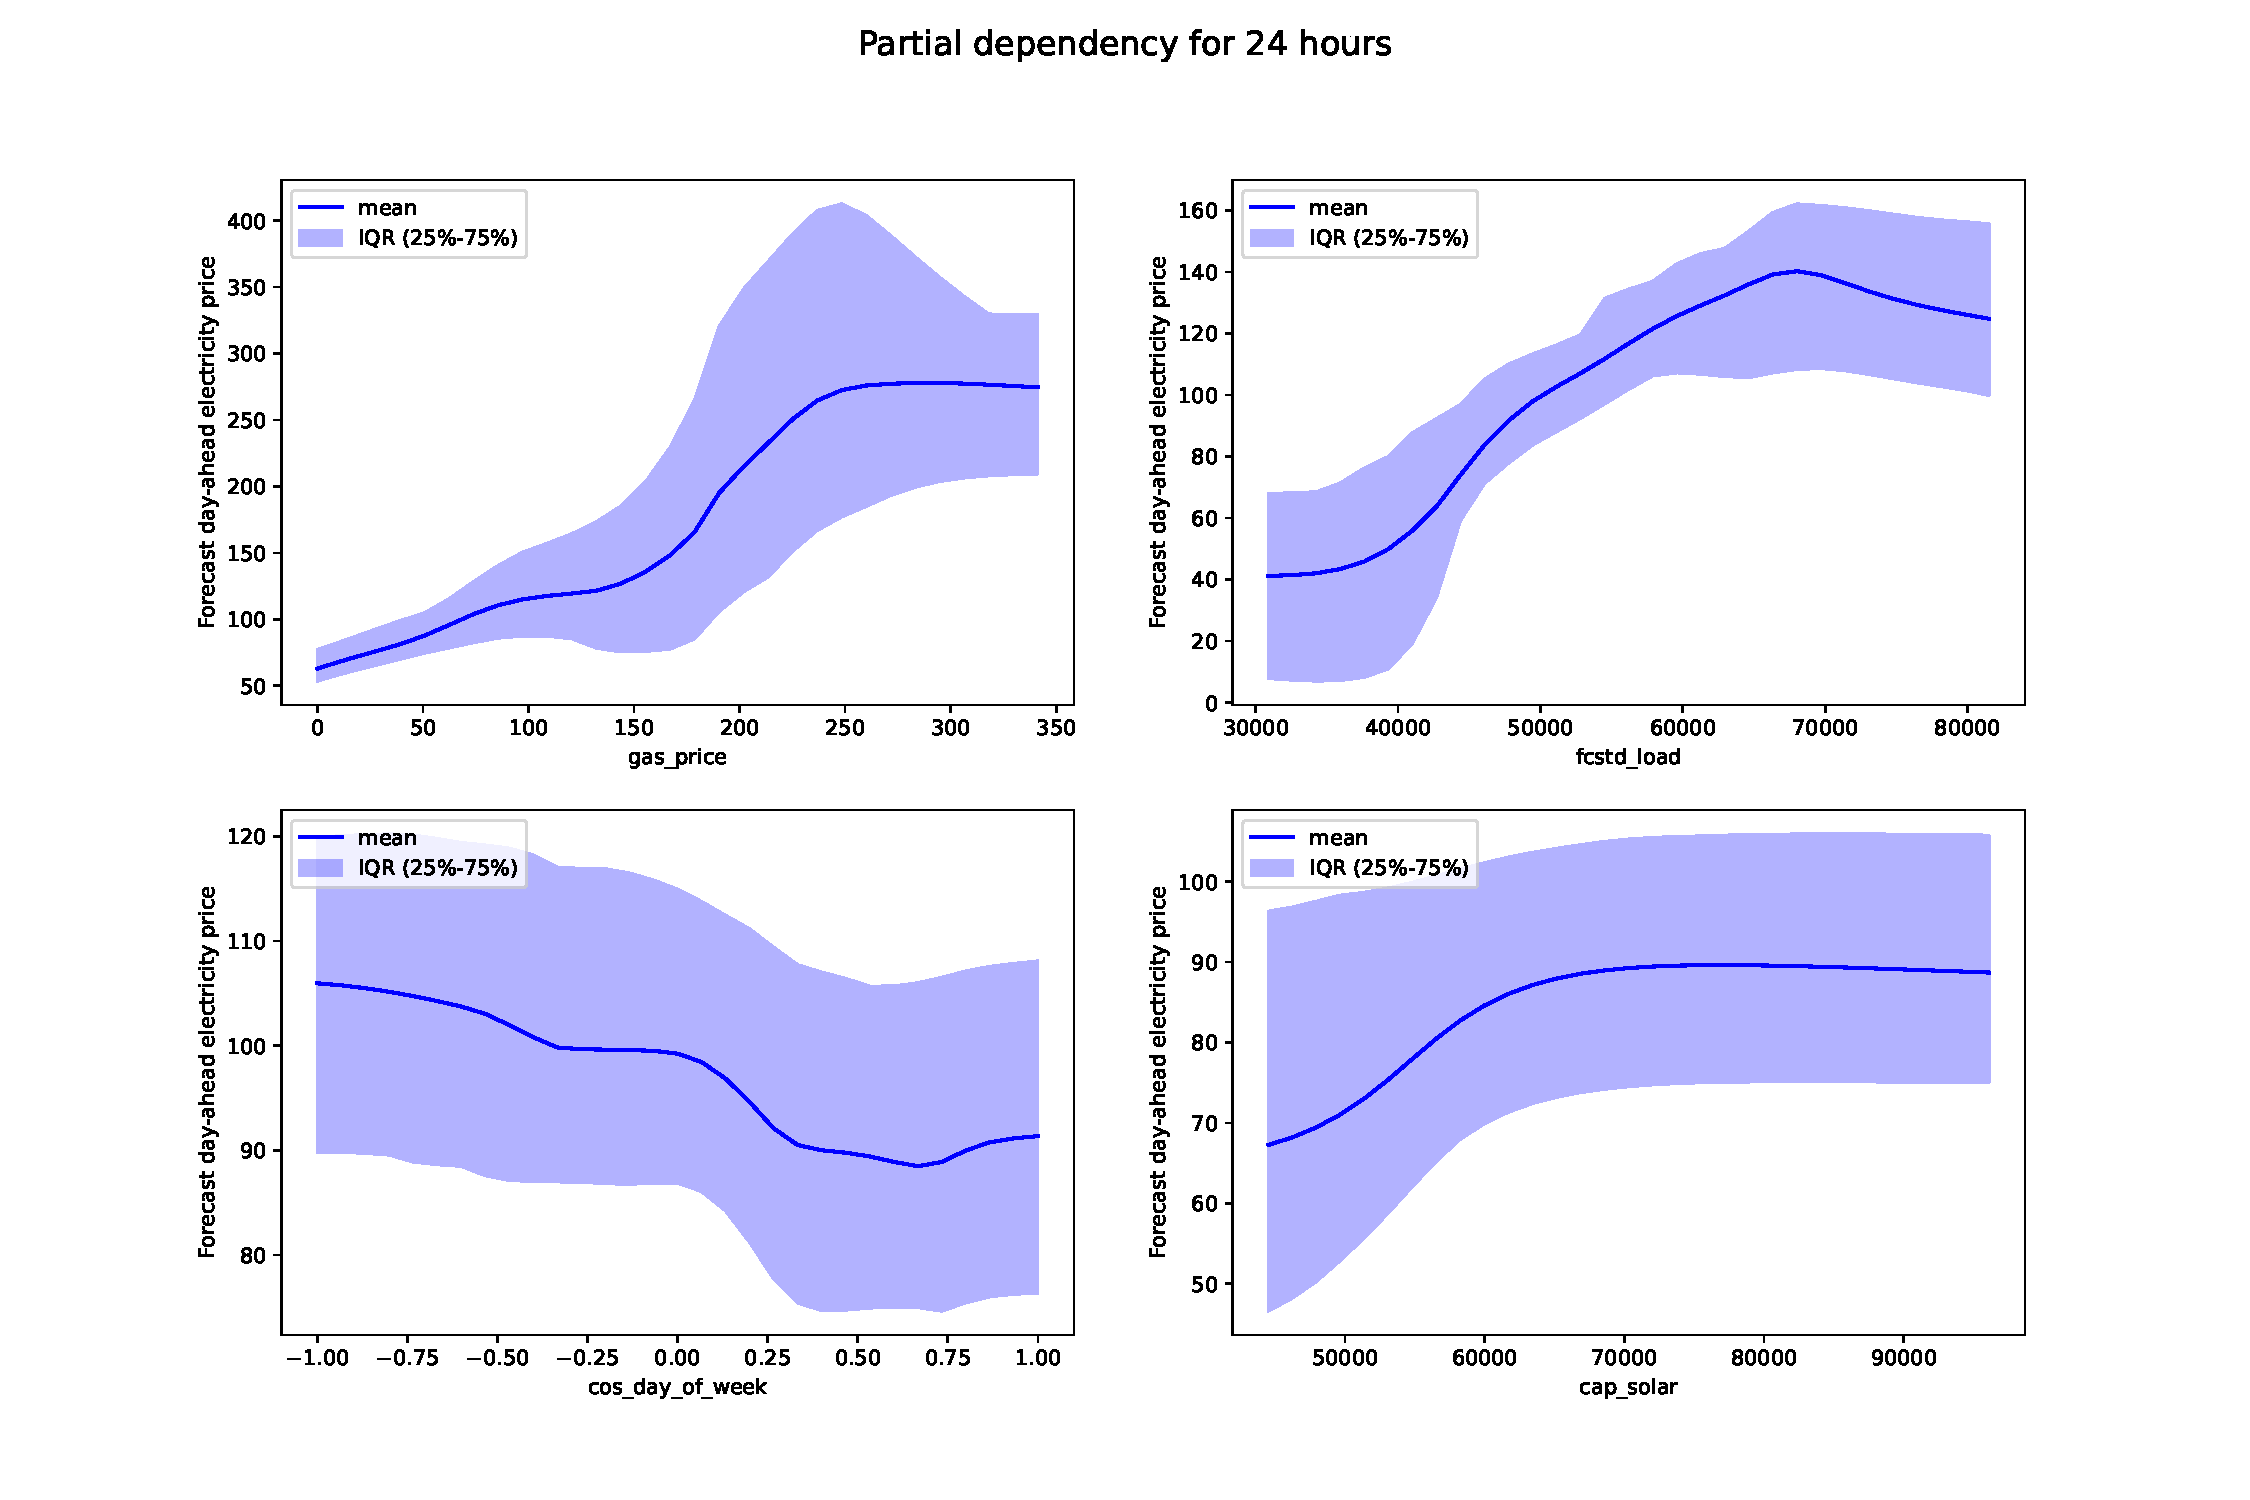
\includegraphics[keepaspectratio]{src/tft_pdp_all_hours.pdf}}
\caption{Partial Dependency Plots for the TFT model showing the impact
of forecasted load, day of the week, gas price, and solar generation on
predicted day-ahead electricity prices}
\end{figure}

    There is a positive correlation between projected electricity demand and
projected prices, with the largest price increases occurring at lower
levels of demand. As demand continues to rise, the impact on price
growth diminishes, suggesting potential saturation effects. The IQR is
wider at medium demand levels, indicating that factors such as renewable
generation and fuel costs may influence price variability.

The PDP for the day of the week shows a cyclical pattern, with lower
prices on weekends and higher prices on weekdays, driven by industrial
load fluctuations. Price variability over hours remains stable,
reflecting consistent weekly trends.

There is a clear negative relationship between solar generation and
prices. Prices fall sharply as solar generation increases, particularly
at low to medium levels, but the decline slows at very high generation
levels, possibly due to market saturation or price floors. The IQR
remains stable, indicating a predictable and consistent price impact of
solar generation across different hours.

The PDP analysis reveals the main drivers of electricity price
forecasts: gas prices and demand have a positive impact on prices, while
solar generation reduces them. The time-dependent gas price effect
highlights the importance of peak-hour dynamics.

    \subparagraph{Temporal Patterns}\label{temporal-patterns}

Besides feature importance, TFT is designed to facilitate the analysis
of its attention mechanism, enabling the identification of important
temporal patterns. The attention of our TFT is visualized in the figure
below. As seen there, TFT primarily focuses on the last 24 hours,
suggesting that daily seasonal patterns may be the most influential.
However, three minor spikes appear at 75h, 100h, and 150h, suggesting
that incorporating a longer past horizon provides valuable information
and that limiting it to only 24 hours may not be optimal.

    \begin{figure}
\centering
{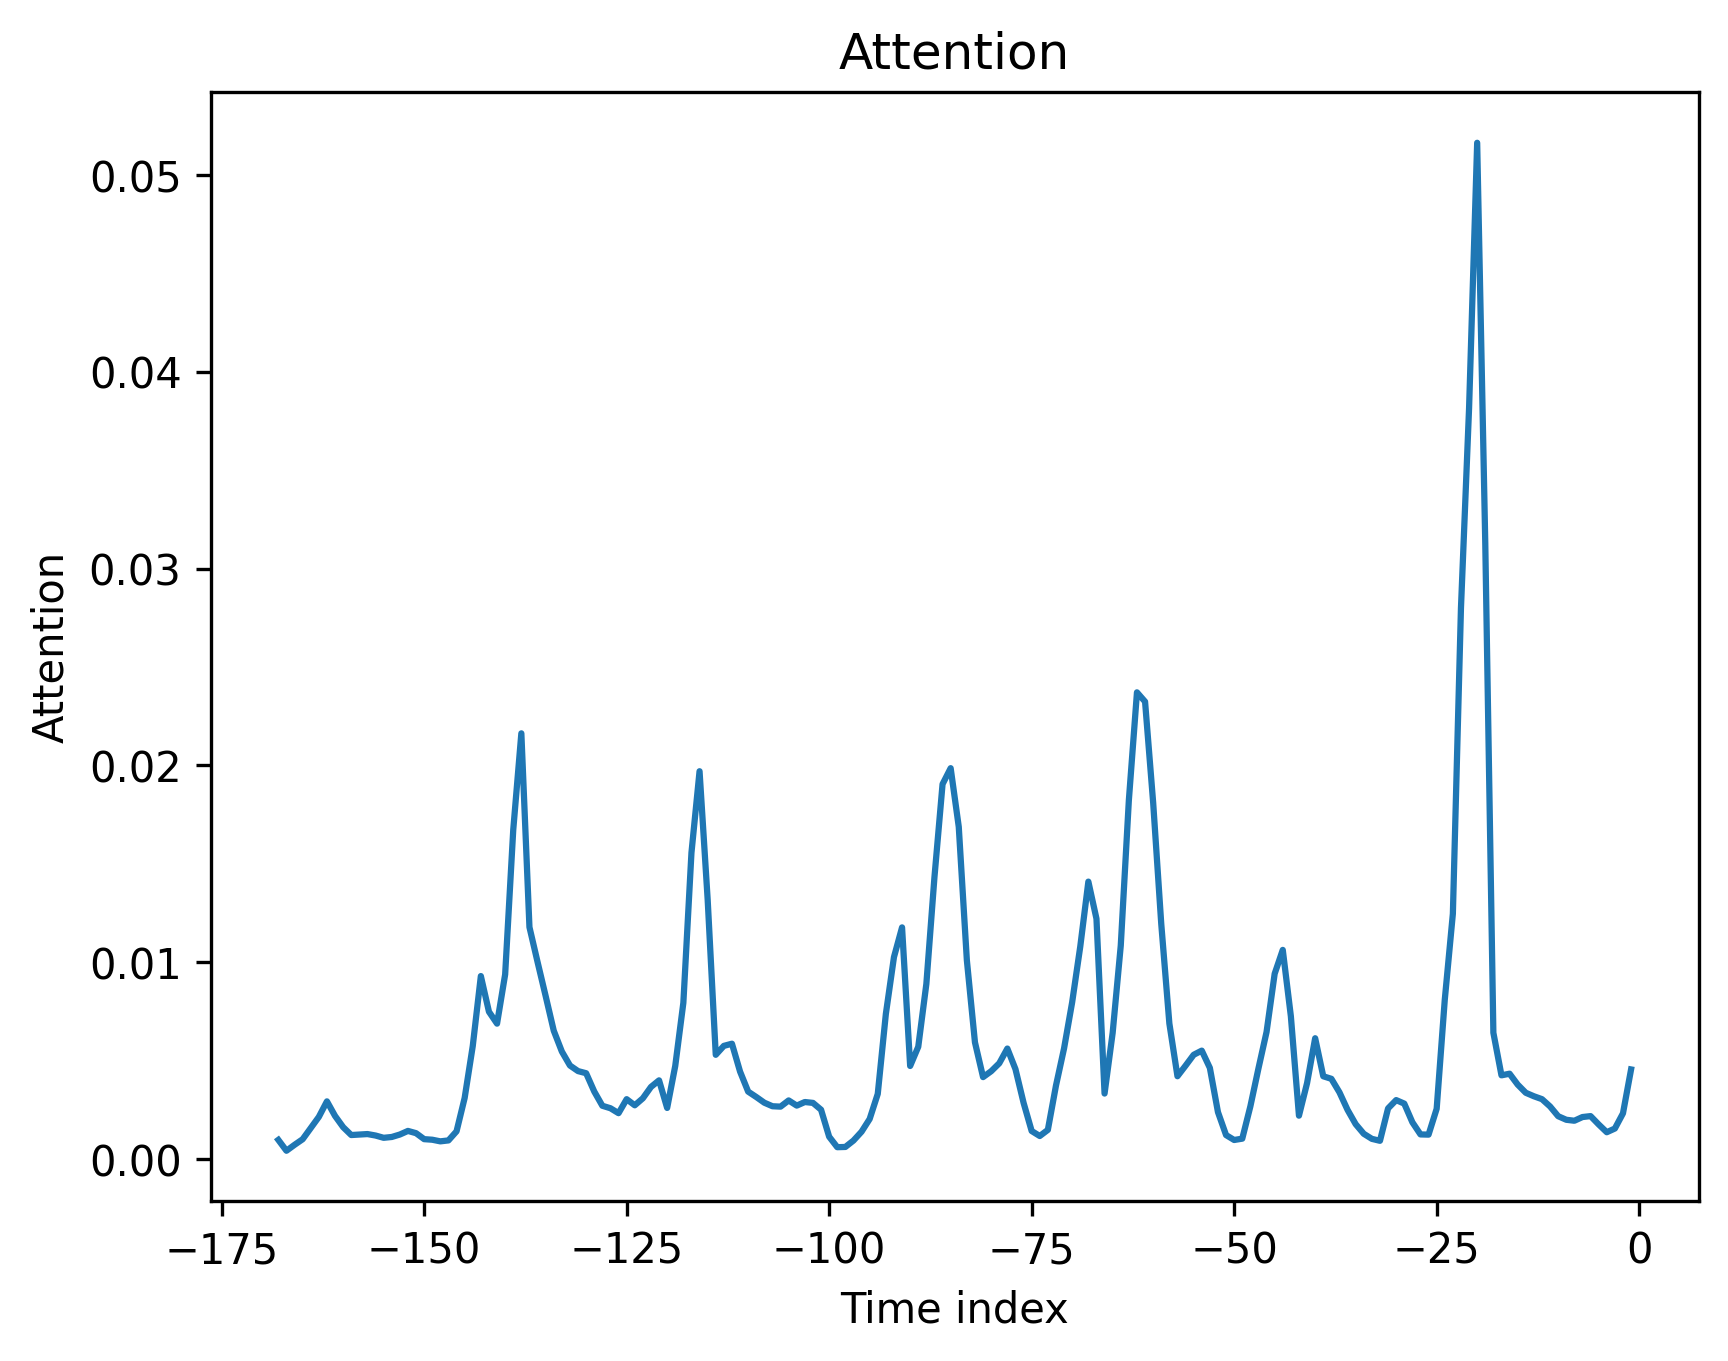
\includegraphics[keepaspectratio]{"./src/attention.pdf"}}
\caption{Focus of the TFT model on temporal patterns}
\end{figure}

    \subsection{Baseline Models
Benchmark}\label{baseline-models-benchmark}

    \paragraph{LSTM Based Models}\label{lstm-based-models}

    At first the dataset which is used by all the upcoming LSTM models is
loaded. After loading, it is split into three intervals: training,
testing, and validation.

    \begin{tcolorbox}[breakable, size=fbox, boxrule=1pt, pad at break*=1mm,colback=cellbackground, colframe=cellborder]
\prompt{In}{incolor}{ }{\boxspacing}
\begin{small}
\begin{Verbatim}[commandchars=\\\{\}]
\PY{n}{X\PYZus{}train}\PY{p}{,} \PY{n}{y\PYZus{}train}\PY{p}{,} \PY{n}{X\PYZus{}test}\PY{p}{,} \PY{n}{y\PYZus{}test}\PY{p}{,} \PY{n}{X\PYZus{}val}\PY{p}{,} \PY{n}{y\PYZus{}val} \PY{o}{=} \PY{n}{train\PYZus{}test\PYZus{}val\PYZus{}split}\PY{p}{(}\PY{n}{lstm\PYZus{}df}\PY{p}{,} \PY{n}{target\PYZus{}column}\PY{o}{=}\PY{l+s+s1}{\PYZsq{}}\PY{l+s+s1}{day\PYZus{}ahead\PYZus{}prices\PYZus{}EURO}\PY{l+s+s1}{\PYZsq{}}\PY{p}{,} 
                                                                      \PY{n}{train\PYZus{}interval}\PY{o}{=}\PY{p}{[}\PY{n}{pd}\PY{o}{.}\PY{n}{Timestamp}\PY{p}{(}\PY{l+s+s1}{\PYZsq{}}\PY{l+s+s1}{2015\PYZhy{}01\PYZhy{}05 00:00:00}\PY{l+s+s1}{\PYZsq{}}\PY{p}{)}\PY{p}{,}
                                                                                      \PY{n}{pd}\PY{o}{.}\PY{n}{Timestamp}\PY{p}{(}\PY{l+s+s1}{\PYZsq{}}\PY{l+s+s1}{2023\PYZhy{}11\PYZhy{}30 23:00:00}\PY{l+s+s1}{\PYZsq{}}\PY{p}{)}\PY{p}{]}\PY{p}{,} 
                                                                      \PY{n}{test\PYZus{}interval}\PY{o}{=}\PY{p}{[}\PY{n}{pd}\PY{o}{.}\PY{n}{Timestamp}\PY{p}{(}\PY{l+s+s1}{\PYZsq{}}\PY{l+s+s1}{2024\PYZhy{}06\PYZhy{}01 00:00:00}\PY{l+s+s1}{\PYZsq{}}\PY{p}{)}\PY{p}{,}
                                                                                     \PY{n}{pd}\PY{o}{.}\PY{n}{Timestamp}\PY{p}{(}\PY{l+s+s1}{\PYZsq{}}\PY{l+s+s1}{2024\PYZhy{}11\PYZhy{}30 23:00:00}\PY{l+s+s1}{\PYZsq{}}\PY{p}{)}\PY{p}{]}\PY{p}{,}
                                                                      \PY{n}{val\PYZus{}interval}\PY{o}{=}\PY{p}{[}\PY{n}{pd}\PY{o}{.}\PY{n}{Timestamp}\PY{p}{(}\PY{l+s+s1}{\PYZsq{}}\PY{l+s+s1}{2023\PYZhy{}12\PYZhy{}01 00:00:00}\PY{l+s+s1}{\PYZsq{}}\PY{p}{)}\PY{p}{,}
                                                                                    \PY{n}{pd}\PY{o}{.}\PY{n}{Timestamp}\PY{p}{(}\PY{l+s+s1}{\PYZsq{}}\PY{l+s+s1}{2024\PYZhy{}05\PYZhy{}31 23:00:00}\PY{l+s+s1}{\PYZsq{}}\PY{p}{)}\PY{p}{]}\PY{p}{)}
\end{Verbatim}
\end{small}
\end{tcolorbox}

    \paragraph{LSTM}\label{lstm}

    An LSTM (Long Short-Term Memory){[}Hochreiter et al.~1997{]} is a type
of RNN (Recurrent Neural Network) designed to address the limitations of
traditional RNNs, particularly in handling long-term dependencies in
sequential data ({[}Bengio et al.~1993{]}, {[}Schmidhuber et
al.~2003{]}). When trying to learn relationships over extended
sequences, LSTMs incorporate mechanisms that allow them to retain
information over long periods. This makes them especially well-suited
for tasks like time series forecasting, where understanding patterns and
dependencies over time is crucial. To also incorporate multiple input
features which might contribute to the day ahead prices, a multivariate
LSTM is used. It takes an input sequence for each input feature and
outputs a fixed length target sequence.

    \begin{tcolorbox}[breakable, size=fbox, boxrule=1pt, pad at break*=1mm,colback=cellbackground, colframe=cellborder]
\prompt{In}{incolor}{ }{\boxspacing}
\begin{small}
\begin{Verbatim}[commandchars=\\\{\}]
\PY{c+c1}{\PYZsh{} define model}
\PY{n}{MultiLSTM} \PY{o}{=} \PY{n}{MultivariateBiLSTM}\PY{p}{(}\PY{n}{features}\PY{o}{=}\PY{n+nb}{list}\PY{p}{(}\PY{n}{X\PYZus{}train}\PY{o}{.}\PY{n}{columns}\PY{p}{)}\PY{p}{,} \PY{n}{target}\PY{o}{=}\PY{l+s+s1}{\PYZsq{}}\PY{l+s+s1}{day\PYZus{}ahead\PYZus{}prices\PYZus{}EURO}\PY{l+s+s1}{\PYZsq{}}\PY{p}{)}
\PY{c+c1}{\PYZsh{} train model}
\PY{n}{training\PYZus{}history} \PY{o}{=} \PY{n}{MultiLSTM}\PY{o}{.}\PY{n}{train}\PY{p}{(}\PY{n}{X\PYZus{}train}\PY{o}{=}\PY{n}{X\PYZus{}train}\PY{p}{,} \PY{n}{y\PYZus{}train}\PY{o}{=}\PY{n}{y\PYZus{}train}\PY{p}{,}
                                \PY{n}{X\PYZus{}val}\PY{o}{=}\PY{n}{X\PYZus{}val}\PY{p}{,} \PY{n}{y\PYZus{}val}\PY{o}{=}\PY{n}{y\PYZus{}val}\PY{p}{,}
                                \PY{n}{X\PYZus{}test}\PY{o}{=}\PY{n}{X\PYZus{}test}\PY{p}{,} \PY{n}{y\PYZus{}test}\PY{o}{=}\PY{n}{y\PYZus{}test}\PY{p}{,}
                                \PY{n}{n\PYZus{}epochs}\PY{o}{=}\PY{l+m+mi}{200}\PY{p}{,} \PY{n}{batch\PYZus{}size}\PY{o}{=}\PY{l+m+mi}{1024}\PY{p}{,} \PY{n}{learning\PYZus{}rate}\PY{o}{=}\PY{l+m+mf}{0.001}\PY{p}{)}
\PY{c+c1}{\PYZsh{} predict}
\PY{n}{prediction\PYZus{}MultiLSTM} \PY{o}{=} \PY{n}{multiLSTM}\PY{o}{.}\PY{n}{run\PYZus{}prediction}\PY{p}{(}\PY{n}{X\PYZus{}test}\PY{p}{)}\PY{o}{.}\PY{n}{set\PYZus{}index}\PY{p}{(}\PY{l+s+s1}{\PYZsq{}}\PY{l+s+s1}{timestamp}\PY{l+s+s1}{\PYZsq{}}\PY{p}{)}
\end{Verbatim}
\end{small}
\end{tcolorbox}

    \subparagraph{Encoder Decoder LSTM}\label{encoder-decoder-lstm}

    Regular multilayer LSTM face several challenges, particularly in tasks
that require a variable length in- or output sequence{[}Hochreiter et
al.~1997{]}. In time series forecasting this is the case when the steps
ahead which need to be predicted differ. Additionally, standard
multilayer LSTM can suffer from information bottlenecks. This is because
the entire input needs to be compressed to a fixed-sized context vector
before generating the output which might lead to information loss
especially for long input sequences{[}Sutskever et al.~2014{]}. Even
though LSTM have the ability to handle the vanishing gradient problem
better than normal RNN, very long sequences can still lead to a
performance decrease ({[}Zhao et al.~2020{]}, {[}Kandadi et
al.~2025{]}).

To address these issues, Seq2Seq (Sequence-to-sequence)
models{[}Sutskever et al.~2014{]} were introduced. These models consist
of two multilayer LSTM's. The first one, the Encoder, processes an
entire sequence of input features at each timestamp. Meaning each block
in the first layer handles one feature. Encoder output and hidden states
are then passes to the second multilayer LSTM, the Decoder. Whose output
is then passed through a linear layer to transform the output dimension
to match the required output sequence length. As a final step and to
ensure the data is in a range between 0 and 1 an sigmoid activation is
applied.

In the below code the Encoder Decoder LSTM is created. For this the
use\_attention is set to False, which applies equal weights to the
encoder output.

    \begin{tcolorbox}[breakable, size=fbox, boxrule=1pt, pad at break*=1mm,colback=cellbackground, colframe=cellborder]
\prompt{In}{incolor}{ }{\boxspacing}
\begin{small}
\begin{Verbatim}[commandchars=\\\{\}]
\PY{c+c1}{\PYZsh{} define model}
\PY{n}{encdecLSTM} \PY{o}{=} \PY{n}{EncoderDecoderAttentionLSTM}\PY{p}{(}\PY{n}{target\PYZus{}length}\PY{o}{=}\PY{l+m+mi}{24}\PY{p}{,} \PY{n}{features}\PY{o}{=}\PY{n+nb}{list}\PY{p}{(}\PY{n}{X\PYZus{}train}\PY{o}{.}\PY{n}{columns}\PY{p}{)}\PY{p}{,} \PY{n}{target}\PY{o}{=}\PY{l+s+s1}{\PYZsq{}}\PY{l+s+s1}{day\PYZus{}ahead\PYZus{}prices\PYZus{}EURO}\PY{l+s+s1}{\PYZsq{}}\PY{p}{,}
                                         \PY{n}{hidden\PYZus{}size}\PY{o}{=}\PY{l+m+mi}{256}\PY{p}{,} \PY{n}{num\PYZus{}layers}\PY{o}{=}\PY{l+m+mi}{6}\PY{p}{,} \PY{n}{use\PYZus{}attention}\PY{o}{=}\PY{k+kc}{False}\PY{p}{)}
\PY{c+c1}{\PYZsh{} train model}
\PY{n}{training\PYZus{}history} \PY{o}{=} \PY{n}{encdecLSTM}\PY{o}{.}\PY{n}{train}\PY{p}{(}\PY{n}{X\PYZus{}train}\PY{o}{=}\PY{n}{X\PYZus{}train}\PY{p}{,} \PY{n}{y\PYZus{}train}\PY{o}{=}\PY{n}{y\PYZus{}train}\PY{p}{,}
                                    \PY{n}{X\PYZus{}val}\PY{o}{=}\PY{n}{X\PYZus{}val}\PY{p}{,} \PY{n}{y\PYZus{}val}\PY{o}{=}\PY{n}{y\PYZus{}val}\PY{p}{,}
                                    \PY{n}{X\PYZus{}test}\PY{o}{=}\PY{n}{X\PYZus{}test}\PY{p}{,} \PY{n}{y\PYZus{}test}\PY{o}{=}\PY{n}{y\PYZus{}test}\PY{p}{,}
                                    \PY{n}{n\PYZus{}epochs}\PY{o}{=}\PY{l+m+mi}{1000}\PY{p}{,} \PY{n}{batch\PYZus{}size}\PY{o}{=}\PY{l+m+mi}{2048}\PY{p}{,} \PY{n}{learning\PYZus{}rate}\PY{o}{=}\PY{l+m+mf}{0.001}\PY{p}{)}
\PY{c+c1}{\PYZsh{} predict}
\PY{n}{prediction\PYZus{}encdecLSTM} \PY{o}{=} \PY{n}{encdecLSTM}\PY{o}{.}\PY{n}{predict}\PY{p}{(}\PY{n}{X}\PY{o}{=}\PY{n}{X\PYZus{}train}\PY{p}{,} \PY{n}{exp\PYZus{}dir}\PY{o}{=}\PY{k+kc}{None}\PY{p}{)}\PY{o}{.}\PY{n}{set\PYZus{}index}\PY{p}{(}\PY{l+s+s1}{\PYZsq{}}\PY{l+s+s1}{timestamp}\PY{l+s+s1}{\PYZsq{}}\PY{p}{)}
\end{Verbatim}
\end{small}
\end{tcolorbox}

    \subparagraph{Incorparate Bahdanau
Attention}\label{incorparate-bahdanau-attention}

    Seq2Seq models without attention face challenges like limited context
representation and difficulty in capturing long-range dependencies.
Instead of relying on a single fixed-length context vector, Bahdanau
attention {[}Bahdanau et al.~2014{]} computes a weighted combination of
input sequence elements for each output time step.

    \begin{figure}
\centering
{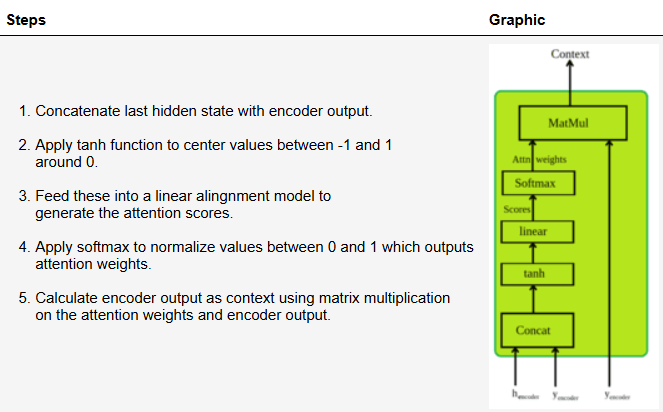
\includegraphics[keepaspectratio]{src/attention_graphic_with_table.png}}
\caption{Attention Mechanism With Table}
\end{figure}

    The above described attention mechanism is used in the Encoder Decoder
Attention LSTM as seen in the green Attention block in the graphic
below.

    \begin{figure}
\centering
{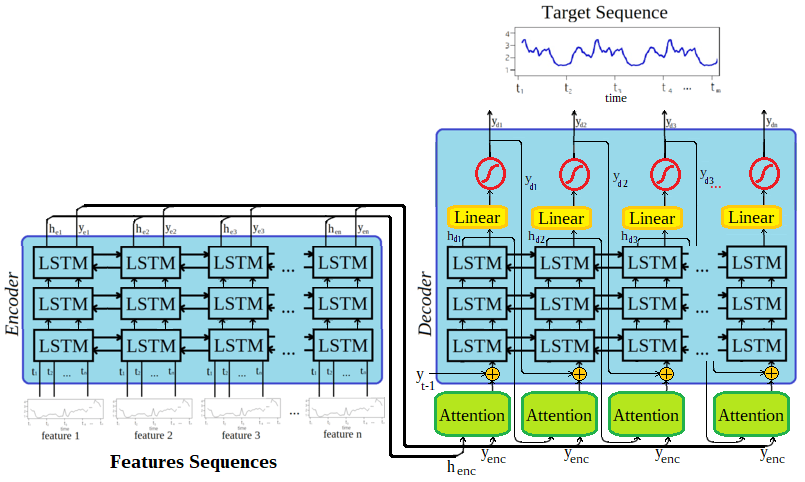
\includegraphics[keepaspectratio]{src/enc_dec_att_LSTM_autoreg.png}}
\caption{Encoder Decoder Attention LSTM}
\end{figure}

    When using the attention mechanism, the context vector is created by
calculating a weighted sum of the encoder's output, while without
attention only the encoder's output is used. This context vector then
gets processed by the decoder to generate the output sequence
step-by-step. Which allows the model to focus on the most relevant parts
of the input sequence when predicting each target value. By leveraging
this mechanism, the model can better handle complex temporal
relationships. This significantly improves performance, especially for
long sequences, as the model does not have to compress all information
into a single bottleneck.

    \begin{tcolorbox}[breakable, size=fbox, boxrule=1pt, pad at break*=1mm,colback=cellbackground, colframe=cellborder]
\prompt{In}{incolor}{ }{\boxspacing}
\begin{small}
\begin{Verbatim}[commandchars=\\\{\}]
\PY{c+c1}{\PYZsh{} define model}
\PY{n}{encdecattLSTM} \PY{o}{=} \PY{n}{EncoderDecoderAttentionLSTM}\PY{p}{(}\PY{n}{target\PYZus{}length}\PY{o}{=}\PY{l+m+mi}{24}\PY{p}{,} \PY{n}{features}\PY{o}{=}\PY{n+nb}{list}\PY{p}{(}\PY{n}{X\PYZus{}train}\PY{o}{.}\PY{n}{columns}\PY{p}{)}\PY{p}{,} \PY{n}{target}\PY{o}{=}\PY{l+s+s1}{\PYZsq{}}\PY{l+s+s1}{day\PYZus{}ahead\PYZus{}prices\PYZus{}EURO}\PY{l+s+s1}{\PYZsq{}}\PY{p}{,}
                                            \PY{n}{hidden\PYZus{}size}\PY{o}{=}\PY{l+m+mi}{256}\PY{p}{,} \PY{n}{num\PYZus{}layers}\PY{o}{=}\PY{l+m+mi}{6}\PY{p}{,} \PY{n}{use\PYZus{}attention}\PY{o}{=}\PY{k+kc}{True}\PY{p}{)}
\PY{c+c1}{\PYZsh{} train model}
\PY{n}{training\PYZus{}history} \PY{o}{=} \PY{n}{encdecattLSTM}\PY{o}{.}\PY{n}{train}\PY{p}{(}\PY{n}{X\PYZus{}train}\PY{o}{=}\PY{n}{X\PYZus{}train}\PY{p}{,} \PY{n}{y\PYZus{}train}\PY{o}{=}\PY{n}{y\PYZus{}train}\PY{p}{,}
                                       \PY{n}{X\PYZus{}val}\PY{o}{=}\PY{n}{X\PYZus{}val}\PY{p}{,} \PY{n}{y\PYZus{}val}\PY{o}{=}\PY{n}{y\PYZus{}val}\PY{p}{,}
                                       \PY{n}{X\PYZus{}test}\PY{o}{=}\PY{n}{X\PYZus{}test}\PY{p}{,} \PY{n}{y\PYZus{}test}\PY{o}{=}\PY{n}{y\PYZus{}test}\PY{p}{,}
                                       \PY{n}{n\PYZus{}epochs}\PY{o}{=}\PY{l+m+mi}{1000}\PY{p}{,} \PY{n}{batch\PYZus{}size}\PY{o}{=}\PY{l+m+mi}{2048}\PY{p}{,} \PY{n}{learning\PYZus{}rate}\PY{o}{=}\PY{l+m+mf}{0.001}\PY{p}{)}
\PY{c+c1}{\PYZsh{} predict}
\PY{n}{prediction\PYZus{}encdecattLSTM} \PY{o}{=} \PY{n}{encdecattLSTM}\PY{o}{.}\PY{n}{predict}\PY{p}{(}\PY{n}{X}\PY{o}{=}\PY{n}{X\PYZus{}train}\PY{p}{,} \PY{n}{exp\PYZus{}dir}\PY{o}{=}\PY{k+kc}{None}\PY{p}{)}\PY{o}{.}\PY{n}{set\PYZus{}index}\PY{p}{(}\PY{l+s+s1}{\PYZsq{}}\PY{l+s+s1}{timestamp}\PY{l+s+s1}{\PYZsq{}}\PY{p}{)}
\end{Verbatim}
\end{small}
\end{tcolorbox}

    \subparagraph{Compare LSTM Models}\label{compare-lstm-models}

    To evaluate which LSTM based model from the above three performs the
best, the MAE is used as metrics.

    \begin{tcolorbox}[breakable, size=fbox, boxrule=1pt, pad at break*=1mm,colback=cellbackground, colframe=cellborder]
\prompt{In}{incolor}{ }{\boxspacing}
\begin{small}
\begin{Verbatim}[commandchars=\\\{\}]
\PY{c+c1}{\PYZsh{} compare LSTM based models on test data}
\PY{n}{BenchMaker} \PY{o}{=} \PY{n}{BenchmarkMaker}\PY{p}{(}\PY{n}{export\PYZus{}dir}\PY{o}{=}\PY{l+s+s1}{\PYZsq{}}\PY{l+s+s1}{result}\PY{l+s+s1}{\PYZsq{}}\PY{p}{)}
\PY{n}{BenchMaker}\PY{o}{.}\PY{n}{load\PYZus{}dataframes}\PY{p}{(}\PY{n}{predictions}\PY{o}{=}\PY{p}{\PYZob{}}\PY{l+s+s1}{\PYZsq{}}\PY{l+s+s1}{MultivarLSTM}\PY{l+s+s1}{\PYZsq{}}\PY{p}{:} \PY{n}{prediction\PYZus{}MultiLSTM}\PY{p}{,}
                                        \PY{l+s+s1}{\PYZsq{}}\PY{l+s+s1}{EncDecAttLSTM}\PY{l+s+s1}{\PYZsq{}}\PY{p}{:} \PY{n}{prediction\PYZus{}encdecLSTM}\PY{p}{,}
                                        \PY{l+s+s1}{\PYZsq{}}\PY{l+s+s1}{EncDecLSTM}\PY{l+s+s1}{\PYZsq{}}\PY{p}{:} \PY{n}{prediction\PYZus{}encdecattLSTM}\PY{p}{\PYZcb{}}\PY{p}{,} \PY{n}{prices}\PY{o}{=}\PY{n}{y\PYZus{}test}\PY{p}{)}
\PY{n}{BenchMaker}\PY{o}{.}\PY{n}{calc\PYZus{}errors}\PY{p}{(}\PY{p}{)}

\PY{n}{BenchMaker}\PY{o}{.}\PY{n}{plot\PYZus{}compare\PYZus{}mae}\PY{p}{(}\PY{p}{)}
\end{Verbatim}
\end{small}
\end{tcolorbox}

    \begin{figure}
\centering
{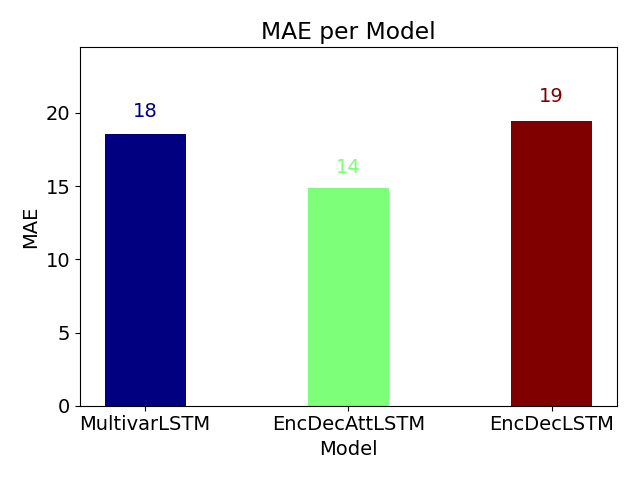
\includegraphics[keepaspectratio, scale = 0.7]{src/compare_LSTM_models_on_val.png}}
\caption{Compare LSTM}
\end{figure}

    As seen in the above graphic is the MAE for the Encoder Decoder
Attention LSTM model much lower than the error of the other two other
LSTM based models. Especially against the Encoder Decoder LSTM without
attention, it shows a much better performance, even though the models
architectures are very similar. This is a good example on how good a
model can get when incorporating an attention mechanism.

    \subsection{Chronos}\label{chronos}

    Chronos is a framework for pre-trained probabilistic time series models
introduced by Ansari et al (2024). As can be seen in the figure below it
tokenizes time series values into a fixed vocabulary through scaling and
quantization and trains transformer-based large language models on these
tokens. Chronos is designed without time-series-specific architecture
except from the tokenization technique, resulting in a minimalist yet
effective approach. Still, the framework achieved remarkable results in
in-domain experiments and demonstrated competitive zero-shot
performance, comparable to models specifically trained on similar tasks.

\begin{figure}
\centering
{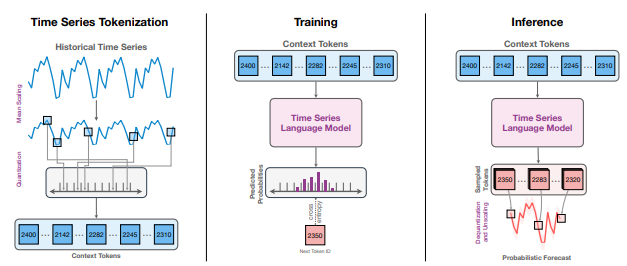
\includegraphics[keepaspectratio]{src/Chronos_Process.png}}
\caption{High-level depiction of Chronos copied from Ansari et al.}
\end{figure}

Chronos is built on Google's T5 architecture, which was introduced by
Vaswani et al.~(2017) and has gained significant popularity since then.
However, a key difference between Chronos and the original T5
architecture is the reduced vocabulary size of 4096 compared to 32128 of
the original T5 architecture, which results in varying parameter counts.
Chronos offers five distinct models, with sizes ranging from 8 million
to 710 million parameters.

    Chronos can further be optimized by fine-tuning it on additional data.
To improve its performance in forecasting the electricity market we used
the day-ahead electricity prices from ENTSO-E as a domain-specific
dataset. The tiny model was chosen for its practicality, as it can be
fine-tuned and utilized for forecasting tasks even on a standard laptop.
To gain deeper insights into the impact of the dataset size and training
steps on model performance, we conducted fine-tuning experiments in four
distinct ways.

As explained in \hyperref[gathering-domain-knowledge]{Section 3} the
day-ahead-prices for energy has experienced heightened volatility in
recent years. To evaluate the impact of dataset characteristics on model
performance, we divided the data into two subsets. The first dataset
contains day-ahead prices from January 2022 to December 2023, and the
second one data spanning from January 2015 to December 2023. The smaller
dataset focuses primarily on recent, highly volatile market conditions,
reflecting current dynamics. In contrast, the larger dataset spans a
longer historical period, capturing a broader range of market scenarios.
This approach enables a direct comparison to determine whether the
smaller, more focused dataset enhances adaptability to recent volatility
or if the larger dataset provides a more comprehensive foundation due to
its diversity. Ansari et al.~propose fine-tuning for 1000 steps and
achieved remarkable results. In a single training step, a batch of
sequences from the dataset is processed to optimize the model's weights.
The input consists of 32 sequences - the batch size and each sequence
contains 512 tokens - the context length. Additionally, to the proposed
1000 training steps we investigated results for 10000 training steps. To
determine which configuration performs best for the challenge of
predicting 24-hour day-ahead energy prices, we conducted hourly
forecasts day by day for an entire year, from the beginning of December
2023 to the end of November 2024. For each forecast day, the context
data consisted of the most recent 512 hourly day-ahead prices.

    The results are computed as following. For each 24 values of one day, we
calculated the root mean squared error and the absolute error. For each
day the mean of these values are calculated and over the whole year the
mean is created again. The results for one year of the Chronos-T5 (Tiny)
model and its fine-tuned versions are presented in the table below.

\rowcolors{2}{white}{gray!25}
{\fontsize{8pt}{10pt}\selectfont\begin{longtable}[]{@{}
  >{\raggedright\arraybackslash}p{(\linewidth - 10\tabcolsep) * \real{0.1667}}
  >{\raggedright\arraybackslash}p{(\linewidth - 10\tabcolsep) * \real{0.1667}}
  >{\raggedright\arraybackslash}p{(\linewidth - 10\tabcolsep) * \real{0.1667}}
  >{\raggedright\arraybackslash}p{(\linewidth - 10\tabcolsep) * \real{0.1667}}
  >{\raggedright\arraybackslash}p{(\linewidth - 10\tabcolsep) * \real{0.1667}}
  >{\raggedright\arraybackslash}p{(\linewidth - 10\tabcolsep) * \real{0.1667}}@{}}
\toprule\noalign{}
\begin{minipage}[b]{\linewidth}\raggedright
Chronos-T5 (Tiny)
\end{minipage} & \begin{minipage}[b]{\linewidth}\raggedright
1. Zero-Shot
\end{minipage} & \begin{minipage}[b]{\linewidth}\raggedright
2. Fine-Tuned Data: 2015 Steps: 1000
\end{minipage} & \begin{minipage}[b]{\linewidth}\raggedright
3. Fine-Tuned Data: 2015 Steps: 10000
\end{minipage} & \begin{minipage}[b]{\linewidth}\raggedright
4. Fine-Tuned Data: 2022 Steps: 1000
\end{minipage} & \begin{minipage}[b]{\linewidth}\raggedright
5. Fine-Tuned Data: 2022 Steps: 10000
\end{minipage} \\
\midrule\noalign{}
\endhead
\bottomrule\noalign{}
\endlastfoot
RMSE & 25.82 & 22.74 & 23.50 & 24.55 & 26.41 \\
MAE & 20.13 & 17.25 & 17.97 & 18.59 & 20.26 \\
\end{longtable}}

    As can be seen in the results not all fine-tuned models outperform the
baseline. Models fine-tuned on the larger dataset, which includes data
from 2015, tend to perform better than those fine-tuned on the smaller,
more recent dataset. This may be due to the fact that, although the
energy market is currently highly volatile, less volatile days dominate
the market, making the larger dataset, with its broader range of
scenarios, more beneficial. Furthermore, models trained with 1,000 steps
tend to outperform those trained with 10,000 steps, likely because the
latter suffer from overfitting.

We initially aimed to analyze the MAE percentage and RMSE percentage
values. However, because the actual day-ahead price is close to zero on
some days, these metrics become extremely high and less reliable.
Therefore, we focus on the RMSE and MAE absolute values for a more
reliable evaluation.

The model which was fine-tuned on the large dataset with 1000 training
steps performs the best. This model has the lowest RMSE and MAE. On
average the difference between the predicted hourly day-ahead price and
its actual value is 17.254 Euros.

Model five is outperformed by the baseline in all metrics.

    We use both the uploaded fine-tuned models and a pretrained model to
forecast a defined period. A comparison of Model One and Model Two is
visualized in the following two graphs. Each model forecasts the period
from February 14, 2024, to February 23, 2024, which includes the
challenge date---February 18---exactly one year earlier.

    \begin{tcolorbox}[breakable, size=fbox, boxrule=1pt, pad at break*=1mm,colback=cellbackground, colframe=cellborder]
\prompt{In}{incolor}{5}{\boxspacing}
\begin{small}
\begin{Verbatim}[commandchars=\\\{\}]
\PY{n}{start\PYZus{}time} \PY{o}{=} \PY{l+s+s2}{\PYZdq{}}\PY{l+s+s2}{2024\PYZhy{}02\PYZhy{}14 00:00:00}\PY{l+s+s2}{\PYZdq{}}
\PY{n}{end\PYZus{}time} \PY{o}{=} \PY{l+s+s2}{\PYZdq{}}\PY{l+s+s2}{2024\PYZhy{}02\PYZhy{}22 23:00:00}\PY{l+s+s2}{\PYZdq{}}

\PY{n}{model1} \PY{o}{=} \PY{l+s+s2}{\PYZdq{}}\PY{l+s+s2}{amazon/chronos\PYZhy{}t5\PYZhy{}tiny}\PY{l+s+s2}{\PYZdq{}}
\PY{n}{forecast1} \PY{o}{=} \PY{n}{chronosForecast}\PY{p}{(}\PY{n}{model1}\PY{p}{,} \PY{n}{start\PYZus{}time}\PY{p}{,} \PY{n}{end\PYZus{}time}\PY{p}{)}

\PY{n}{model2} \PY{o}{=} \PY{l+s+s2}{\PYZdq{}}\PY{l+s+s2}{juliushanusch/chronos\PYZhy{}tiny\PYZhy{}fine\PYZhy{}tuned\PYZhy{}day\PYZhy{}ahead\PYZhy{}prices}\PY{l+s+s2}{\PYZdq{}}
\PY{n}{forecast2} \PY{o}{=} \PY{n}{chronosForecast}\PY{p}{(}\PY{n}{model2}\PY{p}{,} \PY{n}{start\PYZus{}time}\PY{p}{,} \PY{n}{end\PYZus{}time}\PY{p}{)}
\end{Verbatim}
\end{small}
\end{tcolorbox}

    \begin{tcolorbox}[breakable, size=fbox, boxrule=1pt, pad at break*=1mm,colback=cellbackground, colframe=cellborder]
\prompt{In}{incolor}{8}{\boxspacing}
\begin{small}
\begin{Verbatim}[commandchars=\\\{\}]
\PY{c+c1}{\PYZsh{} Set up the figure with two subplots (1 row, 2 columns)}
\PY{n}{fig}\PY{p}{,} \PY{n}{axs} \PY{o}{=} \PY{n}{plt}\PY{o}{.}\PY{n}{subplots}\PY{p}{(}\PY{l+m+mi}{1}\PY{p}{,} \PY{l+m+mi}{2}\PY{p}{,} \PY{n}{figsize}\PY{o}{=}\PY{p}{(}\PY{l+m+mi}{15}\PY{p}{,} \PY{l+m+mi}{6}\PY{p}{)}\PY{p}{)}

\PY{c+c1}{\PYZsh{} Plot for model1 (forecast1)}
\PY{n}{axs}\PY{p}{[}\PY{l+m+mi}{0}\PY{p}{]}\PY{o}{.}\PY{n}{plot}\PY{p}{(}\PY{n}{forecast1}\PY{p}{[}\PY{l+s+s1}{\PYZsq{}}\PY{l+s+s1}{timestamp}\PY{l+s+s1}{\PYZsq{}}\PY{p}{]}\PY{p}{,} \PY{n}{forecast1}\PY{p}{[}\PY{l+s+s1}{\PYZsq{}}\PY{l+s+s1}{actual\PYZus{}value}\PY{l+s+s1}{\PYZsq{}}\PY{p}{]}\PY{p}{,} \PY{n}{label}\PY{o}{=}\PY{l+s+s1}{\PYZsq{}}\PY{l+s+s1}{Actual}\PY{l+s+s1}{\PYZsq{}}\PY{p}{,} \PY{n}{color}\PY{o}{=}\PY{l+s+s1}{\PYZsq{}}\PY{l+s+s1}{blue}\PY{l+s+s1}{\PYZsq{}}\PY{p}{,} \PY{n}{linestyle}\PY{o}{=}\PY{l+s+s1}{\PYZsq{}}\PY{l+s+s1}{\PYZhy{}}\PY{l+s+s1}{\PYZsq{}}\PY{p}{,} \PY{n}{linewidth}\PY{o}{=}\PY{l+m+mi}{2}\PY{p}{)}
\PY{n}{axs}\PY{p}{[}\PY{l+m+mi}{0}\PY{p}{]}\PY{o}{.}\PY{n}{plot}\PY{p}{(}\PY{n}{forecast1}\PY{p}{[}\PY{l+s+s1}{\PYZsq{}}\PY{l+s+s1}{timestamp}\PY{l+s+s1}{\PYZsq{}}\PY{p}{]}\PY{p}{,} \PY{n}{forecast1}\PY{p}{[}\PY{l+s+s1}{\PYZsq{}}\PY{l+s+s1}{forecasted\PYZus{}values}\PY{l+s+s1}{\PYZsq{}}\PY{p}{]}\PY{p}{,} \PY{n}{label}\PY{o}{=}\PY{l+s+s1}{\PYZsq{}}\PY{l+s+s1}{Forecasted}\PY{l+s+s1}{\PYZsq{}}\PY{p}{,} \PY{n}{color}\PY{o}{=}\PY{l+s+s1}{\PYZsq{}}\PY{l+s+s1}{orange}\PY{l+s+s1}{\PYZsq{}}\PY{p}{,} \PY{n}{linestyle}\PY{o}{=}\PY{l+s+s1}{\PYZsq{}}\PY{l+s+s1}{\PYZhy{}\PYZhy{}}\PY{l+s+s1}{\PYZsq{}}\PY{p}{,} \PY{n}{linewidth}\PY{o}{=}\PY{l+m+mi}{2}\PY{p}{)}
\PY{n}{axs}\PY{p}{[}\PY{l+m+mi}{0}\PY{p}{]}\PY{o}{.}\PY{n}{plot}\PY{p}{(}\PY{n}{forecast1}\PY{p}{[}\PY{l+s+s1}{\PYZsq{}}\PY{l+s+s1}{timestamp}\PY{l+s+s1}{\PYZsq{}}\PY{p}{]}\PY{p}{,} \PY{n}{forecast1}\PY{p}{[}\PY{l+s+s1}{\PYZsq{}}\PY{l+s+s1}{absolute\PYZus{}error}\PY{l+s+s1}{\PYZsq{}}\PY{p}{]}\PY{p}{,} \PY{n}{label}\PY{o}{=}\PY{l+s+s1}{\PYZsq{}}\PY{l+s+s1}{Absolute Error}\PY{l+s+s1}{\PYZsq{}}\PY{p}{,} \PY{n}{color}\PY{o}{=}\PY{l+s+s1}{\PYZsq{}}\PY{l+s+s1}{red}\PY{l+s+s1}{\PYZsq{}}\PY{p}{,} \PY{n}{linestyle}\PY{o}{=}\PY{l+s+s1}{\PYZsq{}}\PY{l+s+s1}{:}\PY{l+s+s1}{\PYZsq{}}\PY{p}{,} \PY{n}{linewidth}\PY{o}{=}\PY{l+m+mi}{2}\PY{p}{)}

\PY{n}{axs}\PY{p}{[}\PY{l+m+mi}{0}\PY{p}{]}\PY{o}{.}\PY{n}{set\PYZus{}xlabel}\PY{p}{(}\PY{l+s+s1}{\PYZsq{}}\PY{l+s+s1}{Timestamp}\PY{l+s+s1}{\PYZsq{}}\PY{p}{)}
\PY{n}{axs}\PY{p}{[}\PY{l+m+mi}{0}\PY{p}{]}\PY{o}{.}\PY{n}{set\PYZus{}ylabel}\PY{p}{(}\PY{l+s+s1}{\PYZsq{}}\PY{l+s+s1}{Value}\PY{l+s+s1}{\PYZsq{}}\PY{p}{)}
\PY{n}{axs}\PY{p}{[}\PY{l+m+mi}{0}\PY{p}{]}\PY{o}{.}\PY{n}{set\PYZus{}title}\PY{p}{(}\PY{l+s+sa}{f}\PY{l+s+s1}{\PYZsq{}}\PY{l+s+s1}{Actual vs Forecasted Values with Absolute Error }\PY{l+s+se}{\PYZbs{}n}\PY{l+s+s1}{ Model: }\PY{l+s+si}{\PYZob{}}\PY{n}{model1}\PY{l+s+si}{\PYZcb{}}\PY{l+s+s1}{\PYZsq{}}\PY{p}{)}
\PY{n}{axs}\PY{p}{[}\PY{l+m+mi}{0}\PY{p}{]}\PY{o}{.}\PY{n}{legend}\PY{p}{(}\PY{p}{)}
\PY{n}{axs}\PY{p}{[}\PY{l+m+mi}{0}\PY{p}{]}\PY{o}{.}\PY{n}{tick\PYZus{}params}\PY{p}{(}\PY{n}{axis}\PY{o}{=}\PY{l+s+s1}{\PYZsq{}}\PY{l+s+s1}{x}\PY{l+s+s1}{\PYZsq{}}\PY{p}{,} \PY{n}{rotation}\PY{o}{=}\PY{l+m+mi}{45}\PY{p}{)}

\PY{c+c1}{\PYZsh{} Plot for model2 (forecast2)}
\PY{n}{axs}\PY{p}{[}\PY{l+m+mi}{1}\PY{p}{]}\PY{o}{.}\PY{n}{plot}\PY{p}{(}\PY{n}{forecast2}\PY{p}{[}\PY{l+s+s1}{\PYZsq{}}\PY{l+s+s1}{timestamp}\PY{l+s+s1}{\PYZsq{}}\PY{p}{]}\PY{p}{,} \PY{n}{forecast2}\PY{p}{[}\PY{l+s+s1}{\PYZsq{}}\PY{l+s+s1}{actual\PYZus{}value}\PY{l+s+s1}{\PYZsq{}}\PY{p}{]}\PY{p}{,} \PY{n}{label}\PY{o}{=}\PY{l+s+s1}{\PYZsq{}}\PY{l+s+s1}{Actual}\PY{l+s+s1}{\PYZsq{}}\PY{p}{,} \PY{n}{color}\PY{o}{=}\PY{l+s+s1}{\PYZsq{}}\PY{l+s+s1}{blue}\PY{l+s+s1}{\PYZsq{}}\PY{p}{,} \PY{n}{linestyle}\PY{o}{=}\PY{l+s+s1}{\PYZsq{}}\PY{l+s+s1}{\PYZhy{}}\PY{l+s+s1}{\PYZsq{}}\PY{p}{,} \PY{n}{linewidth}\PY{o}{=}\PY{l+m+mi}{2}\PY{p}{)}
\PY{n}{axs}\PY{p}{[}\PY{l+m+mi}{1}\PY{p}{]}\PY{o}{.}\PY{n}{plot}\PY{p}{(}\PY{n}{forecast2}\PY{p}{[}\PY{l+s+s1}{\PYZsq{}}\PY{l+s+s1}{timestamp}\PY{l+s+s1}{\PYZsq{}}\PY{p}{]}\PY{p}{,} \PY{n}{forecast2}\PY{p}{[}\PY{l+s+s1}{\PYZsq{}}\PY{l+s+s1}{forecasted\PYZus{}values}\PY{l+s+s1}{\PYZsq{}}\PY{p}{]}\PY{p}{,} \PY{n}{label}\PY{o}{=}\PY{l+s+s1}{\PYZsq{}}\PY{l+s+s1}{Forecasted}\PY{l+s+s1}{\PYZsq{}}\PY{p}{,} \PY{n}{color}\PY{o}{=}\PY{l+s+s1}{\PYZsq{}}\PY{l+s+s1}{orange}\PY{l+s+s1}{\PYZsq{}}\PY{p}{,} \PY{n}{linestyle}\PY{o}{=}\PY{l+s+s1}{\PYZsq{}}\PY{l+s+s1}{\PYZhy{}\PYZhy{}}\PY{l+s+s1}{\PYZsq{}}\PY{p}{,} \PY{n}{linewidth}\PY{o}{=}\PY{l+m+mi}{2}\PY{p}{)}
\PY{n}{axs}\PY{p}{[}\PY{l+m+mi}{1}\PY{p}{]}\PY{o}{.}\PY{n}{plot}\PY{p}{(}\PY{n}{forecast2}\PY{p}{[}\PY{l+s+s1}{\PYZsq{}}\PY{l+s+s1}{timestamp}\PY{l+s+s1}{\PYZsq{}}\PY{p}{]}\PY{p}{,} \PY{n}{forecast2}\PY{p}{[}\PY{l+s+s1}{\PYZsq{}}\PY{l+s+s1}{absolute\PYZus{}error}\PY{l+s+s1}{\PYZsq{}}\PY{p}{]}\PY{p}{,} \PY{n}{label}\PY{o}{=}\PY{l+s+s1}{\PYZsq{}}\PY{l+s+s1}{Absolute Error}\PY{l+s+s1}{\PYZsq{}}\PY{p}{,} \PY{n}{color}\PY{o}{=}\PY{l+s+s1}{\PYZsq{}}\PY{l+s+s1}{red}\PY{l+s+s1}{\PYZsq{}}\PY{p}{,} \PY{n}{linestyle}\PY{o}{=}\PY{l+s+s1}{\PYZsq{}}\PY{l+s+s1}{:}\PY{l+s+s1}{\PYZsq{}}\PY{p}{,} \PY{n}{linewidth}\PY{o}{=}\PY{l+m+mi}{2}\PY{p}{)}

\PY{n}{axs}\PY{p}{[}\PY{l+m+mi}{1}\PY{p}{]}\PY{o}{.}\PY{n}{set\PYZus{}xlabel}\PY{p}{(}\PY{l+s+s1}{\PYZsq{}}\PY{l+s+s1}{Timestamp}\PY{l+s+s1}{\PYZsq{}}\PY{p}{)}
\PY{n}{axs}\PY{p}{[}\PY{l+m+mi}{1}\PY{p}{]}\PY{o}{.}\PY{n}{set\PYZus{}ylabel}\PY{p}{(}\PY{l+s+s1}{\PYZsq{}}\PY{l+s+s1}{Value}\PY{l+s+s1}{\PYZsq{}}\PY{p}{)}
\PY{n}{axs}\PY{p}{[}\PY{l+m+mi}{1}\PY{p}{]}\PY{o}{.}\PY{n}{set\PYZus{}title}\PY{p}{(}\PY{l+s+sa}{f}\PY{l+s+s1}{\PYZsq{}}\PY{l+s+s1}{Actual vs Forecasted Values with Absolute Error }\PY{l+s+se}{\PYZbs{}n}\PY{l+s+s1}{ Model: }\PY{l+s+si}{\PYZob{}}\PY{n}{model2}\PY{l+s+si}{\PYZcb{}}\PY{l+s+s1}{\PYZsq{}}\PY{p}{)}
\PY{n}{axs}\PY{p}{[}\PY{l+m+mi}{1}\PY{p}{]}\PY{o}{.}\PY{n}{legend}\PY{p}{(}\PY{p}{)}
\PY{n}{axs}\PY{p}{[}\PY{l+m+mi}{1}\PY{p}{]}\PY{o}{.}\PY{n}{tick\PYZus{}params}\PY{p}{(}\PY{n}{axis}\PY{o}{=}\PY{l+s+s1}{\PYZsq{}}\PY{l+s+s1}{x}\PY{l+s+s1}{\PYZsq{}}\PY{p}{,} \PY{n}{rotation}\PY{o}{=}\PY{l+m+mi}{45}\PY{p}{)}

\PY{n}{axs}\PY{p}{[}\PY{l+m+mi}{0}\PY{p}{]}\PY{o}{.}\PY{n}{grid}\PY{p}{(}\PY{k+kc}{True}\PY{p}{,} \PY{n}{linewidth}\PY{o}{=}\PY{l+m+mf}{0.5}\PY{p}{,} \PY{n}{linestyle}\PY{o}{=}\PY{l+s+s1}{\PYZsq{}}\PY{l+s+s1}{\PYZhy{}\PYZhy{}}\PY{l+s+s1}{\PYZsq{}}\PY{p}{,} \PY{n}{alpha}\PY{o}{=}\PY{l+m+mf}{0.7}\PY{p}{)}
\PY{n}{axs}\PY{p}{[}\PY{l+m+mi}{1}\PY{p}{]}\PY{o}{.}\PY{n}{grid}\PY{p}{(}\PY{k+kc}{True}\PY{p}{,} \PY{n}{linewidth}\PY{o}{=}\PY{l+m+mf}{0.5}\PY{p}{,} \PY{n}{linestyle}\PY{o}{=}\PY{l+s+s1}{\PYZsq{}}\PY{l+s+s1}{\PYZhy{}\PYZhy{}}\PY{l+s+s1}{\PYZsq{}}\PY{p}{,} \PY{n}{alpha}\PY{o}{=}\PY{l+m+mf}{0.7}\PY{p}{)}


\PY{c+c1}{\PYZsh{} Adjust the layout to make sure there is no overlap}
\PY{n}{plt}\PY{o}{.}\PY{n}{tight\PYZus{}layout}\PY{p}{(}\PY{p}{)}

\PY{c+c1}{\PYZsh{} Show the plot}
\PY{n}{plt}\PY{o}{.}\PY{n}{show}\PY{p}{(}\PY{p}{)}
\end{Verbatim}
\end{small}
\end{tcolorbox}

    \begin{center}
    \adjustimage{max size={0.9\linewidth}{0.9\paperheight}}{output_119_0.png}
    \end{center}
    { \hspace*{\fill} \\}
    
    As previously mentioned, several sizes of Chronos models are available.
In addition to the Chronos-T5 (Tiny) model, we evaluated the performance
of the Chronos-T5 (Large) model. For this model, we applied the same
fine-tuning steps as we did for the Chronos-T5 (Tiny) model. The
Chronos-T5 (Large) model contains approximately 88 times more parameters
compared to the tiny model and is therefore expected to perform better
than the Chronos-T5 (Tiny) model. However, this comes at the cost of
significantly higher computational requirements, both in terms of
training and forecasting.

    The yearly Results of the Chronos-T5 (Large) model and its fine-tuned
versions are presented in the table below.

\rowcolors{2}{white}{gray!25}
{\fontsize{8pt}{10pt}\selectfont\begin{longtable}[]{@{}
  >{\raggedright\arraybackslash}p{(\linewidth - 10\tabcolsep) * \real{0.1667}}
  >{\raggedright\arraybackslash}p{(\linewidth - 10\tabcolsep) * \real{0.1667}}
  >{\raggedright\arraybackslash}p{(\linewidth - 10\tabcolsep) * \real{0.1667}}
  >{\raggedright\arraybackslash}p{(\linewidth - 10\tabcolsep) * \real{0.1667}}
  >{\raggedright\arraybackslash}p{(\linewidth - 10\tabcolsep) * \real{0.1667}}
  >{\raggedright\arraybackslash}p{(\linewidth - 10\tabcolsep) * \real{0.1667}}@{}}
\toprule\noalign{}
\begin{minipage}[b]{\linewidth}\raggedright
Chronos-T5 (Large)
\end{minipage} & \begin{minipage}[b]{\linewidth}\raggedright
1. Zero-Shot
\end{minipage} & \begin{minipage}[b]{\linewidth}\raggedright
2. Fine-Tuned Data: 2015 Steps: 1000
\end{minipage} & \begin{minipage}[b]{\linewidth}\raggedright
3. Fine-Tuned Data: 2015 Steps: 10000
\end{minipage} & \begin{minipage}[b]{\linewidth}\raggedright
4. Fine-Tuned Data: 2022 Steps: 1000
\end{minipage} & \begin{minipage}[b]{\linewidth}\raggedright
5. Fine-Tuned Data: 2022 Steps: 10000
\end{minipage} \\
\midrule\noalign{}
\endhead
\bottomrule\noalign{}
\endlastfoot
RMSE & 22.45 & 21.05 & 22.07 & 22.74 & 22.30 \\
MAE & 17.14 & 15.85 & 16.75 & 17.18 & 16.95 \\
\end{longtable}}

    As expected, the large model performs better compared to the tiny
models. We observe similar results in fine-tuning as seen with the tiny
models. Once again, the models trained on the smaller dataset outperform
those trained on the larger dataset. Interestingly, the non-fine-tuned
Chronos-T5 (Large) model performs quite similarly to the Chronos-T5
(Tiny) model fine-tuned on the larger dataset with 1,000 training steps.

Model two emerges as the best-performing model overall. It achieves an
average difference of just 15.85 Euros.

    The comparison of the large fine-tuned model number two with model
number one is visualized in the graphs below.

    \begin{tcolorbox}[breakable, size=fbox, boxrule=1pt, pad at break*=1mm,colback=cellbackground, colframe=cellborder]
\prompt{In}{incolor}{9}{\boxspacing}
\begin{small}
\begin{Verbatim}[commandchars=\\\{\}]
\PY{n}{model3} \PY{o}{=} \PY{l+s+s2}{\PYZdq{}}\PY{l+s+s2}{amazon/chronos\PYZhy{}t5\PYZhy{}large}\PY{l+s+s2}{\PYZdq{}}
\PY{n}{forecast3} \PY{o}{=} \PY{n}{chronosForecast}\PY{p}{(}\PY{n}{model1}\PY{p}{,} \PY{n}{start\PYZus{}time}\PY{p}{,} \PY{n}{end\PYZus{}time}\PY{p}{)}

\PY{n}{model4} \PY{o}{=} \PY{l+s+s2}{\PYZdq{}}\PY{l+s+s2}{juliushanusch/chronos\PYZhy{}large\PYZhy{}fine\PYZhy{}tuned\PYZhy{}day\PYZhy{}ahead\PYZhy{}prices}\PY{l+s+s2}{\PYZdq{}}
\PY{n}{forecast4} \PY{o}{=} \PY{n}{chronosForecast}\PY{p}{(}\PY{n}{model2}\PY{p}{,} \PY{n}{start\PYZus{}time}\PY{p}{,} \PY{n}{end\PYZus{}time}\PY{p}{)}
\end{Verbatim}
\end{small}
\end{tcolorbox}

    \begin{tcolorbox}[breakable, size=fbox, boxrule=1pt, pad at break*=1mm,colback=cellbackground, colframe=cellborder]
\prompt{In}{incolor}{10}{\boxspacing}
\begin{small}
\begin{Verbatim}[commandchars=\\\{\}]
    

\PY{c+c1}{\PYZsh{} Set up the figure with two subplots (1 row, 2 columns)}
\PY{n}{fig}\PY{p}{,} \PY{n}{axs} \PY{o}{=} \PY{n}{plt}\PY{o}{.}\PY{n}{subplots}\PY{p}{(}\PY{l+m+mi}{1}\PY{p}{,} \PY{l+m+mi}{2}\PY{p}{,} \PY{n}{figsize}\PY{o}{=}\PY{p}{(}\PY{l+m+mi}{15}\PY{p}{,} \PY{l+m+mi}{6}\PY{p}{)}\PY{p}{)}

\PY{c+c1}{\PYZsh{} Plot for model1 (forecast1)}
\PY{n}{axs}\PY{p}{[}\PY{l+m+mi}{0}\PY{p}{]}\PY{o}{.}\PY{n}{plot}\PY{p}{(}\PY{n}{forecast3}\PY{p}{[}\PY{l+s+s1}{\PYZsq{}}\PY{l+s+s1}{timestamp}\PY{l+s+s1}{\PYZsq{}}\PY{p}{]}\PY{p}{,} \PY{n}{forecast3}\PY{p}{[}\PY{l+s+s1}{\PYZsq{}}\PY{l+s+s1}{actual\PYZus{}value}\PY{l+s+s1}{\PYZsq{}}\PY{p}{]}\PY{p}{,} \PY{n}{label}\PY{o}{=}\PY{l+s+s1}{\PYZsq{}}\PY{l+s+s1}{Actual}\PY{l+s+s1}{\PYZsq{}}\PY{p}{,} \PY{n}{color}\PY{o}{=}\PY{l+s+s1}{\PYZsq{}}\PY{l+s+s1}{blue}\PY{l+s+s1}{\PYZsq{}}\PY{p}{,} \PY{n}{linestyle}\PY{o}{=}\PY{l+s+s1}{\PYZsq{}}\PY{l+s+s1}{\PYZhy{}}\PY{l+s+s1}{\PYZsq{}}\PY{p}{,} \PY{n}{linewidth}\PY{o}{=}\PY{l+m+mi}{2}\PY{p}{)}
\PY{n}{axs}\PY{p}{[}\PY{l+m+mi}{0}\PY{p}{]}\PY{o}{.}\PY{n}{plot}\PY{p}{(}\PY{n}{forecast3}\PY{p}{[}\PY{l+s+s1}{\PYZsq{}}\PY{l+s+s1}{timestamp}\PY{l+s+s1}{\PYZsq{}}\PY{p}{]}\PY{p}{,} \PY{n}{forecast3}\PY{p}{[}\PY{l+s+s1}{\PYZsq{}}\PY{l+s+s1}{forecasted\PYZus{}values}\PY{l+s+s1}{\PYZsq{}}\PY{p}{]}\PY{p}{,} \PY{n}{label}\PY{o}{=}\PY{l+s+s1}{\PYZsq{}}\PY{l+s+s1}{Forecasted}\PY{l+s+s1}{\PYZsq{}}\PY{p}{,} \PY{n}{color}\PY{o}{=}\PY{l+s+s1}{\PYZsq{}}\PY{l+s+s1}{orange}\PY{l+s+s1}{\PYZsq{}}\PY{p}{,} \PY{n}{linestyle}\PY{o}{=}\PY{l+s+s1}{\PYZsq{}}\PY{l+s+s1}{\PYZhy{}\PYZhy{}}\PY{l+s+s1}{\PYZsq{}}\PY{p}{,} \PY{n}{linewidth}\PY{o}{=}\PY{l+m+mi}{2}\PY{p}{)}
\PY{n}{axs}\PY{p}{[}\PY{l+m+mi}{0}\PY{p}{]}\PY{o}{.}\PY{n}{plot}\PY{p}{(}\PY{n}{forecast3}\PY{p}{[}\PY{l+s+s1}{\PYZsq{}}\PY{l+s+s1}{timestamp}\PY{l+s+s1}{\PYZsq{}}\PY{p}{]}\PY{p}{,} \PY{n}{forecast3}\PY{p}{[}\PY{l+s+s1}{\PYZsq{}}\PY{l+s+s1}{absolute\PYZus{}error}\PY{l+s+s1}{\PYZsq{}}\PY{p}{]}\PY{p}{,} \PY{n}{label}\PY{o}{=}\PY{l+s+s1}{\PYZsq{}}\PY{l+s+s1}{Absolute Error}\PY{l+s+s1}{\PYZsq{}}\PY{p}{,} \PY{n}{color}\PY{o}{=}\PY{l+s+s1}{\PYZsq{}}\PY{l+s+s1}{red}\PY{l+s+s1}{\PYZsq{}}\PY{p}{,} \PY{n}{linestyle}\PY{o}{=}\PY{l+s+s1}{\PYZsq{}}\PY{l+s+s1}{:}\PY{l+s+s1}{\PYZsq{}}\PY{p}{,} \PY{n}{linewidth}\PY{o}{=}\PY{l+m+mi}{2}\PY{p}{)}

\PY{n}{axs}\PY{p}{[}\PY{l+m+mi}{0}\PY{p}{]}\PY{o}{.}\PY{n}{set\PYZus{}xlabel}\PY{p}{(}\PY{l+s+s1}{\PYZsq{}}\PY{l+s+s1}{Timestamp}\PY{l+s+s1}{\PYZsq{}}\PY{p}{)}
\PY{n}{axs}\PY{p}{[}\PY{l+m+mi}{0}\PY{p}{]}\PY{o}{.}\PY{n}{set\PYZus{}ylabel}\PY{p}{(}\PY{l+s+s1}{\PYZsq{}}\PY{l+s+s1}{Value}\PY{l+s+s1}{\PYZsq{}}\PY{p}{)}
\PY{n}{axs}\PY{p}{[}\PY{l+m+mi}{0}\PY{p}{]}\PY{o}{.}\PY{n}{set\PYZus{}title}\PY{p}{(}\PY{l+s+sa}{f}\PY{l+s+s1}{\PYZsq{}}\PY{l+s+s1}{Actual vs Forecasted Values with Absolute Error }\PY{l+s+se}{\PYZbs{}n}\PY{l+s+s1}{ Model: }\PY{l+s+si}{\PYZob{}}\PY{n}{model3}\PY{l+s+si}{\PYZcb{}}\PY{l+s+s1}{\PYZsq{}}\PY{p}{)}
\PY{n}{axs}\PY{p}{[}\PY{l+m+mi}{0}\PY{p}{]}\PY{o}{.}\PY{n}{legend}\PY{p}{(}\PY{p}{)}
\PY{n}{axs}\PY{p}{[}\PY{l+m+mi}{0}\PY{p}{]}\PY{o}{.}\PY{n}{tick\PYZus{}params}\PY{p}{(}\PY{n}{axis}\PY{o}{=}\PY{l+s+s1}{\PYZsq{}}\PY{l+s+s1}{x}\PY{l+s+s1}{\PYZsq{}}\PY{p}{,} \PY{n}{rotation}\PY{o}{=}\PY{l+m+mi}{45}\PY{p}{)}

\PY{c+c1}{\PYZsh{} Plot for model2 (forecast2)}
\PY{n}{axs}\PY{p}{[}\PY{l+m+mi}{1}\PY{p}{]}\PY{o}{.}\PY{n}{plot}\PY{p}{(}\PY{n}{forecast4}\PY{p}{[}\PY{l+s+s1}{\PYZsq{}}\PY{l+s+s1}{timestamp}\PY{l+s+s1}{\PYZsq{}}\PY{p}{]}\PY{p}{,} \PY{n}{forecast4}\PY{p}{[}\PY{l+s+s1}{\PYZsq{}}\PY{l+s+s1}{actual\PYZus{}value}\PY{l+s+s1}{\PYZsq{}}\PY{p}{]}\PY{p}{,} \PY{n}{label}\PY{o}{=}\PY{l+s+s1}{\PYZsq{}}\PY{l+s+s1}{Actual}\PY{l+s+s1}{\PYZsq{}}\PY{p}{,} \PY{n}{color}\PY{o}{=}\PY{l+s+s1}{\PYZsq{}}\PY{l+s+s1}{blue}\PY{l+s+s1}{\PYZsq{}}\PY{p}{,} \PY{n}{linestyle}\PY{o}{=}\PY{l+s+s1}{\PYZsq{}}\PY{l+s+s1}{\PYZhy{}}\PY{l+s+s1}{\PYZsq{}}\PY{p}{,} \PY{n}{linewidth}\PY{o}{=}\PY{l+m+mi}{2}\PY{p}{)}
\PY{n}{axs}\PY{p}{[}\PY{l+m+mi}{1}\PY{p}{]}\PY{o}{.}\PY{n}{plot}\PY{p}{(}\PY{n}{forecast4}\PY{p}{[}\PY{l+s+s1}{\PYZsq{}}\PY{l+s+s1}{timestamp}\PY{l+s+s1}{\PYZsq{}}\PY{p}{]}\PY{p}{,} \PY{n}{forecast4}\PY{p}{[}\PY{l+s+s1}{\PYZsq{}}\PY{l+s+s1}{forecasted\PYZus{}values}\PY{l+s+s1}{\PYZsq{}}\PY{p}{]}\PY{p}{,} \PY{n}{label}\PY{o}{=}\PY{l+s+s1}{\PYZsq{}}\PY{l+s+s1}{Forecasted}\PY{l+s+s1}{\PYZsq{}}\PY{p}{,} \PY{n}{color}\PY{o}{=}\PY{l+s+s1}{\PYZsq{}}\PY{l+s+s1}{orange}\PY{l+s+s1}{\PYZsq{}}\PY{p}{,} \PY{n}{linestyle}\PY{o}{=}\PY{l+s+s1}{\PYZsq{}}\PY{l+s+s1}{\PYZhy{}\PYZhy{}}\PY{l+s+s1}{\PYZsq{}}\PY{p}{,} \PY{n}{linewidth}\PY{o}{=}\PY{l+m+mi}{2}\PY{p}{)}
\PY{n}{axs}\PY{p}{[}\PY{l+m+mi}{1}\PY{p}{]}\PY{o}{.}\PY{n}{plot}\PY{p}{(}\PY{n}{forecast4}\PY{p}{[}\PY{l+s+s1}{\PYZsq{}}\PY{l+s+s1}{timestamp}\PY{l+s+s1}{\PYZsq{}}\PY{p}{]}\PY{p}{,} \PY{n}{forecast4}\PY{p}{[}\PY{l+s+s1}{\PYZsq{}}\PY{l+s+s1}{absolute\PYZus{}error}\PY{l+s+s1}{\PYZsq{}}\PY{p}{]}\PY{p}{,} \PY{n}{label}\PY{o}{=}\PY{l+s+s1}{\PYZsq{}}\PY{l+s+s1}{Absolute Error}\PY{l+s+s1}{\PYZsq{}}\PY{p}{,} \PY{n}{color}\PY{o}{=}\PY{l+s+s1}{\PYZsq{}}\PY{l+s+s1}{red}\PY{l+s+s1}{\PYZsq{}}\PY{p}{,} \PY{n}{linestyle}\PY{o}{=}\PY{l+s+s1}{\PYZsq{}}\PY{l+s+s1}{:}\PY{l+s+s1}{\PYZsq{}}\PY{p}{,} \PY{n}{linewidth}\PY{o}{=}\PY{l+m+mi}{2}\PY{p}{)}

\PY{n}{axs}\PY{p}{[}\PY{l+m+mi}{1}\PY{p}{]}\PY{o}{.}\PY{n}{set\PYZus{}xlabel}\PY{p}{(}\PY{l+s+s1}{\PYZsq{}}\PY{l+s+s1}{Timestamp}\PY{l+s+s1}{\PYZsq{}}\PY{p}{)}
\PY{n}{axs}\PY{p}{[}\PY{l+m+mi}{1}\PY{p}{]}\PY{o}{.}\PY{n}{set\PYZus{}ylabel}\PY{p}{(}\PY{l+s+s1}{\PYZsq{}}\PY{l+s+s1}{Value}\PY{l+s+s1}{\PYZsq{}}\PY{p}{)}
\PY{n}{axs}\PY{p}{[}\PY{l+m+mi}{1}\PY{p}{]}\PY{o}{.}\PY{n}{set\PYZus{}title}\PY{p}{(}\PY{l+s+sa}{f}\PY{l+s+s1}{\PYZsq{}}\PY{l+s+s1}{Actual vs Forecasted Values with Absolute Error }\PY{l+s+se}{\PYZbs{}n}\PY{l+s+s1}{ Model: }\PY{l+s+si}{\PYZob{}}\PY{n}{model4}\PY{l+s+si}{\PYZcb{}}\PY{l+s+s1}{\PYZsq{}}\PY{p}{)}
\PY{n}{axs}\PY{p}{[}\PY{l+m+mi}{1}\PY{p}{]}\PY{o}{.}\PY{n}{legend}\PY{p}{(}\PY{p}{)}
\PY{n}{axs}\PY{p}{[}\PY{l+m+mi}{1}\PY{p}{]}\PY{o}{.}\PY{n}{tick\PYZus{}params}\PY{p}{(}\PY{n}{axis}\PY{o}{=}\PY{l+s+s1}{\PYZsq{}}\PY{l+s+s1}{x}\PY{l+s+s1}{\PYZsq{}}\PY{p}{,} \PY{n}{rotation}\PY{o}{=}\PY{l+m+mi}{45}\PY{p}{)}

\PY{n}{axs}\PY{p}{[}\PY{l+m+mi}{0}\PY{p}{]}\PY{o}{.}\PY{n}{grid}\PY{p}{(}\PY{k+kc}{True}\PY{p}{,} \PY{n}{linewidth}\PY{o}{=}\PY{l+m+mf}{0.5}\PY{p}{,} \PY{n}{linestyle}\PY{o}{=}\PY{l+s+s1}{\PYZsq{}}\PY{l+s+s1}{\PYZhy{}\PYZhy{}}\PY{l+s+s1}{\PYZsq{}}\PY{p}{,} \PY{n}{alpha}\PY{o}{=}\PY{l+m+mf}{0.7}\PY{p}{)}
\PY{n}{axs}\PY{p}{[}\PY{l+m+mi}{1}\PY{p}{]}\PY{o}{.}\PY{n}{grid}\PY{p}{(}\PY{k+kc}{True}\PY{p}{,} \PY{n}{linewidth}\PY{o}{=}\PY{l+m+mf}{0.5}\PY{p}{,} \PY{n}{linestyle}\PY{o}{=}\PY{l+s+s1}{\PYZsq{}}\PY{l+s+s1}{\PYZhy{}\PYZhy{}}\PY{l+s+s1}{\PYZsq{}}\PY{p}{,} \PY{n}{alpha}\PY{o}{=}\PY{l+m+mf}{0.7}\PY{p}{)}


\PY{c+c1}{\PYZsh{} Adjust the layout to make sure there is no overlap}
\PY{n}{plt}\PY{o}{.}\PY{n}{tight\PYZus{}layout}\PY{p}{(}\PY{p}{)}

\PY{c+c1}{\PYZsh{} Show the plot}
\PY{n}{plt}\PY{o}{.}\PY{n}{show}\PY{p}{(}\PY{p}{)}
\end{Verbatim}
\end{small}
\end{tcolorbox}

    \begin{center}
    \adjustimage{max size={0.9\linewidth}{0.9\paperheight}}{output_125_0.png}
    \end{center}
    { \hspace*{\fill} \\}
    
    The two best performing fine-tuned models have been uploaded to
huggingface and are available for use.

    We demonstrated that fine-tuning the models can significantly improve
the performance of certain models. To further enhance the Chronos
models, hyperparameter optimization could be a promising approach. By
performing such optimization, it is possible to identify the
best-performing configuration for a specific use case.

    \subsection{Temporal Fusion
Transformer}\label{temporal-fusion-transformer}

    \paragraph{Main Concepts}\label{main-concepts}

Temporal Fusion Transformers (TFT) are a novel framework designed to
address the complexities of multi-horizon time series forecasting. First
introduced by Lim et al.~in 2019 {[}Lim et al.~2019{]}, TFT bridges the
gap between high prediction accuracy and interpretability, making it
uniquely suited for real-world applications where both performance and
understanding are important. Traditional time series models often
struggle to accommodate diverse data types or fail to provide insights
into their decision-making processes. TFT resolves these challenges by
integrating modern deep learning techniques with interpretable
mechanisms.

The model is particularly well-suited for datasets with mixed input
types, such as historical data, future known covariates, and static
features that do not vary with time. TFT excels in various domains,
including finance, energy demand prediction, healthcare forecasting, and
supply chain optimization, where data is abundant but understanding the
temporal relationships and influences is critical. Its architecture is
modular, enabling flexibility and extensibility while maintaining
transparency in the decision-making process.

\paragraph{Model Architecture}\label{model-architecture}

The TFT architecture comprises several components that work together to
extract meaningful patterns from complex temporal data. Below is a
detailed explanation of its key building blocks:

\begin{enumerate}
\def\labelenumi{\arabic{enumi}.}
\item
  Variable Selection Layers: Variable selection layers dynamically
  identify and prioritize relevant features from the input data at each
  time step. This mechanism allows the model to adapt to changing
  conditions and reduces noise from irrelevant inputs, improving both
  accuracy and interpretability.
\item
  Gating Mechanisms: To prevent overfitting and enhance robustness,
  gating mechanisms selectively control the flow of information through
  the network. By suppressing irrelevant or redundant components, these
  gates ensure that only the most informative features contribute to the
  forecast.
\item
  Sequence-to-Sequence Layer: TFT employs recurrent layers, such as Long
  Short-Term Memory (LSTM) networks, to model local temporal
  dependencies. These layers process sequential data and extract
  short-term trends, capturing temporal relationships that are critical
  for accurate forecasting.
\item
  Static Covariate Encoders: Static covariate encoders handle
  time-invariant features, such as demographic information or
  geographical context, that provide essential context for the
  forecasts. These encoders integrate static information into the
  temporal modeling process, ensuring consistency throughout the
  prediction horizon.
\item
  Interpretable Multi-Head Attention Layers: Attention mechanisms allow
  the model to focus on specific time steps that are most influential
  for the forecast. By assigning different weights to historical and
  future inputs, TFT provides insights into the long-term dependencies
  and temporal dynamics underlying the predictions. This component is
  especially valuable for the model interpretability, as it highlights
  which parts of the data significantly impact the results.
\item
  Fully Connected Output Layers: The final layers aggregate information
  from the previous components and produce the multi-step forecasts.
  These outputs can be tailored for specific objectives, such as point
  predictions or probabilistic forecasts, depending on the application.
\end{enumerate}

A depiction of all model components and its interactions is shown below

    \begin{figure}
\centering
{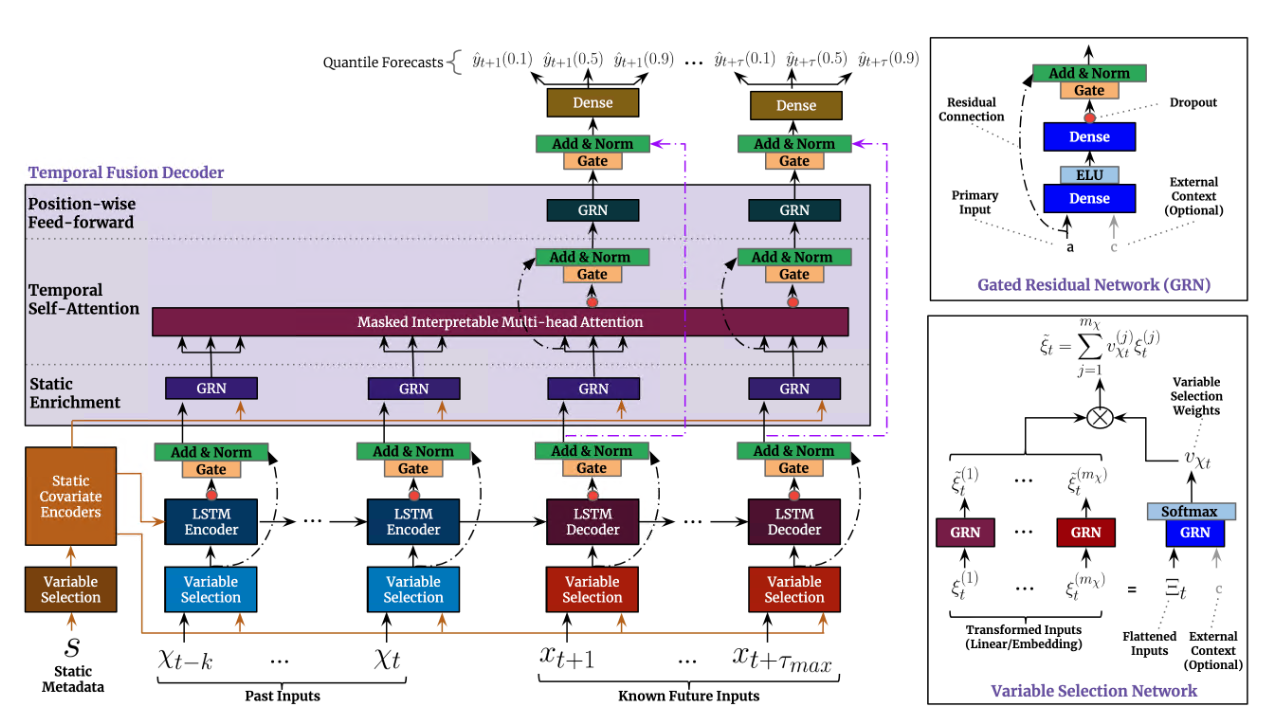
\includegraphics[keepaspectratio]{src/tft.png}}
\caption{Overview of TFT model architecture}
\end{figure}

    \paragraph{Implementation of Day-ahead Electricity Price
Forecasting}\label{implementation-of-day-ahead-electricity-price-forecasting}

Given its flexibility to consider multiple types of covariate
information, which foremost represent surrogates of supply and demand
(i.e.~weather forecasts, holidays, generation capacities and outages),
TFT is specially well suited for the forecasting of day-ahead
electricity prices. For this aim, the following variables are included
in the model:

\rowcolors{2}{white}{gray!25}
{\fontsize{8pt}{10pt}\selectfont\begin{longtable}[]{@{}
  >{\raggedright\arraybackslash}p{(\linewidth - 8\tabcolsep) * \real{0.1531}}
  >{\raggedright\arraybackslash}p{(\linewidth - 8\tabcolsep) * \real{0.1818}}
  >{\raggedright\arraybackslash}p{(\linewidth - 8\tabcolsep) * \real{0.0909}}
  >{\raggedright\arraybackslash}p{(\linewidth - 8\tabcolsep) * \real{0.0861}}
  >{\raggedright\arraybackslash}p{(\linewidth - 8\tabcolsep) * \real{0.4880}}@{}}
\toprule\noalign{}
\begin{minipage}[b]{\linewidth}\raggedright
Data variable
\end{minipage} & \begin{minipage}[b]{\linewidth}\raggedright
Variable type
\end{minipage} & \begin{minipage}[b]{\linewidth}\raggedright
Units
\end{minipage} & \begin{minipage}[b]{\linewidth}\raggedright
Source
\end{minipage} & \begin{minipage}[b]{\linewidth}\raggedright
Comments
\end{minipage} \\
\midrule\noalign{}
\endhead
\bottomrule\noalign{}
\endlastfoot
Electricity price & target predicted variable & EUR / MWh & ENTSO-E & \\
Day ahead forecast system load & time-varying known real input & MW &
ENTSO-E & Values are released hours before day ahead gate closure \\
Actual system load & time-varying unknown real input & MW & ENTSO-E & \\
Generation capacities & time-varying known real input & MW & ENTSO-E &
Capacities include known generation and production outages \\
Fossil-Fuel prices & time-varying known real input & EUR / MWh & Eikon
datastream & \\
Sunshine hours & time-varying unknown real input & minutes per hour &
DWD & Stations considered: Brocken, München Flughafen,
Hamburg-Fuhlsbüttel, Köln/Bonn, Leipzig/Halle \\
Wind speed & time-varying unknown real input & m/s & DWD & Stations
considered: Brocken, München Flughafen, Hamburg-Fuhlsbüttel, Köln/Bonn,
Leipzig/Halle \\
Holidays & time-varying known categorical input & NA & NA & Holiday
considering its name and each federal state \\
Date features & time-varying known real input & NA & NA & Encoded as
sine and cosine of hour of day, day of week and month of year \\
\end{longtable}}

    With this data considered, up to date our model has been trained
considering the timeframe from October 2018 (establishment of DE\_LU as
bidding zone) up to November 2024 (inclusive). Furthermore, day-ahead
forecasting tests have been conducted for all days of December 2024
achieving an average MAPE of 60.25 \% and an average MAE of 32.66
EUR/MWh. In this regard, extreme values for electricity prices took
place, specially given very low and high values for wind energy
generation, which along with solar generation, are indirectly considered
as unknown real inputs in this model. Below such forecast results are
depicted:

    \begin{figure}
\centering
{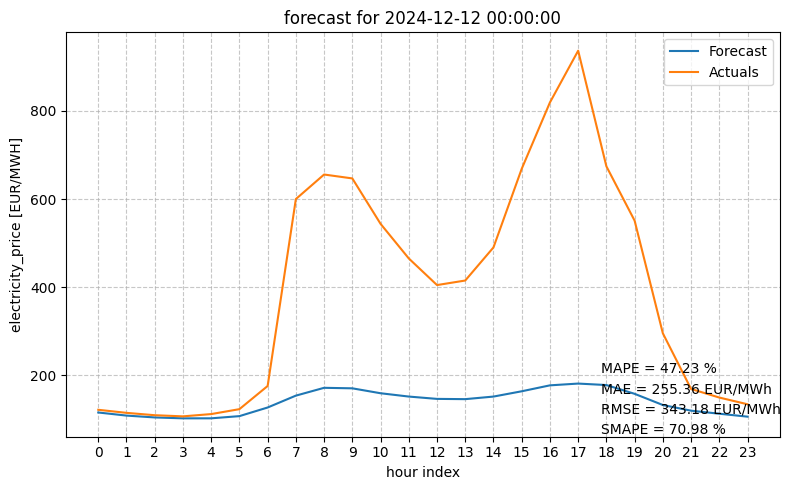
\includegraphics[keepaspectratio]{src/max_mae.png}}
\caption{Impact of ``Dunkelflaute'' on actual and predicted electricity
prices}
\end{figure}

    \begin{figure}
\centering
{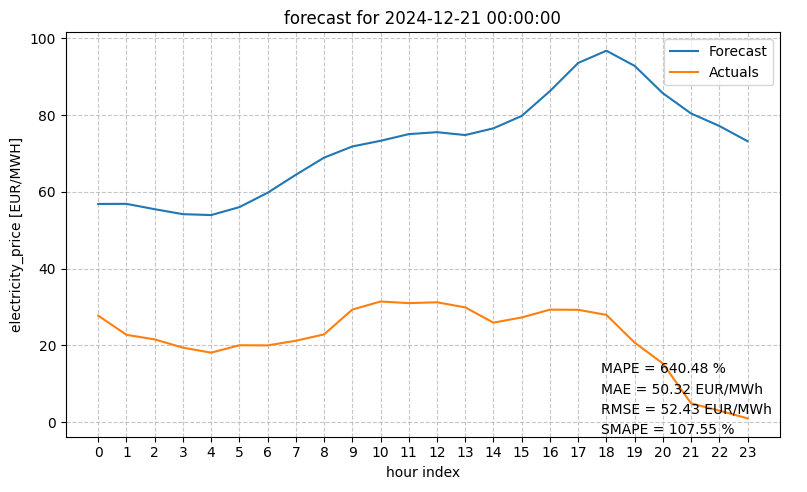
\includegraphics[keepaspectratio]{src/max_mape.png}}
\caption{Impact of renewable generation on actual and predicted
electricity prices}
\end{figure}

    It can be seen for instance, that for the 12th of December 2024, very
high electricity prices where experienced given a relative standstill in
wind and solar generation (so called ``Dunkelflaute''). In turn, for the
21st of December, large amounts of renewable generation took place, thus
driving electricity prices to quite low values.

Interestingly, the TFT model achieved relatively very good prediction
results for several days of this month. Below are two of thes cases:

    \begin{figure}
\centering
{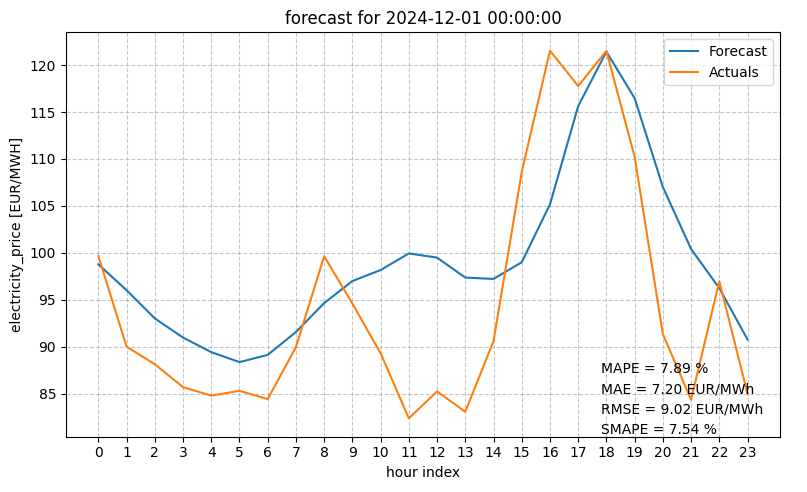
\includegraphics[keepaspectratio]{src/min_mae.png}}
\caption{Actual vs predicted electricity prices on 2025-12-01}
\end{figure}

    \begin{figure}
\centering
{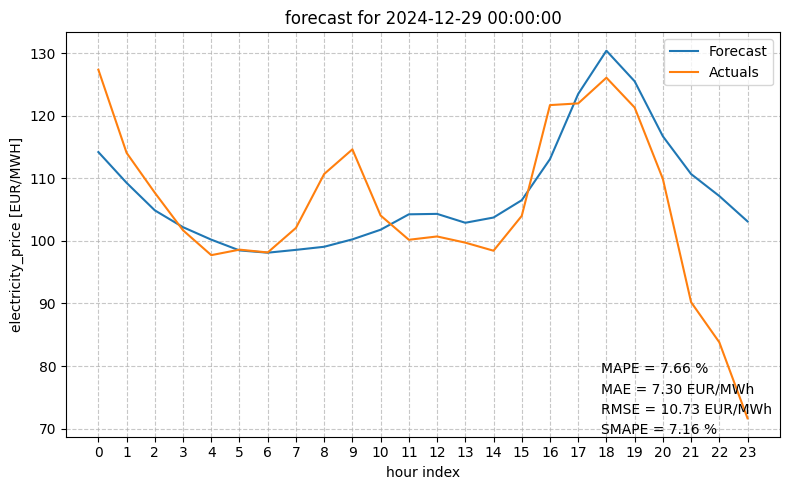
\includegraphics[keepaspectratio]{src/min_mape.png}}
\caption{Actual vs predicted electricity prices on 2025-12-29}
\end{figure}

    \subsection{AutoGluon}\label{autogluon}

    For our final approach, we also used the open-source AutoML library
AutoGluon (AG). AG has three modes of operation: Tabular, Multimodal,
and Time Series. In our predictions, Time Series Forecasting is used, as
it can forecast future values of multiple time series when given
previous data. Since chosing a model for forecasting can be difficult
and depends heavily on the given data, AG can run forecasts with many
different models. This approach avoids testing every model individually
and also prevents bias toward better-known models. The number of models
tested and their hyperparameters can be selected separately for each
implementation. Additionally, AutoGluon offers the option to combine
multiple models into a Weighted Ensemble model for potentially even
better results. AG compares the models with a given metric and at the
end, the forecast of the best model is the output. This means that AG
offers its users the ability to test multiple models and optimize the
results without much prior knowledge or manual testing{[}Shur et
al.~2023{]}.

We provided AG with our data frame and divided our features into three
categories: static data, known covariates, and past covariates.

\begin{itemize}
\item
  Static values: Data points like location that do not change over time;
  there is no such data point in our data frame.
\item
  Known covariates: Data points that are known for the future, e.g., day
  of the week, weather forecast, and holidays.
\item
  Past covariates: Data points that are not known in the future, e.g.,
  stock market values, cross-border energy flows.
\end{itemize}

As we have collected data from 2015 until now for around 150 model
inputs, it is a considerable amount of data and presents many challenges
for processing. Before running with the whole data frame, AG performs
its own preprocessing, e.g., too many NULL values or incompatible data
types. Another test is correlation between data points. If two data
points are too closely correlated, AG removes one from the calculations
to avoid spending unnecessary computation time. AG also automatically
checks if certain models require longer training time than allocated by
the user. In such cases, AG automatically skips training that model and
moves on to the next.

As mentioned above, AG trains several models by default but can also
train models specifically chosen by the user. These models range from
naive forecasts (which sets the forecast to the last observed value) to
Temporal Fusion Models and Chronos Models mentioned above. Since these
models do not need to be implemented separately, no decision needs to be
made in advance, and models can simply be chosen for their results at
the end. AG also provides a forecast using a Weighted Ensemble Model,
which takes the best-performing models from the training and combines
them for an even better forecast. Additionally, AG offers users the
opportunity to use different presets and hyperparameters for each model.
Presets range from medium\_quality to best\_quality, where the duration
of training increases significantly. Hyperparameters can be chosen for
each model separately, or AG can use default values.

The different models that were trained by AG and their results for the
validation score can be seen below. In that case, the weighted ensemble
approach had the best score. Additionally, the time for predictions
using the model and the fit time are given in seconds.

    \rowcolors{2}{white}{gray!25}
{\fontsize{8pt}{10pt}\selectfont\begin{longtable}[]{@{}
  >{\raggedright\arraybackslash}p{(\linewidth - 6\tabcolsep) * \real{0.4051}}
  >{\raggedright\arraybackslash}p{(\linewidth - 6\tabcolsep) * \real{0.1646}}
  >{\raggedright\arraybackslash}p{(\linewidth - 6\tabcolsep) * \real{0.1899}}
  >{\raggedright\arraybackslash}p{(\linewidth - 6\tabcolsep) * \real{0.2405}}@{}}
\toprule\noalign{}
\begin{minipage}[b]{\linewidth}\raggedright
Model
\end{minipage} & \begin{minipage}[b]{\linewidth}\raggedright
Score Val
\end{minipage} & \begin{minipage}[b]{\linewidth}\raggedright
Pred Time Val
\end{minipage} & \begin{minipage}[b]{\linewidth}\raggedright
Fit Time Marginal
\end{minipage} \\
\midrule\noalign{}
\endhead
\bottomrule\noalign{}
\endlastfoot
WeightedEnsemble & -0.038 & 57.56 & 0.08 \\
TemporalFusion Transformer & -0.047 & 0.04 & 338.58 \\
TiDE & -0.061 & 0.02 & 718.89 \\
Chronos Fine Tuned {[}bolt\_small{]} & -0.079 & 0.03 & 81.40 \\
ChronosZeroShot{[}bolt\_base{]} & -0.084 & 28.90 & 39.93 \\
DirectTabular & -0.090 & 0.09 & 43.85 \\
PatchTST & -0.096 & 0.02 & 79.90 \\
DeepAR & -0.104 & 0.10 & 222.96 \\
Recursive Tabular & -0.125 & 0.21 & 9.54 \\
SeasonalNaive & -0.128 & 15.61 & 0.03 \\
AutoETS & -0.150 & 4.47 & 0.12 \\
DynamicOptimizedTheta & -0.171 & 50.40 & 0.11 \\
NPTS & -0.244 & 2.65 & 0.03 \\
\end{longtable}}

    \paragraph{Start Basic Autogluon Code}\label{start-basic-autogluon-code}

    \begin{tcolorbox}[breakable, size=fbox, boxrule=1pt, pad at break*=1mm,colback=cellbackground, colframe=cellborder]
\prompt{In}{incolor}{ }{\boxspacing}
\begin{small}
\begin{Verbatim}[commandchars=\\\{\}]
\PY{n}{preset\PYZus{}list} \PY{o}{=} \PY{p}{[}\PY{l+s+s2}{\PYZdq{}}\PY{l+s+s2}{high\PYZus{}quality}\PY{l+s+s2}{\PYZdq{}}\PY{p}{,} \PY{l+s+s2}{\PYZdq{}}\PY{l+s+s2}{best\PYZus{}quality}\PY{l+s+s2}{\PYZdq{}}\PY{p}{,} \PY{l+s+s2}{\PYZdq{}}\PY{l+s+s2}{fast\PYZus{}training}\PY{l+s+s2}{\PYZdq{}}\PY{p}{,} \PY{l+s+s2}{\PYZdq{}}\PY{l+s+s2}{medium\PYZus{}quality}\PY{l+s+s2}{\PYZdq{}}\PY{p}{,} \PY{l+s+s2}{\PYZdq{}}\PY{l+s+s2}{hp1}\PY{l+s+s2}{\PYZdq{}}\PY{p}{]}
\PY{n}{set\PYZus{}time\PYZus{}limit} \PY{o}{=} \PY{k+kc}{None}
\PY{n}{output\PYZus{}folder\PYZus{}autogluon} \PY{o}{=} \PY{l+s+sa}{f}\PY{l+s+s2}{\PYZdq{}}\PY{l+s+s2}{/data/horse/ws/fewa833b\PYZhy{}time\PYZhy{}series\PYZhy{}forecast/AutoGluon/Felix/AllInOne}\PY{l+s+s2}{\PYZdq{}}

\PY{c+c1}{\PYZsh{}Start baseline}
\PY{n}{dataset} \PY{o}{=} \PY{l+s+s1}{\PYZsq{}}\PY{l+s+s1}{dayhead}\PY{l+s+s1}{\PYZsq{}}
\PY{n}{loaded\PYZus{}dataframe}\PY{p}{,} \PY{n}{file\PYZus{}path}\PY{p}{,} \PY{n}{data} \PY{o}{=} \PY{n}{dataset\PYZus{}Setup}\PY{p}{(}\PY{n}{dataset}\PY{p}{)}
\PY{n}{correlation\PYZus{}output\PYZus{}folder} \PY{o}{=} \PY{n}{os}\PY{o}{.}\PY{n}{path}\PY{o}{.}\PY{n}{join}\PY{p}{(}\PY{n}{output\PYZus{}folder\PYZus{}autogluon}\PY{p}{,} \PY{l+s+s2}{\PYZdq{}}\PY{l+s+s2}{Correlation}\PY{l+s+s2}{\PYZdq{}}\PY{p}{,} \PY{l+s+s2}{\PYZdq{}}\PY{l+s+s2}{Baseline}\PY{l+s+s2}{\PYZdq{}}\PY{p}{)}
\PY{n}{correlation\PYZus{}calculation}\PY{p}{(}\PY{n}{data}\PY{p}{,} \PY{n}{correlation\PYZus{}output\PYZus{}folder}\PY{p}{)}
\PY{n}{provide\PYZus{}known\PYZus{}covariables} \PY{o}{=} \PY{k+kc}{None}
\PY{n}{set\PYZus{}preset} \PY{o}{=} \PY{l+s+s2}{\PYZdq{}}\PY{l+s+s2}{fast\PYZus{}training}\PY{l+s+s2}{\PYZdq{}}
\PY{n}{train\PYZus{}autogluon}\PY{p}{(}\PY{n}{set\PYZus{}preset}\PY{p}{,} \PY{n}{set\PYZus{}time\PYZus{}limit}\PY{p}{,} \PY{n}{dataset}\PY{p}{,} \PY{n}{provide\PYZus{}known\PYZus{}covariables}\PY{p}{,} \PY{n}{output\PYZus{}folder\PYZus{}autogluon}\PY{p}{,}
                \PY{n}{loaded\PYZus{}dataframe}\PY{p}{,} \PY{n}{file\PYZus{}path}\PY{p}{,} \PY{n}{data}\PY{p}{)}

\PY{c+c1}{\PYZsh{}start all\PYZhy{}data}
\PY{n}{dataset} \PY{o}{=} \PY{l+s+s1}{\PYZsq{}}\PY{l+s+s1}{all}\PY{l+s+s1}{\PYZsq{}}
\PY{n}{correlation\PYZus{}output\PYZus{}folder} \PY{o}{=} \PY{n}{os}\PY{o}{.}\PY{n}{path}\PY{o}{.}\PY{n}{join}\PY{p}{(}\PY{n}{output\PYZus{}folder\PYZus{}autogluon}\PY{p}{,} \PY{l+s+s2}{\PYZdq{}}\PY{l+s+s2}{Correlation}\PY{l+s+s2}{\PYZdq{}}\PY{p}{,} \PY{l+s+s2}{\PYZdq{}}\PY{l+s+s2}{Less\PYZhy{}Data}\PY{l+s+s2}{\PYZdq{}}\PY{p}{)}
\PY{n}{correlation\PYZus{}calculation}\PY{p}{(}\PY{n}{data}\PY{p}{,} \PY{n}{correlation\PYZus{}output\PYZus{}folder}\PY{p}{)}
\PY{k}{for} \PY{n}{set\PYZus{}preset} \PY{o+ow}{in} \PY{n}{preset\PYZus{}list}\PY{p}{:}
    \PY{n}{provide\PYZus{}known\PYZus{}covariables} \PY{o}{=} \PY{k+kc}{None}
    \PY{n}{train\PYZus{}autogluon}\PY{p}{(}\PY{n}{set\PYZus{}preset}\PY{p}{,} \PY{n}{set\PYZus{}time\PYZus{}limit}\PY{p}{,} \PY{n}{dataset}\PY{p}{,} \PY{n}{provide\PYZus{}known\PYZus{}covariables}\PY{p}{,} \PY{n}{output\PYZus{}folder\PYZus{}autogluon}\PY{p}{,}
                    \PY{n}{loaded\PYZus{}dataframe}\PY{p}{,} \PY{n}{file\PYZus{}path}\PY{p}{,} \PY{n}{data}\PY{p}{)}

    \PY{n}{provide\PYZus{}known\PYZus{}covariables} \PY{o}{=} \PY{k+kc}{True}
    \PY{n}{train\PYZus{}autogluon}\PY{p}{(}\PY{n}{set\PYZus{}preset}\PY{p}{,} \PY{n}{set\PYZus{}time\PYZus{}limit}\PY{p}{,} \PY{n}{dataset}\PY{p}{,} \PY{n}{provide\PYZus{}known\PYZus{}covariables}\PY{p}{,} \PY{n}{output\PYZus{}folder\PYZus{}autogluon}\PY{p}{,}
                    \PY{n}{loaded\PYZus{}dataframe}\PY{p}{,} \PY{n}{file\PYZus{}path}\PY{p}{,} \PY{n}{data}\PY{p}{)}

\PY{c+c1}{\PYZsh{}start less\PYZhy{}data}
\PY{n}{dataset} \PY{o}{=} \PY{l+s+s2}{\PYZdq{}}\PY{l+s+s2}{less}\PY{l+s+s2}{\PYZdq{}}
\PY{n}{correlation\PYZus{}output\PYZus{}folder} \PY{o}{=} \PY{n}{os}\PY{o}{.}\PY{n}{path}\PY{o}{.}\PY{n}{join}\PY{p}{(}\PY{n}{output\PYZus{}folder\PYZus{}autogluon}\PY{p}{,} \PY{l+s+s2}{\PYZdq{}}\PY{l+s+s2}{Correlation}\PY{l+s+s2}{\PYZdq{}}\PY{p}{,} \PY{l+s+s2}{\PYZdq{}}\PY{l+s+s2}{Less\PYZhy{}Data}\PY{l+s+s2}{\PYZdq{}}\PY{p}{)}
\PY{n}{correlation\PYZus{}calculation}\PY{p}{(}\PY{n}{data}\PY{p}{,} \PY{n}{correlation\PYZus{}output\PYZus{}folder}\PY{p}{)}
\PY{k}{for} \PY{n}{set\PYZus{}preset} \PY{o+ow}{in} \PY{n}{preset\PYZus{}list}\PY{p}{:}
    \PY{n}{provide\PYZus{}known\PYZus{}covariables} \PY{o}{=} \PY{k+kc}{None}
    \PY{n}{train\PYZus{}autogluon}\PY{p}{(}\PY{n}{set\PYZus{}preset}\PY{p}{,} \PY{n}{set\PYZus{}time\PYZus{}limit}\PY{p}{,} \PY{n}{dataset}\PY{p}{,} \PY{n}{provide\PYZus{}known\PYZus{}covariables}\PY{p}{,} \PY{n}{output\PYZus{}folder\PYZus{}autogluon}\PY{p}{,}
                    \PY{n}{loaded\PYZus{}dataframe}\PY{p}{,} \PY{n}{file\PYZus{}path}\PY{p}{,} \PY{n}{data}\PY{p}{)}

    \PY{n}{provide\PYZus{}known\PYZus{}covariables} \PY{o}{=} \PY{k+kc}{True}
    \PY{n}{train\PYZus{}autogluon}\PY{p}{(}\PY{n}{set\PYZus{}preset}\PY{p}{,} \PY{n}{set\PYZus{}time\PYZus{}limit}\PY{p}{,} \PY{n}{dataset}\PY{p}{,} \PY{n}{provide\PYZus{}known\PYZus{}covariables}\PY{p}{,} \PY{n}{output\PYZus{}folder\PYZus{}autogluon}\PY{p}{,}
                    \PY{n}{loaded\PYZus{}dataframe}\PY{p}{,} \PY{n}{file\PYZus{}path}\PY{p}{,} \PY{n}{data}\PY{p}{)}
\end{Verbatim}
\end{small}
\end{tcolorbox}

    \subsection{Tuning AutoGluon}\label{tuning-autogluon}

In the AutoGluon group, an attempt was made to optimise the prediction
with AutoGluon by using different settings. The aim was to evaluate the
performance of different approaches and to analyse the importance of
additional data and external influencing factors. For this purpose,
different AutoGluon presets were used, including best\_quality,
fast\_training, high\_quality, medium\_quality and two customised
configurations with user-defined hyperparameters (hp1 and hp2). The
models were trained on two distinct datasets:

    \begin{enumerate}
\def\labelenumi{\arabic{enumi}.}
\tightlist
\item
  allData.csv: A comprehensive dataset with over 150 data points per
  hour, providing a detailed basis for more accurate predictions.
\item
  lessData.csv: A reduced data set with around 30 data points per hour,
  which represents whether the model can also make good predictions with
  less data
\end{enumerate}

As part of the investigation of the effects of external factors on the
prediction quality, the training runs were carried out in two variants.
In the first variant, known covariates such as the day (e.g.~weekday or
public holiday) and weather conditions (e.g.~temperature or
precipitation) were included in the modelling. In the second variant, on
the other hand, only the time stamps and the target value were used to
optimise the models.

To evaluate the effectiveness of the different approaches, a simple
baseline was used as a reference point, which only used the time and the
day-ahead price as input data. The aim was to determine the potential
improvements in forecast accuracy through additional data points.

    \begin{tcolorbox}[breakable, size=fbox, boxrule=1pt, pad at break*=1mm,colback=cellbackground, colframe=cellborder]
\prompt{In}{incolor}{7}{\boxspacing}
\begin{small}
\begin{Verbatim}[commandchars=\\\{\}]
\PY{k+kn}{import}\PY{+w}{ }\PY{n+nn}{matplotlib}\PY{n+nn}{.}\PY{n+nn}{pyplot}\PY{+w}{ }\PY{k}{as}\PY{+w}{ }\PY{n+nn}{plt}
\PY{k+kn}{import}\PY{+w}{ }\PY{n+nn}{pandas}\PY{+w}{ }\PY{k}{as}\PY{+w}{ }\PY{n+nn}{pd}

\PY{c+c1}{\PYZsh{} Read the CSV file into a pandas DataFrame}
\PY{n}{file\PYZus{}path} \PY{o}{=} \PY{l+s+s2}{\PYZdq{}}\PY{l+s+s2}{temp/preset\PYZhy{}comparison.csv}\PY{l+s+s2}{\PYZdq{}}
\PY{n}{df} \PY{o}{=} \PY{n}{pd}\PY{o}{.}\PY{n}{read\PYZus{}csv}\PY{p}{(}\PY{n}{file\PYZus{}path}\PY{p}{)}

\PY{c+c1}{\PYZsh{} Ensure \PYZsq{}Knowncoavariables\PYZsq{} is treated as a string and replace NaN or empty values with \PYZsq{}False\PYZsq{}}
\PY{n}{df}\PY{p}{[}\PY{l+s+s1}{\PYZsq{}}\PY{l+s+s1}{Knowncoavariables}\PY{l+s+s1}{\PYZsq{}}\PY{p}{]} \PY{o}{=} \PY{n}{df}\PY{p}{[}\PY{l+s+s1}{\PYZsq{}}\PY{l+s+s1}{Knowncoavariables}\PY{l+s+s1}{\PYZsq{}}\PY{p}{]}\PY{o}{.}\PY{n}{fillna}\PY{p}{(}\PY{l+s+s1}{\PYZsq{}}\PY{l+s+s1}{False}\PY{l+s+s1}{\PYZsq{}}\PY{p}{)}\PY{o}{.}\PY{n}{astype}\PY{p}{(}\PY{n+nb}{str}\PY{p}{)}

\PY{c+c1}{\PYZsh{} Create bar labels: Modelpreset\PYZus{}Dataset\PYZus{}Knowncoavariables}
\PY{n}{df}\PY{p}{[}\PY{l+s+s1}{\PYZsq{}}\PY{l+s+s1}{Labels}\PY{l+s+s1}{\PYZsq{}}\PY{p}{]} \PY{o}{=} \PY{n}{df}\PY{p}{[}\PY{l+s+s1}{\PYZsq{}}\PY{l+s+s1}{Modelpreset}\PY{l+s+s1}{\PYZsq{}}\PY{p}{]} \PY{o}{+} \PY{l+s+s1}{\PYZsq{}}\PY{l+s+s1}{\PYZus{}}\PY{l+s+s1}{\PYZsq{}} \PY{o}{+} \PY{n}{df}\PY{p}{[}\PY{l+s+s1}{\PYZsq{}}\PY{l+s+s1}{Dataset}\PY{l+s+s1}{\PYZsq{}}\PY{p}{]} \PY{o}{+} \PY{l+s+s1}{\PYZsq{}}\PY{l+s+s1}{\PYZus{}}\PY{l+s+s1}{\PYZsq{}} \PY{o}{+} \PY{n}{df}\PY{p}{[}\PY{l+s+s1}{\PYZsq{}}\PY{l+s+s1}{Knowncoavariables}\PY{l+s+s1}{\PYZsq{}}\PY{p}{]}

\PY{c+c1}{\PYZsh{} Create the plot}
\PY{n}{fig}\PY{p}{,} \PY{n}{ax} \PY{o}{=} \PY{n}{plt}\PY{o}{.}\PY{n}{subplots}\PY{p}{(}\PY{l+m+mi}{2}\PY{p}{,} \PY{l+m+mi}{1}\PY{p}{,} \PY{n}{figsize}\PY{o}{=}\PY{p}{(}\PY{l+m+mi}{10}\PY{p}{,} \PY{l+m+mi}{8}\PY{p}{)}\PY{p}{)}

\PY{c+c1}{\PYZsh{} MAE Plot}
\PY{n}{colors\PYZus{}mae} \PY{o}{=} \PY{p}{[}\PY{l+s+s1}{\PYZsq{}}\PY{l+s+s1}{blue}\PY{l+s+s1}{\PYZsq{}} \PY{k}{if} \PY{n}{value} \PY{o}{!=} \PY{n}{df}\PY{p}{[}\PY{l+s+s1}{\PYZsq{}}\PY{l+s+s1}{MAE SKlearn}\PY{l+s+s1}{\PYZsq{}}\PY{p}{]}\PY{o}{.}\PY{n}{min}\PY{p}{(}\PY{p}{)} \PY{k}{else} \PY{l+s+s1}{\PYZsq{}}\PY{l+s+s1}{red}\PY{l+s+s1}{\PYZsq{}} \PY{k}{for} \PY{n}{value} \PY{o+ow}{in} \PY{n}{df}\PY{p}{[}\PY{l+s+s1}{\PYZsq{}}\PY{l+s+s1}{MAE SKlearn}\PY{l+s+s1}{\PYZsq{}}\PY{p}{]}\PY{p}{]}
\PY{n}{ax}\PY{p}{[}\PY{l+m+mi}{0}\PY{p}{]}\PY{o}{.}\PY{n}{bar}\PY{p}{(}\PY{n}{df}\PY{p}{[}\PY{l+s+s1}{\PYZsq{}}\PY{l+s+s1}{Labels}\PY{l+s+s1}{\PYZsq{}}\PY{p}{]}\PY{p}{,} \PY{n}{df}\PY{p}{[}\PY{l+s+s1}{\PYZsq{}}\PY{l+s+s1}{MAE SKlearn}\PY{l+s+s1}{\PYZsq{}}\PY{p}{]}\PY{p}{,} \PY{n}{color}\PY{o}{=}\PY{n}{colors\PYZus{}mae}\PY{p}{,} \PY{n}{alpha}\PY{o}{=}\PY{l+m+mf}{0.7}\PY{p}{)}
\PY{n}{ax}\PY{p}{[}\PY{l+m+mi}{0}\PY{p}{]}\PY{o}{.}\PY{n}{set\PYZus{}title}\PY{p}{(}\PY{l+s+s1}{\PYZsq{}}\PY{l+s+s1}{Mean Absolute Error (MAE)}\PY{l+s+s1}{\PYZsq{}}\PY{p}{)}
\PY{n}{ax}\PY{p}{[}\PY{l+m+mi}{0}\PY{p}{]}\PY{o}{.}\PY{n}{set\PYZus{}ylabel}\PY{p}{(}\PY{l+s+s1}{\PYZsq{}}\PY{l+s+s1}{MAE}\PY{l+s+s1}{\PYZsq{}}\PY{p}{)}
\PY{n}{ax}\PY{p}{[}\PY{l+m+mi}{0}\PY{p}{]}\PY{o}{.}\PY{n}{set\PYZus{}xticklabels}\PY{p}{(}\PY{n}{df}\PY{p}{[}\PY{l+s+s1}{\PYZsq{}}\PY{l+s+s1}{Labels}\PY{l+s+s1}{\PYZsq{}}\PY{p}{]}\PY{p}{,} \PY{n}{rotation}\PY{o}{=}\PY{l+m+mi}{45}\PY{p}{,} \PY{n}{ha}\PY{o}{=}\PY{l+s+s1}{\PYZsq{}}\PY{l+s+s1}{right}\PY{l+s+s1}{\PYZsq{}}\PY{p}{)}


\PY{c+c1}{\PYZsh{} RMSE Plot}
\PY{n}{colors\PYZus{}rmse} \PY{o}{=} \PY{p}{[}\PY{l+s+s1}{\PYZsq{}}\PY{l+s+s1}{green}\PY{l+s+s1}{\PYZsq{}} \PY{k}{if} \PY{n}{value} \PY{o}{!=} \PY{n}{df}\PY{p}{[}\PY{l+s+s1}{\PYZsq{}}\PY{l+s+s1}{RMSE SKlearn}\PY{l+s+s1}{\PYZsq{}}\PY{p}{]}\PY{o}{.}\PY{n}{min}\PY{p}{(}\PY{p}{)} \PY{k}{else} \PY{l+s+s1}{\PYZsq{}}\PY{l+s+s1}{red}\PY{l+s+s1}{\PYZsq{}} \PY{k}{for} \PY{n}{value} \PY{o+ow}{in} \PY{n}{df}\PY{p}{[}\PY{l+s+s1}{\PYZsq{}}\PY{l+s+s1}{RMSE SKlearn}\PY{l+s+s1}{\PYZsq{}}\PY{p}{]}\PY{p}{]}
\PY{n}{ax}\PY{p}{[}\PY{l+m+mi}{1}\PY{p}{]}\PY{o}{.}\PY{n}{bar}\PY{p}{(}\PY{n}{df}\PY{p}{[}\PY{l+s+s1}{\PYZsq{}}\PY{l+s+s1}{Labels}\PY{l+s+s1}{\PYZsq{}}\PY{p}{]}\PY{p}{,} \PY{n}{df}\PY{p}{[}\PY{l+s+s1}{\PYZsq{}}\PY{l+s+s1}{RMSE SKlearn}\PY{l+s+s1}{\PYZsq{}}\PY{p}{]}\PY{p}{,} \PY{n}{color}\PY{o}{=}\PY{n}{colors\PYZus{}rmse}\PY{p}{,} \PY{n}{alpha}\PY{o}{=}\PY{l+m+mf}{0.7}\PY{p}{)}
\PY{n}{ax}\PY{p}{[}\PY{l+m+mi}{1}\PY{p}{]}\PY{o}{.}\PY{n}{set\PYZus{}title}\PY{p}{(}\PY{l+s+s1}{\PYZsq{}}\PY{l+s+s1}{Root Mean Squared Error (RMSE)}\PY{l+s+s1}{\PYZsq{}}\PY{p}{)}
\PY{n}{ax}\PY{p}{[}\PY{l+m+mi}{1}\PY{p}{]}\PY{o}{.}\PY{n}{set\PYZus{}ylabel}\PY{p}{(}\PY{l+s+s1}{\PYZsq{}}\PY{l+s+s1}{RMSE}\PY{l+s+s1}{\PYZsq{}}\PY{p}{)}
\PY{n}{ax}\PY{p}{[}\PY{l+m+mi}{1}\PY{p}{]}\PY{o}{.}\PY{n}{set\PYZus{}xticklabels}\PY{p}{(}\PY{n}{df}\PY{p}{[}\PY{l+s+s1}{\PYZsq{}}\PY{l+s+s1}{Labels}\PY{l+s+s1}{\PYZsq{}}\PY{p}{]}\PY{p}{,} \PY{n}{rotation}\PY{o}{=}\PY{l+m+mi}{45}\PY{p}{,} \PY{n}{ha}\PY{o}{=}\PY{l+s+s1}{\PYZsq{}}\PY{l+s+s1}{right}\PY{l+s+s1}{\PYZsq{}}\PY{p}{)}

\PY{c+c1}{\PYZsh{} Adjust layout to avoid overlapping}
\PY{n}{plt}\PY{o}{.}\PY{n}{tight\PYZus{}layout}\PY{p}{(}\PY{p}{)}
\PY{n}{plt}\PY{o}{.}\PY{n}{show}\PY{p}{(}\PY{p}{)}
\end{Verbatim}
\end{small}
\end{tcolorbox}

    \begin{center}
    \adjustimage{max size={0.9\linewidth}{0.9\paperheight}}{output_145_0.png}
    \end{center}
    { \hspace*{\fill} \\}
    
    The results for the different model variants are represented in the plot
above. The red columns represent the best models for the given error
metric, MAE and RMSE. Our best model for the MAE metric is
``high\_quality\_less\_False'', which means that the model used high
quality as a preset with the smaller dataset and no known covariants.
For RMSE the best models are ``best\_quality\_all\_False'' and
``high\_quality\_all\_False''. The full results can be found in the
table below.

    \rowcolors{2}{white}{gray!25}
{\fontsize{8pt}{10pt}\selectfont\begin{longtable}[]{@{}
  >{\raggedright\arraybackslash}p{(\linewidth - 10\tabcolsep) * \real{0.1235}}
  >{\raggedright\arraybackslash}p{(\linewidth - 10\tabcolsep) * \real{0.1852}}
  >{\raggedright\arraybackslash}p{(\linewidth - 10\tabcolsep) * \real{0.2222}}
  >{\raggedright\arraybackslash}p{(\linewidth - 10\tabcolsep) * \real{0.1605}}
  >{\raggedright\arraybackslash}p{(\linewidth - 10\tabcolsep) * \real{0.1728}}
  >{\raggedright\arraybackslash}p{(\linewidth - 10\tabcolsep) * \real{0.1358}}@{}}
\toprule\noalign{}
\begin{minipage}[b]{\linewidth}\raggedright
Dataset
\end{minipage} & \begin{minipage}[b]{\linewidth}\raggedright
Modelpreset
\end{minipage} & \begin{minipage}[b]{\linewidth}\raggedright
Known\hspace{0pt}covariables
\end{minipage} & \begin{minipage}[b]{\linewidth}\raggedright
MAE SKlearn
\end{minipage} & \begin{minipage}[b]{\linewidth}\raggedright
RMSE SKlearn
\end{minipage} & \begin{minipage}[b]{\linewidth}\raggedright
Duration
\end{minipage} \\
\midrule\noalign{}
\endhead
\bottomrule\noalign{}
\endlastfoot
less & high\_quality & & 19.53 & 33.23 & 5154.46 \\
less & best\_quality & & 19.57 & 33.27 & 5080.50 \\
less & high\_quality & True & 19.58 & 33.32 & 7029.28 \\
less & best\_quality & True & 19.63 & 33.31 & 12851.59 \\
all & high\_quality & & 20.32 & 33.08 & 2983.92 \\
all & best\_quality & & 20.32 & 33.08 & 3000.14 \\
all & high\_quality & True & 20.41 & 33.20 & 3051.78 \\
all & best\_quality & True & 20.41 & 33.20 & 3009.79 \\
all & medium\_quality & True & 21.12 & 34.47 & 1446.24 \\
all & medium\_quality & & 21.12 & 34.47 & 1460.18 \\
all & hp1 & & 22.03 & 35.50 & 2766.88 \\
all & hp1 & True & 22.03 & 35.51 & 2757.89 \\
less & hp1 & True & 22.16 & 35.44 & 2023.04 \\
less & hp1 & & 22.16 & 35.44 & 2105.08 \\
less & fast\_training & & 25.17 & 38.68 & 2621.76 \\
all & fast\_training & True & 25.17 & 38.68 & 6533.26 \\
all & fast\_training & & 25.17 & 38.68 & 6936.63 \\
less & fast\_training & True & 25.17 & 38.68 & 6740.39 \\
dayhead & fast\_training & True & 25.17 & 38.68 & 6910.75 \\
dayhead & fast\_training & & 25.17 & 38.68 & 7143.28 \\
\end{longtable}}

    Furthermore, an analysis was conducted to determine the extent to which
the selection of presets affects the computing time and the outcomes
obtained. The investigation focused on whether less complex presets,
such as fast\_training, could achieve results in a significantly shorter
time while maintaining a marginally lower level of accuracy under
specific conditions. This trade-off between computing time and model
performance is of particular relevance when models are updated with
additional data at a later stage to enhance resource efficiency.
However, this hypothesis could not be substantiated within the scope of
the present study.

In our results, the preset for fast\_training consistently produced
worse outcomes and required more training time than other model types.
In the plot below, our results are compared to the training duration of
each model. While fast\_training can be ruled out, the best\_quality
preset performs better while also having a shorter runtime.

    \begin{tcolorbox}[breakable, size=fbox, boxrule=1pt, pad at break*=1mm,colback=cellbackground, colframe=cellborder]
\prompt{In}{incolor}{8}{\boxspacing}
\begin{small}
\begin{Verbatim}[commandchars=\\\{\}]
\PY{k+kn}{import}\PY{+w}{ }\PY{n+nn}{pandas}\PY{+w}{ }\PY{k}{as}\PY{+w}{ }\PY{n+nn}{pd}
\PY{k+kn}{import}\PY{+w}{ }\PY{n+nn}{matplotlib}\PY{n+nn}{.}\PY{n+nn}{pyplot}\PY{+w}{ }\PY{k}{as}\PY{+w}{ }\PY{n+nn}{plt}
\PY{k+kn}{import}\PY{+w}{ }\PY{n+nn}{numpy}\PY{+w}{ }\PY{k}{as}\PY{+w}{ }\PY{n+nn}{np}

\PY{n}{file\PYZus{}path} \PY{o}{=} \PY{l+s+s2}{\PYZdq{}}\PY{l+s+s2}{temp/preset\PYZhy{}comparison.csv}\PY{l+s+s2}{\PYZdq{}}
\PY{n}{df} \PY{o}{=} \PY{n}{pd}\PY{o}{.}\PY{n}{read\PYZus{}csv}\PY{p}{(}\PY{n}{file\PYZus{}path}\PY{p}{)}
\PY{n}{df}\PY{p}{[}\PY{l+s+s1}{\PYZsq{}}\PY{l+s+s1}{Knowncoavariables}\PY{l+s+s1}{\PYZsq{}}\PY{p}{]} \PY{o}{=} \PY{n}{df}\PY{p}{[}\PY{l+s+s1}{\PYZsq{}}\PY{l+s+s1}{Knowncoavariables}\PY{l+s+s1}{\PYZsq{}}\PY{p}{]}\PY{o}{.}\PY{n}{apply}\PY{p}{(}\PY{k}{lambda} \PY{n}{x}\PY{p}{:} \PY{l+s+s1}{\PYZsq{}}\PY{l+s+s1}{true}\PY{l+s+s1}{\PYZsq{}} \PY{k}{if} \PY{n}{x} \PY{o+ow}{is} \PY{k+kc}{True} \PY{k}{else} \PY{l+s+s1}{\PYZsq{}}\PY{l+s+s1}{\PYZsq{}}\PY{p}{)}

\PY{k}{if} \PY{n}{df}\PY{p}{[}\PY{l+s+s1}{\PYZsq{}}\PY{l+s+s1}{MAE SKlearn}\PY{l+s+s1}{\PYZsq{}}\PY{p}{]}\PY{o}{.}\PY{n}{dtype} \PY{o}{==} \PY{n+nb}{object}\PY{p}{:}  \PY{c+c1}{\PYZsh{} If the column is of object type (strings)}
    \PY{n}{df}\PY{p}{[}\PY{l+s+s1}{\PYZsq{}}\PY{l+s+s1}{MAE SKlearn}\PY{l+s+s1}{\PYZsq{}}\PY{p}{]} \PY{o}{=} \PY{n}{df}\PY{p}{[}\PY{l+s+s1}{\PYZsq{}}\PY{l+s+s1}{MAE SKlearn}\PY{l+s+s1}{\PYZsq{}}\PY{p}{]}\PY{o}{.}\PY{n}{str}\PY{o}{.}\PY{n}{replace}\PY{p}{(}\PY{l+s+s1}{\PYZsq{}}\PY{l+s+s1}{\PYZpc{}}\PY{l+s+s1}{\PYZsq{}}\PY{p}{,} \PY{l+s+s1}{\PYZsq{}}\PY{l+s+s1}{\PYZsq{}}\PY{p}{)}\PY{o}{.}\PY{n}{astype}\PY{p}{(}\PY{n+nb}{float}\PY{p}{)}

\PY{n}{df} \PY{o}{=} \PY{n}{df}\PY{o}{.}\PY{n}{sort\PYZus{}values}\PY{p}{(}\PY{n}{by}\PY{o}{=}\PY{l+s+s1}{\PYZsq{}}\PY{l+s+s1}{MAE SKlearn}\PY{l+s+s1}{\PYZsq{}}\PY{p}{)}

\PY{c+c1}{\PYZsh{} y\PYZhy{} and x\PYZhy{}axis}
\PY{n}{fig}\PY{p}{,} \PY{n}{ax1} \PY{o}{=} \PY{n}{plt}\PY{o}{.}\PY{n}{subplots}\PY{p}{(}\PY{n}{figsize}\PY{o}{=}\PY{p}{(}\PY{l+m+mi}{12}\PY{p}{,} \PY{l+m+mi}{6}\PY{p}{)}\PY{p}{)}
\PY{n}{x\PYZus{}positions} \PY{o}{=} \PY{n}{np}\PY{o}{.}\PY{n}{arange}\PY{p}{(}\PY{n+nb}{len}\PY{p}{(}\PY{n}{df}\PY{p}{)}\PY{p}{)}
\PY{n}{ax1}\PY{o}{.}\PY{n}{bar}\PY{p}{(}\PY{n}{x\PYZus{}positions} \PY{o}{\PYZhy{}} \PY{l+m+mf}{0.2}\PY{p}{,} \PY{n}{df}\PY{p}{[}\PY{l+s+s1}{\PYZsq{}}\PY{l+s+s1}{Duration}\PY{l+s+s1}{\PYZsq{}}\PY{p}{]}\PY{p}{,} \PY{n}{color}\PY{o}{=}\PY{l+s+s1}{\PYZsq{}}\PY{l+s+s1}{orange}\PY{l+s+s1}{\PYZsq{}}\PY{p}{,} \PY{n}{label}\PY{o}{=}\PY{l+s+s1}{\PYZsq{}}\PY{l+s+s1}{Duration (s)}\PY{l+s+s1}{\PYZsq{}}\PY{p}{,} \PY{n}{width}\PY{o}{=}\PY{l+m+mf}{0.4}\PY{p}{,} \PY{n}{alpha}\PY{o}{=}\PY{l+m+mf}{0.7}\PY{p}{)}
\PY{n}{ax1}\PY{o}{.}\PY{n}{set\PYZus{}xlabel}\PY{p}{(}\PY{l+s+s1}{\PYZsq{}}\PY{l+s+s1}{Preset}\PY{l+s+s1}{\PYZsq{}}\PY{p}{)}
\PY{n}{ax1}\PY{o}{.}\PY{n}{set\PYZus{}ylabel}\PY{p}{(}\PY{l+s+s1}{\PYZsq{}}\PY{l+s+s1}{Duration (seconds)}\PY{l+s+s1}{\PYZsq{}}\PY{p}{,} \PY{n}{color}\PY{o}{=}\PY{l+s+s1}{\PYZsq{}}\PY{l+s+s1}{orange}\PY{l+s+s1}{\PYZsq{}}\PY{p}{)}
\PY{n}{ax1}\PY{o}{.}\PY{n}{tick\PYZus{}params}\PY{p}{(}\PY{n}{axis}\PY{o}{=}\PY{l+s+s1}{\PYZsq{}}\PY{l+s+s1}{y}\PY{l+s+s1}{\PYZsq{}}\PY{p}{,} \PY{n}{labelcolor}\PY{o}{=}\PY{l+s+s1}{\PYZsq{}}\PY{l+s+s1}{orange}\PY{l+s+s1}{\PYZsq{}}\PY{p}{)}

\PY{c+c1}{\PYZsh{} y\PYZhy{}axis for MAE SKlearn}
\PY{n}{ax2} \PY{o}{=} \PY{n}{ax1}\PY{o}{.}\PY{n}{twinx}\PY{p}{(}\PY{p}{)}
\PY{n}{ax2}\PY{o}{.}\PY{n}{bar}\PY{p}{(}\PY{n}{x\PYZus{}positions} \PY{o}{+} \PY{l+m+mf}{0.2}\PY{p}{,} \PY{n}{df}\PY{p}{[}\PY{l+s+s1}{\PYZsq{}}\PY{l+s+s1}{MAE SKlearn}\PY{l+s+s1}{\PYZsq{}}\PY{p}{]}\PY{p}{,} \PY{n}{color}\PY{o}{=}\PY{l+s+s1}{\PYZsq{}}\PY{l+s+s1}{blue}\PY{l+s+s1}{\PYZsq{}}\PY{p}{,} \PY{n}{label}\PY{o}{=}\PY{l+s+s1}{\PYZsq{}}\PY{l+s+s1}{MAE SKlearn}\PY{l+s+s1}{\PYZsq{}}\PY{p}{,} \PY{n}{width}\PY{o}{=}\PY{l+m+mf}{0.4}\PY{p}{,} \PY{n}{alpha}\PY{o}{=}\PY{l+m+mf}{0.7}\PY{p}{)}
\PY{n}{ax2}\PY{o}{.}\PY{n}{set\PYZus{}ylabel}\PY{p}{(}\PY{l+s+s1}{\PYZsq{}}\PY{l+s+s1}{MAE SKlearn}\PY{l+s+s1}{\PYZsq{}}\PY{p}{,} \PY{n}{color}\PY{o}{=}\PY{l+s+s1}{\PYZsq{}}\PY{l+s+s1}{blue}\PY{l+s+s1}{\PYZsq{}}\PY{p}{)}
\PY{n}{ax2}\PY{o}{.}\PY{n}{tick\PYZus{}params}\PY{p}{(}\PY{n}{axis}\PY{o}{=}\PY{l+s+s1}{\PYZsq{}}\PY{l+s+s1}{y}\PY{l+s+s1}{\PYZsq{}}\PY{p}{,} \PY{n}{labelcolor}\PY{o}{=}\PY{l+s+s1}{\PYZsq{}}\PY{l+s+s1}{blue}\PY{l+s+s1}{\PYZsq{}}\PY{p}{)}

\PY{n}{ax2}\PY{o}{.}\PY{n}{set\PYZus{}ylim}\PY{p}{(}\PY{l+m+mi}{0}\PY{p}{,} \PY{n}{df}\PY{p}{[}\PY{l+s+s1}{\PYZsq{}}\PY{l+s+s1}{MAE SKlearn}\PY{l+s+s1}{\PYZsq{}}\PY{p}{]}\PY{o}{.}\PY{n}{max}\PY{p}{(}\PY{p}{)} \PY{o}{+} \PY{l+m+mi}{5}\PY{p}{)}

\PY{c+c1}{\PYZsh{} title and labels}
\PY{n}{ax1}\PY{o}{.}\PY{n}{set\PYZus{}xticks}\PY{p}{(}\PY{n}{x\PYZus{}positions}\PY{p}{)}
\PY{n}{ax1}\PY{o}{.}\PY{n}{set\PYZus{}xticklabels}\PY{p}{(}\PY{n}{df}\PY{p}{[}\PY{l+s+s1}{\PYZsq{}}\PY{l+s+s1}{Modelpreset}\PY{l+s+s1}{\PYZsq{}}\PY{p}{]} \PY{o}{+} \PY{l+s+s2}{\PYZdq{}}\PY{l+s+s2}{\PYZus{}}\PY{l+s+s2}{\PYZdq{}} \PY{o}{+} \PY{n}{df}\PY{p}{[}\PY{l+s+s1}{\PYZsq{}}\PY{l+s+s1}{Dataset}\PY{l+s+s1}{\PYZsq{}}\PY{p}{]} \PY{o}{+} \PY{l+s+s2}{\PYZdq{}}\PY{l+s+s2}{ }\PY{l+s+s2}{\PYZdq{}} \PY{o}{+} \PY{n}{df}\PY{p}{[}\PY{l+s+s1}{\PYZsq{}}\PY{l+s+s1}{Knowncoavariables}\PY{l+s+s1}{\PYZsq{}}\PY{p}{]}\PY{p}{,} \PY{n}{rotation}\PY{o}{=}\PY{l+m+mi}{45}\PY{p}{,} \PY{n}{ha}\PY{o}{=}\PY{l+s+s2}{\PYZdq{}}\PY{l+s+s2}{right}\PY{l+s+s2}{\PYZdq{}}\PY{p}{)}

\PY{n}{plt}\PY{o}{.}\PY{n}{title}\PY{p}{(}\PY{l+s+s1}{\PYZsq{}}\PY{l+s+s1}{Duration and MAE SKlearn by Preset}\PY{l+s+s1}{\PYZsq{}}\PY{p}{)}
\PY{n}{fig}\PY{o}{.}\PY{n}{tight\PYZus{}layout}\PY{p}{(}\PY{p}{)}
\PY{n}{plt}\PY{o}{.}\PY{n}{show}\PY{p}{(}\PY{p}{)}
\end{Verbatim}
\end{small}
\end{tcolorbox}

    \begin{center}
    \adjustimage{max size={0.9\linewidth}{0.9\paperheight}}{output_149_0.png}
    \end{center}
    { \hspace*{\fill} \\}
    
    

    \subsection{Experimental Approaches}\label{experimental-approaches}

\paragraph{Leveraging News Embeddings}\label{leveraging-news-embeddings}

For evaluating the influence of the news embeddings on predicting the
day ahead price, we tested three configurations over a 30-day period:

\rowcolors{2}{white}{gray!25}
{\fontsize{8pt}{10pt}\selectfont\begin{longtable}[]{@{}ll@{}}
\toprule\noalign{}
Model Configuration & Validation RMSE \\
\midrule\noalign{}
\endhead
\bottomrule\noalign{}
\endlastfoot
NewsAPI embeddings + day-ahead + target & 28.82 \\
Guardian embeddings + day-ahead + target & 27.36 \\
Day-ahead + target (baseline) & 27.86 \\
\end{longtable}}

Using The Guardian's historical data, we extended the experiment to 10
years:

\rowcolors{2}{white}{gray!25}
{\fontsize{8pt}{10pt}\selectfont\begin{longtable}[]{@{}ll@{}}
\toprule\noalign{}
Model Configuration & Test RMSE \\
\midrule\noalign{}
\endhead
\bottomrule\noalign{}
\endlastfoot
Guardian embeddings + day-ahead (386 dimensions) & 73.88 \\
Guardian embeddings + day-ahead (PCA 8 dimensions) & 29.09 \\
Day-ahead + target (baseline) & 22.18 \\
\end{longtable}}

The results show that news embeddings did not improve the prediction of
German day-ahead prices. Future work should focus on finding more
relevant news sources for the German market and exploring more complex
model architectures that can better handle the embedding data.

    \begin{tcolorbox}[breakable, size=fbox, boxrule=1pt, pad at break*=1mm,colback=cellbackground, colframe=cellborder]
\prompt{In}{incolor}{13}{\boxspacing}
\begin{small}
\begin{Verbatim}[commandchars=\\\{\}]
\PY{c+c1}{\PYZsh{} Example inference}

\PY{n}{guardian\PYZus{}embeddings\PYZus{}day\PYZus{}ahead}\PY{p}{,} \PY{n}{newsapi\PYZus{}embeddings\PYZus{}day\PYZus{}ahead}\PY{p}{,} \PY{n}{day\PYZus{}ahead\PYZus{}prices\PYZus{}for\PYZus{}prediction}\PY{p}{,} \PY{n}{ground\PYZus{}truth} \PY{o}{=} \PY{n}{prepare\PYZus{}embedding\PYZus{}data}\PY{p}{(}\PY{n}{guardian\PYZus{}embeddings}\PY{p}{,} \PY{n}{newsapi\PYZus{}embeddings}\PY{p}{,} \PY{n}{day\PYZus{}ahead\PYZus{}prices}\PY{p}{)}

\PY{n}{guardian\PYZus{}predictor\PYZus{}path} \PY{o}{=}  \PY{l+s+s2}{\PYZdq{}}\PY{l+s+s2}{models/models/guardian\PYZus{}embedding\PYZus{}model}\PY{l+s+s2}{\PYZdq{}}
\PY{n}{newsapi\PYZus{}predictor\PYZus{}path} \PY{o}{=} \PY{l+s+s2}{\PYZdq{}}\PY{l+s+s2}{models/models/newsapi\PYZus{}embedding\PYZus{}model}\PY{l+s+s2}{\PYZdq{}}
\PY{n}{no\PYZus{}embeddings\PYZus{}predictor\PYZus{}path} \PY{o}{=} \PY{l+s+s2}{\PYZdq{}}\PY{l+s+s2}{models/models/no\PYZus{}embeddings\PYZus{}model}\PY{l+s+s2}{\PYZdq{}}

\PY{n}{guardian\PYZus{}predictions} \PY{o}{=} \PY{n}{predict\PYZus{}embedding\PYZus{}data}\PY{p}{(}\PY{n}{guardian\PYZus{}predictor\PYZus{}path}\PY{p}{,} \PY{n}{guardian\PYZus{}embeddings\PYZus{}day\PYZus{}ahead}\PY{p}{)}
\PY{n}{newsapi\PYZus{}predictions} \PY{o}{=} \PY{n}{predict\PYZus{}embedding\PYZus{}data}\PY{p}{(}\PY{n}{newsapi\PYZus{}predictor\PYZus{}path}\PY{p}{,} \PY{n}{newsapi\PYZus{}embeddings\PYZus{}day\PYZus{}ahead}\PY{p}{)}
\PY{n}{no\PYZus{}embeddings\PYZus{}predictions} \PY{o}{=} \PY{n}{predict\PYZus{}embedding\PYZus{}data}\PY{p}{(}\PY{n}{no\PYZus{}embeddings\PYZus{}predictor\PYZus{}path}\PY{p}{,} \PY{n}{day\PYZus{}ahead\PYZus{}prices\PYZus{}for\PYZus{}prediction}\PY{p}{)}

\PY{n}{visualize\PYZus{}embedding\PYZus{}model\PYZus{}results}\PY{p}{(}\PY{n}{guardian\PYZus{}predictions}\PY{p}{,} \PY{n}{ground\PYZus{}truth}\PY{p}{,} \PY{l+s+s2}{\PYZdq{}}\PY{l+s+s2}{Guardian Embeddings}\PY{l+s+s2}{\PYZdq{}}\PY{p}{)}
\PY{n}{visualize\PYZus{}embedding\PYZus{}model\PYZus{}results}\PY{p}{(}\PY{n}{newsapi\PYZus{}predictions}\PY{p}{,} \PY{n}{ground\PYZus{}truth}\PY{p}{,} \PY{l+s+s2}{\PYZdq{}}\PY{l+s+s2}{NewsAPI Embedddings}\PY{l+s+s2}{\PYZdq{}}\PY{p}{)}
\PY{n}{visualize\PYZus{}embedding\PYZus{}model\PYZus{}results}\PY{p}{(}\PY{n}{no\PYZus{}embeddings\PYZus{}predictions}\PY{p}{,} \PY{n}{ground\PYZus{}truth}\PY{p}{,} \PY{l+s+s2}{\PYZdq{}}\PY{l+s+s2}{No Embeddings}\PY{l+s+s2}{\PYZdq{}}\PY{p}{)}
\end{Verbatim}
\end{small}
\end{tcolorbox}

    \begin{center}
    \adjustimage{max size={0.9\linewidth}{0.9\paperheight}}{output_152_0.png}
    \end{center}
    { \hspace*{\fill} \\}
    
    \begin{center}
    \adjustimage{max size={0.9\linewidth}{0.9\paperheight}}{output_152_1.png}
    \end{center}
    { \hspace*{\fill} \\}
    
    \begin{center}
    \adjustimage{max size={0.9\linewidth}{0.9\paperheight}}{output_152_2.png}
    \end{center}
    { \hspace*{\fill} \\}
    
    \paragraph{Predicting Intraday-Prices as Additional
Feature}\label{predicting-intraday-prices-as-additional-feature}

Besides day-ahead prices, which are the target value of this time series
forecast, electric energy is also traded on the more short-term Intraday
market. While in general they refer to the same underlying product,
there are cases in which the prices of day-ahead and intraday trades
differ significantly, as the intraday market will react more short-term
to unforeseen changes in supply and demand. These short-term differences
can for example be induced by

    \begin{itemize}
\tightlist
\item
  extreme weather conditions offsetting forecast and actual generation
  of renewables affecting supply
\item
  extreme weather conditions generating an unforeseen surge or decline
  in demand
\item
  unplanned power plant outages creating a lack of supply
\item
  short-term changes in balancing affecting supply
\end{itemize}

As Germany saw their share of renewables in power generation rise, the
role of intraday prices for demand regulation became increasingly
important. Therefore the ``gate closure'' of intraday trades, meaning
the time between end of trading and delivery, got shortened
significantly. In July 2015 it was changed from 45 to 30 minutes,
whereas nowadays it's down to five minutes, and allows for a high
reactivity to changes in supply and demand. \hyperref[bibliography]{[Smard, Großhandelspreise, 2024]}

Given our time series dataset with all features that resulted from data
gathering, we tried to predict the intraday price to use as an
additional feature in predicting the day-ahead price. If we were to
predict the intraday prices with high accuracy, this could possibly be
an important feature for improving the day-ahead prediction.

Data Sources: The open data sources for intraday electric energy prices
are unfortunately very limited, as in many cases stock market data are
sold for commercial data analysis. ``Netztransparenz'', which is an
information transparency platform by the four German transmission grid
operators, publishes a dataset with quarter-hourly intraday price
indices from 30th June 2020 to date. These values are calculated as
volume-weighted average of the last stock market orders over 500MW for
quarter-hourly electricity \hyperref[bibliography]{[Netztransparenz, Index-Ausgleichspreis, 2024]}. The dataset of Netztransparenz is to our knowledge the only
freely available dataset for German intraday electricity prices.

    To investigate the potential of using intraday prices as an additional
feature for day-ahead price prediction, a systematic approach was
followed, involving the prediction of intraday prices and their
integration into the day-ahead prediction.

Following table contains the original quarter-hourly intraday
electricity price data as downloaded from the source.

    \begin{tcolorbox}[breakable, size=fbox, boxrule=1pt, pad at break*=1mm,colback=cellbackground, colframe=cellborder]
\prompt{In}{incolor}{44}{\boxspacing}
\begin{small}
\begin{Verbatim}[commandchars=\\\{\}]
\PY{n}{pd}\PY{o}{.}\PY{n}{read\PYZus{}csv}\PY{p}{(}\PY{l+s+s1}{\PYZsq{}}\PY{l+s+s1}{../final\PYZhy{}submission/merged\PYZus{}data/data\PYZus{}collection/Intraday\PYZus{}prices\PYZus{}2020\PYZus{}2025\PYZus{}quarter\PYZus{}hourly.csv}\PY{l+s+s1}{\PYZsq{}}\PY{p}{)}\PY{o}{.}\PY{n}{head}\PY{p}{(}\PY{p}{)}
\end{Verbatim}
\end{small}
\end{tcolorbox}

            \begin{tcolorbox}[breakable, size=fbox, boxrule=.5pt, pad at break*=1mm, opacityfill=0]
\prompt{Out}{outcolor}{44}{\boxspacing}
\begin{small}
\begin{Verbatim}[commandchars=\\\{\}]
              datetime  intraday\_price\_EURO
0  2020-07-01 00:00:00                25.46
1  2020-07-01 00:15:00                29.26
2  2020-07-01 00:30:00                25.98
3  2020-07-01 00:45:00                26.14
4  2020-07-01 01:00:00                18.00
\end{Verbatim}
\end{small}
\end{tcolorbox}
        
    To maintain consistency with the day-ahead price data and simplify
analysis, the quarter-hourly intraday price data was aggregated into
hourly values. This was achieved by calculating the mean of the four
quarter-hourly values for each hour, resulting in a manageable dataset
with hourly intraday prices that could be used for model training and
prediction.

    \begin{tcolorbox}[breakable, size=fbox, boxrule=1pt, pad at break*=1mm,colback=cellbackground, colframe=cellborder]
\prompt{In}{incolor}{45}{\boxspacing}
\begin{small}
\begin{Verbatim}[commandchars=\\\{\}]
\PY{n}{pd}\PY{o}{.}\PY{n}{read\PYZus{}csv}\PY{p}{(}\PY{l+s+s1}{\PYZsq{}}\PY{l+s+s1}{../final\PYZhy{}submission/merged\PYZus{}data/data\PYZus{}collection/Intraday\PYZus{}prices\PYZus{}2020\PYZus{}2025\PYZus{}hourly.csv}\PY{l+s+s1}{\PYZsq{}}\PY{p}{)}\PY{o}{.}\PY{n}{head}\PY{p}{(}\PY{p}{)}
\end{Verbatim}
\end{small}
\end{tcolorbox}

            \begin{tcolorbox}[breakable, size=fbox, boxrule=.5pt, pad at break*=1mm, opacityfill=0]
\prompt{Out}{outcolor}{45}{\boxspacing}
\begin{small}
\begin{Verbatim}[commandchars=\\\{\}]
                 datetime  intraday\_price\_EURO
0  2020-07-01 00:00:00+00                26.71
1  2020-07-01 01:00:00+00                20.97
2  2020-07-01 02:00:00+00                31.07
3  2020-07-01 03:00:00+00                34.37
4  2020-07-01 04:00:00+00                43.11
\end{Verbatim}
\end{small}
\end{tcolorbox}
        
    When examining the data, some strong outliers were clearly visible.
Outliers in time series data can distort trends and affect model
performance. To address this, we used the z-score method, identifying
values exceeding three standard deviations from the mean. This approach
effectively detects anomalies while preserving the overall data
distribution. A total of 539 outliers were detected and replaced using a
forward-fill approach to maintain data continuity. The plot below
illustrates these detected anomalies over time, highlighting significant
fluctuations in intraday electricity prices throughout 2024.

\begin{figure}
\centering
{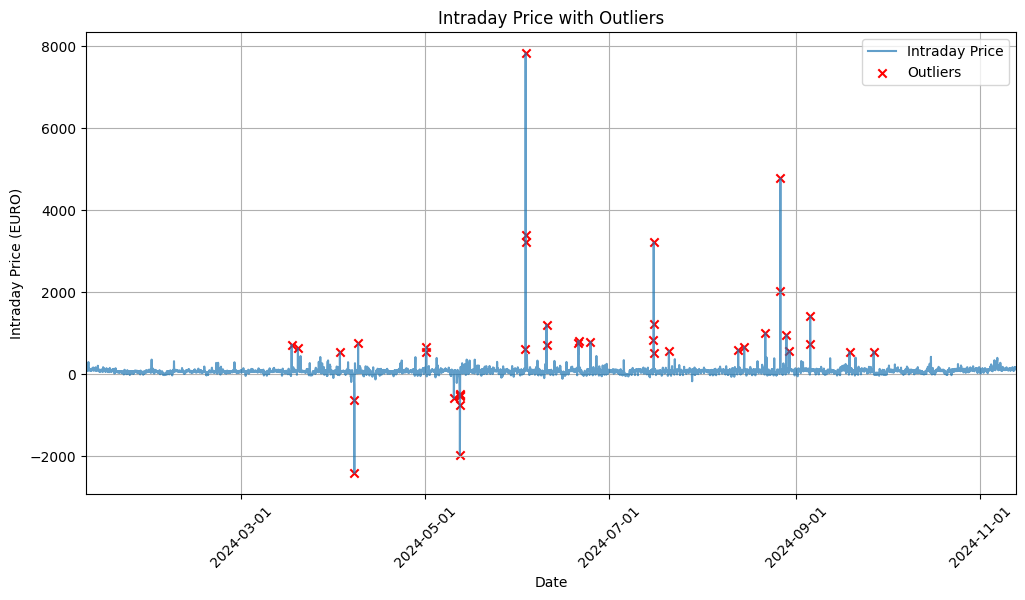
\includegraphics[keepaspectratio]{src/Intraday_price_outliers_2024_plot.png}}
\caption{Intraday price outliers in 2024}
\end{figure}

    Intraday prices were predicted for the same test set time intervals as
used for the day-ahead forecast. The models were trained using only the
\texttt{timestamp} and \texttt{intraday\_price\_EURO} columns. After
testing various configurations, the best results were obtained with the
``best\_quality'' preset using weighted\_ensemble.

\begin{figure}
\centering
{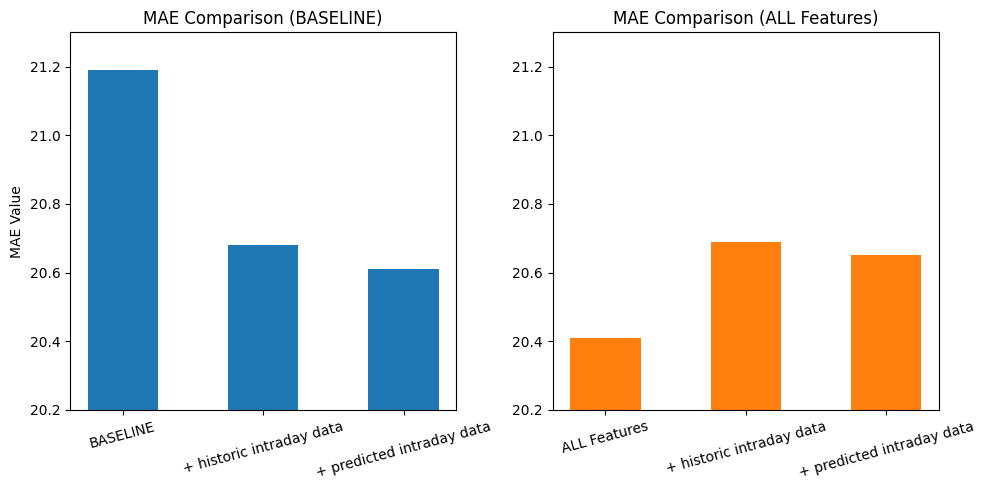
\includegraphics[keepaspectratio]{src/Intraday_price_comparison_plots.png}}
\caption{Comparison of dayahead price prediction accuracy with historic
and predicted intraday price as additional feature}
\end{figure}

The left chart above, labeled ``MAE Comparison (BASELINE)'', shows the
MAE for three different scenarios: the baseline model, the model
utilizing historical intraday data (assuming perfect predictions of
intraday prices), and the model combining both historical and predicted
intraday data. The baseline model shows the highest MAE, while both
additional features reduce the error, with predicted intraday data
yielding the lowest MAE in this comparison.

It is suggested that the slight decrease in prediction accuracy when
including historic intraday data compared to predicted intraday data is
caused by less outlying predicted values in average which have less
negative impact on the prediction accuracy but might not represent the
actual reality.

After showcasing the improvement in day-ahead predictions by integrating
intraday data into the baseline model, we investigated its impact on the
full dataset, which includes all available features, to evaluate its
relevance for the project. As demonstrated in the chart ``MAE Comparison
(ALL Features)'', contrary to the earlier findings, this approach led to
a slight decrease in prediction accuracy when both predicted and/or
historical intraday data were added as additional features.

As a result, this approach that investigated the potential of using
predicted intraday prices as an additional feature for day-ahead price
prediction, was not incorporated into the final model.

    \subsection{Autogluon with Forecasted Known
Covariates}\label{autogluon-with-forecasted-known-covariates}

Following the rather low values found when computing the feature
importances of AG (see sect Feature Importances). We performed an
in-depth analysis of AutoGluon models. During this process, it was found
that most of its models do not consider past-only covariates, which is a
large part of our data, as can be seen in the table below.

    \rowcolors{2}{white}{gray!25}
{\fontsize{8pt}{10pt}\selectfont\begin{longtable}[]{@{}
  >{\raggedright\arraybackslash}p{(\linewidth - 6\tabcolsep) * \real{0.2645}}
  >{\raggedright\arraybackslash}p{(\linewidth - 6\tabcolsep) * \real{0.3388}}
  >{\raggedright\arraybackslash}p{(\linewidth - 6\tabcolsep) * \real{0.0331}}
  >{\raggedright\arraybackslash}p{(\linewidth - 6\tabcolsep) * \real{0.3636}}@{}}
\toprule\noalign{}
\begin{minipage}[b]{\linewidth}\raggedright
Model
\end{minipage} & \begin{minipage}[b]{\linewidth}\raggedright
Static features (continuous + categorical)
\end{minipage} & \begin{minipage}[b]{\linewidth}\raggedright
Known covariates (continuous + categorical)
\end{minipage} & \begin{minipage}[b]{\linewidth}\raggedright
Past covariates (continuous + categorical)
\end{minipage} \\
\midrule\noalign{}
\endhead
\bottomrule\noalign{}
\endlastfoot
DirectTabularModel & ✅ & ✅ & \\
RecursiveTabularModel & ✅ & ✅ & \\
DeepARModel & ✅ & ✅ & \\
PatchTSTModel & & ✅ & \\
TemporalFusionTransformerModel & ✅ & ✅ & ✅ \\
TiDEModel & ✅ & ✅ & \\
WaveNetModel & ✅ & ✅ & \\
\end{longtable}}

\hyperref[bibliography]{[AutoGluon Forecasting Model Zoo, 2025]}

    To our knowledge TFT is the only model that AG uses that can use
past-only known covariates. This suggests that AG may discard valuable
information that could enhance prediction accuracy. It was hypothesized
that a model with access to all relevant historical data could better
leverage our extensive collection of over 150 external influences,
leading to improved predictions. To test this assumption, we initially
presumed that all features were already known for the target forecast
day---for example, assuming that tomorrow's exact gas prices are
available today. Under this assumption, several AG models were trained.
The resulting error values, measured using MAE, are presented below.

    \begin{tcolorbox}[breakable, size=fbox, boxrule=1pt, pad at break*=1mm,colback=cellbackground, colframe=cellborder]
\prompt{In}{incolor}{10}{\boxspacing}
\begin{small}
\begin{Verbatim}[commandchars=\\\{\}]
\PY{k+kn}{import}\PY{+w}{ }\PY{n+nn}{matplotlib}\PY{n+nn}{.}\PY{n+nn}{pyplot}\PY{+w}{ }\PY{k}{as}\PY{+w}{ }\PY{n+nn}{plt}
\PY{k+kn}{import}\PY{+w}{ }\PY{n+nn}{pandas}\PY{+w}{ }\PY{k}{as}\PY{+w}{ }\PY{n+nn}{pd}

\PY{c+c1}{\PYZsh{} Read the CSV file into a pandas DataFrame}
\PY{n}{file\PYZus{}path} \PY{o}{=} \PY{l+s+s2}{\PYZdq{}}\PY{l+s+s2}{./temp/preset\PYZhy{}known.csv}\PY{l+s+s2}{\PYZdq{}}
\PY{n}{df} \PY{o}{=} \PY{n}{pd}\PY{o}{.}\PY{n}{read\PYZus{}csv}\PY{p}{(}\PY{n}{file\PYZus{}path}\PY{p}{)}

\PY{c+c1}{\PYZsh{} Ensure \PYZsq{}Knowncoavariables\PYZsq{} is treated as a string and replace NaN or empty values with \PYZsq{}False\PYZsq{}}
\PY{n}{df}\PY{p}{[}\PY{l+s+s1}{\PYZsq{}}\PY{l+s+s1}{Knowncoavariables}\PY{l+s+s1}{\PYZsq{}}\PY{p}{]} \PY{o}{=} \PY{n}{df}\PY{p}{[}\PY{l+s+s1}{\PYZsq{}}\PY{l+s+s1}{Knowncoavariables}\PY{l+s+s1}{\PYZsq{}}\PY{p}{]}\PY{o}{.}\PY{n}{fillna}\PY{p}{(}\PY{l+s+s1}{\PYZsq{}}\PY{l+s+s1}{False}\PY{l+s+s1}{\PYZsq{}}\PY{p}{)}\PY{o}{.}\PY{n}{astype}\PY{p}{(}\PY{n+nb}{str}\PY{p}{)}

\PY{c+c1}{\PYZsh{} Create bar labels: Modelpreset\PYZus{}Dataset\PYZus{}Knowncoavariables}
\PY{n}{df}\PY{p}{[}\PY{l+s+s1}{\PYZsq{}}\PY{l+s+s1}{Labels}\PY{l+s+s1}{\PYZsq{}}\PY{p}{]} \PY{o}{=} \PY{n}{df}\PY{p}{[}\PY{l+s+s1}{\PYZsq{}}\PY{l+s+s1}{Modelpreset}\PY{l+s+s1}{\PYZsq{}}\PY{p}{]} \PY{o}{+} \PY{l+s+s1}{\PYZsq{}}\PY{l+s+s1}{\PYZus{}}\PY{l+s+s1}{\PYZsq{}} \PY{o}{+} \PY{n}{df}\PY{p}{[}\PY{l+s+s1}{\PYZsq{}}\PY{l+s+s1}{Dataset}\PY{l+s+s1}{\PYZsq{}}\PY{p}{]} \PY{o}{+} \PY{l+s+s1}{\PYZsq{}}\PY{l+s+s1}{\PYZus{}}\PY{l+s+s1}{\PYZsq{}} \PY{o}{+} \PY{n}{df}\PY{p}{[}\PY{l+s+s1}{\PYZsq{}}\PY{l+s+s1}{Knowncoavariables}\PY{l+s+s1}{\PYZsq{}}\PY{p}{]}

\PY{c+c1}{\PYZsh{} Create the plot}
\PY{n}{fig}\PY{p}{,} \PY{n}{ax} \PY{o}{=} \PY{n}{plt}\PY{o}{.}\PY{n}{subplots}\PY{p}{(}\PY{l+m+mi}{2}\PY{p}{,} \PY{l+m+mi}{1}\PY{p}{,} \PY{n}{figsize}\PY{o}{=}\PY{p}{(}\PY{l+m+mi}{10}\PY{p}{,} \PY{l+m+mi}{8}\PY{p}{)}\PY{p}{)}

\PY{c+c1}{\PYZsh{} MAE Plot}
\PY{n}{colors\PYZus{}mae} \PY{o}{=} \PY{p}{[}\PY{l+s+s1}{\PYZsq{}}\PY{l+s+s1}{blue}\PY{l+s+s1}{\PYZsq{}} \PY{k}{if} \PY{n}{value} \PY{o}{!=} \PY{n}{df}\PY{p}{[}\PY{l+s+s1}{\PYZsq{}}\PY{l+s+s1}{MAE SKlearn}\PY{l+s+s1}{\PYZsq{}}\PY{p}{]}\PY{o}{.}\PY{n}{min}\PY{p}{(}\PY{p}{)} \PY{k}{else} \PY{l+s+s1}{\PYZsq{}}\PY{l+s+s1}{red}\PY{l+s+s1}{\PYZsq{}} \PY{k}{for} \PY{n}{value} \PY{o+ow}{in} \PY{n}{df}\PY{p}{[}\PY{l+s+s1}{\PYZsq{}}\PY{l+s+s1}{MAE SKlearn}\PY{l+s+s1}{\PYZsq{}}\PY{p}{]}\PY{p}{]}
\PY{n}{ax}\PY{p}{[}\PY{l+m+mi}{0}\PY{p}{]}\PY{o}{.}\PY{n}{bar}\PY{p}{(}\PY{n}{df}\PY{p}{[}\PY{l+s+s1}{\PYZsq{}}\PY{l+s+s1}{Labels}\PY{l+s+s1}{\PYZsq{}}\PY{p}{]}\PY{p}{,} \PY{n}{df}\PY{p}{[}\PY{l+s+s1}{\PYZsq{}}\PY{l+s+s1}{MAE SKlearn}\PY{l+s+s1}{\PYZsq{}}\PY{p}{]}\PY{p}{,} \PY{n}{color}\PY{o}{=}\PY{n}{colors\PYZus{}mae}\PY{p}{,} \PY{n}{alpha}\PY{o}{=}\PY{l+m+mf}{0.7}\PY{p}{)}
\PY{n}{ax}\PY{p}{[}\PY{l+m+mi}{0}\PY{p}{]}\PY{o}{.}\PY{n}{set\PYZus{}title}\PY{p}{(}\PY{l+s+s1}{\PYZsq{}}\PY{l+s+s1}{Mean Absolute Error (MAE)}\PY{l+s+s1}{\PYZsq{}}\PY{p}{)}
\PY{n}{ax}\PY{p}{[}\PY{l+m+mi}{0}\PY{p}{]}\PY{o}{.}\PY{n}{set\PYZus{}ylabel}\PY{p}{(}\PY{l+s+s1}{\PYZsq{}}\PY{l+s+s1}{MAE}\PY{l+s+s1}{\PYZsq{}}\PY{p}{)}
\PY{n}{ax}\PY{p}{[}\PY{l+m+mi}{0}\PY{p}{]}\PY{o}{.}\PY{n}{set\PYZus{}xticklabels}\PY{p}{(}\PY{n}{df}\PY{p}{[}\PY{l+s+s1}{\PYZsq{}}\PY{l+s+s1}{Labels}\PY{l+s+s1}{\PYZsq{}}\PY{p}{]}\PY{p}{,} \PY{n}{rotation}\PY{o}{=}\PY{l+m+mi}{45}\PY{p}{,} \PY{n}{ha}\PY{o}{=}\PY{l+s+s1}{\PYZsq{}}\PY{l+s+s1}{right}\PY{l+s+s1}{\PYZsq{}}\PY{p}{)}


\PY{c+c1}{\PYZsh{} RMSE Plot}
\PY{n}{colors\PYZus{}rmse} \PY{o}{=} \PY{p}{[}\PY{l+s+s1}{\PYZsq{}}\PY{l+s+s1}{green}\PY{l+s+s1}{\PYZsq{}} \PY{k}{if} \PY{n}{value} \PY{o}{!=} \PY{n}{df}\PY{p}{[}\PY{l+s+s1}{\PYZsq{}}\PY{l+s+s1}{RMSE SKlearn}\PY{l+s+s1}{\PYZsq{}}\PY{p}{]}\PY{o}{.}\PY{n}{min}\PY{p}{(}\PY{p}{)} \PY{k}{else} \PY{l+s+s1}{\PYZsq{}}\PY{l+s+s1}{red}\PY{l+s+s1}{\PYZsq{}} \PY{k}{for} \PY{n}{value} \PY{o+ow}{in} \PY{n}{df}\PY{p}{[}\PY{l+s+s1}{\PYZsq{}}\PY{l+s+s1}{RMSE SKlearn}\PY{l+s+s1}{\PYZsq{}}\PY{p}{]}\PY{p}{]}
\PY{n}{ax}\PY{p}{[}\PY{l+m+mi}{1}\PY{p}{]}\PY{o}{.}\PY{n}{bar}\PY{p}{(}\PY{n}{df}\PY{p}{[}\PY{l+s+s1}{\PYZsq{}}\PY{l+s+s1}{Labels}\PY{l+s+s1}{\PYZsq{}}\PY{p}{]}\PY{p}{,} \PY{n}{df}\PY{p}{[}\PY{l+s+s1}{\PYZsq{}}\PY{l+s+s1}{RMSE SKlearn}\PY{l+s+s1}{\PYZsq{}}\PY{p}{]}\PY{p}{,} \PY{n}{color}\PY{o}{=}\PY{n}{colors\PYZus{}rmse}\PY{p}{,} \PY{n}{alpha}\PY{o}{=}\PY{l+m+mf}{0.7}\PY{p}{)}
\PY{n}{ax}\PY{p}{[}\PY{l+m+mi}{1}\PY{p}{]}\PY{o}{.}\PY{n}{set\PYZus{}title}\PY{p}{(}\PY{l+s+s1}{\PYZsq{}}\PY{l+s+s1}{Root Mean Squared Error (RMSE)}\PY{l+s+s1}{\PYZsq{}}\PY{p}{)}
\PY{n}{ax}\PY{p}{[}\PY{l+m+mi}{1}\PY{p}{]}\PY{o}{.}\PY{n}{set\PYZus{}ylabel}\PY{p}{(}\PY{l+s+s1}{\PYZsq{}}\PY{l+s+s1}{RMSE}\PY{l+s+s1}{\PYZsq{}}\PY{p}{)}
\PY{n}{ax}\PY{p}{[}\PY{l+m+mi}{1}\PY{p}{]}\PY{o}{.}\PY{n}{set\PYZus{}xticklabels}\PY{p}{(}\PY{n}{df}\PY{p}{[}\PY{l+s+s1}{\PYZsq{}}\PY{l+s+s1}{Labels}\PY{l+s+s1}{\PYZsq{}}\PY{p}{]}\PY{p}{,} \PY{n}{rotation}\PY{o}{=}\PY{l+m+mi}{45}\PY{p}{,} \PY{n}{ha}\PY{o}{=}\PY{l+s+s1}{\PYZsq{}}\PY{l+s+s1}{right}\PY{l+s+s1}{\PYZsq{}}\PY{p}{)}

\PY{c+c1}{\PYZsh{} Adjust layout to avoid overlapping}
\PY{n}{plt}\PY{o}{.}\PY{n}{tight\PYZus{}layout}\PY{p}{(}\PY{p}{)}
\PY{n}{plt}\PY{o}{.}\PY{n}{show}\PY{p}{(}\PY{p}{)}
\end{Verbatim}
\end{small}
\end{tcolorbox}

    \begin{center}
    \adjustimage{max size={0.9\linewidth}{0.9\paperheight}}{output_164_0.png}
    \end{center}
    { \hspace*{\fill} \\}
    
    As can be seen, the MAE and RMSE decreased majorly from before. For
example, the MAE of our best model dropped from about 19 to about 13,
while the RMSE dropped from 31 to about 25. This indicates that the
model can now make greater use of our collected data.~

To verify that the model now actually uses the provided features, the
feature importances were computed again, as presented below. However, as
there are too many features to plot, only the 10 most and least
important were considered. As can be seen there, the three most
important features are covariates that would actually be known as they
are already forecasts provided by third parties. It might be worth
further investigation in the future as to why AG does not use them in
our original version when it is so important. One possible explanation
could be that they become only useful in combination with another
past-only covariate.

    \begin{figure}
\centering
{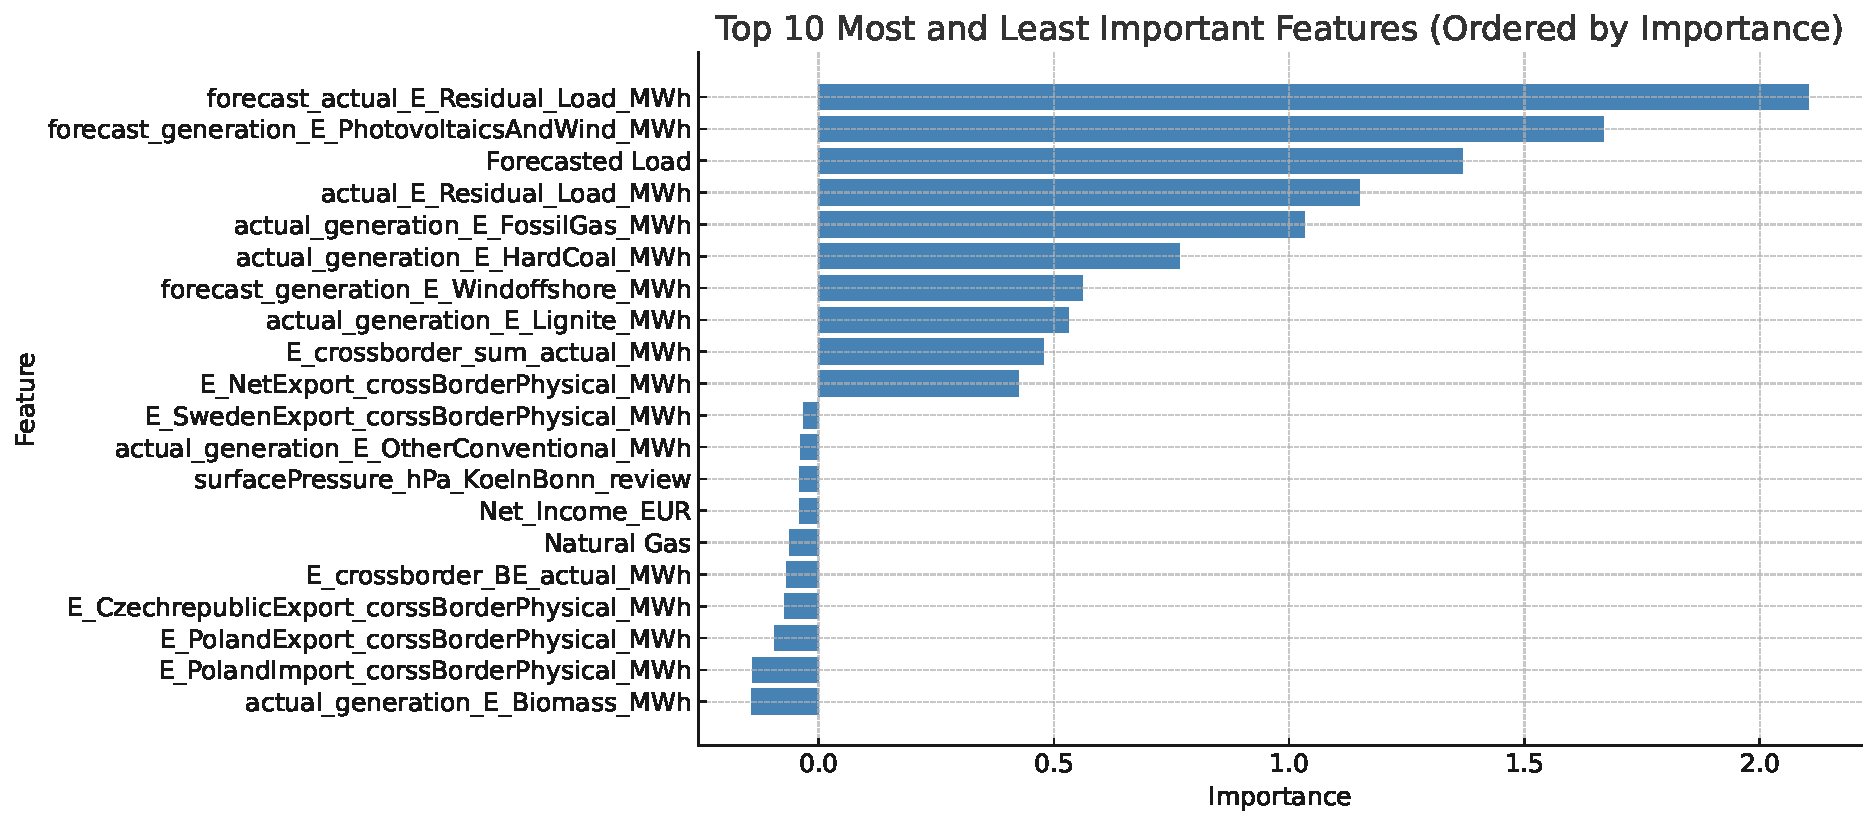
\includegraphics[keepaspectratio]{src/feature_importance_plot.pdf}}
\caption{Ten most and least important feature importances found by AG
when considering all covariates as known ahead of time}
\end{figure}

    However, as most of our data is unknown for the future, this approach
can not be utilized out of the box. Hence, we explored an approach to
provide future values regardless, simply by forecasting them. For this,
the best model trained on the assumption that all features are known
covariates was used. However, forecasts were provided for each feature
instead of the true future values during evaluation. This is depicted
below. To calculate those sub-forecasts, we used a pretrained Chronos
model. As shown in previous experiments (presented above), the
pretrained-only Chronos model already performs well. Additionaly, using
Chronos allows us to use the same model via weight sharing for
forecasting each feature, this saves memory and speeds up the prediction
process.

\begin{figure}
\centering
{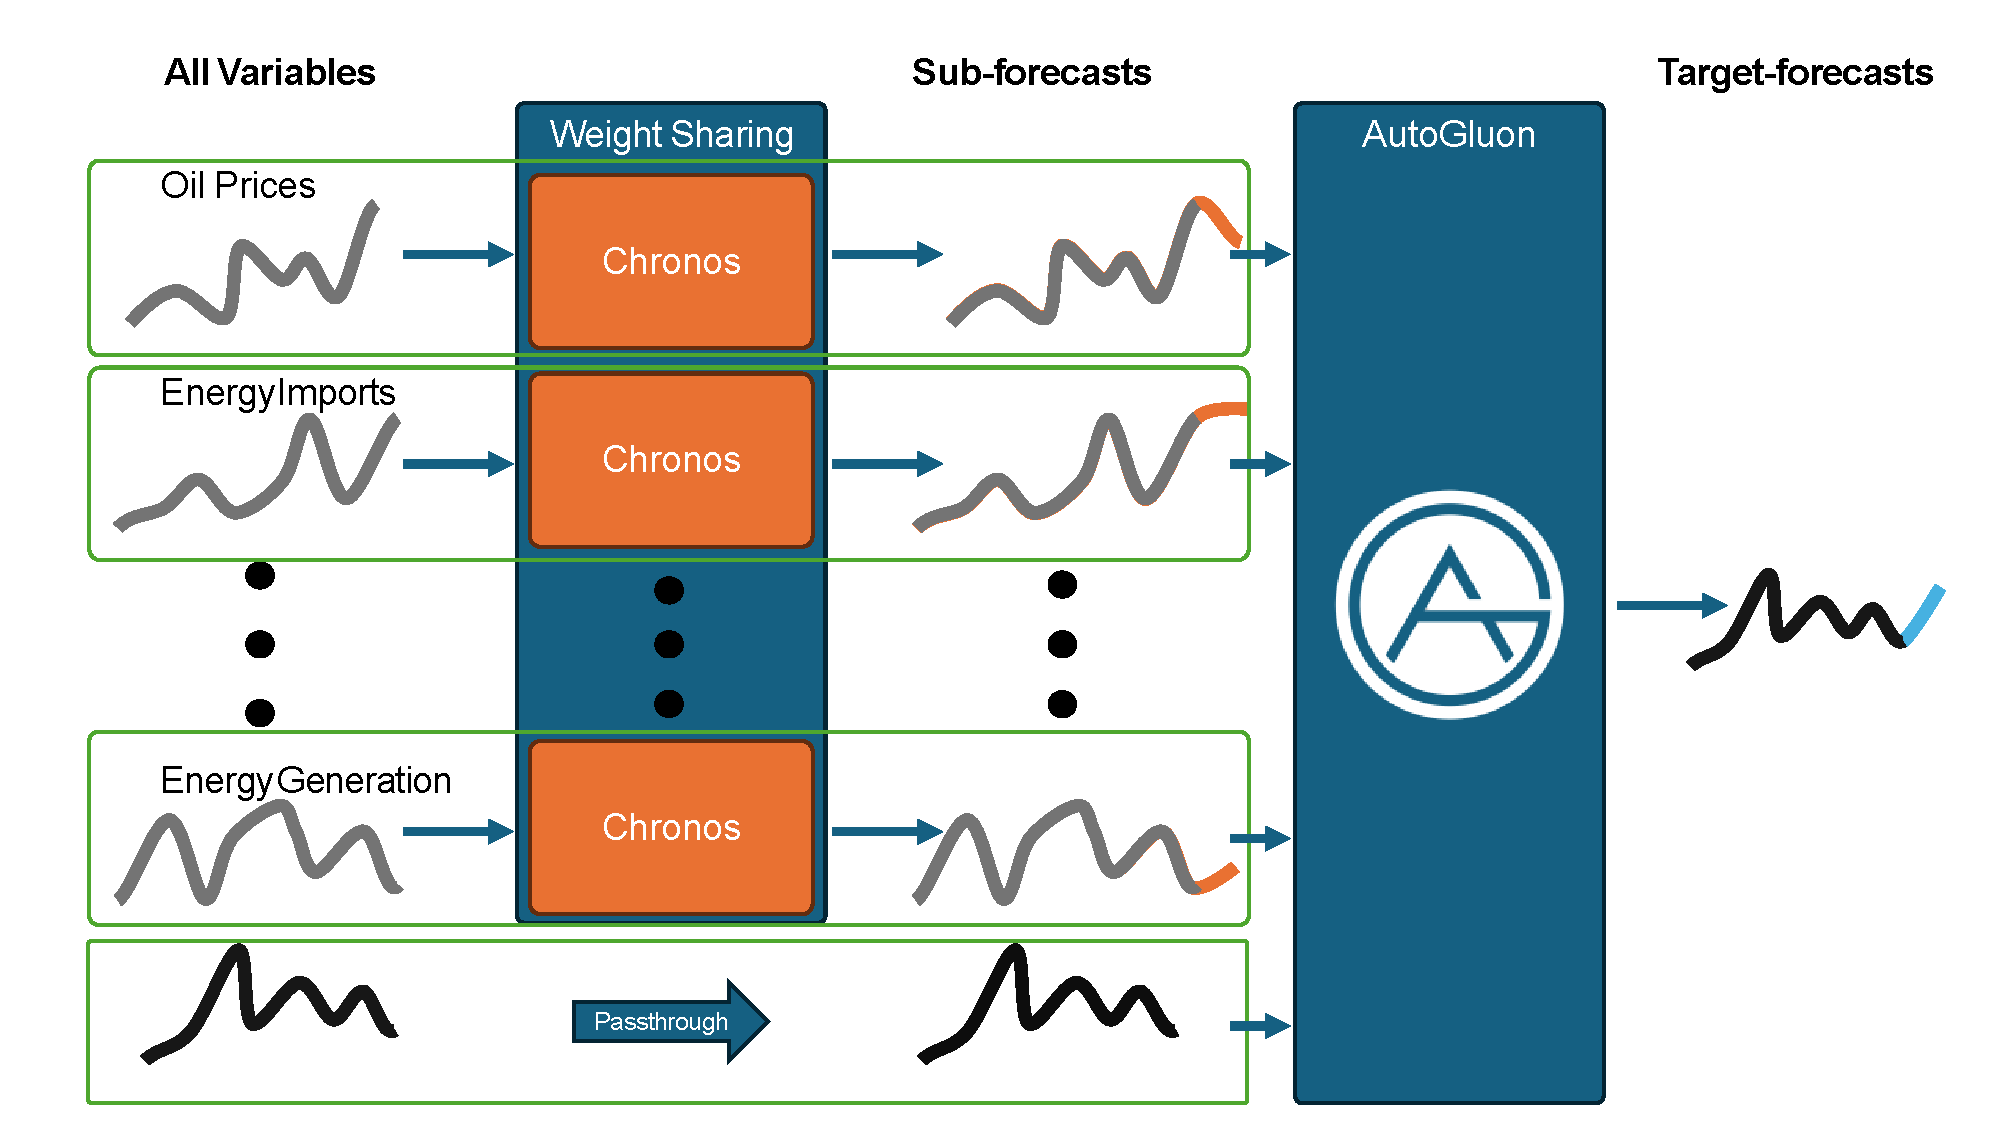
\includegraphics[keepaspectratio]{src/AG-Ensemble2.pdf}}
\caption{AG-Ensemble}
\end{figure}

With this approach, an MAE of 24.08 was achieved. Unfortunately, this
result is significantly worse than the prediction without known
covariates. This discrepancy is likely the result of errors in the
sub-forecasts that propagate to the final forecast conducted by AG. The
resulting predictions for the test period are shown in the figure below.
There, they are compared with the actual values and the previous best
model, AG High Quality Less without Known Covariates.

    \begin{tcolorbox}[breakable, size=fbox, boxrule=1pt, pad at break*=1mm,colback=cellbackground, colframe=cellborder]
\prompt{In}{incolor}{1}{\boxspacing}
\begin{small}
\begin{Verbatim}[commandchars=\\\{\}]
\PY{k+kn}{import}\PY{+w}{ }\PY{n+nn}{pandas}\PY{+w}{ }\PY{k}{as}\PY{+w}{ }\PY{n+nn}{pd}
\PY{k+kn}{import}\PY{+w}{ }\PY{n+nn}{matplotlib}\PY{n+nn}{.}\PY{n+nn}{pyplot}\PY{+w}{ }\PY{k}{as}\PY{+w}{ }\PY{n+nn}{plt}

\PY{n}{df1} \PY{o}{=} \PY{n}{pd}\PY{o}{.}\PY{n}{read\PYZus{}csv}\PY{p}{(}\PY{l+s+s1}{\PYZsq{}}\PY{l+s+s1}{./temp/comparison\PYZhy{}forecastet\PYZhy{}known\PYZhy{}ag.csv}\PY{l+s+s1}{\PYZsq{}}\PY{p}{,} \PY{n}{parse\PYZus{}dates}\PY{o}{=}\PY{p}{[}\PY{l+s+s1}{\PYZsq{}}\PY{l+s+s1}{timestamp}\PY{l+s+s1}{\PYZsq{}}\PY{p}{]}\PY{p}{)}
\PY{n}{df2} \PY{o}{=} \PY{n}{pd}\PY{o}{.}\PY{n}{read\PYZus{}csv}\PY{p}{(}\PY{l+s+s1}{\PYZsq{}}\PY{l+s+s1}{./temp/comparison\PYZhy{}ag.csv}\PY{l+s+s1}{\PYZsq{}}\PY{p}{,} \PY{n}{parse\PYZus{}dates}\PY{o}{=}\PY{p}{[}\PY{l+s+s1}{\PYZsq{}}\PY{l+s+s1}{timestamp}\PY{l+s+s1}{\PYZsq{}}\PY{p}{]}\PY{p}{)}
\PY{n}{df1} \PY{o}{=} \PY{n}{df1}\PY{p}{[}\PY{p}{(}\PY{n}{df1}\PY{p}{[}\PY{l+s+s1}{\PYZsq{}}\PY{l+s+s1}{timestamp}\PY{l+s+s1}{\PYZsq{}}\PY{p}{]}\PY{o}{.}\PY{n}{dt}\PY{o}{.}\PY{n}{month} \PY{o}{==} \PY{l+m+mi}{10}\PY{p}{)}\PY{p}{]}
\PY{n}{df2} \PY{o}{=} \PY{n}{df2}\PY{p}{[}\PY{p}{(}\PY{n}{df2}\PY{p}{[}\PY{l+s+s1}{\PYZsq{}}\PY{l+s+s1}{timestamp}\PY{l+s+s1}{\PYZsq{}}\PY{p}{]}\PY{o}{.}\PY{n}{dt}\PY{o}{.}\PY{n}{month} \PY{o}{==} \PY{l+m+mi}{10}\PY{p}{)}\PY{p}{]}

\PY{n}{plt}\PY{o}{.}\PY{n}{figure}\PY{p}{(}\PY{n}{figsize}\PY{o}{=}\PY{p}{(}\PY{l+m+mi}{12}\PY{p}{,} \PY{l+m+mi}{6}\PY{p}{)}\PY{p}{)}
\PY{n}{plt}\PY{o}{.}\PY{n}{plot}\PY{p}{(}\PY{n}{df1}\PY{p}{[}\PY{l+s+s1}{\PYZsq{}}\PY{l+s+s1}{timestamp}\PY{l+s+s1}{\PYZsq{}}\PY{p}{]}\PY{p}{,} \PY{n}{df1}\PY{p}{[}\PY{l+s+s1}{\PYZsq{}}\PY{l+s+s1}{actual\PYZus{}price}\PY{l+s+s1}{\PYZsq{}}\PY{p}{]}\PY{p}{,} \PY{n}{label}\PY{o}{=}\PY{l+s+s1}{\PYZsq{}}\PY{l+s+s1}{Actual Day Ahead Price}\PY{l+s+s1}{\PYZsq{}}\PY{p}{,} \PY{n}{marker}\PY{o}{=}\PY{l+s+s1}{\PYZsq{}}\PY{l+s+s1}{o}\PY{l+s+s1}{\PYZsq{}}\PY{p}{)}
\PY{n}{plt}\PY{o}{.}\PY{n}{plot}\PY{p}{(}\PY{n}{df1}\PY{p}{[}\PY{l+s+s1}{\PYZsq{}}\PY{l+s+s1}{timestamp}\PY{l+s+s1}{\PYZsq{}}\PY{p}{]}\PY{p}{,} \PY{n}{df1}\PY{p}{[}\PY{l+s+s1}{\PYZsq{}}\PY{l+s+s1}{mean}\PY{l+s+s1}{\PYZsq{}}\PY{p}{]}\PY{p}{,} \PY{n}{label}\PY{o}{=}\PY{l+s+s1}{\PYZsq{}}\PY{l+s+s1}{Predicted Day Ahead Price with predicted known\PYZhy{}covariables}\PY{l+s+s1}{\PYZsq{}}\PY{p}{,} \PY{n}{marker}\PY{o}{=}\PY{l+s+s1}{\PYZsq{}}\PY{l+s+s1}{x}\PY{l+s+s1}{\PYZsq{}}\PY{p}{)}
\PY{n}{plt}\PY{o}{.}\PY{n}{plot}\PY{p}{(}\PY{n}{df2}\PY{p}{[}\PY{l+s+s1}{\PYZsq{}}\PY{l+s+s1}{timestamp}\PY{l+s+s1}{\PYZsq{}}\PY{p}{]}\PY{p}{,} \PY{n}{df2}\PY{p}{[}\PY{l+s+s1}{\PYZsq{}}\PY{l+s+s1}{predicted}\PY{l+s+s1}{\PYZsq{}}\PY{p}{]}\PY{p}{,} \PY{n}{label}\PY{o}{=}\PY{l+s+s1}{\PYZsq{}}\PY{l+s+s1}{Predicted Day Ahead Price without predicted known\PYZhy{}covariables}\PY{l+s+s1}{\PYZsq{}}\PY{p}{,} \PY{n}{linestyle}\PY{o}{=}\PY{l+s+s1}{\PYZsq{}}\PY{l+s+s1}{\PYZhy{}\PYZhy{}}\PY{l+s+s1}{\PYZsq{}}\PY{p}{)}


\PY{n}{plt}\PY{o}{.}\PY{n}{title}\PY{p}{(}\PY{l+s+s1}{\PYZsq{}}\PY{l+s+s1}{Day Ahead Price Comparison}\PY{l+s+s1}{\PYZsq{}}\PY{p}{)}
\PY{n}{plt}\PY{o}{.}\PY{n}{xlabel}\PY{p}{(}\PY{l+s+s1}{\PYZsq{}}\PY{l+s+s1}{Timestamp}\PY{l+s+s1}{\PYZsq{}}\PY{p}{)}
\PY{n}{plt}\PY{o}{.}\PY{n}{ylabel}\PY{p}{(}\PY{l+s+s1}{\PYZsq{}}\PY{l+s+s1}{Day Ahead Price}\PY{l+s+s1}{\PYZsq{}}\PY{p}{)}
\PY{n}{plt}\PY{o}{.}\PY{n}{xticks}\PY{p}{(}\PY{n}{rotation}\PY{o}{=}\PY{l+m+mi}{45}\PY{p}{)}
\PY{n}{plt}\PY{o}{.}\PY{n}{legend}\PY{p}{(}\PY{p}{)}
\PY{n}{plt}\PY{o}{.}\PY{n}{tight\PYZus{}layout}\PY{p}{(}\PY{p}{)}


\PY{n}{plt}\PY{o}{.}\PY{n}{show}\PY{p}{(}\PY{p}{)}
\end{Verbatim}
\end{small}
\end{tcolorbox}

    \begin{center}
    \adjustimage{max size={0.9\linewidth}{0.9\paperheight}}{output_168_0.png}
    \end{center}
    { \hspace*{\fill} \\}
    
    

    \subsection{Conclusion}\label{conclusion}

    With the rapid expansion of renewable energy sources, day-ahead
electricity prices have become increasingly volatile. The availability
of solar and wind power plays a crucial role in determining these
prices, leading to significant fluctuations.

When renewable energy production is high, electricity prices can
plummet, sometimes even falling below zero. This phenomenon has become
more frequent in recent years: in 2022, there were 69 hours of negative
pricing, but this number surged to 301 hours in 2023 and further
increased to 459 hours in 2024.

Conversely, during periods of low renewable output---such as in winter
when sunlight and wind are scarce---electricity prices can soar to
extreme levels. This was evident in early November and mid-December
2024, when day-ahead prices exceeded 800 euros per megawatt-hour (MWh).

These extreme price swings present a fundamental for the presented
models. Since such rare events occur infrequently, they are
underrepresented in historical data. As a result, even advanced models
struggle to anticipate these anomalies with precision. The absence of
comparable training data means that models can recognize general trends
but remain unreliable when predicting rare, high-impact events in energy
markets.

    In this chapter, we investigated three different approaches to enhance
our models and improve forecasting. We investigated Long Short-Term
Memory networks (LSTMs) as a Recurrent Neural Network-based approach and
refined them further by extending to an encoder-decoder LSTM,
incorporating an attention mechanism, and leveraging multivariate data.
Our results showed that the Encoder-Decoder-Attention LSTM delivered the
best performance.

We then use Chronos as a transformer-based approach and improved it
through fine-tuning. Additionally, we investigated different fine-tuning
configurations and demonstrated that the large model, trained on a
substantial dataset with 1,000 training steps, performed the best.

Temporal Fusion Transformers (TFT), a second transformer-based approach
was used which is capable of handling multivariate data. We trained the
model on various features and examined how it responds to extreme
scenarios.

We utilize AutoGluon, an AutoML framework, to combine the advantages of
multiple models. To further enhance its performance, we conducted
experiments incorporating news embeddings and intra-day price forecasts.

    \section{Predictive Modeling}\label{predictive-modeling}

    In this section, we compare our best-performing models introduced in
\hyperref[visualization-and-story-telling]{Section 5}. The best model
will be used to perform the final forecast to predict the day-ahead
energy prices for the 2025-02-18.

    \subsection{Final Benchmark}\label{final-benchmark}

    We compare our models against each other and a baseline model that
predicts day-ahead prices using a simple 1-day shift. To evaluate their
performance on the test set, we use Mean Absolute Error (MAE) and Root
Mean Squared Error (RMSE). The test set consists of day-ahead prices
from June 1, 2024, to November 30, 2024.

    \begin{tcolorbox}[breakable, size=fbox, boxrule=1pt, pad at break*=1mm,colback=cellbackground, colframe=cellborder]
\prompt{In}{incolor}{8}{\boxspacing}
\begin{small}
\begin{Verbatim}[commandchars=\\\{\}]
\PY{c+c1}{\PYZsh{} ! set path your path to the \PYZsq{}temp\PYZsq{} dir}
\PY{n}{report\PYZus{}temp\PYZus{}dir} \PY{o}{=} \PY{l+s+s1}{\PYZsq{}}\PY{l+s+se}{\PYZbs{}\PYZbs{}}\PY{l+s+s1}{temp}\PY{l+s+s1}{\PYZsq{}}

\PY{n}{lstm\PYZus{}res} \PY{o}{=} \PY{n}{pd}\PY{o}{.}\PY{n}{read\PYZus{}csv}\PY{p}{(}\PY{n}{report\PYZus{}temp\PYZus{}dir} \PY{o}{+} \PY{l+s+s1}{\PYZsq{}}\PY{l+s+se}{\PYZbs{}\PYZbs{}}\PY{l+s+s1}{lstm\PYZus{}final\PYZus{}benchmark\PYZus{}test\PYZus{}results\PYZus{}48h.csv}\PY{l+s+s1}{\PYZsq{}}\PY{p}{,}
                       \PY{n}{index\PYZus{}col}\PY{o}{=}\PY{l+m+mi}{0}\PY{p}{)}\PY{p}{[}\PY{p}{[}\PY{l+s+s1}{\PYZsq{}}\PY{l+s+s1}{day\PYZus{}ahead\PYZus{}price\PYZus{}predicted}\PY{l+s+s1}{\PYZsq{}}\PY{p}{]}\PY{p}{]}
\PY{n}{chronos\PYZus{}large\PYZus{}finetuned\PYZus{}res} \PY{o}{=} \PY{n}{pd}\PY{o}{.}\PY{n}{read\PYZus{}csv}\PY{p}{(}\PY{n}{report\PYZus{}temp\PYZus{}dir} \PY{o}{+} \PY{l+s+s1}{\PYZsq{}}\PY{l+s+se}{\PYZbs{}\PYZbs{}}\PY{l+s+s1}{chronos\PYZus{}large\PYZus{}finetuned\PYZus{}final\PYZus{}benchmark\PYZus{}results.csv}\PY{l+s+s1}{\PYZsq{}}\PY{p}{,}
                                          \PY{n}{index\PYZus{}col}\PY{o}{=}\PY{l+m+mi}{0}\PY{p}{)}
\PY{n}{chronos\PYZus{}large\PYZus{}pretrained\PYZus{}res} \PY{o}{=} \PY{n}{pd}\PY{o}{.}\PY{n}{read\PYZus{}csv}\PY{p}{(}
    \PY{n}{report\PYZus{}temp\PYZus{}dir} \PY{o}{+} \PY{l+s+s1}{\PYZsq{}}\PY{l+s+se}{\PYZbs{}\PYZbs{}}\PY{l+s+s1}{chronos\PYZus{}large\PYZus{}pretrained\PYZus{}final\PYZus{}benchmark\PYZus{}results.csv}\PY{l+s+s1}{\PYZsq{}}\PY{p}{,} \PY{n}{index\PYZus{}col}\PY{o}{=}\PY{l+m+mi}{0}\PY{p}{)}
\PY{n}{chronos\PYZus{}tiny\PYZus{}finetuned\PYZus{}res} \PY{o}{=} \PY{n}{pd}\PY{o}{.}\PY{n}{read\PYZus{}csv}\PY{p}{(}\PY{n}{report\PYZus{}temp\PYZus{}dir} \PY{o}{+} \PY{l+s+s1}{\PYZsq{}}\PY{l+s+se}{\PYZbs{}\PYZbs{}}\PY{l+s+s1}{chronos\PYZus{}tiny\PYZus{}finetuned\PYZus{}final\PYZus{}benchmark\PYZus{}resuts.csv}\PY{l+s+s1}{\PYZsq{}}\PY{p}{,}
                                         \PY{n}{index\PYZus{}col}\PY{o}{=}\PY{l+m+mi}{0}\PY{p}{)}
\PY{n}{chronos\PYZus{}tiny\PYZus{}pretrained\PYZus{}res} \PY{o}{=} \PY{n}{pd}\PY{o}{.}\PY{n}{read\PYZus{}csv}\PY{p}{(}\PY{n}{report\PYZus{}temp\PYZus{}dir} \PY{o}{+} \PY{l+s+s1}{\PYZsq{}}\PY{l+s+se}{\PYZbs{}\PYZbs{}}\PY{l+s+s1}{chronos\PYZus{}tiny\PYZus{}pretrained\PYZus{}final\PYZus{}benchmark\PYZus{}results.csv}\PY{l+s+s1}{\PYZsq{}}\PY{p}{,}
                                          \PY{n}{index\PYZus{}col}\PY{o}{=}\PY{l+m+mi}{0}\PY{p}{)}
\PY{n}{autogluon\PYZus{}res} \PY{o}{=} \PY{n}{pd}\PY{o}{.}\PY{n}{read\PYZus{}csv}\PY{p}{(}\PY{n}{report\PYZus{}temp\PYZus{}dir} \PY{o}{+} \PY{l+s+s1}{\PYZsq{}}\PY{l+s+se}{\PYZbs{}\PYZbs{}}\PY{l+s+s1}{Autogluon\PYZus{}high\PYZus{}quality\PYZus{}less\PYZus{}without\PYZus{}known\PYZus{}covariables.csv}\PY{l+s+s1}{\PYZsq{}}\PY{p}{,}
                            \PY{n}{index\PYZus{}col}\PY{o}{=}\PY{l+m+mi}{0}\PY{p}{)}\PY{p}{[}\PY{p}{[}\PY{l+s+s1}{\PYZsq{}}\PY{l+s+s1}{predicted}\PY{l+s+s1}{\PYZsq{}}\PY{p}{]}\PY{p}{]}
\PY{n}{tft\PYZus{}res} \PY{o}{=} \PY{n}{pd}\PY{o}{.}\PY{n}{read\PYZus{}csv}\PY{p}{(}\PY{n}{report\PYZus{}temp\PYZus{}dir} \PY{o}{+} \PY{l+s+s1}{\PYZsq{}}\PY{l+s+se}{\PYZbs{}\PYZbs{}}\PY{l+s+s1}{tft\PYZus{}final\PYZus{}benchmark\PYZus{}results.csv}\PY{l+s+s1}{\PYZsq{}}\PY{p}{,} \PY{n}{index\PYZus{}col}\PY{o}{=}\PY{l+m+mi}{0}\PY{p}{)}
\PY{n}{previous\PYZus{}day\PYZus{}baseline} \PY{o}{=} \PY{n}{pd}\PY{o}{.}\PY{n}{read\PYZus{}csv}\PY{p}{(}\PY{n}{report\PYZus{}temp\PYZus{}dir} \PY{o}{+} \PY{l+s+s1}{\PYZsq{}}\PY{l+s+se}{\PYZbs{}\PYZbs{}}\PY{l+s+s1}{small\PYZus{}subset\PYZus{}lstm\PYZus{}cleaned.csv}\PY{l+s+s1}{\PYZsq{}}\PY{p}{)}\PY{p}{[}
    \PY{p}{[}\PY{l+s+s1}{\PYZsq{}}\PY{l+s+s1}{Date}\PY{l+s+s1}{\PYZsq{}}\PY{p}{,} \PY{l+s+s1}{\PYZsq{}}\PY{l+s+s1}{prev\PYZus{}range\PYZus{}prices}\PY{l+s+s1}{\PYZsq{}}\PY{p}{]}\PY{p}{]}\PY{o}{.}\PY{n}{set\PYZus{}index}\PY{p}{(}\PY{l+s+s1}{\PYZsq{}}\PY{l+s+s1}{Date}\PY{l+s+s1}{\PYZsq{}}\PY{p}{)}
\PY{n}{previous\PYZus{}day\PYZus{}baseline}\PY{o}{.}\PY{n}{index}\PY{o}{.}\PY{n}{names} \PY{o}{=} \PY{p}{[}\PY{l+s+s1}{\PYZsq{}}\PY{l+s+s1}{timestamp}\PY{l+s+s1}{\PYZsq{}}\PY{p}{]}

\PY{n}{actual\PYZus{}day\PYZus{}ahead\PYZus{}prices} \PY{o}{=} \PY{n}{pd}\PY{o}{.}\PY{n}{read\PYZus{}csv}\PY{p}{(}\PY{n}{report\PYZus{}temp\PYZus{}dir} \PY{o}{+} \PY{l+s+s1}{\PYZsq{}}\PY{l+s+se}{\PYZbs{}\PYZbs{}}\PY{l+s+s1}{small\PYZus{}subset\PYZus{}lstm\PYZus{}cleaned.csv}\PY{l+s+s1}{\PYZsq{}}\PY{p}{)}\PY{p}{[}
    \PY{p}{[}\PY{l+s+s1}{\PYZsq{}}\PY{l+s+s1}{Date}\PY{l+s+s1}{\PYZsq{}}\PY{p}{,} \PY{l+s+s1}{\PYZsq{}}\PY{l+s+s1}{day\PYZus{}ahead\PYZus{}prices}\PY{l+s+s1}{\PYZsq{}}\PY{p}{]}\PY{p}{]}\PY{o}{.}\PY{n}{set\PYZus{}index}\PY{p}{(}\PY{l+s+s1}{\PYZsq{}}\PY{l+s+s1}{Date}\PY{l+s+s1}{\PYZsq{}}\PY{p}{)}
\PY{n}{actual\PYZus{}day\PYZus{}ahead\PYZus{}prices}\PY{o}{.}\PY{n}{index}\PY{o}{.}\PY{n}{names} \PY{o}{=} \PY{p}{[}\PY{l+s+s1}{\PYZsq{}}\PY{l+s+s1}{timestamp}\PY{l+s+s1}{\PYZsq{}}\PY{p}{]}
\end{Verbatim}
\end{small}
\end{tcolorbox}

    \begin{tcolorbox}[breakable, size=fbox, boxrule=1pt, pad at break*=1mm,colback=cellbackground, colframe=cellborder]
\prompt{In}{incolor}{13}{\boxspacing}
\begin{small}
\begin{Verbatim}[commandchars=\\\{\}]
\PY{n}{BenchMaker} \PY{o}{=} \PY{n}{BenchmarkMaker}\PY{p}{(}\PY{n}{export\PYZus{}dir}\PY{o}{=}\PY{l+s+s1}{\PYZsq{}}\PY{l+s+s1}{results\PYZus{}from\PYZus{}report}\PY{l+s+s1}{\PYZsq{}}\PY{p}{)}
\PY{n}{BenchMaker}\PY{o}{.}\PY{n}{load\PYZus{}dataframes}\PY{p}{(}\PY{n}{predictions}\PY{o}{=}\PY{p}{\PYZob{}}\PY{l+s+s1}{\PYZsq{}}\PY{l+s+s1}{Baseline t\PYZhy{}24h}\PY{l+s+s1}{\PYZsq{}}\PY{p}{:} \PY{n}{previous\PYZus{}day\PYZus{}baseline}\PY{p}{,}
                                        \PY{l+s+s1}{\PYZsq{}}\PY{l+s+s1}{TFT}\PY{l+s+s1}{\PYZsq{}}\PY{p}{:} \PY{n}{tft\PYZus{}res}\PY{p}{,}
                                        \PY{l+s+s1}{\PYZsq{}}\PY{l+s+s1}{EncDecAtt LSTM}\PY{l+s+s1}{\PYZsq{}}\PY{p}{:} \PY{n}{lstm\PYZus{}res}\PY{p}{,}
                                        \PY{l+s+s1}{\PYZsq{}}\PY{l+s+s1}{AutoGluon}\PY{l+s+s1}{\PYZsq{}}\PY{p}{:} \PY{n}{autogluon\PYZus{}res}\PY{p}{,}
                                        \PY{l+s+s1}{\PYZsq{}}\PY{l+s+s1}{Chronos Finetuned Large}\PY{l+s+s1}{\PYZsq{}}\PY{p}{:} \PY{n}{chronos\PYZus{}large\PYZus{}finetuned\PYZus{}res}\PY{p}{\PYZcb{}}\PY{p}{,}
                           \PY{n}{prices}\PY{o}{=}\PY{n}{actual\PYZus{}day\PYZus{}ahead\PYZus{}prices}\PY{p}{)}
\PY{n}{BenchMaker}\PY{o}{.}\PY{n}{calc\PYZus{}errors}\PY{p}{(}\PY{p}{)}

\PY{n}{BenchMaker}\PY{o}{.}\PY{n}{plot\PYZus{}compare\PYZus{}mae}\PY{p}{(}\PY{p}{)}
\PY{n}{BenchMaker}\PY{o}{.}\PY{n}{plot\PYZus{}compare\PYZus{}rmse}\PY{p}{(}\PY{p}{)}
\PY{n}{BenchMaker}\PY{o}{.}\PY{n}{plot\PYZus{}compare\PYZus{}predictions\PYZus{}hourly}\PY{p}{(}\PY{n}{start\PYZus{}date}\PY{o}{=}\PY{n}{pd}\PY{o}{.}\PY{n}{Timestamp}\PY{p}{(}\PY{l+s+s1}{\PYZsq{}}\PY{l+s+s1}{2024\PYZhy{}06\PYZhy{}01 00:00:00}\PY{l+s+s1}{\PYZsq{}}\PY{p}{)}\PY{p}{,}
                                           \PY{n}{end\PYZus{}date}\PY{o}{=}\PY{n}{pd}\PY{o}{.}\PY{n}{Timestamp}\PY{p}{(}\PY{l+s+s1}{\PYZsq{}}\PY{l+s+s1}{2024\PYZhy{}06\PYZhy{}07 23:00:00}\PY{l+s+s1}{\PYZsq{}}\PY{p}{)}\PY{p}{)}
\end{Verbatim}
\end{small}
\end{tcolorbox}

    \begin{center}
    \adjustimage{max size={0.9\linewidth}{0.9\paperheight}}{output_178_0.png}
    \end{center}
    { \hspace*{\fill} \\}
    
    \begin{center}
    \adjustimage{max size={0.9\linewidth}{0.9\paperheight}}{output_178_1.png}
    \end{center}
    { \hspace*{\fill} \\}
    
    \begin{center}
    \adjustimage{max size={0.9\linewidth}{0.9\paperheight}}{output_178_2.png}
    \end{center}
    { \hspace*{\fill} \\}
    
    All models outperform the baseline, with the two best-performing ones
being the fine-tuned Chronos-T5 (Large) model and the AutoGluon
framework. AutoGluon achieved better results in terms of RMSE, while
Chronos-T5 performed better for MAE. The LSTM and TFT approaches also
showed promising results.

Nonetheless, Chronos and AutoGluon perform fairly similarly. This is
likely because AutoGluon often relies on Chronos models under the hood
to make its forecasts. For this it performs it own finetuning and
ensembles Chronos with other established Forecasting models.
Additionally, we find that AutoGluon uses a newer and improved version
of Chronos compared to ours that was published in the recent weeks.

However, our Hyperparameter optimized finetuning of Chronos seems to
have improved its accuraccy enough to still be very competitive with
this much more complex approach employed by AutoGluon.

    \subsection{Final Forecast}\label{final-forecast}

    \begin{tcolorbox}[breakable, size=fbox, boxrule=1pt, pad at break*=1mm,colback=cellbackground, colframe=cellborder]
\prompt{In}{incolor}{ }{\boxspacing}
\begin{small}
\begin{Verbatim}[commandchars=\\\{\}]
\PY{c+c1}{\PYZsh{} Load the data}
\PY{n}{file\PYZus{}path} \PY{o}{=} \PY{l+s+s1}{\PYZsq{}}\PY{l+s+s1}{merged\PYZus{}data/data\PYZus{}collection/day\PYZus{}ahead\PYZus{}prices.csv}\PY{l+s+s1}{\PYZsq{}}
\PY{n}{data} \PY{o}{=} \PY{n}{pd}\PY{o}{.}\PY{n}{read\PYZus{}csv}\PY{p}{(}\PY{n}{file\PYZus{}path}\PY{p}{)}

\PY{c+c1}{\PYZsh{} Convert timestamp column to datetime (ensure it\PYZsq{}s in UTC)}
\PY{n}{data}\PY{p}{[}\PY{l+s+s1}{\PYZsq{}}\PY{l+s+s1}{Date}\PY{l+s+s1}{\PYZsq{}}\PY{p}{]} \PY{o}{=} \PY{n}{pd}\PY{o}{.}\PY{n}{to\PYZus{}datetime}\PY{p}{(}\PY{n}{data}\PY{p}{[}\PY{l+s+s1}{\PYZsq{}}\PY{l+s+s1}{timestamp}\PY{l+s+s1}{\PYZsq{}}\PY{p}{]}\PY{p}{,} \PY{n}{utc}\PY{o}{=}\PY{k+kc}{True}\PY{p}{)}

\PY{c+c1}{\PYZsh{} Filter data to include only timestamps **before** the cutoff date}
\PY{c+c1}{\PYZsh{}data = data[data[\PYZsq{}Date\PYZsq{}] \PYZlt{}= cutoff\PYZus{}date\PYZus{}utc]}

\PY{c+c1}{\PYZsh{} Set the index to Date}
\PY{n}{data}\PY{o}{.}\PY{n}{set\PYZus{}index}\PY{p}{(}\PY{l+s+s1}{\PYZsq{}}\PY{l+s+s1}{Date}\PY{l+s+s1}{\PYZsq{}}\PY{p}{,} \PY{n}{inplace}\PY{o}{=}\PY{k+kc}{True}\PY{p}{)}

\PY{c+c1}{\PYZsh{} Load the model}
\PY{n}{finalmodeldir} \PY{o}{=} \PY{l+s+s2}{\PYZdq{}}\PY{l+s+s2}{juliushanusch/chronos\PYZhy{}large\PYZhy{}final\PYZhy{}fine\PYZhy{}tuned\PYZhy{}day\PYZhy{}ahead\PYZhy{}prices}\PY{l+s+s2}{\PYZdq{}}
\PY{n}{model\PYZus{}type} \PY{o}{=} \PY{l+s+s2}{\PYZdq{}}\PY{l+s+s2}{Chronos}\PY{l+s+s2}{\PYZdq{}}
\PY{n}{model\PYZus{}name} \PY{o}{=} \PY{n}{finalmodeldir}

\PY{n}{model} \PY{o}{=} \PY{n}{ChronosModel}\PY{p}{(}\PY{n}{model\PYZus{}name}\PY{o}{=}\PY{n}{model\PYZus{}name}\PY{p}{,} \PY{n}{model\PYZus{}type}\PY{o}{=}\PY{n}{model\PYZus{}type}\PY{p}{)}
\PY{n}{model}\PY{o}{.}\PY{n}{model} \PY{o}{=} \PY{n}{model}\PY{o}{.}\PY{n}{custom\PYZus{}load}\PY{p}{(}\PY{n}{finalmodeldir}\PY{p}{)}

\PY{c+c1}{\PYZsh{} Forecast based on the filtered dataset}
\PY{n}{finalForecastChronos} \PY{o}{=} \PY{n}{model}\PY{o}{.}\PY{n}{run\PYZus{}prediction}\PY{p}{(}\PY{n}{data}\PY{p}{)}

\PY{c+c1}{\PYZsh{} Convert forecast timestamps to Berlin time (CET/CEST)}
\PY{n}{finalForecastChronos}\PY{p}{[}\PY{l+s+s1}{\PYZsq{}}\PY{l+s+s1}{timestamp}\PY{l+s+s1}{\PYZsq{}}\PY{p}{]} \PY{o}{=} \PY{n}{pd}\PY{o}{.}\PY{n}{to\PYZus{}datetime}\PY{p}{(}\PY{n}{finalForecastChronos}\PY{p}{[}\PY{l+s+s1}{\PYZsq{}}\PY{l+s+s1}{timestamp}\PY{l+s+s1}{\PYZsq{}}\PY{p}{]}\PY{p}{,} \PY{n}{utc}\PY{o}{=}\PY{k+kc}{True}\PY{p}{)}
\PY{n}{finalForecastChronos}\PY{p}{[}\PY{l+s+s1}{\PYZsq{}}\PY{l+s+s1}{timestamp}\PY{l+s+s1}{\PYZsq{}}\PY{p}{]} \PY{o}{=} \PY{n}{finalForecastChronos}\PY{p}{[}\PY{l+s+s1}{\PYZsq{}}\PY{l+s+s1}{timestamp}\PY{l+s+s1}{\PYZsq{}}\PY{p}{]}\PY{o}{.}\PY{n}{dt}\PY{o}{.}\PY{n}{tz\PYZus{}convert}\PY{p}{(}\PY{l+s+s1}{\PYZsq{}}\PY{l+s+s1}{Europe/Berlin}\PY{l+s+s1}{\PYZsq{}}\PY{p}{)}
\end{Verbatim}
\end{small}
\end{tcolorbox}

    \begin{tcolorbox}[breakable, size=fbox, boxrule=1pt, pad at break*=1mm,colback=cellbackground, colframe=cellborder]
\prompt{In}{incolor}{13}{\boxspacing}
\begin{small}
\begin{Verbatim}[commandchars=\\\{\}]
\PY{k+kn}{import}\PY{+w}{ }\PY{n+nn}{pandas}\PY{+w}{ }\PY{k}{as}\PY{+w}{ }\PY{n+nn}{pd}
\PY{k+kn}{import}\PY{+w}{ }\PY{n+nn}{matplotlib}\PY{n+nn}{.}\PY{n+nn}{pyplot}\PY{+w}{ }\PY{k}{as}\PY{+w}{ }\PY{n+nn}{plt}

\PY{n}{file\PYZus{}path} \PY{o}{=} \PY{l+s+s2}{\PYZdq{}}\PY{l+s+s2}{finalForecastPlot.csv}\PY{l+s+s2}{\PYZdq{}}  
\PY{n}{df} \PY{o}{=} \PY{n}{pd}\PY{o}{.}\PY{n}{read\PYZus{}csv}\PY{p}{(}\PY{n}{file\PYZus{}path}\PY{p}{)}

\PY{n}{df}\PY{p}{[}\PY{l+s+s2}{\PYZdq{}}\PY{l+s+s2}{timestamp}\PY{l+s+s2}{\PYZdq{}}\PY{p}{]} \PY{o}{=} \PY{n}{pd}\PY{o}{.}\PY{n}{to\PYZus{}datetime}\PY{p}{(}\PY{n}{df}\PY{p}{[}\PY{l+s+s2}{\PYZdq{}}\PY{l+s+s2}{timestamp}\PY{l+s+s2}{\PYZdq{}}\PY{p}{]}\PY{p}{)}

\PY{c+c1}{\PYZsh{} Plot the values for Germany/Luxembourg}
\PY{n}{plt}\PY{o}{.}\PY{n}{figure}\PY{p}{(}\PY{n}{figsize}\PY{o}{=}\PY{p}{(}\PY{l+m+mi}{12}\PY{p}{,} \PY{l+m+mi}{6}\PY{p}{)}\PY{p}{)}
\PY{n}{plt}\PY{o}{.}\PY{n}{plot}\PY{p}{(}\PY{n}{df}\PY{p}{[}\PY{l+s+s2}{\PYZdq{}}\PY{l+s+s2}{timestamp}\PY{l+s+s2}{\PYZdq{}}\PY{p}{]}\PY{p}{,} \PY{n}{df}\PY{p}{[}\PY{l+s+s2}{\PYZdq{}}\PY{l+s+s2}{Germany/Luxembourg in \euro{}/MWh}\PY{l+s+s2}{\PYZdq{}}\PY{p}{]}\PY{p}{,} \PY{n}{label}\PY{o}{=}\PY{l+s+s2}{\PYZdq{}}\PY{l+s+s2}{Germany/Luxembourg in \euro{}/MWh predicted}\PY{l+s+s2}{\PYZdq{}}\PY{p}{,} \PY{n}{color}\PY{o}{=}\PY{l+s+s2}{\PYZdq{}}\PY{l+s+s2}{blue}\PY{l+s+s2}{\PYZdq{}}\PY{p}{)}
\PY{n}{plt}\PY{o}{.}\PY{n}{plot}\PY{p}{(}\PY{n}{df}\PY{p}{[}\PY{l+s+s2}{\PYZdq{}}\PY{l+s+s2}{timestamp}\PY{l+s+s2}{\PYZdq{}}\PY{p}{]}\PY{p}{,} \PY{n}{df}\PY{p}{[}\PY{l+s+s2}{\PYZdq{}}\PY{l+s+s2}{last year}\PY{l+s+s2}{\PYZdq{}}\PY{p}{]}\PY{p}{,} \PY{n}{label}\PY{o}{=}\PY{l+s+s2}{\PYZdq{}}\PY{l+s+s2}{Germany/Luxembourg in  \euro{}/MWh last year}\PY{l+s+s2}{\PYZdq{}}\PY{p}{,} \PY{n}{color}\PY{o}{=}\PY{l+s+s2}{\PYZdq{}}\PY{l+s+s2}{red}\PY{l+s+s2}{\PYZdq{}}\PY{p}{)}

\PY{n}{plt}\PY{o}{.}\PY{n}{ylim}\PY{p}{(}\PY{l+m+mi}{0}\PY{p}{,} \PY{l+m+mi}{250}\PY{p}{)}
\PY{n}{plt}\PY{o}{.}\PY{n}{xlabel}\PY{p}{(}\PY{l+s+s2}{\PYZdq{}}\PY{l+s+s2}{Hour}\PY{l+s+s2}{\PYZdq{}}\PY{p}{)}
\PY{n}{plt}\PY{o}{.}\PY{n}{ylabel}\PY{p}{(}\PY{l+s+s2}{\PYZdq{}}\PY{l+s+s2}{Price (\euro{}/MWh)}\PY{l+s+s2}{\PYZdq{}}\PY{p}{)}
\PY{n}{plt}\PY{o}{.}\PY{n}{title}\PY{p}{(}\PY{l+s+s2}{\PYZdq{}}\PY{l+s+s2}{Final Forecast And Last Year Prices}\PY{l+s+s2}{\PYZdq{}}\PY{p}{)}
\PY{n}{plt}\PY{o}{.}\PY{n}{legend}\PY{p}{(}\PY{p}{)}
\PY{n}{plt}\PY{o}{.}\PY{n}{xticks}\PY{p}{(}\PY{n}{rotation}\PY{o}{=}\PY{l+m+mi}{45}\PY{p}{)}
\PY{n}{plt}\PY{o}{.}\PY{n}{grid}\PY{p}{(}\PY{p}{)}
\PY{n}{plt}\PY{o}{.}\PY{n}{show}\PY{p}{(}\PY{p}{)}
\end{Verbatim}
\end{small}
\end{tcolorbox}

    \begin{center}
    \adjustimage{max size={0.9\linewidth}{0.9\paperheight}}{output_182_0.png}
    \end{center}
    { \hspace*{\fill} \\}
    
    \subsection{Conclusion}\label{conclusion}

We compared our best performing models and generated the final forecast.
Since Chronos showed the best results on the MAE we used this model for
the final forecast. We can see that the day-ahead energy price is
relatively high compared to the average and compared to the prices one
year ago which are presented in the plot above.

    \section{Summary \& Future Work}\label{summary-future-work}

    \subsection{Self-Organization in Academic
Projects}\label{self-organization-in-academic-projects}

Team Structure and Initial Organization: The BTW25 Data Science
challenge presented a unique opportunity to work in a large-scale
collaborative environment with twelve team members. To effectively
manage this substantial team size, we implemented a strategic division
into three specialized groups, each focusing on critical aspects of the
project:

\begin{itemize}
\tightlist
\item
  XAI and Data Preparation Group: Focused on explainable AI approaches
  and foundational data analysis
\item
  AutoGluon and Preprocessing Group: Concentrated on implementing
  solutions using AutoGluon and gathering data
\item
  Deep Learning Models Group: Dedicated to the development and
  application of complex neural network architectures
\end{itemize}

Challenges of Interdependent Workflows: One of the primary challenges we
faced was managing the interdependencies between these groups. Each
team's output served as essential input for others, creating a complex
web of dependencies. For example, the data fetching and preparation
team's work directly impacted both the XAIs ability to explore the data
and the deep learning team's capacity to develop their architectures.
This interconnected structure meant that delays or changes in one group
could create ripple effects throughout the entire project.

Cross-Team Communication and Coordination: To address these challenges,
we implemented an ``ambassador'' system. Members of the AutoGluon team
were designated as visitors to other groups, attending their meetings
and serving as communication bridges. This approach proved invaluable
for several reasons:

\begin{itemize}
\tightlist
\item
  Real-time awareness of progress and challenges across all teams
\item
  Immediate feedback on compatibility issues between different
  components
\item
  Rapid dissemination of important updates or changes
\item
  Prevention of duplicate efforts across groups
\end{itemize}

Standardization and Technical Integration: A crucial aspect of our
success was the implementation of strict technical standards:

Data Format Guidelines:

\begin{itemize}
\tightlist
\item
  Standardized CSV formats for time series data
\item
  Consistent datetime formatting across all datasets
\item
  Uniform naming conventions for features and target variables
\item
  Desired range of data
\item
  Clear separation of train/val/test splits
\end{itemize}

Model Wrapper Standardization:

\begin{itemize}
\tightlist
\item
  Common interface for all models regardless of underlying
  implementation
\item
  Standardized prediction output formats
\item
  Unified evaluation metrics and reporting structures
\end{itemize}

Effective Project Management Practices To maintain coherence across the
large team, we established several key management practices:

\begin{itemize}
\tightlist
\item
  Regular all-hands meetings for high-level coordination
\item
  Dedicated communication channels for each subgroup
\end{itemize}

Learning Outcomes and Best Practices This experience provided valuable
insights into managing large-scale ML projects:

\begin{itemize}
\tightlist
\item
  The importance of clear communication channels and protocols
\item
  The value of standardized interfaces between different components
\item
  The effectiveness of cross-team ambassadors in maintaining project
  coherence
\item
  The necessity of flexible yet structured organization in academic
  projects
\end{itemize}

Impact on Project Success These organizational strategies significantly
contributed to our project's success by:

\begin{itemize}
\tightlist
\item
  Minimizing integration issues between different components
\item
  Reducing redundant work across teams
\item
  Enabling rapid problem identification and resolution
\item
  Fostering knowledge sharing across specialization boundaries
\item
  Creating a cohesive final product despite the complexity of multiple
  approaches
\end{itemize}

The experience demonstrated that effective organization and
communication structures are as crucial to project success as technical
expertise, particularly in large-scale academic collaborations.

    \subsection{Future Work}\label{future-work}

\paragraph{Weather Improvements}\label{weather-improvements}

While the current weather implementation provides a solid foundation,
various measures could be implemented to further optimise the process:

\begin{itemize}
\item
  The installation of a greater number of weather stations would
  facilitate a more detailed and regionally differentiated depiction of
  weather conditions.
\item
  In addition, calculating an average at the country level has the
  potential to enhance the representativeness of the basis. This average
  could then be weighted with the population density and the regionally
  available capacity of the individual power plant types in order to
  better model local energy generation and demand.
\item
  Furthermore, the incorporation of extreme weather events, such as heat
  waves, cold snaps, and storms, is imperative for the analysis and
  forecasting of energy generation and demand. Including data on these
  events could facilitate more precise prediction of unexpected
  fluctuations in energy production and demand. The analysis of
  long-term weather patterns, including seasonal fluctuations and the
  effects of climate change, has the potential to significantly enhance
  forecasting accuracy.
\item
  Hyperparameter optimization for Chronos.
\end{itemize}

By expanding the analysed data set, weather implementation could be made
more precise and flexible, allowing it to respond better to the
requirements of a dynamic energy market.

    \paragraph{Advancing LSTM Models}\label{advancing-lstm-models}

Since the Encoder Decoder LSTM with attention has shown to be superior
to LSTM models without attention, it might lead to a further improved
forecasting accuracy to use an additional feature attention. This could
help the model to focus only on important features rather than weighting
each feature evenly. Also, LSTM models benefit strongly from a dataset
with substained features. Therefore, finding even more meaningful
features could support the model on learning correct forecasts. Further
optimizing the model on the combination of features, the model size and
other hyperparameters could possibly decrease the error of the final
forecast.

    \subsection{Summary}\label{summary}

This report describes the methodology used by the Dresden Database
Research Group to forecast day-ahead electricity prices as part of the
BTW 2025 Data Science Challenge. The focus was on the comparison and
optimisation of established time series forecasting methods to improve
forecasting accuracy. First, in-depth domain knowledge about energy
markets and electricity pricing was researched and analysed (\ref{gathering-domain-knowledge}~\nameref{gathering-domain-knowledge}). Several relevant data sources were then identified,
including financial, meteorological, and social factors that have a
significant influence on day-ahead prices. The data was analysed
iteratively, including an assessment of variance in SMARD data and an
evaluation of feature importance across different models. Additionally,
advanced data analysis techniques, including explainable AI, were
applied to gain deeper insights into the predictive models. Based on
this analysis, the individual we utilized various time series
forecasting models, including LSTM-based models, Chronos, Temporal
Fusion Transformer and AutoGluon (\ref{visualization-and-story-telling}~\nameref{visualization-and-story-telling}).
AutoGluon was enhanced through various tuning strategies, including
covariate forecasting, intraday calculations, and news embeddings to
improve performance. Chronos underwent fine-tuning to refine its
predictive capabilities , while TFT was implemented as a multivariate
transformer-based model. In a final benchmarking exercise, conducted
over a six-month period, the models were evaluated based on their
forecasting accuracy. The best-performing models from AutoGluon and
PyTorch were compared against a baseline (\ref{predictive-modeling}~\nameref{predictive-modeling}).
Chronos achieved the best MAE and was therefore selected for the
official forecast submission in the BTW 2025 Data Science Challenge.

    \subsection{Conclusion}\label{conclusion}

In conclusion, transformer models demonstrated superior performance
throughout the analysis, with several enhancements explored to improve
forecasting accuracy. Among the models, Chronos achieved the best
results when relying solely on the day-ahead price for predictions. We
fine-tuned Chronos using different configurations to optimize its
performance. As a fine-tuned model, the largest version of Chronos,
trained on a substantial dataset with 1,000 training steps, provided the
most accurate forecasts.

We also investigated Long Short-Term Memory networks as a recurrent
neural network-based approach, refining it further by extending to an
Encoder-Decoder LSTM with an attention mechanism and incorporating
multivariate data. The Encoder-Decoder-Attention LSTM delivered the best
performance among the recurrent models. Temporal Fusion Transformers,
another transformer-based approach capable of handling multivariate
data, were trained on various features, but performed worse than
Chronos. However, it showed the ability to respond to extreme scenarios,
providing additional insights into model behavior under different
conditions.

AutoGluon showed slightly lower performance as it used all available
data points, but it was enhanced by incorporating news embeddings and
intra-day price forecasts. While experimenting with known covariates for
all features in AG led to a performance boost, this approach was
ultimately not feasible due to the unavailability of most features in
advance. Overall, Chronos emerged as the most reliable model, with
transformer-based methods proving to be effective for day-ahead
electricity price forecasting.

    \newpage
\section{Bibliography}\label{bibliography}

\rowcolors{2}{white}{gray!25}
{\fontsize{8pt}{10pt}\selectfont\begin{longtable}[]{@{}
  >{\raggedright\arraybackslash}p{(\linewidth - 2\tabcolsep) * \real{0.1684}}
  >{\raggedright\arraybackslash}p{(\linewidth - 2\tabcolsep) * \real{0.8316}}@{}}
\toprule\noalign{}
\endhead
\bottomrule\noalign{}
\endlastfoot
{[}Ansari et al.~2024{]} & Abdul Fatir Ansari et al.~2024: Chronos:
Learning the Language of Time Series
https://doi.org/10.48550/arXiv.2403.07815 \\
{[}Bahdanau et al.~2014{]} & Bahdanau, D. (2014). Neural machine
translation by jointly learning to align and translate. arXiv preprint
arXiv:1409.0473. \\
{[}Bengio et al.~1993{]} & Y. Bengio, P. Frasconi and P. Simard, ``The
problem of learning long-term dependencies in recurrent networks,'' IEEE
International Conference on Neural Networks, San Francisco, CA, USA,
1993, pp.~1183-1188 vol.3, doi: 10.1109/ICNN.1993.298725. \\
{[}Bosch et al.~2023{]} & Bosch, S., Schlenker, F., Bohn, J., Kupies,
S., \& Schmidt, M. (2023). Deutschland--Pionierland der Energiewende. In
Energie-Weltatlas: Transformation des Energiesystems in globaler
Perspektive (pp.~81-91). Wiesbaden: Springer Fachmedien Wiesbaden \\
{[}Contreras et al.~2003{]} & Contreras, J., Espinola, R., Nogales, F.
J., \& Conejo, A. J. (2003). ARIMA models to predict next-day
electricity prices. IEEE transactions on power systems, 18(3),
1014-1020 \\
{[}Dumancic 2024{]} & Dumancic, M. (2024, March). Marktmacht in der
Stromwirtschaft: Mehr Wettbewerb durch Zukunftstechnologien?. In
Kartellrecht und Zukunftstechnologien (pp.~105-128). Nomos
Verlagsgesellschaft mbH \& Co.~KG. \\
{[}Hein et al.~2020{]} & Hein, F., \& Hermann, H. (2020).
Agorameter--Dokumentation. Agora Energiewende: Berlin, Germany. \\
{[}Hochreiter et al.~1997{]} & Hochreiter, Sepp \& Schmidhuber, Jürgen.
(1997). Long Short-Term Memory. Neural Computation. 9. 1735-1780.
10.1162/neco.1997.9.8.1735. \\
{[}Horáček 2010{]} & Horáček, P. (2010). Power balance control in
electrical grids. Seminary Textbooks, Faculty of Electrical
Engineering. \\
{[}Kandadi et al.~2025{]} & Kandadi, T., \& Shankarlingam, G. (2025).
DRAWBACKS OF LSTM ALGORITHM: A CASE STUDY. Available at SSRN 5080605. \\
{[}Lago et al.~2018{]} & Lago, J., De Ridder, F., \& De Schutter, B.
(2018). Forecasting spot electricity prices: Deep learning approaches
and empirical comparison of traditional algorithms. Applied Energy, 221,
386-405. \\
{[}Nestle et al.~2009{]} & Nestle, D., Ringelstein, J., \& Selzam, P.
(2009). Integration dezentraler und erneuerbarer Energien durch variable
Strompreise im liberalisierten Energiemarkt. uwf UmweltWirtschaftsForum,
17, 361-365. \\
{[}Niedermeier 2023{]} & Niedermeier, T. (2023). Auswertung der
Stromerzeugung in Deutschland von 2015--2022 und Abgleich mit den
Ausbauzielen des EEG 2023 (Doctoral dissertation, Hochschule für
angewandte Wissenschaften München). \\
{[}Nunes et al.~2008{]} & Nunes, C., Pacheco, A., \& Silva, T. (2008,
May). Statistical models to predict electricity prices. In 2008 5th
International Conference on the European Electricity Market (pp.~1-6).
IEEE. \\
{[}Ortner and Totschnig 2019{]} & Ortner, A., \& Totschnig, G. (2019).
The future relevance of electricity balancing markets in Europe-A 2030
case study. Energy Strategy Reviews, 24, 111-120. \\
{[}Parthipan et al.~2024{]} & Parthipan, R., Anand, M., Christensen, H.
M., Hosking, J. S., \& Wischik, D. J. (2024). Defining error
accumulation in ML atmospheric simulators. arXiv preprint
arXiv:2405.14714. \\
{[}Picasso et al.~2019{]} & Picasso et al., 2019: Technical analysis and
sentiment embeddings for market trend prediction \\
{[}Schumacher et al.~2015{]} & Schumacher, Ingrid, et al.~``Der
strommarkt und die strompreisbildung.'' Strategien zur Strombeschaffung
in Unternehmen: Energieeinkauf optimieren, Kosten senken (2015):
9-37. \\
{[}Schmidhuber et al.~2003{]} & Fakultät Informatik \& Bengio, Y. \&
Frasconi, Paolo \& Schmidhuber, Jürgen. (2003). Gradient Flow in
Recurrent Nets: the Difficulty of Learning Long-Term Dependencies. A
Field Guide to Dynamical Recurrent Neural Networks. \\
{[}Shur et al.~2023{]} & Shchur, O., Turkmen, C., Erickson, N., Shen,
H., Shirkov, A., Hu, T., Wang, T. (2023). AutoGluon-TimeSeries: AutoML
for Probabilistic Time Series Forecasting.
https://arxiv.org/abs/2308.05566 \\
{[}Steinmetz et al.~2022{]} & Steinmetz, H., Batzdorfer, V., Scherhag,
J., \& Bosnjak, M. (2022). The ZPID Lockdown Measures Dataset for
Germany {[}Data set{]}. PsychArchives.
https://doi.org/10.23668/PSYCHARCHIVES.6676 \\
{[}Sutskever et al.~2014{]} & Sutskever, I. (2014). Sequence to Sequence
Learning with Neural Networks. arXiv preprint arXiv:1409.3215. \\
{[}Tschora et al.~2022{]} & Tschora, L., Pierre, E., Plantevit, M., \&
Robardet, C. (2022). Electricity price forecasting on the day-ahead
market using machine learning. Applied Energy, 313, 118752. \\
{[}Vaswani et al.~2017{]} & Attention is all you need. Advances in
Neural Information Processing Systems. \\
{[}Yun Bai et al.~2024{]} & Yun Bai et al., 2024: News and Load: A
Quantitative Exploration of Natural Language Processing Applications for
Forecasting Day-Ahead Electricity System Demand \\
{[}Zhao et al.~2020{]} & Zhao, J., Huang, F., Lv, J., Duan, Y., Qin, Z.,
Li, G., \& Tian, G. (2020, November). Do RNN and LSTM have long memory?.
In International Conference on Machine Learning (pp.~11365-11375).
PMLR. \\
{[}AutoGluon Forecasting Model Zoo, 2025{]} & auto.gluon.ai, 16.02.2025,
URL:
https://auto.gluon.ai/dev/tutorials/timeseries/forecasting-model-zoo.html \\
{[}European Commission, EU ETS, 2024{]} & commission.europa.eu, European
Commission, 16.12.2024, URL:
https://climate.ec.europa.eu/eu-action/eu-emissions-trading-system-eu-ets\_en \\
{[}Finanztools, Inflationsraten Deutschland, 2025{]} & Finanz-tools.de,
Klaudia Will, 12.02.2025, URL:
https://www.finanz-tools.de/inflation/inflationsraten-deutschland \\
{[}Investing, Carbon Emissions Futures, 2024{]} & Investing.com, Fusion
Media Limited, 16.12.2024, URL:
https://www.investing.com/commodities/carbon-emissions-historical-data \\
{[}Netztransparenz, Index-Ausgleichspreis, 2024{]} & Netztransparenz.de,
50Hertz Transmission GmbH; Amprion GmbH; TenneT TSO GmbH; TransnetBW
GmbH, 16.12.2024, URL:
https://www.netztransparenz.de/de-de/Regelenergie/Ausgleichsenergiepreis/Index-Ausgleichsenergiepreis \\
{[}Smard, Großhandelspreise, 2024{]} & Smard.de, Bundesnetzagentur,
15.12.2024, URL: https://www.smard.de/page/home/wiki-article/446/562 \\
{[}Smard, Negative wholesale prices, 2025{]} & Smard.de,
Bundesnetzagentur, 13.02.2025, URL:
https://www.smard.de/page/en/wiki-article/5884/105426 \\
{[}Smard user guide, 2024{]} & Smard.de, Bundesnetzagentur, 15.12.2024,
URL:
\href{https://www.smard.de/resource/blob/205652/63fcff2c9813096fa2229d769da164ef/smard-user-guide-09-2021-data.pdf}{\color{black}https://www.smard.de/resource/blob/205652/63fcff2c9813096fa2229d769da164ef/}\hspace{0em}\href{https://www.smard.de/resource/blob/205652/63fcff2c9813096fa2229d769da164ef/smard-user-guide-09-2021-data.pdf}{\color{black}smard-user-guide-09-2021-data.pdf} \\
\end{longtable}}

    \vspace{15em}\subsection{Acknowledgement}\label{acknowledgement}

The authors gratefully acknowledge the computing time made available to
them on the high-performance computer at the NHR Center of TU Dresden.
This center is jointly supported by the Federal Ministry of Education
and Research and the state governments participating in the NHR
(www.nhr-verein.de/unsere-partner).

We sincerely thank our supervisors, Jimmy Pöhlmann, Claudio Hartmann,
and Wolfgang Lehner, for their guidance and support throughout the
semester and the development of this report. Their expertise, feedback,
and encouragement played an important role in shaping our work. We
appreciate their time and effort in mentoring us through this process.

    \newpage\appendix
\section{Appendix I: Smard Dataset
Columns}\label{appendix-i-smard-dataset-columns}

    \rowcolors{2}{white}{gray!25}
{\fontsize{8pt}{10pt}\selectfont\begin{longtable}[]{@{}
  >{\raggedright\arraybackslash}p{(\linewidth - 6\tabcolsep) * \real{0.25}}
  >{\raggedright\arraybackslash}p{(\linewidth - 6\tabcolsep) * \real{0.15}}
  >{\raggedright\arraybackslash}p{(\linewidth - 6\tabcolsep) * \real{0.2}}
  >{\raggedright\arraybackslash}p{(\linewidth - 6\tabcolsep) * \real{0.4}}@{}}
\toprule\noalign{}
\begin{minipage}[b]{\linewidth}\raggedright
Column Name
\end{minipage} & \begin{minipage}[b]{\linewidth}\raggedright
Unit
\end{minipage} & \begin{minipage}[b]{\linewidth}\raggedright
Application
\end{minipage} & \begin{minipage}[b]{\linewidth}\raggedright
Description
\end{minipage} \\
\midrule\noalign{}
\endhead
\bottomrule\noalign{}
\endlastfoot
Date & YYYY-MM-DD HH:mm:ss & Timestamp & Date and start hour
timestamp \\
End\_\hspace{0pt}Date & YYYY-MM-DD HH:mm:ss & Timestamp & Date and end
hour timestamp \\
af\_\hspace{0pt}E\_\hspace{0pt}Volume\_\hspace{0pt}Activated\_\hspace{0pt}Plus\_\hspace{0pt}MWh
& MWh & Automatic Frequency Restoration & Energy volume activated to
counter an energy deficit \\
af\_\hspace{0pt}E\_\hspace{0pt}Volume\_\hspace{0pt}Activated\_\hspace{0pt}Minus\_\hspace{0pt}MWh
& MWh & Automatic Frequency Restoration & Energy volume activated to
counter an energy surplus \\
af\_\hspace{0pt}Activation\_\hspace{0pt}Price\_\hspace{0pt}Plus\_\hspace{0pt}EUR\_\hspace{0pt}MWh
& \euro{}/MWh & Automatic Frequency Restoration & Balancing energy price to
counter an energy deficit \\
af\_\hspace{0pt}Activation\_\hspace{0pt}Price\_\hspace{0pt}Minus\_\hspace{0pt}EUR\_\hspace{0pt}MWh
& \euro{}/MWh & Automatic Frequency Restoration & Balancing energy price to
counter an energy surplus \\
af\_\hspace{0pt}E\_\hspace{0pt}Volume\_\hspace{0pt}Procured\_\hspace{0pt}Plus\_\hspace{0pt}MW
& MW & Automatic Frequency Restoration & Power procured to counter an
energy deficit \\
af\_\hspace{0pt}E\_\hspace{0pt}Volume\_\hspace{0pt}Procured\_\hspace{0pt}Minus\_\hspace{0pt}MW
& MW & Automatic Frequency Restoration & Power procured to counter an
energy surplus \\
af\_\hspace{0pt}Procurement\_\hspace{0pt}Price\_\hspace{0pt}Plus\_\hspace{0pt}EUR\_\hspace{0pt}MW
& \euro{}/MW & Automatic Frequency Restoration & Price of procured power to
counter an energy deficit \\
af\_\hspace{0pt}Procurement\_\hspace{0pt}Price\_\hspace{0pt}Minus\_\hspace{0pt}EUR\_\hspace{0pt}MW
& \euro{}/MW & Automatic Frequency Restoration & Price of procured power to
counter an energy surplus \\
E\_\hspace{0pt}Volume\_\hspace{0pt}Calculated\_\hspace{0pt}Plus\_\hspace{0pt}MWh
& MWh & Balancing & Total balancing energy used to physically balance an
energy deficit \\
E\_\hspace{0pt}Volume\_\hspace{0pt}Calculated\_\hspace{0pt}Minus\_\hspace{0pt}MWh
& MWh & Balancing & Total balancing energy used to physically balance an
energy surplus \\
Price\_\hspace{0pt}Calculated\_\hspace{0pt}EUR\_\hspace{0pt}MWh & \euro{}/MWh
& Balancing & A charge payable by parties causing imbalances for
costs/revenue arising from the use of balancing energy \\
Net\_\hspace{0pt}Income\_\hspace{0pt}EUR & \euro{} & Balancing & Net income to
the transmission system operators after settling the imbalance accounts
with balance responsible parties \\
Balancing\_\hspace{0pt}Services\_\hspace{0pt}Calculated\_\hspace{0pt}EUR
& \euro{} & Balancing costs & The total costs for maintaining system stability
and security comprise balancing energy income and expenses \\
Network\_\hspace{0pt}Security\_\hspace{0pt}Calculated\_\hspace{0pt}EUR &
\euro{} & Balancing costs & The total costs incurred for network security
measures \\
Countertrading\_\hspace{0pt}Calculated\_\hspace{0pt}EUR & \euro{} & Balancing
costs & The total costs incurred for countertrading \\
export\_\hspace{0pt}E\_\hspace{0pt}Austria\_\hspace{0pt}Calculated\_\hspace{0pt}MWh
& MWh & Exported balancing services & Volume of balancing energy
activated in the control areas concerned \\
E\_\hspace{0pt}Volume\_\hspace{0pt}Procured\_\hspace{0pt}Calculated\_\hspace{0pt}MW
& MW & Frequency containment reserve & Volume of procured balancing
services, corresponds to accepted aggregated offers per procurement
period \\
Price\_\hspace{0pt}Procument\_\hspace{0pt}Calculated\_\hspace{0pt}EUR/MW
& \euro{}/MW & Frequency containment reserve & Price of procured balancing
services \\
import\_\hspace{0pt}E\_\hspace{0pt}Austria\_\hspace{0pt}Calculated\_\hspace{0pt}MWh
& \euro{}/MW & Imported balancing services & Volume of balancing energy
activated in the control areas concerned \\
mf\_\hspace{0pt}E\_\hspace{0pt}Volume\_\hspace{0pt}Activated\_\hspace{0pt}Plus\_\hspace{0pt}MWh
& MWh & Manual Frequency Restoration & Energy volume activated to
counter an energy deficit \\
mf\_\hspace{0pt}E\_\hspace{0pt}Volume\_\hspace{0pt}Activated\_\hspace{0pt}Minus\_\hspace{0pt}MWh
& MWh & Manual Frequency Restoration & Energy volume activated to
counter an energy surplus \\
mf\_\hspace{0pt}Activation\_\hspace{0pt}Price\_\hspace{0pt}Plus\_\hspace{0pt}EUR\_\hspace{0pt}MWh
& \euro{}/MWh & Manual Frequency Restoration & Balancing energy price to
counter an energy deficit \\
mf\_\hspace{0pt}Activation\_\hspace{0pt}Price\_\hspace{0pt}Minus\_\hspace{0pt}EUR\_\hspace{0pt}MWh
& \euro{}/MWh & Manual Frequency Restoration & Balancing energy price to
counter an energy surplus \\
mf\_\hspace{0pt}E\_\hspace{0pt}Volume\_\hspace{0pt}Procured\_\hspace{0pt}Plus\_\hspace{0pt}MW
& MW & Manual Frequency Restoration & Power procured to counter an
energy deficit \\
mf\_\hspace{0pt}E\_\hspace{0pt}Volume\_\hspace{0pt}Procured\_\hspace{0pt}Minus\_\hspace{0pt}MW
& MW & Manual Frequency Restoration & Power procured to counter an
energy surplus \\
mf\_\hspace{0pt}Procurement\_\hspace{0pt}Price\_\hspace{0pt}Plus\_\hspace{0pt}EUR\_\hspace{0pt}MW
& \euro{}/MW & Manual Frequency Restoration & Price of procured power to
counter an energy deficit \\
mf\_\hspace{0pt}Procurement\_\hspace{0pt}Price\_\hspace{0pt}Minus\_\hspace{0pt}EUR\_\hspace{0pt}MW
& \euro{}/MW & Manual Frequency Restoration & Price of procured power to
counter an energy surplus \\
actual\_\hspace{0pt}E\_\hspace{0pt}Total\_\hspace{0pt}Gridload\_\hspace{0pt}MWh
& MWh & Electricity consumption & Actual total energy grid load \\
actual\_\hspace{0pt}E\_\hspace{0pt}Residual\_\hspace{0pt}Load\_\hspace{0pt}MWh
& MWh & Electricity consumption & Total actual consumption minus the
feed-in from photovoltaic, onshore wind and offshore wind
installations \\
actual\_\hspace{0pt}E\_\hspace{0pt}Hydro\_\hspace{0pt}Pumped\_\hspace{0pt}Storage\_\hspace{0pt}MWh
& MWh & Electricity consumption & Actual hydro pumped storage
consumption \\
forecast\_\hspace{0pt}E\_\hspace{0pt}Total\_\hspace{0pt}Gridload\_\hspace{0pt}MWh
& MWh & Electricity consumption & Forecasted total energy grid load \\
forecast\_\hspace{0pt}actual\_\hspace{0pt}E\_\hspace{0pt}Residual\_\hspace{0pt}Load\_\hspace{0pt}MWh
& MWh & Electricity consumption & Total forecasted consumption minus the
forecasted feed-in from photovoltaic, onshore wind and offshore wind
installations \\
actual\_\hspace{0pt}generation\_\hspace{0pt}E\_\hspace{0pt}Biomass\_\hspace{0pt}MWh
& MWh & Electricity Generation & Actual biomass electricity
generation \\
actual\_\hspace{0pt}generation\_\hspace{0pt}E\_\hspace{0pt}Hydropower\_\hspace{0pt}MWh
& MWh & Electricity Generation & Actual hydropower electricity
generation \\
actual\_\hspace{0pt}generation\_\hspace{0pt}E\_\hspace{0pt}Windoffshore\_\hspace{0pt}MWh
& MWh & Electricity Generation & Actual wind offshore electricity
generation \\
actual\_\hspace{0pt}generation\_\hspace{0pt}E\_\hspace{0pt}Windonshore\_\hspace{0pt}MWh
& MWh & Electricity Generation & Actual wind onshore electricity
generation \\
actual\_\hspace{0pt}generation\_\hspace{0pt}E\_\hspace{0pt}Photovoltaics\_\hspace{0pt}MWh
& MWh & Electricity Generation & Actual photovoltaics electricity
generation \\
actual\_\hspace{0pt}generation\_\hspace{0pt}E\_\hspace{0pt}OtherRenewable\_\hspace{0pt}MWh
& MWh & Electricity Generation & Actual geothermal energy, landfill gas,
sewage gas and pit gas electricity generation \\
actual\_\hspace{0pt}generation\_\hspace{0pt}E\_\hspace{0pt}Nuclear\_\hspace{0pt}MWh
& MWh & Electricity Generation & Actual nuclear electricity
generation \\
actual\_\hspace{0pt}generation\_\hspace{0pt}E\_\hspace{0pt}Lignite\_\hspace{0pt}MWh
& MWh & Electricity Generation & Actual fossil brown coal electricity
generation \\
actual\_\hspace{0pt}generation\_\hspace{0pt}E\_\hspace{0pt}HardCoal\_\hspace{0pt}MWh
& MWh & Electricity Generation & Actual fossil hard coal electricity
generation \\
actual\_\hspace{0pt}generation\_\hspace{0pt}E\_\hspace{0pt}FossilGas\_\hspace{0pt}MWh
& MWh & Electricity Generation & Actual fossil gas electricity
generation \\
actual\_\hspace{0pt}generation\_\hspace{0pt}E\_\hspace{0pt}HydroPumpedStorage\_\hspace{0pt}MWh
& MWh & Electricity Generation & Actual hydro pumped storage electricity
generation \\
actual\_\hspace{0pt}generation\_\hspace{0pt}E\_\hspace{0pt}OtherConventional\_\hspace{0pt}MWh
& MWh & Electricity Generation & Actual electricity generation from
derived gas from coal, mineral oil, waste, oxygen steel furnace gas,
blast furnace gas, refinery gas, gas with a high proportion of hydrogen,
other byproducts of production (for example steel and coke production)
and mixtures of more than one fuel type. \\
forecast\_\hspace{0pt}generation\_\hspace{0pt}E\_\hspace{0pt}Total\_\hspace{0pt}MWh
& MWh & Electricity generation & Dayahead forecasted total electricity
generation \\
forecast\_\hspace{0pt}generation\_\hspace{0pt}E\_\hspace{0pt}PhotovoltaicsAndWind\_\hspace{0pt}MWh
& MWh & Electricity generation & Dayahead forecasted photovoltaics and
wind electricity generation \\
forecast\_\hspace{0pt}generation\_\hspace{0pt}E\_\hspace{0pt}Windoffshore\_\hspace{0pt}MWh
& MWh & Electricity generation & Dayahead forecasted wind offshore
electricity generation \\
forecast\_\hspace{0pt}generation\_\hspace{0pt}E\_\hspace{0pt}Windonshore\_\hspace{0pt}MWh
& MWh & Electricity generation & Dayahead forecasted wind onshore
electricity generation \\
forecast\_\hspace{0pt}generation\_\hspace{0pt}E\_\hspace{0pt}Photovoltaics\_\hspace{0pt}MWh
& MWh & Electricity generation & Dayahead forecasted photovoltaics
electricity generation \\
forecast\_\hspace{0pt}generation\_\hspace{0pt}E\_\hspace{0pt}Original\_\hspace{0pt}MWh
& MWh & Electricity generation & Difference between the total forecasted
dayahead generation and the forecasted dayahead generation from wind and
photovoltaic installations \\
E\_\hspace{0pt}«COUNTRY»Export\_\hspace{0pt}corssBorderPhysical\_\hspace{0pt}MWh
& MWh & Market physical flows & Physical crossborder flows to «COUNTRY»
(Netherlands, Switzerland, Denmark, Czech Republic, Luxembourg, Sweden,
Austria, France, Poland, Norway, Belgium) \\
E\_\hspace{0pt}«COUNTRY»Import\_\hspace{0pt}corssBorderPhysical\_\hspace{0pt}MWh
& MWh & Market physical flows & Physical crossborder flows from
«COUNTRY» (Netherlands, Switzerland, Denmark, Czech Republic,
Luxembourg, Sweden, Austria, France, Poland, Norway, Belgium) \\
E\_\hspace{0pt}«COUNTRY»Export\_\hspace{0pt}MWh & MWh & Market exchanges
& Scheduled commercial exchange exports to «COUNTRY» (Netherlands,
Switzerland, Denmark, Czech Republic, Luxembourg, Sweden, Austria,
France, Poland, Norway, Belgium) \\
E\_\hspace{0pt}«COUNTRY»Import\_\hspace{0pt}MW & MWh & Market exchanges
& Scheduled commercial exchange imports from «COUNTRY» (Netherlands,
Switzerland, Denmark, Czech Republic, Luxembourg, Sweden, Austria,
France, Poland, Norway, Belgium) \\
\end{longtable}}


    % Add a bibliography block to the postdoc
    
    
    
\end{document}
